\documentclass[twoside]{book}

% Packages required by doxygen
\usepackage{fixltx2e}
\usepackage{calc}
\usepackage{doxygen}
\usepackage[export]{adjustbox} % also loads graphicx
\usepackage{graphicx}
\usepackage[utf8]{inputenc}
\usepackage{makeidx}
\usepackage{multicol}
\usepackage{multirow}
\PassOptionsToPackage{warn}{textcomp}
\usepackage{textcomp}
\usepackage[nointegrals]{wasysym}
\usepackage[table]{xcolor}

% Font selection
\usepackage[T1]{fontenc}
\usepackage[scaled=.90]{helvet}
\usepackage{courier}
\usepackage{amssymb}
\usepackage{sectsty}
\renewcommand{\familydefault}{\sfdefault}
\allsectionsfont{%
  \fontseries{bc}\selectfont%
  \color{darkgray}%
}
\renewcommand{\DoxyLabelFont}{%
  \fontseries{bc}\selectfont%
  \color{darkgray}%
}
\newcommand{\+}{\discretionary{\mbox{\scriptsize$\hookleftarrow$}}{}{}}

% Page & text layout
\usepackage{geometry}
\geometry{%
  a4paper,%
  top=2.5cm,%
  bottom=2.5cm,%
  left=2.5cm,%
  right=2.5cm%
}
\tolerance=750
\hfuzz=15pt
\hbadness=750
\setlength{\emergencystretch}{15pt}
\setlength{\parindent}{0cm}
\setlength{\parskip}{3ex plus 2ex minus 2ex}
\makeatletter
\renewcommand{\paragraph}{%
  \@startsection{paragraph}{4}{0ex}{-1.0ex}{1.0ex}{%
    \normalfont\normalsize\bfseries\SS@parafont%
  }%
}
\renewcommand{\subparagraph}{%
  \@startsection{subparagraph}{5}{0ex}{-1.0ex}{1.0ex}{%
    \normalfont\normalsize\bfseries\SS@subparafont%
  }%
}
\makeatother

% Headers & footers
\usepackage{fancyhdr}
\pagestyle{fancyplain}
\fancyhead[LE]{\fancyplain{}{\bfseries\thepage}}
\fancyhead[CE]{\fancyplain{}{}}
\fancyhead[RE]{\fancyplain{}{\bfseries\leftmark}}
\fancyhead[LO]{\fancyplain{}{\bfseries\rightmark}}
\fancyhead[CO]{\fancyplain{}{}}
\fancyhead[RO]{\fancyplain{}{\bfseries\thepage}}
\fancyfoot[LE]{\fancyplain{}{}}
\fancyfoot[CE]{\fancyplain{}{}}
\fancyfoot[RE]{\fancyplain{}{\bfseries\scriptsize Generated by Doxygen }}
\fancyfoot[LO]{\fancyplain{}{\bfseries\scriptsize Generated by Doxygen }}
\fancyfoot[CO]{\fancyplain{}{}}
\fancyfoot[RO]{\fancyplain{}{}}
\renewcommand{\footrulewidth}{0.4pt}
\renewcommand{\chaptermark}[1]{%
  \markboth{#1}{}%
}
\renewcommand{\sectionmark}[1]{%
  \markright{\thesection\ #1}%
}

% Indices & bibliography
\usepackage{natbib}
\usepackage[titles]{tocloft}
\setcounter{tocdepth}{3}
\setcounter{secnumdepth}{5}
\makeindex

% Hyperlinks (required, but should be loaded last)
\usepackage{ifpdf}
\ifpdf
  \usepackage[pdftex,pagebackref=true]{hyperref}
\else
  \usepackage[ps2pdf,pagebackref=true]{hyperref}
\fi
\hypersetup{%
  colorlinks=true,%
  linkcolor=blue,%
  citecolor=blue,%
  unicode%
}

% Custom commands
\newcommand{\clearemptydoublepage}{%
  \newpage{\pagestyle{empty}\cleardoublepage}%
}

\usepackage{caption}
\captionsetup{labelsep=space,justification=centering,font={bf},singlelinecheck=off,skip=4pt,position=top}

%===== C O N T E N T S =====

\begin{document}

% Titlepage & ToC
\hypersetup{pageanchor=false,
             bookmarksnumbered=true,
             pdfencoding=unicode
            }
\pagenumbering{roman}
\begin{titlepage}
\vspace*{7cm}
\begin{center}%
{\Large My Project }\\
\vspace*{1cm}
{\large Generated by Doxygen 1.8.11}\\
\end{center}
\end{titlepage}
\clearemptydoublepage
\tableofcontents
\clearemptydoublepage
\pagenumbering{arabic}
\hypersetup{pageanchor=true}

%--- Begin generated contents ---
\chapter{Thread safe queue.}
\label{md_project_Readme}
\hypertarget{md_project_Readme}{}
To develop a class which allows to read/write/modify data inside in a thread safety mode. To use for this purpose c++11 standard or greater. The class should be templated (the type of data to work with is a template parameter).

\subsection*{Functional requirements}


\begin{DoxyItemize}
\item to read/write internal state into file system
\item data interaction/modification should be prioritized
\item tests coverage
\item benchmarks
\item if queue is full or empty return false (non blocking method) immediately. 
\end{DoxyItemize}
\chapter{Namespace Index}
\section{Namespace List}
Here is a list of all namespaces with brief descriptions\+:\begin{DoxyCompactList}
\item\contentsline{section}{\hyperlink{namespaceGraphicalEditorCore}{Graphical\+Editor\+Core} }{\pageref{namespaceGraphicalEditorCore}}{}
\item\contentsline{section}{\hyperlink{namespacestd}{std} }{\pageref{namespacestd}}{}
\end{DoxyCompactList}

\chapter{Hierarchical Index}
\section{Class Hierarchy}
This inheritance list is sorted roughly, but not completely, alphabetically\+:\begin{DoxyCompactList}
\item \contentsline{section}{are\+\_\+types\+\_\+same$<$ Args $>$}{\pageref{structare__types__same}}{}
\item \contentsline{section}{are\+\_\+types\+\_\+same$<$ T $>$}{\pageref{structare__types__same_3_01T_01_4}}{}
\item \contentsline{section}{are\+\_\+types\+\_\+same$<$ T, U, Args... $>$}{\pageref{structare__types__same_3_01T_00_01U_00_01Args_8_8_8_01_4}}{}
\item \contentsline{section}{are\+\_\+types\+\_\+same$<$$>$}{\pageref{structare__types__same_3_4}}{}
\item \contentsline{section}{contigious\+\_\+block$<$ T $>$}{\pageref{classcontigious__block}}{}
\item \contentsline{section}{custom\+\_\+tuple$<$ Types $>$}{\pageref{structcustom__tuple}}{}
\item \contentsline{section}{custom\+\_\+tuple$<$ Types... $>$}{\pageref{structcustom__tuple}}{}
\begin{DoxyCompactList}
\item \contentsline{section}{custom\+\_\+tuple$<$ T, Types... $>$}{\pageref{structcustom__tuple_3_01T_00_01Types_8_8_8_01_4}}{}
\end{DoxyCompactList}
\item \contentsline{section}{Custom\+Container$<$ T, allocator\+\_\+type $>$}{\pageref{classCustomContainer}}{}
\item \contentsline{section}{Custom\+Container$<$ T, reserve\+\_\+allocator$<$ T, n $>$ $>$}{\pageref{classCustomContainer_3_01T_00_01reserve__allocator_3_01T_00_01n_01_4_01_4}}{}
\item \contentsline{section}{Custom\+Pair$<$ T1, U2 $>$}{\pageref{classCustomPair}}{}
\item \contentsline{section}{Custom\+Pair2$<$ T1, U2 $>$}{\pageref{classCustomPair2}}{}
\item \contentsline{section}{Custom\+Pair$<$ T1 \&, U2 \& $>$}{\pageref{classCustomPair_3_01T1_01_6_00_01U2_01_6_01_4}}{}
\item \contentsline{section}{elem\+\_\+type\+\_\+holder$<$ size\+\_\+t, typename $>$}{\pageref{structelem__type__holder}}{}
\item \contentsline{section}{elem\+\_\+type\+\_\+holder$<$ 0, custom\+\_\+tuple$<$ T, Ts... $>$ $>$}{\pageref{structelem__type__holder_3_010_00_01custom__tuple_3_01T_00_01Ts_8_8_8_01_4_01_4}}{}
\item \contentsline{section}{elem\+\_\+type\+\_\+holder$<$ k, custom\+\_\+tuple$<$ T, Ts... $>$ $>$}{\pageref{structelem__type__holder_3_01k_00_01custom__tuple_3_01T_00_01Ts_8_8_8_01_4_01_4}}{}
\item \contentsline{section}{elementwise\+\_\+block\+\_\+allocator$<$ T $>$}{\pageref{classelementwise__block__allocator}}{}
\item \contentsline{section}{Ip\+Data\+Loader}{\pageref{classIpDataLoader}}{}
\item \contentsline{section}{Ip\+Processor}{\pageref{classIpProcessor}}{}
\item \contentsline{section}{is\+\_\+std\+\_\+container$<$ T $>$}{\pageref{structis__std__container}}{}
\item \contentsline{section}{is\+\_\+std\+\_\+container$<$ std\+:\+:list$<$ T $>$ $>$}{\pageref{structis__std__container_3_01std_1_1list_3_01T_01_4_01_4}}{}
\item \contentsline{section}{is\+\_\+std\+\_\+container$<$ std\+:\+:vector$<$ T $>$ $>$}{\pageref{structis__std__container_3_01std_1_1vector_3_01T_01_4_01_4}}{}
\item \contentsline{section}{is\+\_\+std\+\_\+string$<$ T $>$}{\pageref{structis__std__string}}{}
\item \contentsline{section}{is\+\_\+std\+\_\+string$<$ std\+:\+:string $>$}{\pageref{structis__std__string_3_01std_1_1string_01_4}}{}
\item \contentsline{section}{is\+\_\+uniform\+\_\+args\+\_\+tuple$<$ T $>$}{\pageref{structis__uniform__args__tuple}}{}
\item \contentsline{section}{is\+\_\+uniform\+\_\+args\+\_\+tuple$<$ std\+:\+:tuple$<$ Args... $>$ $>$}{\pageref{structis__uniform__args__tuple_3_01std_1_1tuple_3_01Args_8_8_8_01_4_01_4}}{}
\item \contentsline{section}{Multi\+Thread\+Data\+Server}{\pageref{classMultiThreadDataServer}}{}
\item \contentsline{section}{Prod\+Cons\+Simulator}{\pageref{classProdConsSimulator}}{}
\item \contentsline{section}{reserve\+\_\+allocator$<$ T, n $>$\+:\+:rebind$<$ U $>$}{\pageref{structreserve__allocator_1_1rebind}}{}
\item \contentsline{section}{reserve\+\_\+allocator$<$ T, n $>$}{\pageref{classreserve__allocator}}{}
\item \contentsline{section}{tupple\+\_\+printer$<$ Tuple, n $>$}{\pageref{structtupple__printer}}{}
\item \contentsline{section}{tupple\+\_\+printer$<$ Tuple, 1 $>$}{\pageref{structtupple__printer_3_01Tuple_00_011_01_4}}{}
\end{DoxyCompactList}

\chapter{Class Index}
\section{Class List}
Here are the classes, structs, unions and interfaces with brief descriptions\+:\begin{DoxyCompactList}
\item\contentsline{section}{\hyperlink{structare__types__same}{are\+\_\+types\+\_\+same$<$ Args $>$} }{\pageref{structare__types__same}}{}
\item\contentsline{section}{\hyperlink{structare__types__same_3_01T_01_4}{are\+\_\+types\+\_\+same$<$ T $>$} }{\pageref{structare__types__same_3_01T_01_4}}{}
\item\contentsline{section}{\hyperlink{structare__types__same_3_01T_00_01U_00_01Args_8_8_8_01_4}{are\+\_\+types\+\_\+same$<$ T, U, Args... $>$} }{\pageref{structare__types__same_3_01T_00_01U_00_01Args_8_8_8_01_4}}{}
\item\contentsline{section}{\hyperlink{structare__types__same_3_4}{are\+\_\+types\+\_\+same$<$$>$} }{\pageref{structare__types__same_3_4}}{}
\item\contentsline{section}{\hyperlink{classcontigious__block}{contigious\+\_\+block$<$ T $>$} }{\pageref{classcontigious__block}}{}
\item\contentsline{section}{\hyperlink{structcustom__tuple}{custom\+\_\+tuple$<$ Types $>$} }{\pageref{structcustom__tuple}}{}
\item\contentsline{section}{\hyperlink{structcustom__tuple_3_01T_00_01Types_8_8_8_01_4}{custom\+\_\+tuple$<$ T, Types... $>$} }{\pageref{structcustom__tuple_3_01T_00_01Types_8_8_8_01_4}}{}
\item\contentsline{section}{\hyperlink{classCustomContainer}{Custom\+Container$<$ T, allocator\+\_\+type $>$} }{\pageref{classCustomContainer}}{}
\item\contentsline{section}{\hyperlink{classCustomContainer_3_01T_00_01reserve__allocator_3_01T_00_01n_01_4_01_4}{Custom\+Container$<$ T, reserve\+\_\+allocator$<$ T, n $>$ $>$} }{\pageref{classCustomContainer_3_01T_00_01reserve__allocator_3_01T_00_01n_01_4_01_4}}{}
\item\contentsline{section}{\hyperlink{classCustomPair}{Custom\+Pair$<$ T1, U2 $>$} }{\pageref{classCustomPair}}{}
\item\contentsline{section}{\hyperlink{classCustomPair2}{Custom\+Pair2$<$ T1, U2 $>$} }{\pageref{classCustomPair2}}{}
\item\contentsline{section}{\hyperlink{classCustomPair_3_01T1_01_6_00_01U2_01_6_01_4}{Custom\+Pair$<$ T1 \&, U2 \& $>$} }{\pageref{classCustomPair_3_01T1_01_6_00_01U2_01_6_01_4}}{}
\item\contentsline{section}{\hyperlink{structelem__type__holder}{elem\+\_\+type\+\_\+holder$<$ size\+\_\+t, typename $>$} }{\pageref{structelem__type__holder}}{}
\item\contentsline{section}{\hyperlink{structelem__type__holder_3_010_00_01custom__tuple_3_01T_00_01Ts_8_8_8_01_4_01_4}{elem\+\_\+type\+\_\+holder$<$ 0, custom\+\_\+tuple$<$ T, Ts... $>$ $>$} }{\pageref{structelem__type__holder_3_010_00_01custom__tuple_3_01T_00_01Ts_8_8_8_01_4_01_4}}{}
\item\contentsline{section}{\hyperlink{structelem__type__holder_3_01k_00_01custom__tuple_3_01T_00_01Ts_8_8_8_01_4_01_4}{elem\+\_\+type\+\_\+holder$<$ k, custom\+\_\+tuple$<$ T, Ts... $>$ $>$} }{\pageref{structelem__type__holder_3_01k_00_01custom__tuple_3_01T_00_01Ts_8_8_8_01_4_01_4}}{}
\item\contentsline{section}{\hyperlink{classelementwise__block__allocator}{elementwise\+\_\+block\+\_\+allocator$<$ T $>$} }{\pageref{classelementwise__block__allocator}}{}
\item\contentsline{section}{\hyperlink{classInfiniteMatrix}{Infinite\+Matrix$<$ T, value $>$} }{\pageref{classInfiniteMatrix}}{}
\item\contentsline{section}{\hyperlink{classInfiniteRow}{Infinite\+Row$<$ T, Default\+Value $>$} }{\pageref{classInfiniteRow}}{}
\item\contentsline{section}{\hyperlink{classIpDataLoader}{Ip\+Data\+Loader} }{\pageref{classIpDataLoader}}{}
\item\contentsline{section}{\hyperlink{classIpProcessor}{Ip\+Processor} }{\pageref{classIpProcessor}}{}
\item\contentsline{section}{\hyperlink{structis__std__container}{is\+\_\+std\+\_\+container$<$ T $>$} }{\pageref{structis__std__container}}{}
\item\contentsline{section}{\hyperlink{structis__std__container_3_01std_1_1list_3_01T_01_4_01_4}{is\+\_\+std\+\_\+container$<$ std\+::list$<$ T $>$ $>$} }{\pageref{structis__std__container_3_01std_1_1list_3_01T_01_4_01_4}}{}
\item\contentsline{section}{\hyperlink{structis__std__container_3_01std_1_1vector_3_01T_01_4_01_4}{is\+\_\+std\+\_\+container$<$ std\+::vector$<$ T $>$ $>$} }{\pageref{structis__std__container_3_01std_1_1vector_3_01T_01_4_01_4}}{}
\item\contentsline{section}{\hyperlink{structis__std__string}{is\+\_\+std\+\_\+string$<$ T $>$} }{\pageref{structis__std__string}}{}
\item\contentsline{section}{\hyperlink{structis__std__string_3_01std_1_1string_01_4}{is\+\_\+std\+\_\+string$<$ std\+::string $>$} }{\pageref{structis__std__string_3_01std_1_1string_01_4}}{}
\item\contentsline{section}{\hyperlink{structis__uniform__args__tuple}{is\+\_\+uniform\+\_\+args\+\_\+tuple$<$ T $>$} }{\pageref{structis__uniform__args__tuple}}{}
\item\contentsline{section}{\hyperlink{structis__uniform__args__tuple_3_01std_1_1tuple_3_01Args_8_8_8_01_4_01_4}{is\+\_\+uniform\+\_\+args\+\_\+tuple$<$ std\+::tuple$<$ Args... $>$ $>$} }{\pageref{structis__uniform__args__tuple_3_01std_1_1tuple_3_01Args_8_8_8_01_4_01_4}}{}
\item\contentsline{section}{\hyperlink{classMultiThreadDataServer}{Multi\+Thread\+Data\+Server} }{\pageref{classMultiThreadDataServer}}{}
\item\contentsline{section}{\hyperlink{classProdConsSimulator}{Prod\+Cons\+Simulator} }{\pageref{classProdConsSimulator}}{}
\item\contentsline{section}{\hyperlink{structreserve__allocator_1_1rebind}{reserve\+\_\+allocator$<$ T, n $>$\+::rebind$<$ U $>$} }{\pageref{structreserve__allocator_1_1rebind}}{}
\item\contentsline{section}{\hyperlink{classreserve__allocator}{reserve\+\_\+allocator$<$ T, n $>$} }{\pageref{classreserve__allocator}}{}
\item\contentsline{section}{\hyperlink{structtupple__printer}{tupple\+\_\+printer$<$ Tuple, n $>$} }{\pageref{structtupple__printer}}{}
\item\contentsline{section}{\hyperlink{structtupple__printer_3_01Tuple_00_011_01_4}{tupple\+\_\+printer$<$ Tuple, 1 $>$} }{\pageref{structtupple__printer_3_01Tuple_00_011_01_4}}{}
\end{DoxyCompactList}

\chapter{File Index}
\section{File List}
Here is a list of all files with brief descriptions\+:\begin{DoxyCompactList}
\item\contentsline{section}{01/\hyperlink{01_2main_8cpp}{main.\+cpp} }{\pageref{01_2main_8cpp}}{}
\item\contentsline{section}{01/\hyperlink{test__vers__boost_8cpp}{test\+\_\+vers\+\_\+boost.\+cpp} }{\pageref{test__vers__boost_8cpp}}{}
\item\contentsline{section}{01/\hyperlink{test__vers__gtest_8cpp}{test\+\_\+vers\+\_\+gtest.\+cpp} }{\pageref{test__vers__gtest_8cpp}}{}
\item\contentsline{section}{01/\hyperlink{vers__lib_8cpp}{vers\+\_\+lib.\+cpp} }{\pageref{vers__lib_8cpp}}{}
\item\contentsline{section}{01/\hyperlink{vers__lib_8h}{vers\+\_\+lib.\+h} }{\pageref{vers__lib_8h}}{}
\item\contentsline{section}{01/\hyperlink{version_8h}{version.\+h} }{\pageref{version_8h}}{}
\item\contentsline{section}{02/\hyperlink{constexpr__func_8cpp}{constexpr\+\_\+func.\+cpp} }{\pageref{constexpr__func_8cpp}}{}
\item\contentsline{section}{02/\hyperlink{02_2ip__loader_8cpp}{ip\+\_\+loader.\+cpp} }{\pageref{02_2ip__loader_8cpp}}{}
\item\contentsline{section}{02/\hyperlink{02_2ip__loader_8h}{ip\+\_\+loader.\+h} }{\pageref{02_2ip__loader_8h}}{}
\item\contentsline{section}{02/\hyperlink{02_2ip__main_8cpp}{ip\+\_\+main.\+cpp} }{\pageref{02_2ip__main_8cpp}}{}
\item\contentsline{section}{02/\hyperlink{02_2ip__processor_8cpp}{ip\+\_\+processor.\+cpp} }{\pageref{02_2ip__processor_8cpp}}{}
\item\contentsline{section}{02/\hyperlink{02_2ip__processor_8h}{ip\+\_\+processor.\+h} }{\pageref{02_2ip__processor_8h}}{}
\item\contentsline{section}{02\+\_\+tuple/\hyperlink{cstm__pair_8hpp}{cstm\+\_\+pair.\+hpp} }{\pageref{cstm__pair_8hpp}}{}
\item\contentsline{section}{02\+\_\+tuple/\hyperlink{cstm__pair__2_8hpp}{cstm\+\_\+pair\+\_\+2.\+hpp} }{\pageref{cstm__pair__2_8hpp}}{}
\item\contentsline{section}{02\+\_\+tuple/\hyperlink{cstm__pair__exmpl_8cpp}{cstm\+\_\+pair\+\_\+exmpl.\+cpp} }{\pageref{cstm__pair__exmpl_8cpp}}{}
\item\contentsline{section}{02\+\_\+tuple/\hyperlink{cstm__pair__exmpl__2_8cpp}{cstm\+\_\+pair\+\_\+exmpl\+\_\+2.\+cpp} }{\pageref{cstm__pair__exmpl__2_8cpp}}{}
\item\contentsline{section}{02\+\_\+tuple/\hyperlink{cstm__tuple_8hpp}{cstm\+\_\+tuple.\+hpp} }{\pageref{cstm__tuple_8hpp}}{}
\item\contentsline{section}{02\+\_\+tuple/\hyperlink{cstm__tuple__exmpl_8cpp}{cstm\+\_\+tuple\+\_\+exmpl.\+cpp} }{\pageref{cstm__tuple__exmpl_8cpp}}{}
\item\contentsline{section}{03\+\_\+allocator/\hyperlink{custom__container_8hpp}{custom\+\_\+container.\+hpp} }{\pageref{custom__container_8hpp}}{}
\item\contentsline{section}{03\+\_\+allocator/\hyperlink{fixed__sz__allocator_8hpp}{fixed\+\_\+sz\+\_\+allocator.\+hpp} }{\pageref{fixed__sz__allocator_8hpp}}{}
\item\contentsline{section}{03\+\_\+allocator/\hyperlink{flexible__allocator_8hpp}{flexible\+\_\+allocator.\+hpp} }{\pageref{flexible__allocator_8hpp}}{}
\item\contentsline{section}{03\+\_\+allocator/\hyperlink{main__allocator_8cpp}{main\+\_\+allocator.\+cpp} }{\pageref{main__allocator_8cpp}}{}
\item\contentsline{section}{03\+\_\+allocator/\hyperlink{reserved__container_8hpp}{reserved\+\_\+container.\+hpp} }{\pageref{reserved__container_8hpp}}{}
\item\contentsline{section}{03\+\_\+allocator/\hyperlink{test__allocator_8cpp}{test\+\_\+allocator.\+cpp} }{\pageref{test__allocator_8cpp}}{}
\item\contentsline{section}{03\+\_\+ranges/\hyperlink{03__ranges_2ip__loader_8cpp}{ip\+\_\+loader.\+cpp} }{\pageref{03__ranges_2ip__loader_8cpp}}{}
\item\contentsline{section}{03\+\_\+ranges/\hyperlink{03__ranges_2ip__loader_8h}{ip\+\_\+loader.\+h} }{\pageref{03__ranges_2ip__loader_8h}}{}
\item\contentsline{section}{03\+\_\+ranges/\hyperlink{03__ranges_2ip__main_8cpp}{ip\+\_\+main.\+cpp} }{\pageref{03__ranges_2ip__main_8cpp}}{}
\item\contentsline{section}{03\+\_\+ranges/\hyperlink{03__ranges_2ip__processor_8cpp}{ip\+\_\+processor.\+cpp} }{\pageref{03__ranges_2ip__processor_8cpp}}{}
\item\contentsline{section}{03\+\_\+ranges/\hyperlink{03__ranges_2ip__processor_8h}{ip\+\_\+processor.\+h} }{\pageref{03__ranges_2ip__processor_8h}}{}
\item\contentsline{section}{03\+\_\+ranges/\hyperlink{test__out_8cpp}{test\+\_\+out.\+cpp} }{\pageref{test__out_8cpp}}{}
\item\contentsline{section}{04\+\_\+sfinae/\hyperlink{04__sfinae_2main_8cpp}{main.\+cpp} }{\pageref{04__sfinae_2main_8cpp}}{}
\item\contentsline{section}{04\+\_\+sfinae/\hyperlink{print__ip__04_8hpp}{print\+\_\+ip\+\_\+04.\+hpp} }{\pageref{print__ip__04_8hpp}}{}
\item\contentsline{section}{04\+\_\+sfinae/tests/\hyperlink{test__print__ip_8cpp}{test\+\_\+print\+\_\+ip.\+cpp} }{\pageref{test__print__ip_8cpp}}{}
\item\contentsline{section}{06\+\_\+matrix/\hyperlink{cell__observer_8cpp}{cell\+\_\+observer.\+cpp} }{\pageref{cell__observer_8cpp}}{}
\item\contentsline{section}{06\+\_\+matrix/\hyperlink{cell__observer_8h}{cell\+\_\+observer.\+h} }{\pageref{cell__observer_8h}}{}
\item\contentsline{section}{06\+\_\+matrix/\hyperlink{infinite__matrix_8cpp}{infinite\+\_\+matrix.\+cpp} }{\pageref{infinite__matrix_8cpp}}{}
\item\contentsline{section}{06\+\_\+matrix/\hyperlink{infinite__matrix_8h}{infinite\+\_\+matrix.\+h} }{\pageref{infinite__matrix_8h}}{}
\item\contentsline{section}{06\+\_\+matrix/\hyperlink{infinite__row_8cpp}{infinite\+\_\+row.\+cpp} }{\pageref{infinite__row_8cpp}}{}
\item\contentsline{section}{06\+\_\+matrix/\hyperlink{infinite__row_8h}{infinite\+\_\+row.\+h} }{\pageref{infinite__row_8h}}{}
\item\contentsline{section}{06\+\_\+matrix/\hyperlink{06__matrix_2main_8cpp}{main.\+cpp} }{\pageref{06__matrix_2main_8cpp}}{}
\item\contentsline{section}{06\+\_\+matrix/\hyperlink{matrix__observer_8cpp}{matrix\+\_\+observer.\+cpp} }{\pageref{matrix__observer_8cpp}}{}
\item\contentsline{section}{06\+\_\+matrix/\hyperlink{matrix__observer_8h}{matrix\+\_\+observer.\+h} }{\pageref{matrix__observer_8h}}{}
\item\contentsline{section}{06\+\_\+matrix/\hyperlink{row__observer_8cpp}{row\+\_\+observer.\+cpp} }{\pageref{row__observer_8cpp}}{}
\item\contentsline{section}{06\+\_\+matrix/\hyperlink{row__observer_8h}{row\+\_\+observer.\+h} }{\pageref{row__observer_8h}}{}
\item\contentsline{section}{06\+\_\+matrix/tests/\hyperlink{test__inf__matrix_8cpp}{test\+\_\+inf\+\_\+matrix.\+cpp} }{\pageref{test__inf__matrix_8cpp}}{}
\item\contentsline{section}{C\+Make\+Files/\hyperlink{feature__tests_8c}{feature\+\_\+tests.\+c} }{\pageref{feature__tests_8c}}{}
\item\contentsline{section}{C\+Make\+Files/\hyperlink{feature__tests_8cxx}{feature\+\_\+tests.\+cxx} }{\pageref{feature__tests_8cxx}}{}
\item\contentsline{section}{C\+Make\+Files/3.\+12.\+4/\+Compiler\+Id\+C/\hyperlink{CMakeCCompilerId_8c}{C\+Make\+C\+Compiler\+Id.\+c} }{\pageref{CMakeCCompilerId_8c}}{}
\item\contentsline{section}{C\+Make\+Files/3.\+12.\+4/\+Compiler\+Id\+C\+X\+X/\hyperlink{CMakeCXXCompilerId_8cpp}{C\+Make\+C\+X\+X\+Compiler\+Id.\+cpp} }{\pageref{CMakeCXXCompilerId_8cpp}}{}
\item\contentsline{section}{multithread\+\_\+pc/\hyperlink{multithread__pc_2main_8cpp}{main.\+cpp} }{\pageref{multithread__pc_2main_8cpp}}{}
\item\contentsline{section}{multithread\+\_\+pc/\hyperlink{mlt__thr__data__server_8cpp}{mlt\+\_\+thr\+\_\+data\+\_\+server.\+cpp} }{\pageref{mlt__thr__data__server_8cpp}}{}
\item\contentsline{section}{multithread\+\_\+pc/\hyperlink{mlt__thr__data__server_8h}{mlt\+\_\+thr\+\_\+data\+\_\+server.\+h} }{\pageref{mlt__thr__data__server_8h}}{}
\item\contentsline{section}{multithread\+\_\+pc/\hyperlink{prod__cons__simulator_8cpp}{prod\+\_\+cons\+\_\+simulator.\+cpp} }{\pageref{prod__cons__simulator_8cpp}}{}
\item\contentsline{section}{multithread\+\_\+pc/\hyperlink{prod__cons__simulator_8h}{prod\+\_\+cons\+\_\+simulator.\+h} }{\pageref{prod__cons__simulator_8h}}{}
\end{DoxyCompactList}

\chapter{Namespace Documentation}
\hypertarget{namespacestd}{}\section{std Namespace Reference}
\label{namespacestd}\index{std@{std}}
\subsection*{Functions}
\begin{DoxyCompactItemize}
\item 
std\+::ostream \& \hyperlink{namespacestd_a985b65a9256bbd1a753db3025f101175}{operator$<$$<$} (std\+::ostream \&os, const std\+::vector$<$ std\+::string $>$ \&vs)
\item 
std\+::ostream \& \hyperlink{namespacestd_abb27abe27271b88570c789062cb2089a}{operator$<$$<$} (std\+::ostream \&os, const \hyperlink{03__ranges_2ip__loader_8h_adf9c1fa121650f19b895ecb6217615f2}{vec\+\_\+ui8} \&vs)
\end{DoxyCompactItemize}


\subsection{Function Documentation}
\index{std@{std}!operator$<$$<$@{operator$<$$<$}}
\index{operator$<$$<$@{operator$<$$<$}!std@{std}}
\subsubsection[{\texorpdfstring{operator$<$$<$(std\+::ostream \&os, const std\+::vector$<$ std\+::string $>$ \&vs)}{operator<<(std::ostream &os, const std::vector< std::string > &vs)}}]{\setlength{\rightskip}{0pt plus 5cm}std\+::ostream\& std\+::operator$<$$<$ (
\begin{DoxyParamCaption}
\item[{std\+::ostream \&}]{os, }
\item[{const std\+::vector$<$ std\+::string $>$ \&}]{vs}
\end{DoxyParamCaption}
)}\hypertarget{namespacestd_a985b65a9256bbd1a753db3025f101175}{}\label{namespacestd_a985b65a9256bbd1a753db3025f101175}
\index{std@{std}!operator$<$$<$@{operator$<$$<$}}
\index{operator$<$$<$@{operator$<$$<$}!std@{std}}
\subsubsection[{\texorpdfstring{operator$<$$<$(std\+::ostream \&os, const vec\+\_\+ui8 \&vs)}{operator<<(std::ostream &os, const vec_ui8 &vs)}}]{\setlength{\rightskip}{0pt plus 5cm}std\+::ostream\& std\+::operator$<$$<$ (
\begin{DoxyParamCaption}
\item[{std\+::ostream \&}]{os, }
\item[{const {\bf vec\+\_\+ui8} \&}]{vs}
\end{DoxyParamCaption}
)}\hypertarget{namespacestd_abb27abe27271b88570c789062cb2089a}{}\label{namespacestd_abb27abe27271b88570c789062cb2089a}

\chapter{Class Documentation}
\hypertarget{structare__types__same}{}\section{are\+\_\+types\+\_\+same$<$ Args $>$ Struct Template Reference}
\label{structare__types__same}\index{are\+\_\+types\+\_\+same$<$ Args $>$@{are\+\_\+types\+\_\+same$<$ Args $>$}}


{\ttfamily \#include $<$print\+\_\+ip\+\_\+04.\+hpp$>$}

\subsection*{Static Public Attributes}
\begin{DoxyCompactItemize}
\item 
static constexpr bool \hyperlink{structare__types__same_a48db931dc4df3584206bdf337011441b}{value} = false
\end{DoxyCompactItemize}


\subsection{Detailed Description}
\subsubsection*{template$<$typename... Args$>$\\*
struct are\+\_\+types\+\_\+same$<$ Args $>$}

Declaration of the same variadic types. 

\subsection{Member Data Documentation}
\index{are\+\_\+types\+\_\+same@{are\+\_\+types\+\_\+same}!value@{value}}
\index{value@{value}!are\+\_\+types\+\_\+same@{are\+\_\+types\+\_\+same}}
\subsubsection[{\texorpdfstring{value}{value}}]{\setlength{\rightskip}{0pt plus 5cm}template$<$typename... Args$>$ constexpr bool {\bf are\+\_\+types\+\_\+same}$<$ Args $>$\+::value = false\hspace{0.3cm}{\ttfamily [static]}}\hypertarget{structare__types__same_a48db931dc4df3584206bdf337011441b}{}\label{structare__types__same_a48db931dc4df3584206bdf337011441b}


The documentation for this struct was generated from the following file\+:\begin{DoxyCompactItemize}
\item 
04\+\_\+sfinae/\hyperlink{print__ip__04_8hpp}{print\+\_\+ip\+\_\+04.\+hpp}\end{DoxyCompactItemize}

\hypertarget{structare__types__same_3_01T_01_4}{}\section{are\+\_\+types\+\_\+same$<$ T $>$ Struct Template Reference}
\label{structare__types__same_3_01T_01_4}\index{are\+\_\+types\+\_\+same$<$ T $>$@{are\+\_\+types\+\_\+same$<$ T $>$}}


{\ttfamily \#include $<$print\+\_\+ip\+\_\+04.\+hpp$>$}

\subsection*{Static Public Attributes}
\begin{DoxyCompactItemize}
\item 
static constexpr bool \hyperlink{structare__types__same_3_01T_01_4_aff72e1e0439516ec1edac434035b9312}{value} = true
\end{DoxyCompactItemize}


\subsection{Member Data Documentation}
\index{are\+\_\+types\+\_\+same$<$ T $>$@{are\+\_\+types\+\_\+same$<$ T $>$}!value@{value}}
\index{value@{value}!are\+\_\+types\+\_\+same$<$ T $>$@{are\+\_\+types\+\_\+same$<$ T $>$}}
\subsubsection[{\texorpdfstring{value}{value}}]{\setlength{\rightskip}{0pt plus 5cm}template$<$typename T $>$ constexpr bool {\bf are\+\_\+types\+\_\+same}$<$ T $>$\+::value = true\hspace{0.3cm}{\ttfamily [static]}}\hypertarget{structare__types__same_3_01T_01_4_aff72e1e0439516ec1edac434035b9312}{}\label{structare__types__same_3_01T_01_4_aff72e1e0439516ec1edac434035b9312}


The documentation for this struct was generated from the following file\+:\begin{DoxyCompactItemize}
\item 
04\+\_\+sfinae/\hyperlink{print__ip__04_8hpp}{print\+\_\+ip\+\_\+04.\+hpp}\end{DoxyCompactItemize}

\hypertarget{structare__types__same_3_01T_00_01U_00_01Args_8_8_8_01_4}{}\section{are\+\_\+types\+\_\+same$<$ T, U, Args... $>$ Struct Template Reference}
\label{structare__types__same_3_01T_00_01U_00_01Args_8_8_8_01_4}\index{are\+\_\+types\+\_\+same$<$ T, U, Args... $>$@{are\+\_\+types\+\_\+same$<$ T, U, Args... $>$}}


{\ttfamily \#include $<$print\+\_\+ip\+\_\+04.\+hpp$>$}

\subsection*{Static Public Attributes}
\begin{DoxyCompactItemize}
\item 
static constexpr bool \hyperlink{structare__types__same_3_01T_00_01U_00_01Args_8_8_8_01_4_af51bd83ec15e63c571c9bf036172c110}{value} = std\+::is\+\_\+same$<$T, U$>$\+::value \&\& \hyperlink{structare__types__same}{are\+\_\+types\+\_\+same}$<$Args ...$>$\+::value
\end{DoxyCompactItemize}


\subsection{Member Data Documentation}
\index{are\+\_\+types\+\_\+same$<$ T, U, Args... $>$@{are\+\_\+types\+\_\+same$<$ T, U, Args... $>$}!value@{value}}
\index{value@{value}!are\+\_\+types\+\_\+same$<$ T, U, Args... $>$@{are\+\_\+types\+\_\+same$<$ T, U, Args... $>$}}
\subsubsection[{\texorpdfstring{value}{value}}]{\setlength{\rightskip}{0pt plus 5cm}template$<$typename T , typename U , typename... Args$>$ constexpr bool {\bf are\+\_\+types\+\_\+same}$<$ T, U, Args... $>$\+::value = std\+::is\+\_\+same$<$T, U$>$\+::value \&\& {\bf are\+\_\+types\+\_\+same}$<$Args ...$>$\+::value\hspace{0.3cm}{\ttfamily [static]}}\hypertarget{structare__types__same_3_01T_00_01U_00_01Args_8_8_8_01_4_af51bd83ec15e63c571c9bf036172c110}{}\label{structare__types__same_3_01T_00_01U_00_01Args_8_8_8_01_4_af51bd83ec15e63c571c9bf036172c110}


The documentation for this struct was generated from the following file\+:\begin{DoxyCompactItemize}
\item 
04\+\_\+sfinae/\hyperlink{print__ip__04_8hpp}{print\+\_\+ip\+\_\+04.\+hpp}\end{DoxyCompactItemize}

\hypertarget{structare__types__same_3_4}{}\section{are\+\_\+types\+\_\+same$<$$>$ Struct Template Reference}
\label{structare__types__same_3_4}\index{are\+\_\+types\+\_\+same$<$$>$@{are\+\_\+types\+\_\+same$<$$>$}}


{\ttfamily \#include $<$print\+\_\+ip\+\_\+04.\+hpp$>$}

\subsection*{Static Public Attributes}
\begin{DoxyCompactItemize}
\item 
static constexpr bool \hyperlink{structare__types__same_3_4_a98ec5e4f4d6c655af0897cfd6778d3fa}{value} = true
\end{DoxyCompactItemize}


\subsection{Detailed Description}
\subsubsection*{template$<$$>$\\*
struct are\+\_\+types\+\_\+same$<$$>$}

Specialization for empty parameter case. 

\subsection{Member Data Documentation}
\index{are\+\_\+types\+\_\+same$<$$>$@{are\+\_\+types\+\_\+same$<$$>$}!value@{value}}
\index{value@{value}!are\+\_\+types\+\_\+same$<$$>$@{are\+\_\+types\+\_\+same$<$$>$}}
\subsubsection[{\texorpdfstring{value}{value}}]{\setlength{\rightskip}{0pt plus 5cm}constexpr bool {\bf are\+\_\+types\+\_\+same}$<$$>$\+::value = true\hspace{0.3cm}{\ttfamily [static]}}\hypertarget{structare__types__same_3_4_a98ec5e4f4d6c655af0897cfd6778d3fa}{}\label{structare__types__same_3_4_a98ec5e4f4d6c655af0897cfd6778d3fa}


The documentation for this struct was generated from the following file\+:\begin{DoxyCompactItemize}
\item 
04\+\_\+sfinae/\hyperlink{print__ip__04_8hpp}{print\+\_\+ip\+\_\+04.\+hpp}\end{DoxyCompactItemize}

\hypertarget{classcontigious__block}{}\section{contigious\+\_\+block$<$ T $>$ Class Template Reference}
\label{classcontigious__block}\index{contigious\+\_\+block$<$ T $>$@{contigious\+\_\+block$<$ T $>$}}


{\ttfamily \#include $<$flexible\+\_\+allocator.\+hpp$>$}

\subsection*{Public Member Functions}
\begin{DoxyCompactItemize}
\item 
\hyperlink{classcontigious__block_a6357ef263d76c0fcbec77c152365bf59}{contigious\+\_\+block} (const size\+\_\+t)
\item 
\hyperlink{classcontigious__block_abf42cd806e0612249e48f27bedbb3414}{contigious\+\_\+block} (\hyperlink{classcontigious__block}{contigious\+\_\+block} \&\&)
\item 
\hyperlink{classcontigious__block_a5fe8250399873d760c8bbf0b08e51189}{$\sim$contigious\+\_\+block} ()
\item 
const size\+\_\+t \hyperlink{classcontigious__block_a8f083228ca1fbebd733aa93252d258cb}{size} () const 
\item 
T $\ast$ \hyperlink{classcontigious__block_a06e64e88c86a46d3318d2ca5c8ce7461}{base\+\_\+address} ()
\item 
const T $\ast$ \hyperlink{classcontigious__block_ad9de6718dd6824657d9766c9395eaeb2}{base\+\_\+address} () const 
\end{DoxyCompactItemize}


\subsection{Constructor \& Destructor Documentation}
\index{contigious\+\_\+block@{contigious\+\_\+block}!contigious\+\_\+block@{contigious\+\_\+block}}
\index{contigious\+\_\+block@{contigious\+\_\+block}!contigious\+\_\+block@{contigious\+\_\+block}}
\subsubsection[{\texorpdfstring{contigious\+\_\+block(const size\+\_\+t)}{contigious_block(const size_t)}}]{\setlength{\rightskip}{0pt plus 5cm}template$<$typename T $>$ {\bf contigious\+\_\+block}$<$ T $>$\+::{\bf contigious\+\_\+block} (
\begin{DoxyParamCaption}
\item[{const size\+\_\+t}]{size}
\end{DoxyParamCaption}
)}\hypertarget{classcontigious__block_a6357ef263d76c0fcbec77c152365bf59}{}\label{classcontigious__block_a6357ef263d76c0fcbec77c152365bf59}
\index{contigious\+\_\+block@{contigious\+\_\+block}!contigious\+\_\+block@{contigious\+\_\+block}}
\index{contigious\+\_\+block@{contigious\+\_\+block}!contigious\+\_\+block@{contigious\+\_\+block}}
\subsubsection[{\texorpdfstring{contigious\+\_\+block(contigious\+\_\+block \&\&)}{contigious_block(contigious_block &&)}}]{\setlength{\rightskip}{0pt plus 5cm}template$<$typename T $>$ {\bf contigious\+\_\+block}$<$ T $>$\+::{\bf contigious\+\_\+block} (
\begin{DoxyParamCaption}
\item[{{\bf contigious\+\_\+block}$<$ T $>$ \&\&}]{rhs}
\end{DoxyParamCaption}
)}\hypertarget{classcontigious__block_abf42cd806e0612249e48f27bedbb3414}{}\label{classcontigious__block_abf42cd806e0612249e48f27bedbb3414}
\index{contigious\+\_\+block@{contigious\+\_\+block}!````~contigious\+\_\+block@{$\sim$contigious\+\_\+block}}
\index{````~contigious\+\_\+block@{$\sim$contigious\+\_\+block}!contigious\+\_\+block@{contigious\+\_\+block}}
\subsubsection[{\texorpdfstring{$\sim$contigious\+\_\+block()}{~contigious_block()}}]{\setlength{\rightskip}{0pt plus 5cm}template$<$typename T $>$ {\bf contigious\+\_\+block}$<$ T $>$\+::$\sim${\bf contigious\+\_\+block} (
\begin{DoxyParamCaption}
{}
\end{DoxyParamCaption}
)}\hypertarget{classcontigious__block_a5fe8250399873d760c8bbf0b08e51189}{}\label{classcontigious__block_a5fe8250399873d760c8bbf0b08e51189}


\subsection{Member Function Documentation}
\index{contigious\+\_\+block@{contigious\+\_\+block}!base\+\_\+address@{base\+\_\+address}}
\index{base\+\_\+address@{base\+\_\+address}!contigious\+\_\+block@{contigious\+\_\+block}}
\subsubsection[{\texorpdfstring{base\+\_\+address()}{base_address()}}]{\setlength{\rightskip}{0pt plus 5cm}template$<$typename T $>$ T $\ast$ {\bf contigious\+\_\+block}$<$ T $>$\+::base\+\_\+address (
\begin{DoxyParamCaption}
{}
\end{DoxyParamCaption}
)}\hypertarget{classcontigious__block_a06e64e88c86a46d3318d2ca5c8ce7461}{}\label{classcontigious__block_a06e64e88c86a46d3318d2ca5c8ce7461}
\index{contigious\+\_\+block@{contigious\+\_\+block}!base\+\_\+address@{base\+\_\+address}}
\index{base\+\_\+address@{base\+\_\+address}!contigious\+\_\+block@{contigious\+\_\+block}}
\subsubsection[{\texorpdfstring{base\+\_\+address() const }{base_address() const }}]{\setlength{\rightskip}{0pt plus 5cm}template$<$typename T $>$ const T $\ast$ {\bf contigious\+\_\+block}$<$ T $>$\+::base\+\_\+address (
\begin{DoxyParamCaption}
{}
\end{DoxyParamCaption}
) const}\hypertarget{classcontigious__block_ad9de6718dd6824657d9766c9395eaeb2}{}\label{classcontigious__block_ad9de6718dd6824657d9766c9395eaeb2}
\index{contigious\+\_\+block@{contigious\+\_\+block}!size@{size}}
\index{size@{size}!contigious\+\_\+block@{contigious\+\_\+block}}
\subsubsection[{\texorpdfstring{size() const }{size() const }}]{\setlength{\rightskip}{0pt plus 5cm}template$<$typename T $>$ const size\+\_\+t {\bf contigious\+\_\+block}$<$ T $>$\+::size (
\begin{DoxyParamCaption}
{}
\end{DoxyParamCaption}
) const}\hypertarget{classcontigious__block_a8f083228ca1fbebd733aa93252d258cb}{}\label{classcontigious__block_a8f083228ca1fbebd733aa93252d258cb}


The documentation for this class was generated from the following file\+:\begin{DoxyCompactItemize}
\item 
03\+\_\+allocator/\hyperlink{flexible__allocator_8hpp}{flexible\+\_\+allocator.\+hpp}\end{DoxyCompactItemize}

\hypertarget{structcustom__tuple}{}\section{custom\+\_\+tuple$<$ Types $>$ Struct Template Reference}
\label{structcustom__tuple}\index{custom\+\_\+tuple$<$ Types $>$@{custom\+\_\+tuple$<$ Types $>$}}


{\ttfamily \#include $<$cstm\+\_\+tuple.\+hpp$>$}



The documentation for this struct was generated from the following file\+:\begin{DoxyCompactItemize}
\item 
02\+\_\+tuple/\hyperlink{cstm__tuple_8hpp}{cstm\+\_\+tuple.\+hpp}\end{DoxyCompactItemize}

\hypertarget{structcustom__tuple_3_01T_00_01Types_8_8_8_01_4}{}\section{custom\+\_\+tuple$<$ T, Types... $>$ Struct Template Reference}
\label{structcustom__tuple_3_01T_00_01Types_8_8_8_01_4}\index{custom\+\_\+tuple$<$ T, Types... $>$@{custom\+\_\+tuple$<$ T, Types... $>$}}


{\ttfamily \#include $<$cstm\+\_\+tuple.\+hpp$>$}



Inheritance diagram for custom\+\_\+tuple$<$ T, Types... $>$\+:
\nopagebreak
\begin{figure}[H]
\begin{center}
\leavevmode
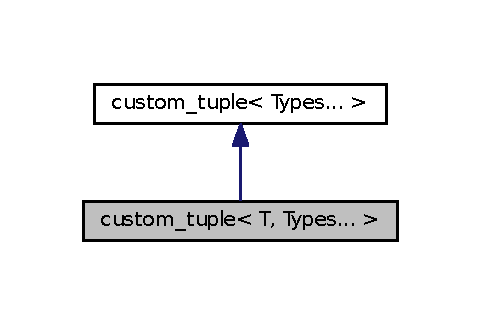
\includegraphics[width=231pt]{structcustom__tuple_3_01T_00_01Types_8_8_8_01_4__inherit__graph}
\end{center}
\end{figure}


Collaboration diagram for custom\+\_\+tuple$<$ T, Types... $>$\+:
\nopagebreak
\begin{figure}[H]
\begin{center}
\leavevmode
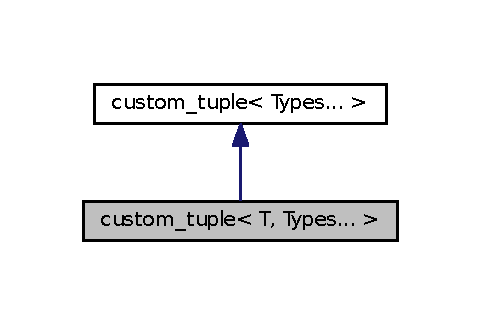
\includegraphics[width=231pt]{structcustom__tuple_3_01T_00_01Types_8_8_8_01_4__coll__graph}
\end{center}
\end{figure}
\subsection*{Public Member Functions}
\begin{DoxyCompactItemize}
\item 
\hyperlink{structcustom__tuple_3_01T_00_01Types_8_8_8_01_4_a89f0b4cc59a4efeb82f0160541708f9a}{custom\+\_\+tuple} (T t\+\_\+arg, Types...\+ts\+\_\+args)
\item 
{\footnotesize template$<$typename Arg1 , typename... Args$>$ }\\\hyperlink{structcustom__tuple}{custom\+\_\+tuple} \& \hyperlink{structcustom__tuple_3_01T_00_01Types_8_8_8_01_4_a40eac7f8ba44f72911adfad9239f91df}{operator=} (const \hyperlink{structcustom__tuple}{custom\+\_\+tuple}$<$ Arg1, Args... $>$ \&rhs)
\item 
{\footnotesize template$<$typename Arg1 , typename... Args$>$ }\\\hyperlink{structcustom__tuple}{custom\+\_\+tuple}$<$ T, Types... $>$ \& \hyperlink{structcustom__tuple_3_01T_00_01Types_8_8_8_01_4_a5bc95f94e20d4b02e3c80eef3e2f7036}{operator=} (const \hyperlink{structcustom__tuple}{custom\+\_\+tuple}$<$ Arg1, Args... $>$ \&rhs)
\end{DoxyCompactItemize}
\subsection*{Public Attributes}
\begin{DoxyCompactItemize}
\item 
T \hyperlink{structcustom__tuple_3_01T_00_01Types_8_8_8_01_4_adff61bc9ff136d4c8393278eef6b62b4}{tail}
\end{DoxyCompactItemize}


\subsection{Constructor \& Destructor Documentation}
\index{custom\+\_\+tuple$<$ T, Types... $>$@{custom\+\_\+tuple$<$ T, Types... $>$}!custom\+\_\+tuple@{custom\+\_\+tuple}}
\index{custom\+\_\+tuple@{custom\+\_\+tuple}!custom\+\_\+tuple$<$ T, Types... $>$@{custom\+\_\+tuple$<$ T, Types... $>$}}
\subsubsection[{\texorpdfstring{custom\+\_\+tuple(\+T t\+\_\+arg, Types...\+ts\+\_\+args)}{custom_tuple(T t_arg, Types...ts_args)}}]{\setlength{\rightskip}{0pt plus 5cm}template$<$typename T , typename... Types$>$ {\bf custom\+\_\+tuple}$<$ T, Types... $>$\+::{\bf custom\+\_\+tuple} (
\begin{DoxyParamCaption}
\item[{T}]{t\+\_\+arg, }
\item[{Types...}]{ts\+\_\+args}
\end{DoxyParamCaption}
)\hspace{0.3cm}{\ttfamily [inline]}}\hypertarget{structcustom__tuple_3_01T_00_01Types_8_8_8_01_4_a89f0b4cc59a4efeb82f0160541708f9a}{}\label{structcustom__tuple_3_01T_00_01Types_8_8_8_01_4_a89f0b4cc59a4efeb82f0160541708f9a}


\subsection{Member Function Documentation}
\index{custom\+\_\+tuple$<$ T, Types... $>$@{custom\+\_\+tuple$<$ T, Types... $>$}!operator=@{operator=}}
\index{operator=@{operator=}!custom\+\_\+tuple$<$ T, Types... $>$@{custom\+\_\+tuple$<$ T, Types... $>$}}
\subsubsection[{\texorpdfstring{operator=(const custom\+\_\+tuple$<$ Arg1, Args... $>$ \&rhs)}{operator=(const custom_tuple< Arg1, Args... > &rhs)}}]{\setlength{\rightskip}{0pt plus 5cm}template$<$typename T , typename... Types$>$ template$<$typename Arg1 , typename... Args$>$ {\bf custom\+\_\+tuple}\& {\bf custom\+\_\+tuple}$<$ T, Types... $>$\+::operator= (
\begin{DoxyParamCaption}
\item[{const {\bf custom\+\_\+tuple}$<$ Arg1, Args... $>$ \&}]{rhs}
\end{DoxyParamCaption}
)}\hypertarget{structcustom__tuple_3_01T_00_01Types_8_8_8_01_4_a40eac7f8ba44f72911adfad9239f91df}{}\label{structcustom__tuple_3_01T_00_01Types_8_8_8_01_4_a40eac7f8ba44f72911adfad9239f91df}
\index{custom\+\_\+tuple$<$ T, Types... $>$@{custom\+\_\+tuple$<$ T, Types... $>$}!operator=@{operator=}}
\index{operator=@{operator=}!custom\+\_\+tuple$<$ T, Types... $>$@{custom\+\_\+tuple$<$ T, Types... $>$}}
\subsubsection[{\texorpdfstring{operator=(const custom\+\_\+tuple$<$ Arg1, Args... $>$ \&rhs)}{operator=(const custom_tuple< Arg1, Args... > &rhs)}}]{\setlength{\rightskip}{0pt plus 5cm}template$<$typename T , typename... Types$>$ template$<$typename Arg1 , typename... Args$>$ {\bf custom\+\_\+tuple}$<$T, Types ... $>$\& {\bf custom\+\_\+tuple}$<$ T, Types... $>$\+::operator= (
\begin{DoxyParamCaption}
\item[{const {\bf custom\+\_\+tuple}$<$ Arg1, Args... $>$ \&}]{rhs}
\end{DoxyParamCaption}
)}\hypertarget{structcustom__tuple_3_01T_00_01Types_8_8_8_01_4_a5bc95f94e20d4b02e3c80eef3e2f7036}{}\label{structcustom__tuple_3_01T_00_01Types_8_8_8_01_4_a5bc95f94e20d4b02e3c80eef3e2f7036}


\subsection{Member Data Documentation}
\index{custom\+\_\+tuple$<$ T, Types... $>$@{custom\+\_\+tuple$<$ T, Types... $>$}!tail@{tail}}
\index{tail@{tail}!custom\+\_\+tuple$<$ T, Types... $>$@{custom\+\_\+tuple$<$ T, Types... $>$}}
\subsubsection[{\texorpdfstring{tail}{tail}}]{\setlength{\rightskip}{0pt plus 5cm}template$<$typename T , typename... Types$>$ T {\bf custom\+\_\+tuple}$<$ T, Types... $>$\+::tail}\hypertarget{structcustom__tuple_3_01T_00_01Types_8_8_8_01_4_adff61bc9ff136d4c8393278eef6b62b4}{}\label{structcustom__tuple_3_01T_00_01Types_8_8_8_01_4_adff61bc9ff136d4c8393278eef6b62b4}


The documentation for this struct was generated from the following file\+:\begin{DoxyCompactItemize}
\item 
02\+\_\+tuple/\hyperlink{cstm__tuple_8hpp}{cstm\+\_\+tuple.\+hpp}\end{DoxyCompactItemize}

\hypertarget{classCustomContainer}{}\section{Custom\+Container$<$ T, allocator\+\_\+type $>$ Class Template Reference}
\label{classCustomContainer}\index{Custom\+Container$<$ T, allocator\+\_\+type $>$@{Custom\+Container$<$ T, allocator\+\_\+type $>$}}


{\ttfamily \#include $<$custom\+\_\+container.\+hpp$>$}

\subsection*{Public Member Functions}
\begin{DoxyCompactItemize}
\item 
\hyperlink{classCustomContainer_a897f80c9a60a7f9258dabb8001010baa}{Custom\+Container} ()
\item 
\hyperlink{classCustomContainer_a7de15b5199e301225c6bc469aef4ef77}{$\sim$\+Custom\+Container} ()
\item 
void \hyperlink{classCustomContainer_a157d34d3688751810f744f7a3c57ea9b}{push\+\_\+back} (T item)
\item 
T \& \hyperlink{classCustomContainer_a033b74212eb7179ce7743ae58a7d2233}{current\+\_\+item} ()
\item 
void \hyperlink{classCustomContainer_a6cd396f303782097efc8eff705a720b8}{to\+\_\+begin} ()
\item 
bool \hyperlink{classCustomContainer_a5be4653f018c8c83e863221ce34c7ab1}{next} ()
\end{DoxyCompactItemize}


\subsection{Constructor \& Destructor Documentation}
\index{Custom\+Container@{Custom\+Container}!Custom\+Container@{Custom\+Container}}
\index{Custom\+Container@{Custom\+Container}!Custom\+Container@{Custom\+Container}}
\subsubsection[{\texorpdfstring{Custom\+Container()}{CustomContainer()}}]{\setlength{\rightskip}{0pt plus 5cm}template$<$typename T , typename allocator\+\_\+type $>$ {\bf Custom\+Container}$<$ T, allocator\+\_\+type $>$\+::{\bf Custom\+Container} (
\begin{DoxyParamCaption}
{}
\end{DoxyParamCaption}
)}\hypertarget{classCustomContainer_a897f80c9a60a7f9258dabb8001010baa}{}\label{classCustomContainer_a897f80c9a60a7f9258dabb8001010baa}
\index{Custom\+Container@{Custom\+Container}!````~Custom\+Container@{$\sim$\+Custom\+Container}}
\index{````~Custom\+Container@{$\sim$\+Custom\+Container}!Custom\+Container@{Custom\+Container}}
\subsubsection[{\texorpdfstring{$\sim$\+Custom\+Container()}{~CustomContainer()}}]{\setlength{\rightskip}{0pt plus 5cm}template$<$typename T , typename allocator\+\_\+type $>$ {\bf Custom\+Container}$<$ T, allocator\+\_\+type $>$\+::$\sim${\bf Custom\+Container} (
\begin{DoxyParamCaption}
{}
\end{DoxyParamCaption}
)}\hypertarget{classCustomContainer_a7de15b5199e301225c6bc469aef4ef77}{}\label{classCustomContainer_a7de15b5199e301225c6bc469aef4ef77}


\subsection{Member Function Documentation}
\index{Custom\+Container@{Custom\+Container}!current\+\_\+item@{current\+\_\+item}}
\index{current\+\_\+item@{current\+\_\+item}!Custom\+Container@{Custom\+Container}}
\subsubsection[{\texorpdfstring{current\+\_\+item()}{current_item()}}]{\setlength{\rightskip}{0pt plus 5cm}template$<$typename T , typename allocator\+\_\+type $>$ T \& {\bf Custom\+Container}$<$ T, allocator\+\_\+type $>$\+::current\+\_\+item (
\begin{DoxyParamCaption}
{}
\end{DoxyParamCaption}
)}\hypertarget{classCustomContainer_a033b74212eb7179ce7743ae58a7d2233}{}\label{classCustomContainer_a033b74212eb7179ce7743ae58a7d2233}
\index{Custom\+Container@{Custom\+Container}!next@{next}}
\index{next@{next}!Custom\+Container@{Custom\+Container}}
\subsubsection[{\texorpdfstring{next()}{next()}}]{\setlength{\rightskip}{0pt plus 5cm}template$<$typename T , typename allocator\+\_\+type $>$ bool {\bf Custom\+Container}$<$ T, allocator\+\_\+type $>$\+::next (
\begin{DoxyParamCaption}
{}
\end{DoxyParamCaption}
)}\hypertarget{classCustomContainer_a5be4653f018c8c83e863221ce34c7ab1}{}\label{classCustomContainer_a5be4653f018c8c83e863221ce34c7ab1}
\index{Custom\+Container@{Custom\+Container}!push\+\_\+back@{push\+\_\+back}}
\index{push\+\_\+back@{push\+\_\+back}!Custom\+Container@{Custom\+Container}}
\subsubsection[{\texorpdfstring{push\+\_\+back(\+T item)}{push_back(T item)}}]{\setlength{\rightskip}{0pt plus 5cm}template$<$typename T , typename allocator\+\_\+type $>$ void {\bf Custom\+Container}$<$ T, allocator\+\_\+type $>$\+::push\+\_\+back (
\begin{DoxyParamCaption}
\item[{T}]{item}
\end{DoxyParamCaption}
)}\hypertarget{classCustomContainer_a157d34d3688751810f744f7a3c57ea9b}{}\label{classCustomContainer_a157d34d3688751810f744f7a3c57ea9b}
\index{Custom\+Container@{Custom\+Container}!to\+\_\+begin@{to\+\_\+begin}}
\index{to\+\_\+begin@{to\+\_\+begin}!Custom\+Container@{Custom\+Container}}
\subsubsection[{\texorpdfstring{to\+\_\+begin()}{to_begin()}}]{\setlength{\rightskip}{0pt plus 5cm}template$<$typename T , typename allocator\+\_\+type $>$ void {\bf Custom\+Container}$<$ T, allocator\+\_\+type $>$\+::to\+\_\+begin (
\begin{DoxyParamCaption}
{}
\end{DoxyParamCaption}
)}\hypertarget{classCustomContainer_a6cd396f303782097efc8eff705a720b8}{}\label{classCustomContainer_a6cd396f303782097efc8eff705a720b8}


The documentation for this class was generated from the following file\+:\begin{DoxyCompactItemize}
\item 
03\+\_\+allocator/\hyperlink{custom__container_8hpp}{custom\+\_\+container.\+hpp}\end{DoxyCompactItemize}

\hypertarget{classCustomContainer_3_01T_00_01reserve__allocator_3_01T_00_01n_01_4_01_4}{}\section{Custom\+Container$<$ T, reserve\+\_\+allocator$<$ T, n $>$ $>$ Class Template Reference}
\label{classCustomContainer_3_01T_00_01reserve__allocator_3_01T_00_01n_01_4_01_4}\index{Custom\+Container$<$ T, reserve\+\_\+allocator$<$ T, n $>$ $>$@{Custom\+Container$<$ T, reserve\+\_\+allocator$<$ T, n $>$ $>$}}


{\ttfamily \#include $<$reserved\+\_\+container.\+hpp$>$}

\subsection*{Public Member Functions}
\begin{DoxyCompactItemize}
\item 
\hyperlink{classCustomContainer_3_01T_00_01reserve__allocator_3_01T_00_01n_01_4_01_4_a330b8e1e23a306434468ad69baeb2ee7}{Custom\+Container} ()
\item 
\hyperlink{classCustomContainer_3_01T_00_01reserve__allocator_3_01T_00_01n_01_4_01_4_a11dae533731736ae4c2309550b793a11}{$\sim$\+Custom\+Container} ()
\item 
void \hyperlink{classCustomContainer_3_01T_00_01reserve__allocator_3_01T_00_01n_01_4_01_4_a7b41f31f5e430ff461b3e906be789058}{push\+\_\+back} (T item)
\item 
T \& \hyperlink{classCustomContainer_3_01T_00_01reserve__allocator_3_01T_00_01n_01_4_01_4_ab6557ab6a4eb23ee58f6aa42e49e87cc}{current\+\_\+item} ()
\item 
void \hyperlink{classCustomContainer_3_01T_00_01reserve__allocator_3_01T_00_01n_01_4_01_4_aa43a96f008af53f254a014629f0627b7}{to\+\_\+begin} ()
\item 
bool \hyperlink{classCustomContainer_3_01T_00_01reserve__allocator_3_01T_00_01n_01_4_01_4_a1714165f87a1ae507e39b97e8a0bda90}{next} ()
\end{DoxyCompactItemize}


\subsection{Constructor \& Destructor Documentation}
\index{Custom\+Container$<$ T, reserve\+\_\+allocator$<$ T, n $>$ $>$@{Custom\+Container$<$ T, reserve\+\_\+allocator$<$ T, n $>$ $>$}!Custom\+Container@{Custom\+Container}}
\index{Custom\+Container@{Custom\+Container}!Custom\+Container$<$ T, reserve\+\_\+allocator$<$ T, n $>$ $>$@{Custom\+Container$<$ T, reserve\+\_\+allocator$<$ T, n $>$ $>$}}
\subsubsection[{\texorpdfstring{Custom\+Container()}{CustomContainer()}}]{\setlength{\rightskip}{0pt plus 5cm}template$<$typename T , size\+\_\+t n$>$ {\bf Custom\+Container}$<$ T, {\bf reserve\+\_\+allocator}$<$ T, n $>$ $>$\+::{\bf Custom\+Container} (
\begin{DoxyParamCaption}
{}
\end{DoxyParamCaption}
)}\hypertarget{classCustomContainer_3_01T_00_01reserve__allocator_3_01T_00_01n_01_4_01_4_a330b8e1e23a306434468ad69baeb2ee7}{}\label{classCustomContainer_3_01T_00_01reserve__allocator_3_01T_00_01n_01_4_01_4_a330b8e1e23a306434468ad69baeb2ee7}
\index{Custom\+Container$<$ T, reserve\+\_\+allocator$<$ T, n $>$ $>$@{Custom\+Container$<$ T, reserve\+\_\+allocator$<$ T, n $>$ $>$}!````~Custom\+Container@{$\sim$\+Custom\+Container}}
\index{````~Custom\+Container@{$\sim$\+Custom\+Container}!Custom\+Container$<$ T, reserve\+\_\+allocator$<$ T, n $>$ $>$@{Custom\+Container$<$ T, reserve\+\_\+allocator$<$ T, n $>$ $>$}}
\subsubsection[{\texorpdfstring{$\sim$\+Custom\+Container()}{~CustomContainer()}}]{\setlength{\rightskip}{0pt plus 5cm}template$<$typename T , size\+\_\+t n$>$ {\bf Custom\+Container}$<$ T, {\bf reserve\+\_\+allocator}$<$ T, n $>$ $>$\+::$\sim${\bf Custom\+Container} (
\begin{DoxyParamCaption}
{}
\end{DoxyParamCaption}
)}\hypertarget{classCustomContainer_3_01T_00_01reserve__allocator_3_01T_00_01n_01_4_01_4_a11dae533731736ae4c2309550b793a11}{}\label{classCustomContainer_3_01T_00_01reserve__allocator_3_01T_00_01n_01_4_01_4_a11dae533731736ae4c2309550b793a11}


\subsection{Member Function Documentation}
\index{Custom\+Container$<$ T, reserve\+\_\+allocator$<$ T, n $>$ $>$@{Custom\+Container$<$ T, reserve\+\_\+allocator$<$ T, n $>$ $>$}!current\+\_\+item@{current\+\_\+item}}
\index{current\+\_\+item@{current\+\_\+item}!Custom\+Container$<$ T, reserve\+\_\+allocator$<$ T, n $>$ $>$@{Custom\+Container$<$ T, reserve\+\_\+allocator$<$ T, n $>$ $>$}}
\subsubsection[{\texorpdfstring{current\+\_\+item()}{current_item()}}]{\setlength{\rightskip}{0pt plus 5cm}template$<$typename T , size\+\_\+t n$>$ T \& {\bf Custom\+Container}$<$ T, {\bf reserve\+\_\+allocator}$<$ T, n $>$ $>$\+::current\+\_\+item (
\begin{DoxyParamCaption}
{}
\end{DoxyParamCaption}
)}\hypertarget{classCustomContainer_3_01T_00_01reserve__allocator_3_01T_00_01n_01_4_01_4_ab6557ab6a4eb23ee58f6aa42e49e87cc}{}\label{classCustomContainer_3_01T_00_01reserve__allocator_3_01T_00_01n_01_4_01_4_ab6557ab6a4eb23ee58f6aa42e49e87cc}
\index{Custom\+Container$<$ T, reserve\+\_\+allocator$<$ T, n $>$ $>$@{Custom\+Container$<$ T, reserve\+\_\+allocator$<$ T, n $>$ $>$}!next@{next}}
\index{next@{next}!Custom\+Container$<$ T, reserve\+\_\+allocator$<$ T, n $>$ $>$@{Custom\+Container$<$ T, reserve\+\_\+allocator$<$ T, n $>$ $>$}}
\subsubsection[{\texorpdfstring{next()}{next()}}]{\setlength{\rightskip}{0pt plus 5cm}template$<$typename T , size\+\_\+t n$>$ bool {\bf Custom\+Container}$<$ T, {\bf reserve\+\_\+allocator}$<$ T, n $>$ $>$\+::next (
\begin{DoxyParamCaption}
{}
\end{DoxyParamCaption}
)}\hypertarget{classCustomContainer_3_01T_00_01reserve__allocator_3_01T_00_01n_01_4_01_4_a1714165f87a1ae507e39b97e8a0bda90}{}\label{classCustomContainer_3_01T_00_01reserve__allocator_3_01T_00_01n_01_4_01_4_a1714165f87a1ae507e39b97e8a0bda90}
\index{Custom\+Container$<$ T, reserve\+\_\+allocator$<$ T, n $>$ $>$@{Custom\+Container$<$ T, reserve\+\_\+allocator$<$ T, n $>$ $>$}!push\+\_\+back@{push\+\_\+back}}
\index{push\+\_\+back@{push\+\_\+back}!Custom\+Container$<$ T, reserve\+\_\+allocator$<$ T, n $>$ $>$@{Custom\+Container$<$ T, reserve\+\_\+allocator$<$ T, n $>$ $>$}}
\subsubsection[{\texorpdfstring{push\+\_\+back(\+T item)}{push_back(T item)}}]{\setlength{\rightskip}{0pt plus 5cm}template$<$typename T , size\+\_\+t n$>$ void {\bf Custom\+Container}$<$ T, {\bf reserve\+\_\+allocator}$<$ T, n $>$ $>$\+::push\+\_\+back (
\begin{DoxyParamCaption}
\item[{T}]{item}
\end{DoxyParamCaption}
)}\hypertarget{classCustomContainer_3_01T_00_01reserve__allocator_3_01T_00_01n_01_4_01_4_a7b41f31f5e430ff461b3e906be789058}{}\label{classCustomContainer_3_01T_00_01reserve__allocator_3_01T_00_01n_01_4_01_4_a7b41f31f5e430ff461b3e906be789058}
\index{Custom\+Container$<$ T, reserve\+\_\+allocator$<$ T, n $>$ $>$@{Custom\+Container$<$ T, reserve\+\_\+allocator$<$ T, n $>$ $>$}!to\+\_\+begin@{to\+\_\+begin}}
\index{to\+\_\+begin@{to\+\_\+begin}!Custom\+Container$<$ T, reserve\+\_\+allocator$<$ T, n $>$ $>$@{Custom\+Container$<$ T, reserve\+\_\+allocator$<$ T, n $>$ $>$}}
\subsubsection[{\texorpdfstring{to\+\_\+begin()}{to_begin()}}]{\setlength{\rightskip}{0pt plus 5cm}template$<$typename T , size\+\_\+t n$>$ void {\bf Custom\+Container}$<$ T, {\bf reserve\+\_\+allocator}$<$ T, n $>$ $>$\+::to\+\_\+begin (
\begin{DoxyParamCaption}
{}
\end{DoxyParamCaption}
)}\hypertarget{classCustomContainer_3_01T_00_01reserve__allocator_3_01T_00_01n_01_4_01_4_aa43a96f008af53f254a014629f0627b7}{}\label{classCustomContainer_3_01T_00_01reserve__allocator_3_01T_00_01n_01_4_01_4_aa43a96f008af53f254a014629f0627b7}


The documentation for this class was generated from the following file\+:\begin{DoxyCompactItemize}
\item 
03\+\_\+allocator/\hyperlink{reserved__container_8hpp}{reserved\+\_\+container.\+hpp}\end{DoxyCompactItemize}

\hypertarget{classCustomPair}{}\section{Custom\+Pair$<$ T1, U2 $>$ Class Template Reference}
\label{classCustomPair}\index{Custom\+Pair$<$ T1, U2 $>$@{Custom\+Pair$<$ T1, U2 $>$}}


{\ttfamily \#include $<$cstm\+\_\+pair.\+hpp$>$}

\subsection*{Public Member Functions}
\begin{DoxyCompactItemize}
\item 
\hyperlink{classCustomPair_a08267c93486d41377a8403e1e7109c4f}{Custom\+Pair} ()
\item 
\hyperlink{classCustomPair_abdaebfaee7292d2c83fb68373a5b19ca}{Custom\+Pair} (const T1 \&f, const U2 \&s)
\item 
\hyperlink{classCustomPair_ac81e98af29d37f8df7d8199f8185d4be}{Custom\+Pair} (T1 \&\&f, U2 \&\&s)
\item 
\hyperlink{classCustomPair_ad9b27b057afcf0bba10fd4ee27f6f336}{Custom\+Pair} (const \hyperlink{classCustomPair}{Custom\+Pair} \&rhs)
\item 
\hyperlink{classCustomPair_aeeabcac87aa65e6efc9cb3e2acd4cd2a}{Custom\+Pair} (\hyperlink{classCustomPair}{Custom\+Pair} \&\&rhs)
\item 
\hyperlink{classCustomPair}{Custom\+Pair} \& \hyperlink{classCustomPair_a0382ce4957c495f9d113feec0dd0fd0d}{operator=} (const \hyperlink{classCustomPair}{Custom\+Pair} \&)
\item 
\hyperlink{classCustomPair}{Custom\+Pair} \& \hyperlink{classCustomPair_a5eb9461e32ce141d4ac27312c36c6e4a}{operator=} (\hyperlink{classCustomPair}{Custom\+Pair} \&\&)
\item 
\hyperlink{classCustomPair_ac020a919f7416ce505190c396dc13d85}{$\sim$\+Custom\+Pair} ()
\item 
void \hyperlink{classCustomPair_af924734860d947883590406517cb56a8}{operator$>$$>$} (std\+::ostream \&os) const 
\item 
\hyperlink{classCustomPair}{Custom\+Pair} \hyperlink{classCustomPair_a7734ebd7a782940990888a46fc8e0b3e}{make\+\_\+custom\+\_\+pair} (T1 f, U2 s)
\end{DoxyCompactItemize}
\subsection*{Friends}
\begin{DoxyCompactItemize}
\item 
class \hyperlink{classCustomPair_a2736cfbb3ae5473b8409edf1a53709dd}{Custom\+Pair$<$ T1 \&, U2 \& $>$}
\item 
{\footnotesize template$<$size\+\_\+t n, typename arg1 , typename arg2 $>$ }\\std\+::enable\+\_\+if$<$ n==0, arg1 $>$\+::type \& \hyperlink{classCustomPair_a236d0006b206a258acc1424396b819de}{get} (\hyperlink{classCustomPair}{Custom\+Pair}$<$ arg1, arg2 $>$ \&)
\item 
{\footnotesize template$<$size\+\_\+t n, typename arg1 , typename arg2 $>$ }\\std\+::enable\+\_\+if$<$ n==1, arg2 $>$\+::type \& \hyperlink{classCustomPair_a5be88dc84aab345e8bf2058857498efc}{get} (\hyperlink{classCustomPair}{Custom\+Pair}$<$ arg1, arg2 $>$ \&)
\end{DoxyCompactItemize}


\subsection{Constructor \& Destructor Documentation}
\index{Custom\+Pair@{Custom\+Pair}!Custom\+Pair@{Custom\+Pair}}
\index{Custom\+Pair@{Custom\+Pair}!Custom\+Pair@{Custom\+Pair}}
\subsubsection[{\texorpdfstring{Custom\+Pair()}{CustomPair()}}]{\setlength{\rightskip}{0pt plus 5cm}template$<$typename T1 , typename U2 $>$ {\bf Custom\+Pair}$<$ T1, U2 $>$\+::{\bf Custom\+Pair} (
\begin{DoxyParamCaption}
{}
\end{DoxyParamCaption}
)}\hypertarget{classCustomPair_a08267c93486d41377a8403e1e7109c4f}{}\label{classCustomPair_a08267c93486d41377a8403e1e7109c4f}
\index{Custom\+Pair@{Custom\+Pair}!Custom\+Pair@{Custom\+Pair}}
\index{Custom\+Pair@{Custom\+Pair}!Custom\+Pair@{Custom\+Pair}}
\subsubsection[{\texorpdfstring{Custom\+Pair(const T1 \&f, const U2 \&s)}{CustomPair(const T1 &f, const U2 &s)}}]{\setlength{\rightskip}{0pt plus 5cm}template$<$typename T1 , typename U2 $>$ {\bf Custom\+Pair}$<$ T1, U2 $>$\+::{\bf Custom\+Pair} (
\begin{DoxyParamCaption}
\item[{const T1 \&}]{f, }
\item[{const U2 \&}]{s}
\end{DoxyParamCaption}
)}\hypertarget{classCustomPair_abdaebfaee7292d2c83fb68373a5b19ca}{}\label{classCustomPair_abdaebfaee7292d2c83fb68373a5b19ca}
\index{Custom\+Pair@{Custom\+Pair}!Custom\+Pair@{Custom\+Pair}}
\index{Custom\+Pair@{Custom\+Pair}!Custom\+Pair@{Custom\+Pair}}
\subsubsection[{\texorpdfstring{Custom\+Pair(\+T1 \&\&f, U2 \&\&s)}{CustomPair(T1 &&f, U2 &&s)}}]{\setlength{\rightskip}{0pt plus 5cm}template$<$typename T1 , typename U2 $>$ {\bf Custom\+Pair}$<$ T1, U2 $>$\+::{\bf Custom\+Pair} (
\begin{DoxyParamCaption}
\item[{T1 \&\&}]{f, }
\item[{U2 \&\&}]{s}
\end{DoxyParamCaption}
)}\hypertarget{classCustomPair_ac81e98af29d37f8df7d8199f8185d4be}{}\label{classCustomPair_ac81e98af29d37f8df7d8199f8185d4be}
\index{Custom\+Pair@{Custom\+Pair}!Custom\+Pair@{Custom\+Pair}}
\index{Custom\+Pair@{Custom\+Pair}!Custom\+Pair@{Custom\+Pair}}
\subsubsection[{\texorpdfstring{Custom\+Pair(const Custom\+Pair \&rhs)}{CustomPair(const CustomPair &rhs)}}]{\setlength{\rightskip}{0pt plus 5cm}template$<$typename T1 , typename U2 $>$ {\bf Custom\+Pair}$<$ T1, U2 $>$\+::{\bf Custom\+Pair} (
\begin{DoxyParamCaption}
\item[{const {\bf Custom\+Pair}$<$ T1, U2 $>$ \&}]{rhs}
\end{DoxyParamCaption}
)}\hypertarget{classCustomPair_ad9b27b057afcf0bba10fd4ee27f6f336}{}\label{classCustomPair_ad9b27b057afcf0bba10fd4ee27f6f336}
\index{Custom\+Pair@{Custom\+Pair}!Custom\+Pair@{Custom\+Pair}}
\index{Custom\+Pair@{Custom\+Pair}!Custom\+Pair@{Custom\+Pair}}
\subsubsection[{\texorpdfstring{Custom\+Pair(\+Custom\+Pair \&\&rhs)}{CustomPair(CustomPair &&rhs)}}]{\setlength{\rightskip}{0pt plus 5cm}template$<$typename T1 , typename U2 $>$ {\bf Custom\+Pair}$<$ T1, U2 $>$\+::{\bf Custom\+Pair} (
\begin{DoxyParamCaption}
\item[{{\bf Custom\+Pair}$<$ T1, U2 $>$ \&\&}]{rhs}
\end{DoxyParamCaption}
)}\hypertarget{classCustomPair_aeeabcac87aa65e6efc9cb3e2acd4cd2a}{}\label{classCustomPair_aeeabcac87aa65e6efc9cb3e2acd4cd2a}
\index{Custom\+Pair@{Custom\+Pair}!````~Custom\+Pair@{$\sim$\+Custom\+Pair}}
\index{````~Custom\+Pair@{$\sim$\+Custom\+Pair}!Custom\+Pair@{Custom\+Pair}}
\subsubsection[{\texorpdfstring{$\sim$\+Custom\+Pair()}{~CustomPair()}}]{\setlength{\rightskip}{0pt plus 5cm}template$<$typename T1 , typename U2 $>$ {\bf Custom\+Pair}$<$ T1, U2 $>$\+::$\sim${\bf Custom\+Pair} (
\begin{DoxyParamCaption}
{}
\end{DoxyParamCaption}
)}\hypertarget{classCustomPair_ac020a919f7416ce505190c396dc13d85}{}\label{classCustomPair_ac020a919f7416ce505190c396dc13d85}


\subsection{Member Function Documentation}
\index{Custom\+Pair@{Custom\+Pair}!make\+\_\+custom\+\_\+pair@{make\+\_\+custom\+\_\+pair}}
\index{make\+\_\+custom\+\_\+pair@{make\+\_\+custom\+\_\+pair}!Custom\+Pair@{Custom\+Pair}}
\subsubsection[{\texorpdfstring{make\+\_\+custom\+\_\+pair(\+T1 f, U2 s)}{make_custom_pair(T1 f, U2 s)}}]{\setlength{\rightskip}{0pt plus 5cm}template$<$typename T1, typename U2$>$ {\bf Custom\+Pair} {\bf Custom\+Pair}$<$ T1, U2 $>$\+::make\+\_\+custom\+\_\+pair (
\begin{DoxyParamCaption}
\item[{T1}]{f, }
\item[{U2}]{s}
\end{DoxyParamCaption}
)}\hypertarget{classCustomPair_a7734ebd7a782940990888a46fc8e0b3e}{}\label{classCustomPair_a7734ebd7a782940990888a46fc8e0b3e}
\index{Custom\+Pair@{Custom\+Pair}!operator=@{operator=}}
\index{operator=@{operator=}!Custom\+Pair@{Custom\+Pair}}
\subsubsection[{\texorpdfstring{operator=(const Custom\+Pair \&)}{operator=(const CustomPair &)}}]{\setlength{\rightskip}{0pt plus 5cm}template$<$typename T1 , typename U2 $>$ {\bf Custom\+Pair}$<$ T1, U2 $>$ \& {\bf Custom\+Pair}$<$ T1, U2 $>$\+::operator= (
\begin{DoxyParamCaption}
\item[{const {\bf Custom\+Pair}$<$ T1, U2 $>$ \&}]{rhs}
\end{DoxyParamCaption}
)}\hypertarget{classCustomPair_a0382ce4957c495f9d113feec0dd0fd0d}{}\label{classCustomPair_a0382ce4957c495f9d113feec0dd0fd0d}
\index{Custom\+Pair@{Custom\+Pair}!operator=@{operator=}}
\index{operator=@{operator=}!Custom\+Pair@{Custom\+Pair}}
\subsubsection[{\texorpdfstring{operator=(\+Custom\+Pair \&\&)}{operator=(CustomPair &&)}}]{\setlength{\rightskip}{0pt plus 5cm}template$<$typename T1 , typename U2 $>$ {\bf Custom\+Pair}$<$ T1, U2 $>$ \& {\bf Custom\+Pair}$<$ T1, U2 $>$\+::operator= (
\begin{DoxyParamCaption}
\item[{{\bf Custom\+Pair}$<$ T1, U2 $>$ \&\&}]{rhs}
\end{DoxyParamCaption}
)}\hypertarget{classCustomPair_a5eb9461e32ce141d4ac27312c36c6e4a}{}\label{classCustomPair_a5eb9461e32ce141d4ac27312c36c6e4a}
\index{Custom\+Pair@{Custom\+Pair}!operator$>$$>$@{operator$>$$>$}}
\index{operator$>$$>$@{operator$>$$>$}!Custom\+Pair@{Custom\+Pair}}
\subsubsection[{\texorpdfstring{operator$>$$>$(std\+::ostream \&os) const }{operator>>(std::ostream &os) const }}]{\setlength{\rightskip}{0pt plus 5cm}template$<$typename T1 , typename U2 $>$ void {\bf Custom\+Pair}$<$ T1, U2 $>$\+::operator$>$$>$ (
\begin{DoxyParamCaption}
\item[{std\+::ostream \&}]{os}
\end{DoxyParamCaption}
) const}\hypertarget{classCustomPair_af924734860d947883590406517cb56a8}{}\label{classCustomPair_af924734860d947883590406517cb56a8}


\subsection{Friends And Related Function Documentation}
\index{Custom\+Pair@{Custom\+Pair}!Custom\+Pair$<$ T1 \&, U2 \& $>$@{Custom\+Pair$<$ T1 \&, U2 \& $>$}}
\index{Custom\+Pair$<$ T1 \&, U2 \& $>$@{Custom\+Pair$<$ T1 \&, U2 \& $>$}!Custom\+Pair@{Custom\+Pair}}
\subsubsection[{\texorpdfstring{Custom\+Pair$<$ T1 \&, U2 \& $>$}{CustomPair< T1 &, U2 & >}}]{\setlength{\rightskip}{0pt plus 5cm}template$<$typename T1, typename U2$>$ friend class {\bf Custom\+Pair}$<$ T1 \&, U2 \& $>$\hspace{0.3cm}{\ttfamily [friend]}}\hypertarget{classCustomPair_a2736cfbb3ae5473b8409edf1a53709dd}{}\label{classCustomPair_a2736cfbb3ae5473b8409edf1a53709dd}
\index{Custom\+Pair@{Custom\+Pair}!get@{get}}
\index{get@{get}!Custom\+Pair@{Custom\+Pair}}
\subsubsection[{\texorpdfstring{get}{get}}]{\setlength{\rightskip}{0pt plus 5cm}template$<$typename T1, typename U2$>$ template$<$size\+\_\+t n, typename arg1 , typename arg2 $>$ std\+::enable\+\_\+if$<$n == 0, arg1$>$\+::type\& get (
\begin{DoxyParamCaption}
\item[{{\bf Custom\+Pair}$<$ arg1, arg2 $>$ \&}]{}
\end{DoxyParamCaption}
)\hspace{0.3cm}{\ttfamily [friend]}}\hypertarget{classCustomPair_a236d0006b206a258acc1424396b819de}{}\label{classCustomPair_a236d0006b206a258acc1424396b819de}
\index{Custom\+Pair@{Custom\+Pair}!get@{get}}
\index{get@{get}!Custom\+Pair@{Custom\+Pair}}
\subsubsection[{\texorpdfstring{get}{get}}]{\setlength{\rightskip}{0pt plus 5cm}template$<$typename T1, typename U2$>$ template$<$size\+\_\+t n, typename arg1 , typename arg2 $>$ std\+::enable\+\_\+if$<$n == 1, arg2$>$\+::type\& get (
\begin{DoxyParamCaption}
\item[{{\bf Custom\+Pair}$<$ arg1, arg2 $>$ \&}]{}
\end{DoxyParamCaption}
)\hspace{0.3cm}{\ttfamily [friend]}}\hypertarget{classCustomPair_a5be88dc84aab345e8bf2058857498efc}{}\label{classCustomPair_a5be88dc84aab345e8bf2058857498efc}


The documentation for this class was generated from the following file\+:\begin{DoxyCompactItemize}
\item 
02\+\_\+tuple/\hyperlink{cstm__pair_8hpp}{cstm\+\_\+pair.\+hpp}\end{DoxyCompactItemize}

\hypertarget{classCustomPair2}{}\section{Custom\+Pair2$<$ T1, U2 $>$ Class Template Reference}
\label{classCustomPair2}\index{Custom\+Pair2$<$ T1, U2 $>$@{Custom\+Pair2$<$ T1, U2 $>$}}


{\ttfamily \#include $<$cstm\+\_\+pair\+\_\+2.\+hpp$>$}

\subsection*{Public Member Functions}
\begin{DoxyCompactItemize}
\item 
\hyperlink{classCustomPair2_a736df3b473094a2ad25aea58362db38b}{Custom\+Pair2} ()
\item 
\hyperlink{classCustomPair2_a917f5f777f4fea2a9dc70e79394624a7}{Custom\+Pair2} (const T1 \&f, const U2 \&s)
\item 
\hyperlink{classCustomPair2_a726068d9ffb66e66aff43501b4272179}{Custom\+Pair2} (const \hyperlink{classCustomPair2}{Custom\+Pair2} \&rhs)
\item 
\hyperlink{classCustomPair2}{Custom\+Pair2} \& \hyperlink{classCustomPair2_af3b1fa5b7441355be8bfa96d089ab37b}{operator=} (const \hyperlink{classCustomPair2}{Custom\+Pair2} \&)
\item 
\hyperlink{classCustomPair2}{Custom\+Pair2} \& \hyperlink{classCustomPair2_a5ae55c15931cd1a095a8fad4bcde724c}{operator=} (\hyperlink{classCustomPair2}{Custom\+Pair2} \&\&)
\item 
{\footnotesize template$<$typename Arg1 , typename Arg2 $>$ }\\\hyperlink{classCustomPair2}{Custom\+Pair2} \& \hyperlink{classCustomPair2_af68d83bfd286f5e0d7114d62a2dcc43e}{operator=} (const \hyperlink{classCustomPair2}{Custom\+Pair2}$<$ Arg1, Arg2 $>$ \&rhs)
\item 
\hyperlink{classCustomPair2_a2f6ff855e4378a0ae55fa0f74bb21219}{$\sim$\+Custom\+Pair2} ()
\item 
void \hyperlink{classCustomPair2_a6636532dcffffc8d3d8a4568fef36de4}{operator$>$$>$} (std\+::ostream \&os) const 
\item 
\hyperlink{classCustomPair2}{Custom\+Pair2} \hyperlink{classCustomPair2_a976ab888244d80a6020b34f3c3ff124f}{make\+\_\+custom\+\_\+pair} (T1 f, U2 s)
\item 
{\footnotesize template$<$typename Arg1 , typename Arg2 $>$ }\\\hyperlink{classCustomPair2}{Custom\+Pair2}$<$ T1, U2 $>$ \& \hyperlink{classCustomPair2_afeb8043ca6439aa32647cb3d5e6e7cd0}{operator=} (const \hyperlink{classCustomPair2}{Custom\+Pair2}$<$ Arg1, Arg2 $>$ \&rhs)
\end{DoxyCompactItemize}
\subsection*{Friends}
\begin{DoxyCompactItemize}
\item 
{\footnotesize template$<$typename Arg1 , typename Arg2 $>$ }\\class \hyperlink{classCustomPair2_a9641839d095886a143488ccb8d90dcd8}{Custom\+Pair2}
\item 
{\footnotesize template$<$size\+\_\+t n, typename arg1 , typename arg2 $>$ }\\std\+::enable\+\_\+if$<$ n==0, arg1 $>$\+::type \& \hyperlink{classCustomPair2_a9a2c35ed6198829fc94f69212024914a}{get} (\hyperlink{classCustomPair2}{Custom\+Pair2}$<$ arg1, arg2 $>$ \&)
\item 
{\footnotesize template$<$size\+\_\+t n, typename arg1 , typename arg2 $>$ }\\std\+::enable\+\_\+if$<$ n==1, arg2 $>$\+::type \& \hyperlink{classCustomPair2_a0c1d25e29757d03273b22572f3baaf96}{get} (\hyperlink{classCustomPair2}{Custom\+Pair2}$<$ arg1, arg2 $>$ \&)
\end{DoxyCompactItemize}


\subsection{Constructor \& Destructor Documentation}
\index{Custom\+Pair2@{Custom\+Pair2}!Custom\+Pair2@{Custom\+Pair2}}
\index{Custom\+Pair2@{Custom\+Pair2}!Custom\+Pair2@{Custom\+Pair2}}
\subsubsection[{\texorpdfstring{Custom\+Pair2()}{CustomPair2()}}]{\setlength{\rightskip}{0pt plus 5cm}template$<$typename T1 , typename U2 $>$ {\bf Custom\+Pair2}$<$ T1, U2 $>$\+::{\bf Custom\+Pair2} (
\begin{DoxyParamCaption}
{}
\end{DoxyParamCaption}
)}\hypertarget{classCustomPair2_a736df3b473094a2ad25aea58362db38b}{}\label{classCustomPair2_a736df3b473094a2ad25aea58362db38b}
\index{Custom\+Pair2@{Custom\+Pair2}!Custom\+Pair2@{Custom\+Pair2}}
\index{Custom\+Pair2@{Custom\+Pair2}!Custom\+Pair2@{Custom\+Pair2}}
\subsubsection[{\texorpdfstring{Custom\+Pair2(const T1 \&f, const U2 \&s)}{CustomPair2(const T1 &f, const U2 &s)}}]{\setlength{\rightskip}{0pt plus 5cm}template$<$typename T1 , typename U2 $>$ {\bf Custom\+Pair2}$<$ T1, U2 $>$\+::{\bf Custom\+Pair2} (
\begin{DoxyParamCaption}
\item[{const T1 \&}]{f, }
\item[{const U2 \&}]{s}
\end{DoxyParamCaption}
)}\hypertarget{classCustomPair2_a917f5f777f4fea2a9dc70e79394624a7}{}\label{classCustomPair2_a917f5f777f4fea2a9dc70e79394624a7}
\index{Custom\+Pair2@{Custom\+Pair2}!Custom\+Pair2@{Custom\+Pair2}}
\index{Custom\+Pair2@{Custom\+Pair2}!Custom\+Pair2@{Custom\+Pair2}}
\subsubsection[{\texorpdfstring{Custom\+Pair2(const Custom\+Pair2 \&rhs)}{CustomPair2(const CustomPair2 &rhs)}}]{\setlength{\rightskip}{0pt plus 5cm}template$<$typename T1 , typename U2 $>$ {\bf Custom\+Pair2}$<$ T1, U2 $>$\+::{\bf Custom\+Pair2} (
\begin{DoxyParamCaption}
\item[{const {\bf Custom\+Pair2}$<$ T1, U2 $>$ \&}]{rhs}
\end{DoxyParamCaption}
)}\hypertarget{classCustomPair2_a726068d9ffb66e66aff43501b4272179}{}\label{classCustomPair2_a726068d9ffb66e66aff43501b4272179}
\index{Custom\+Pair2@{Custom\+Pair2}!````~Custom\+Pair2@{$\sim$\+Custom\+Pair2}}
\index{````~Custom\+Pair2@{$\sim$\+Custom\+Pair2}!Custom\+Pair2@{Custom\+Pair2}}
\subsubsection[{\texorpdfstring{$\sim$\+Custom\+Pair2()}{~CustomPair2()}}]{\setlength{\rightskip}{0pt plus 5cm}template$<$typename T1 , typename U2 $>$ {\bf Custom\+Pair2}$<$ T1, U2 $>$\+::$\sim${\bf Custom\+Pair2} (
\begin{DoxyParamCaption}
{}
\end{DoxyParamCaption}
)}\hypertarget{classCustomPair2_a2f6ff855e4378a0ae55fa0f74bb21219}{}\label{classCustomPair2_a2f6ff855e4378a0ae55fa0f74bb21219}


\subsection{Member Function Documentation}
\index{Custom\+Pair2@{Custom\+Pair2}!make\+\_\+custom\+\_\+pair@{make\+\_\+custom\+\_\+pair}}
\index{make\+\_\+custom\+\_\+pair@{make\+\_\+custom\+\_\+pair}!Custom\+Pair2@{Custom\+Pair2}}
\subsubsection[{\texorpdfstring{make\+\_\+custom\+\_\+pair(\+T1 f, U2 s)}{make_custom_pair(T1 f, U2 s)}}]{\setlength{\rightskip}{0pt plus 5cm}template$<$typename T1, typename U2$>$ {\bf Custom\+Pair2} {\bf Custom\+Pair2}$<$ T1, U2 $>$\+::make\+\_\+custom\+\_\+pair (
\begin{DoxyParamCaption}
\item[{T1}]{f, }
\item[{U2}]{s}
\end{DoxyParamCaption}
)}\hypertarget{classCustomPair2_a976ab888244d80a6020b34f3c3ff124f}{}\label{classCustomPair2_a976ab888244d80a6020b34f3c3ff124f}
\index{Custom\+Pair2@{Custom\+Pair2}!operator=@{operator=}}
\index{operator=@{operator=}!Custom\+Pair2@{Custom\+Pair2}}
\subsubsection[{\texorpdfstring{operator=(const Custom\+Pair2 \&)}{operator=(const CustomPair2 &)}}]{\setlength{\rightskip}{0pt plus 5cm}template$<$typename T1 , typename U2 $>$ {\bf Custom\+Pair2}$<$ T1, U2 $>$ \& {\bf Custom\+Pair2}$<$ T1, U2 $>$\+::operator= (
\begin{DoxyParamCaption}
\item[{const {\bf Custom\+Pair2}$<$ T1, U2 $>$ \&}]{rhs}
\end{DoxyParamCaption}
)}\hypertarget{classCustomPair2_af3b1fa5b7441355be8bfa96d089ab37b}{}\label{classCustomPair2_af3b1fa5b7441355be8bfa96d089ab37b}
\index{Custom\+Pair2@{Custom\+Pair2}!operator=@{operator=}}
\index{operator=@{operator=}!Custom\+Pair2@{Custom\+Pair2}}
\subsubsection[{\texorpdfstring{operator=(\+Custom\+Pair2 \&\&)}{operator=(CustomPair2 &&)}}]{\setlength{\rightskip}{0pt plus 5cm}template$<$typename T1 , typename U2 $>$ {\bf Custom\+Pair2}$<$ T1, U2 $>$ \& {\bf Custom\+Pair2}$<$ T1, U2 $>$\+::operator= (
\begin{DoxyParamCaption}
\item[{{\bf Custom\+Pair2}$<$ T1, U2 $>$ \&\&}]{rhs}
\end{DoxyParamCaption}
)}\hypertarget{classCustomPair2_a5ae55c15931cd1a095a8fad4bcde724c}{}\label{classCustomPair2_a5ae55c15931cd1a095a8fad4bcde724c}
\index{Custom\+Pair2@{Custom\+Pair2}!operator=@{operator=}}
\index{operator=@{operator=}!Custom\+Pair2@{Custom\+Pair2}}
\subsubsection[{\texorpdfstring{operator=(const Custom\+Pair2$<$ Arg1, Arg2 $>$ \&rhs)}{operator=(const CustomPair2< Arg1, Arg2 > &rhs)}}]{\setlength{\rightskip}{0pt plus 5cm}template$<$typename T1, typename U2$>$ template$<$typename Arg1 , typename Arg2 $>$ {\bf Custom\+Pair2}\& {\bf Custom\+Pair2}$<$ T1, U2 $>$\+::operator= (
\begin{DoxyParamCaption}
\item[{const {\bf Custom\+Pair2}$<$ Arg1, Arg2 $>$ \&}]{rhs}
\end{DoxyParamCaption}
)}\hypertarget{classCustomPair2_af68d83bfd286f5e0d7114d62a2dcc43e}{}\label{classCustomPair2_af68d83bfd286f5e0d7114d62a2dcc43e}
\index{Custom\+Pair2@{Custom\+Pair2}!operator=@{operator=}}
\index{operator=@{operator=}!Custom\+Pair2@{Custom\+Pair2}}
\subsubsection[{\texorpdfstring{operator=(const Custom\+Pair2$<$ Arg1, Arg2 $>$ \&rhs)}{operator=(const CustomPair2< Arg1, Arg2 > &rhs)}}]{\setlength{\rightskip}{0pt plus 5cm}template$<$typename T1, typename U2$>$ template$<$typename Arg1 , typename Arg2 $>$ {\bf Custom\+Pair2}$<$T1, U2$>$\& {\bf Custom\+Pair2}$<$ T1, U2 $>$\+::operator= (
\begin{DoxyParamCaption}
\item[{const {\bf Custom\+Pair2}$<$ Arg1, Arg2 $>$ \&}]{rhs}
\end{DoxyParamCaption}
)}\hypertarget{classCustomPair2_afeb8043ca6439aa32647cb3d5e6e7cd0}{}\label{classCustomPair2_afeb8043ca6439aa32647cb3d5e6e7cd0}
\index{Custom\+Pair2@{Custom\+Pair2}!operator$>$$>$@{operator$>$$>$}}
\index{operator$>$$>$@{operator$>$$>$}!Custom\+Pair2@{Custom\+Pair2}}
\subsubsection[{\texorpdfstring{operator$>$$>$(std\+::ostream \&os) const }{operator>>(std::ostream &os) const }}]{\setlength{\rightskip}{0pt plus 5cm}template$<$typename T1 , typename U2 $>$ void {\bf Custom\+Pair2}$<$ T1, U2 $>$\+::operator$>$$>$ (
\begin{DoxyParamCaption}
\item[{std\+::ostream \&}]{os}
\end{DoxyParamCaption}
) const}\hypertarget{classCustomPair2_a6636532dcffffc8d3d8a4568fef36de4}{}\label{classCustomPair2_a6636532dcffffc8d3d8a4568fef36de4}


\subsection{Friends And Related Function Documentation}
\index{Custom\+Pair2@{Custom\+Pair2}!Custom\+Pair2@{Custom\+Pair2}}
\index{Custom\+Pair2@{Custom\+Pair2}!Custom\+Pair2@{Custom\+Pair2}}
\subsubsection[{\texorpdfstring{Custom\+Pair2}{CustomPair2}}]{\setlength{\rightskip}{0pt plus 5cm}template$<$typename T1, typename U2$>$ template$<$typename Arg1 , typename Arg2 $>$ friend class {\bf Custom\+Pair2}\hspace{0.3cm}{\ttfamily [friend]}}\hypertarget{classCustomPair2_a9641839d095886a143488ccb8d90dcd8}{}\label{classCustomPair2_a9641839d095886a143488ccb8d90dcd8}
\index{Custom\+Pair2@{Custom\+Pair2}!get@{get}}
\index{get@{get}!Custom\+Pair2@{Custom\+Pair2}}
\subsubsection[{\texorpdfstring{get}{get}}]{\setlength{\rightskip}{0pt plus 5cm}template$<$typename T1, typename U2$>$ template$<$size\+\_\+t n, typename arg1 , typename arg2 $>$ std\+::enable\+\_\+if$<$n == 0, arg1$>$\+::type\& get (
\begin{DoxyParamCaption}
\item[{{\bf Custom\+Pair2}$<$ arg1, arg2 $>$ \&}]{}
\end{DoxyParamCaption}
)\hspace{0.3cm}{\ttfamily [friend]}}\hypertarget{classCustomPair2_a9a2c35ed6198829fc94f69212024914a}{}\label{classCustomPair2_a9a2c35ed6198829fc94f69212024914a}
\index{Custom\+Pair2@{Custom\+Pair2}!get@{get}}
\index{get@{get}!Custom\+Pair2@{Custom\+Pair2}}
\subsubsection[{\texorpdfstring{get}{get}}]{\setlength{\rightskip}{0pt plus 5cm}template$<$typename T1, typename U2$>$ template$<$size\+\_\+t n, typename arg1 , typename arg2 $>$ std\+::enable\+\_\+if$<$n == 1, arg2$>$\+::type\& get (
\begin{DoxyParamCaption}
\item[{{\bf Custom\+Pair2}$<$ arg1, arg2 $>$ \&}]{}
\end{DoxyParamCaption}
)\hspace{0.3cm}{\ttfamily [friend]}}\hypertarget{classCustomPair2_a0c1d25e29757d03273b22572f3baaf96}{}\label{classCustomPair2_a0c1d25e29757d03273b22572f3baaf96}


The documentation for this class was generated from the following file\+:\begin{DoxyCompactItemize}
\item 
02\+\_\+tuple/\hyperlink{cstm__pair__2_8hpp}{cstm\+\_\+pair\+\_\+2.\+hpp}\end{DoxyCompactItemize}

\hypertarget{classCustomPair_3_01T1_01_6_00_01U2_01_6_01_4}{}\section{Custom\+Pair$<$ T1 \&, U2 \& $>$ Class Template Reference}
\label{classCustomPair_3_01T1_01_6_00_01U2_01_6_01_4}\index{Custom\+Pair$<$ T1 \&, U2 \& $>$@{Custom\+Pair$<$ T1 \&, U2 \& $>$}}


{\ttfamily \#include $<$cstm\+\_\+pair.\+hpp$>$}

\subsection*{Public Member Functions}
\begin{DoxyCompactItemize}
\item 
\hyperlink{classCustomPair_3_01T1_01_6_00_01U2_01_6_01_4_aaaf3b02f438e152c38c3e162d135729a}{Custom\+Pair} (T1 \&f, U2 \&s)
\item 
\hyperlink{classCustomPair_3_01T1_01_6_00_01U2_01_6_01_4_afa34ee1c426f70d7dd7be9af09433afe}{Custom\+Pair} (const \hyperlink{classCustomPair}{Custom\+Pair} \&rhs)
\item 
\hyperlink{classCustomPair}{Custom\+Pair} \& \hyperlink{classCustomPair_3_01T1_01_6_00_01U2_01_6_01_4_a252bb937d261f8975fab5c6841203bdf}{operator=} (const \hyperlink{classCustomPair}{Custom\+Pair} \&rhs)
\item 
{\footnotesize template$<$typename Arg1 , typename Arg2 $>$ }\\\hyperlink{classCustomPair}{Custom\+Pair} \& \hyperlink{classCustomPair_3_01T1_01_6_00_01U2_01_6_01_4_acdfa819a4ec0300be201a099ecd4f22b}{operator=} (const \hyperlink{classCustomPair}{Custom\+Pair}$<$ Arg1, Arg2 $>$ \&rhs)
\item 
\hyperlink{classCustomPair_3_01T1_01_6_00_01U2_01_6_01_4_a4c5e1ae9340d0d69527d4e1d838fb0c4}{$\sim$\+Custom\+Pair} ()
\item 
void \hyperlink{classCustomPair_3_01T1_01_6_00_01U2_01_6_01_4_a3603019f947409a307a07439b6df73eb}{operator$>$$>$} (std\+::ostream \&os) const 
\item 
{\footnotesize template$<$typename T1 , typename U2 $>$ }\\\hyperlink{classCustomPair}{Custom\+Pair}$<$ T1 \&, U2 \& $>$ \& \hyperlink{classCustomPair_3_01T1_01_6_00_01U2_01_6_01_4_ab92e107cfaac44641fe43ede8b971e11}{operator=} (const \hyperlink{classCustomPair}{Custom\+Pair}$<$ T1 \&, U2 \& $>$ \&rhs)
\item 
{\footnotesize template$<$typename Arg1 , typename Arg2 $>$ }\\\hyperlink{classCustomPair}{Custom\+Pair}$<$ T1 \&, U2 \& $>$ \& \hyperlink{classCustomPair_3_01T1_01_6_00_01U2_01_6_01_4_a49ce7ba671e2223c18fbfb154b350649}{operator=} (const \hyperlink{classCustomPair}{Custom\+Pair}$<$ Arg1, Arg2 $>$ \&rhs)
\end{DoxyCompactItemize}


\subsection{Constructor \& Destructor Documentation}
\index{Custom\+Pair$<$ T1 \&, U2 \& $>$@{Custom\+Pair$<$ T1 \&, U2 \& $>$}!Custom\+Pair@{Custom\+Pair}}
\index{Custom\+Pair@{Custom\+Pair}!Custom\+Pair$<$ T1 \&, U2 \& $>$@{Custom\+Pair$<$ T1 \&, U2 \& $>$}}
\subsubsection[{\texorpdfstring{Custom\+Pair(\+T1 \&f, U2 \&s)}{CustomPair(T1 &f, U2 &s)}}]{\setlength{\rightskip}{0pt plus 5cm}template$<$typename T1 , typename U2 $>$ {\bf Custom\+Pair}$<$ T1 \&, U2 \& $>$\+::{\bf Custom\+Pair} (
\begin{DoxyParamCaption}
\item[{T1 \&}]{f, }
\item[{U2 \&}]{s}
\end{DoxyParamCaption}
)}\hypertarget{classCustomPair_3_01T1_01_6_00_01U2_01_6_01_4_aaaf3b02f438e152c38c3e162d135729a}{}\label{classCustomPair_3_01T1_01_6_00_01U2_01_6_01_4_aaaf3b02f438e152c38c3e162d135729a}
\index{Custom\+Pair$<$ T1 \&, U2 \& $>$@{Custom\+Pair$<$ T1 \&, U2 \& $>$}!Custom\+Pair@{Custom\+Pair}}
\index{Custom\+Pair@{Custom\+Pair}!Custom\+Pair$<$ T1 \&, U2 \& $>$@{Custom\+Pair$<$ T1 \&, U2 \& $>$}}
\subsubsection[{\texorpdfstring{Custom\+Pair(const Custom\+Pair \&rhs)}{CustomPair(const CustomPair &rhs)}}]{\setlength{\rightskip}{0pt plus 5cm}template$<$typename T1 , typename U2 $>$ {\bf Custom\+Pair}$<$ T1 \&, U2 \& $>$\+::{\bf Custom\+Pair} (
\begin{DoxyParamCaption}
\item[{const {\bf Custom\+Pair}$<$ T1 \&, U2 \& $>$ \&}]{rhs}
\end{DoxyParamCaption}
)}\hypertarget{classCustomPair_3_01T1_01_6_00_01U2_01_6_01_4_afa34ee1c426f70d7dd7be9af09433afe}{}\label{classCustomPair_3_01T1_01_6_00_01U2_01_6_01_4_afa34ee1c426f70d7dd7be9af09433afe}
\index{Custom\+Pair$<$ T1 \&, U2 \& $>$@{Custom\+Pair$<$ T1 \&, U2 \& $>$}!````~Custom\+Pair@{$\sim$\+Custom\+Pair}}
\index{````~Custom\+Pair@{$\sim$\+Custom\+Pair}!Custom\+Pair$<$ T1 \&, U2 \& $>$@{Custom\+Pair$<$ T1 \&, U2 \& $>$}}
\subsubsection[{\texorpdfstring{$\sim$\+Custom\+Pair()}{~CustomPair()}}]{\setlength{\rightskip}{0pt plus 5cm}template$<$typename T1 , typename U2 $>$ {\bf Custom\+Pair}$<$ T1 \&, U2 \& $>$\+::$\sim${\bf Custom\+Pair} (
\begin{DoxyParamCaption}
{}
\end{DoxyParamCaption}
)}\hypertarget{classCustomPair_3_01T1_01_6_00_01U2_01_6_01_4_a4c5e1ae9340d0d69527d4e1d838fb0c4}{}\label{classCustomPair_3_01T1_01_6_00_01U2_01_6_01_4_a4c5e1ae9340d0d69527d4e1d838fb0c4}


\subsection{Member Function Documentation}
\index{Custom\+Pair$<$ T1 \&, U2 \& $>$@{Custom\+Pair$<$ T1 \&, U2 \& $>$}!operator=@{operator=}}
\index{operator=@{operator=}!Custom\+Pair$<$ T1 \&, U2 \& $>$@{Custom\+Pair$<$ T1 \&, U2 \& $>$}}
\subsubsection[{\texorpdfstring{operator=(const Custom\+Pair \&rhs)}{operator=(const CustomPair &rhs)}}]{\setlength{\rightskip}{0pt plus 5cm}template$<$typename T1 , typename U2 $>$ {\bf Custom\+Pair}\& {\bf Custom\+Pair}$<$ T1 \&, U2 \& $>$\+::operator= (
\begin{DoxyParamCaption}
\item[{const {\bf Custom\+Pair}$<$ T1 \&, U2 \& $>$ \&}]{rhs}
\end{DoxyParamCaption}
)}\hypertarget{classCustomPair_3_01T1_01_6_00_01U2_01_6_01_4_a252bb937d261f8975fab5c6841203bdf}{}\label{classCustomPair_3_01T1_01_6_00_01U2_01_6_01_4_a252bb937d261f8975fab5c6841203bdf}
\index{Custom\+Pair$<$ T1 \&, U2 \& $>$@{Custom\+Pair$<$ T1 \&, U2 \& $>$}!operator=@{operator=}}
\index{operator=@{operator=}!Custom\+Pair$<$ T1 \&, U2 \& $>$@{Custom\+Pair$<$ T1 \&, U2 \& $>$}}
\subsubsection[{\texorpdfstring{operator=(const Custom\+Pair$<$ Arg1, Arg2 $>$ \&rhs)}{operator=(const CustomPair< Arg1, Arg2 > &rhs)}}]{\setlength{\rightskip}{0pt plus 5cm}template$<$typename T1 , typename U2 $>$ template$<$typename Arg1 , typename Arg2 $>$ {\bf Custom\+Pair}\& {\bf Custom\+Pair}$<$ T1 \&, U2 \& $>$\+::operator= (
\begin{DoxyParamCaption}
\item[{const {\bf Custom\+Pair}$<$ Arg1, Arg2 $>$ \&}]{rhs}
\end{DoxyParamCaption}
)}\hypertarget{classCustomPair_3_01T1_01_6_00_01U2_01_6_01_4_acdfa819a4ec0300be201a099ecd4f22b}{}\label{classCustomPair_3_01T1_01_6_00_01U2_01_6_01_4_acdfa819a4ec0300be201a099ecd4f22b}
\index{Custom\+Pair$<$ T1 \&, U2 \& $>$@{Custom\+Pair$<$ T1 \&, U2 \& $>$}!operator=@{operator=}}
\index{operator=@{operator=}!Custom\+Pair$<$ T1 \&, U2 \& $>$@{Custom\+Pair$<$ T1 \&, U2 \& $>$}}
\subsubsection[{\texorpdfstring{operator=(const Custom\+Pair$<$ T1 \&, U2 \& $>$ \&rhs)}{operator=(const CustomPair< T1 &, U2 & > &rhs)}}]{\setlength{\rightskip}{0pt plus 5cm}template$<$typename T1 , typename U2 $>$ template$<$typename T1 , typename U2 $>$ {\bf Custom\+Pair}$<$T1 \&, U2 \&$>$\& {\bf Custom\+Pair}$<$ T1 \&, U2 \& $>$\+::operator= (
\begin{DoxyParamCaption}
\item[{const {\bf Custom\+Pair}$<$ T1 \&, U2 \& $>$ \&}]{rhs}
\end{DoxyParamCaption}
)}\hypertarget{classCustomPair_3_01T1_01_6_00_01U2_01_6_01_4_ab92e107cfaac44641fe43ede8b971e11}{}\label{classCustomPair_3_01T1_01_6_00_01U2_01_6_01_4_ab92e107cfaac44641fe43ede8b971e11}
\index{Custom\+Pair$<$ T1 \&, U2 \& $>$@{Custom\+Pair$<$ T1 \&, U2 \& $>$}!operator=@{operator=}}
\index{operator=@{operator=}!Custom\+Pair$<$ T1 \&, U2 \& $>$@{Custom\+Pair$<$ T1 \&, U2 \& $>$}}
\subsubsection[{\texorpdfstring{operator=(const Custom\+Pair$<$ Arg1, Arg2 $>$ \&rhs)}{operator=(const CustomPair< Arg1, Arg2 > &rhs)}}]{\setlength{\rightskip}{0pt plus 5cm}template$<$typename T1 , typename U2 $>$ template$<$typename Arg1 , typename Arg2 $>$ {\bf Custom\+Pair}$<$T1 \&, U2 \&$>$\& {\bf Custom\+Pair}$<$ T1 \&, U2 \& $>$\+::operator= (
\begin{DoxyParamCaption}
\item[{const {\bf Custom\+Pair}$<$ Arg1, Arg2 $>$ \&}]{rhs}
\end{DoxyParamCaption}
)}\hypertarget{classCustomPair_3_01T1_01_6_00_01U2_01_6_01_4_a49ce7ba671e2223c18fbfb154b350649}{}\label{classCustomPair_3_01T1_01_6_00_01U2_01_6_01_4_a49ce7ba671e2223c18fbfb154b350649}
\index{Custom\+Pair$<$ T1 \&, U2 \& $>$@{Custom\+Pair$<$ T1 \&, U2 \& $>$}!operator$>$$>$@{operator$>$$>$}}
\index{operator$>$$>$@{operator$>$$>$}!Custom\+Pair$<$ T1 \&, U2 \& $>$@{Custom\+Pair$<$ T1 \&, U2 \& $>$}}
\subsubsection[{\texorpdfstring{operator$>$$>$(std\+::ostream \&os) const }{operator>>(std::ostream &os) const }}]{\setlength{\rightskip}{0pt plus 5cm}template$<$typename T1 , typename U2 $>$ void {\bf Custom\+Pair}$<$ T1 \&, U2 \& $>$\+::operator$>$$>$ (
\begin{DoxyParamCaption}
\item[{std\+::ostream \&}]{os}
\end{DoxyParamCaption}
) const}\hypertarget{classCustomPair_3_01T1_01_6_00_01U2_01_6_01_4_a3603019f947409a307a07439b6df73eb}{}\label{classCustomPair_3_01T1_01_6_00_01U2_01_6_01_4_a3603019f947409a307a07439b6df73eb}


The documentation for this class was generated from the following file\+:\begin{DoxyCompactItemize}
\item 
02\+\_\+tuple/\hyperlink{cstm__pair_8hpp}{cstm\+\_\+pair.\+hpp}\end{DoxyCompactItemize}

\hypertarget{structelem__type__holder}{}\section{elem\+\_\+type\+\_\+holder$<$ size\+\_\+t, typename $>$ Struct Template Reference}
\label{structelem__type__holder}\index{elem\+\_\+type\+\_\+holder$<$ size\+\_\+t, typename $>$@{elem\+\_\+type\+\_\+holder$<$ size\+\_\+t, typename $>$}}


{\ttfamily \#include $<$cstm\+\_\+tuple.\+hpp$>$}



The documentation for this struct was generated from the following file\+:\begin{DoxyCompactItemize}
\item 
02\+\_\+tuple/\hyperlink{cstm__tuple_8hpp}{cstm\+\_\+tuple.\+hpp}\end{DoxyCompactItemize}

\hypertarget{structelem__type__holder_3_010_00_01custom__tuple_3_01T_00_01Ts_8_8_8_01_4_01_4}{}\section{elem\+\_\+type\+\_\+holder$<$ 0, custom\+\_\+tuple$<$ T, Ts... $>$ $>$ Struct Template Reference}
\label{structelem__type__holder_3_010_00_01custom__tuple_3_01T_00_01Ts_8_8_8_01_4_01_4}\index{elem\+\_\+type\+\_\+holder$<$ 0, custom\+\_\+tuple$<$ T, Ts... $>$ $>$@{elem\+\_\+type\+\_\+holder$<$ 0, custom\+\_\+tuple$<$ T, Ts... $>$ $>$}}


{\ttfamily \#include $<$cstm\+\_\+tuple.\+hpp$>$}

\subsection*{Public Types}
\begin{DoxyCompactItemize}
\item 
typedef T \hyperlink{structelem__type__holder_3_010_00_01custom__tuple_3_01T_00_01Ts_8_8_8_01_4_01_4_af978e6f8de071074a4c26f7450fa2636}{type}
\end{DoxyCompactItemize}


\subsection{Member Typedef Documentation}
\index{elem\+\_\+type\+\_\+holder$<$ 0, custom\+\_\+tuple$<$ T, Ts... $>$ $>$@{elem\+\_\+type\+\_\+holder$<$ 0, custom\+\_\+tuple$<$ T, Ts... $>$ $>$}!type@{type}}
\index{type@{type}!elem\+\_\+type\+\_\+holder$<$ 0, custom\+\_\+tuple$<$ T, Ts... $>$ $>$@{elem\+\_\+type\+\_\+holder$<$ 0, custom\+\_\+tuple$<$ T, Ts... $>$ $>$}}
\subsubsection[{\texorpdfstring{type}{type}}]{\setlength{\rightskip}{0pt plus 5cm}template$<$typename T , typename... Ts$>$ typedef T {\bf elem\+\_\+type\+\_\+holder}$<$ 0, {\bf custom\+\_\+tuple}$<$ T, Ts... $>$ $>$\+::{\bf type}}\hypertarget{structelem__type__holder_3_010_00_01custom__tuple_3_01T_00_01Ts_8_8_8_01_4_01_4_af978e6f8de071074a4c26f7450fa2636}{}\label{structelem__type__holder_3_010_00_01custom__tuple_3_01T_00_01Ts_8_8_8_01_4_01_4_af978e6f8de071074a4c26f7450fa2636}


The documentation for this struct was generated from the following file\+:\begin{DoxyCompactItemize}
\item 
02\+\_\+tuple/\hyperlink{cstm__tuple_8hpp}{cstm\+\_\+tuple.\+hpp}\end{DoxyCompactItemize}

\hypertarget{structelem__type__holder_3_01k_00_01custom__tuple_3_01T_00_01Ts_8_8_8_01_4_01_4}{}\section{elem\+\_\+type\+\_\+holder$<$ k, custom\+\_\+tuple$<$ T, Ts... $>$ $>$ Struct Template Reference}
\label{structelem__type__holder_3_01k_00_01custom__tuple_3_01T_00_01Ts_8_8_8_01_4_01_4}\index{elem\+\_\+type\+\_\+holder$<$ k, custom\+\_\+tuple$<$ T, Ts... $>$ $>$@{elem\+\_\+type\+\_\+holder$<$ k, custom\+\_\+tuple$<$ T, Ts... $>$ $>$}}


{\ttfamily \#include $<$cstm\+\_\+tuple.\+hpp$>$}

\subsection*{Public Types}
\begin{DoxyCompactItemize}
\item 
typedef \hyperlink{structelem__type__holder}{elem\+\_\+type\+\_\+holder}$<$ k-\/1, \hyperlink{structcustom__tuple}{custom\+\_\+tuple}$<$ Ts... $>$ $>$\+::\hyperlink{structelem__type__holder_3_01k_00_01custom__tuple_3_01T_00_01Ts_8_8_8_01_4_01_4_ab3b1bf71db4e249545297ee87ba43659}{type} \hyperlink{structelem__type__holder_3_01k_00_01custom__tuple_3_01T_00_01Ts_8_8_8_01_4_01_4_ab3b1bf71db4e249545297ee87ba43659}{type}
\end{DoxyCompactItemize}


\subsection{Member Typedef Documentation}
\index{elem\+\_\+type\+\_\+holder$<$ k, custom\+\_\+tuple$<$ T, Ts... $>$ $>$@{elem\+\_\+type\+\_\+holder$<$ k, custom\+\_\+tuple$<$ T, Ts... $>$ $>$}!type@{type}}
\index{type@{type}!elem\+\_\+type\+\_\+holder$<$ k, custom\+\_\+tuple$<$ T, Ts... $>$ $>$@{elem\+\_\+type\+\_\+holder$<$ k, custom\+\_\+tuple$<$ T, Ts... $>$ $>$}}
\subsubsection[{\texorpdfstring{type}{type}}]{\setlength{\rightskip}{0pt plus 5cm}template$<$size\+\_\+t k, typename T , typename... Ts$>$ typedef {\bf elem\+\_\+type\+\_\+holder}$<$k -\/ 1, {\bf custom\+\_\+tuple}$<$Ts ... $>$ $>$\+::{\bf type} {\bf elem\+\_\+type\+\_\+holder}$<$ k, {\bf custom\+\_\+tuple}$<$ T, Ts... $>$ $>$\+::{\bf type}}\hypertarget{structelem__type__holder_3_01k_00_01custom__tuple_3_01T_00_01Ts_8_8_8_01_4_01_4_ab3b1bf71db4e249545297ee87ba43659}{}\label{structelem__type__holder_3_01k_00_01custom__tuple_3_01T_00_01Ts_8_8_8_01_4_01_4_ab3b1bf71db4e249545297ee87ba43659}


The documentation for this struct was generated from the following file\+:\begin{DoxyCompactItemize}
\item 
02\+\_\+tuple/\hyperlink{cstm__tuple_8hpp}{cstm\+\_\+tuple.\+hpp}\end{DoxyCompactItemize}

\hypertarget{classelementwise__block__allocator}{}\section{elementwise\+\_\+block\+\_\+allocator$<$ T $>$ Class Template Reference}
\label{classelementwise__block__allocator}\index{elementwise\+\_\+block\+\_\+allocator$<$ T $>$@{elementwise\+\_\+block\+\_\+allocator$<$ T $>$}}


{\ttfamily \#include $<$flexible\+\_\+allocator.\+hpp$>$}

\subsection*{Public Types}
\begin{DoxyCompactItemize}
\item 
using \hyperlink{classelementwise__block__allocator_aa2cd647e579b49a8640c13ff73fef25b}{value\+\_\+type} = T
\item 
using \hyperlink{classelementwise__block__allocator_af41c83aed240eb55e53155abdd714ec6}{pointer} = T $\ast$
\item 
using \hyperlink{classelementwise__block__allocator_a9382f12bfa2ba50e989f2f84216f44f1}{const\+\_\+pointer} = const T $\ast$
\item 
using \hyperlink{classelementwise__block__allocator_a7bfdf1ff6d23bcd486ef3c6541f738f2}{reference} = T \&
\item 
using \hyperlink{classelementwise__block__allocator_af7d02fdeb779527f9cc8723f8cebc40b}{const\+\_\+reference} = const T \&
\item 
using \hyperlink{classelementwise__block__allocator_a5a93e8060385c80ebaa62ec6e1b0d37e}{size\+\_\+type} = std\+::size\+\_\+t
\end{DoxyCompactItemize}
\subsection*{Public Member Functions}
\begin{DoxyCompactItemize}
\item 
\hyperlink{classelementwise__block__allocator_a8175b2d3ec243bd30a24aab1da8d6433}{elementwise\+\_\+block\+\_\+allocator} ()
\item 
virtual \hyperlink{classelementwise__block__allocator_a00e784cf4d72a47d3afc7a61dc6db98e}{$\sim$elementwise\+\_\+block\+\_\+allocator} ()=default
\item 
T $\ast$ \hyperlink{classelementwise__block__allocator_a244160f3cdc30a5cbe992b001da86cae}{allocate} (const size\+\_\+t n)
\item 
void \hyperlink{classelementwise__block__allocator_add41be398fcb515fec16622ff41e5f0f}{deallocate} (T $\ast$ptr, const size\+\_\+t n)
\item 
{\footnotesize template$<$typename U , typename... Args$>$ }\\void \hyperlink{classelementwise__block__allocator_a4826c3a40b3d5d9be3ab42191817f216}{construct} (U $\ast$ptr, Args \&\&...args)
\item 
{\footnotesize template$<$typename U $>$ }\\void \hyperlink{classelementwise__block__allocator_ae4e94b11ffdc895aa80d9b5d9b7b0999}{destroy} (U $\ast$ptr)
\end{DoxyCompactItemize}


\subsection{Member Typedef Documentation}
\index{elementwise\+\_\+block\+\_\+allocator@{elementwise\+\_\+block\+\_\+allocator}!const\+\_\+pointer@{const\+\_\+pointer}}
\index{const\+\_\+pointer@{const\+\_\+pointer}!elementwise\+\_\+block\+\_\+allocator@{elementwise\+\_\+block\+\_\+allocator}}
\subsubsection[{\texorpdfstring{const\+\_\+pointer}{const_pointer}}]{\setlength{\rightskip}{0pt plus 5cm}template$<$typename T $>$ using {\bf elementwise\+\_\+block\+\_\+allocator}$<$ T $>$\+::{\bf const\+\_\+pointer} =  const T $\ast$}\hypertarget{classelementwise__block__allocator_a9382f12bfa2ba50e989f2f84216f44f1}{}\label{classelementwise__block__allocator_a9382f12bfa2ba50e989f2f84216f44f1}
\index{elementwise\+\_\+block\+\_\+allocator@{elementwise\+\_\+block\+\_\+allocator}!const\+\_\+reference@{const\+\_\+reference}}
\index{const\+\_\+reference@{const\+\_\+reference}!elementwise\+\_\+block\+\_\+allocator@{elementwise\+\_\+block\+\_\+allocator}}
\subsubsection[{\texorpdfstring{const\+\_\+reference}{const_reference}}]{\setlength{\rightskip}{0pt plus 5cm}template$<$typename T $>$ using {\bf elementwise\+\_\+block\+\_\+allocator}$<$ T $>$\+::{\bf const\+\_\+reference} =  const T \&}\hypertarget{classelementwise__block__allocator_af7d02fdeb779527f9cc8723f8cebc40b}{}\label{classelementwise__block__allocator_af7d02fdeb779527f9cc8723f8cebc40b}
\index{elementwise\+\_\+block\+\_\+allocator@{elementwise\+\_\+block\+\_\+allocator}!pointer@{pointer}}
\index{pointer@{pointer}!elementwise\+\_\+block\+\_\+allocator@{elementwise\+\_\+block\+\_\+allocator}}
\subsubsection[{\texorpdfstring{pointer}{pointer}}]{\setlength{\rightskip}{0pt plus 5cm}template$<$typename T $>$ using {\bf elementwise\+\_\+block\+\_\+allocator}$<$ T $>$\+::{\bf pointer} =  T $\ast$}\hypertarget{classelementwise__block__allocator_af41c83aed240eb55e53155abdd714ec6}{}\label{classelementwise__block__allocator_af41c83aed240eb55e53155abdd714ec6}
\index{elementwise\+\_\+block\+\_\+allocator@{elementwise\+\_\+block\+\_\+allocator}!reference@{reference}}
\index{reference@{reference}!elementwise\+\_\+block\+\_\+allocator@{elementwise\+\_\+block\+\_\+allocator}}
\subsubsection[{\texorpdfstring{reference}{reference}}]{\setlength{\rightskip}{0pt plus 5cm}template$<$typename T $>$ using {\bf elementwise\+\_\+block\+\_\+allocator}$<$ T $>$\+::{\bf reference} =  T \&}\hypertarget{classelementwise__block__allocator_a7bfdf1ff6d23bcd486ef3c6541f738f2}{}\label{classelementwise__block__allocator_a7bfdf1ff6d23bcd486ef3c6541f738f2}
\index{elementwise\+\_\+block\+\_\+allocator@{elementwise\+\_\+block\+\_\+allocator}!size\+\_\+type@{size\+\_\+type}}
\index{size\+\_\+type@{size\+\_\+type}!elementwise\+\_\+block\+\_\+allocator@{elementwise\+\_\+block\+\_\+allocator}}
\subsubsection[{\texorpdfstring{size\+\_\+type}{size_type}}]{\setlength{\rightskip}{0pt plus 5cm}template$<$typename T $>$ using {\bf elementwise\+\_\+block\+\_\+allocator}$<$ T $>$\+::{\bf size\+\_\+type} =  std\+::size\+\_\+t}\hypertarget{classelementwise__block__allocator_a5a93e8060385c80ebaa62ec6e1b0d37e}{}\label{classelementwise__block__allocator_a5a93e8060385c80ebaa62ec6e1b0d37e}
\index{elementwise\+\_\+block\+\_\+allocator@{elementwise\+\_\+block\+\_\+allocator}!value\+\_\+type@{value\+\_\+type}}
\index{value\+\_\+type@{value\+\_\+type}!elementwise\+\_\+block\+\_\+allocator@{elementwise\+\_\+block\+\_\+allocator}}
\subsubsection[{\texorpdfstring{value\+\_\+type}{value_type}}]{\setlength{\rightskip}{0pt plus 5cm}template$<$typename T $>$ using {\bf elementwise\+\_\+block\+\_\+allocator}$<$ T $>$\+::{\bf value\+\_\+type} =  T}\hypertarget{classelementwise__block__allocator_aa2cd647e579b49a8640c13ff73fef25b}{}\label{classelementwise__block__allocator_aa2cd647e579b49a8640c13ff73fef25b}


\subsection{Constructor \& Destructor Documentation}
\index{elementwise\+\_\+block\+\_\+allocator@{elementwise\+\_\+block\+\_\+allocator}!elementwise\+\_\+block\+\_\+allocator@{elementwise\+\_\+block\+\_\+allocator}}
\index{elementwise\+\_\+block\+\_\+allocator@{elementwise\+\_\+block\+\_\+allocator}!elementwise\+\_\+block\+\_\+allocator@{elementwise\+\_\+block\+\_\+allocator}}
\subsubsection[{\texorpdfstring{elementwise\+\_\+block\+\_\+allocator()}{elementwise_block_allocator()}}]{\setlength{\rightskip}{0pt plus 5cm}template$<$typename T $>$ {\bf elementwise\+\_\+block\+\_\+allocator}$<$ T $>$\+::{\bf elementwise\+\_\+block\+\_\+allocator} (
\begin{DoxyParamCaption}
{}
\end{DoxyParamCaption}
)}\hypertarget{classelementwise__block__allocator_a8175b2d3ec243bd30a24aab1da8d6433}{}\label{classelementwise__block__allocator_a8175b2d3ec243bd30a24aab1da8d6433}
\index{elementwise\+\_\+block\+\_\+allocator@{elementwise\+\_\+block\+\_\+allocator}!````~elementwise\+\_\+block\+\_\+allocator@{$\sim$elementwise\+\_\+block\+\_\+allocator}}
\index{````~elementwise\+\_\+block\+\_\+allocator@{$\sim$elementwise\+\_\+block\+\_\+allocator}!elementwise\+\_\+block\+\_\+allocator@{elementwise\+\_\+block\+\_\+allocator}}
\subsubsection[{\texorpdfstring{$\sim$elementwise\+\_\+block\+\_\+allocator()=default}{~elementwise_block_allocator()=default}}]{\setlength{\rightskip}{0pt plus 5cm}template$<$typename T $>$ virtual {\bf elementwise\+\_\+block\+\_\+allocator}$<$ T $>$\+::$\sim${\bf elementwise\+\_\+block\+\_\+allocator} (
\begin{DoxyParamCaption}
{}
\end{DoxyParamCaption}
)\hspace{0.3cm}{\ttfamily [virtual]}, {\ttfamily [default]}}\hypertarget{classelementwise__block__allocator_a00e784cf4d72a47d3afc7a61dc6db98e}{}\label{classelementwise__block__allocator_a00e784cf4d72a47d3afc7a61dc6db98e}


\subsection{Member Function Documentation}
\index{elementwise\+\_\+block\+\_\+allocator@{elementwise\+\_\+block\+\_\+allocator}!allocate@{allocate}}
\index{allocate@{allocate}!elementwise\+\_\+block\+\_\+allocator@{elementwise\+\_\+block\+\_\+allocator}}
\subsubsection[{\texorpdfstring{allocate(const size\+\_\+t n)}{allocate(const size_t n)}}]{\setlength{\rightskip}{0pt plus 5cm}template$<$typename T $>$ T $\ast$ {\bf elementwise\+\_\+block\+\_\+allocator}$<$ T $>$\+::allocate (
\begin{DoxyParamCaption}
\item[{const size\+\_\+t}]{n}
\end{DoxyParamCaption}
)}\hypertarget{classelementwise__block__allocator_a244160f3cdc30a5cbe992b001da86cae}{}\label{classelementwise__block__allocator_a244160f3cdc30a5cbe992b001da86cae}
\index{elementwise\+\_\+block\+\_\+allocator@{elementwise\+\_\+block\+\_\+allocator}!construct@{construct}}
\index{construct@{construct}!elementwise\+\_\+block\+\_\+allocator@{elementwise\+\_\+block\+\_\+allocator}}
\subsubsection[{\texorpdfstring{construct(\+U $\ast$ptr, Args \&\&...\+args)}{construct(U *ptr, Args &&...args)}}]{\setlength{\rightskip}{0pt plus 5cm}template$<$typename T $>$ template$<$typename U , typename... Args$>$ void {\bf elementwise\+\_\+block\+\_\+allocator}$<$ T $>$\+::construct (
\begin{DoxyParamCaption}
\item[{U $\ast$}]{ptr, }
\item[{Args \&\&...}]{args}
\end{DoxyParamCaption}
)}\hypertarget{classelementwise__block__allocator_a4826c3a40b3d5d9be3ab42191817f216}{}\label{classelementwise__block__allocator_a4826c3a40b3d5d9be3ab42191817f216}
\index{elementwise\+\_\+block\+\_\+allocator@{elementwise\+\_\+block\+\_\+allocator}!deallocate@{deallocate}}
\index{deallocate@{deallocate}!elementwise\+\_\+block\+\_\+allocator@{elementwise\+\_\+block\+\_\+allocator}}
\subsubsection[{\texorpdfstring{deallocate(\+T $\ast$ptr, const size\+\_\+t n)}{deallocate(T *ptr, const size_t n)}}]{\setlength{\rightskip}{0pt plus 5cm}template$<$typename T $>$ void {\bf elementwise\+\_\+block\+\_\+allocator}$<$ T $>$\+::deallocate (
\begin{DoxyParamCaption}
\item[{T $\ast$}]{ptr, }
\item[{const size\+\_\+t}]{n}
\end{DoxyParamCaption}
)}\hypertarget{classelementwise__block__allocator_add41be398fcb515fec16622ff41e5f0f}{}\label{classelementwise__block__allocator_add41be398fcb515fec16622ff41e5f0f}
\index{elementwise\+\_\+block\+\_\+allocator@{elementwise\+\_\+block\+\_\+allocator}!destroy@{destroy}}
\index{destroy@{destroy}!elementwise\+\_\+block\+\_\+allocator@{elementwise\+\_\+block\+\_\+allocator}}
\subsubsection[{\texorpdfstring{destroy(\+U $\ast$ptr)}{destroy(U *ptr)}}]{\setlength{\rightskip}{0pt plus 5cm}template$<$typename T $>$ template$<$typename U $>$ void {\bf elementwise\+\_\+block\+\_\+allocator}$<$ T $>$\+::destroy (
\begin{DoxyParamCaption}
\item[{U $\ast$}]{ptr}
\end{DoxyParamCaption}
)}\hypertarget{classelementwise__block__allocator_ae4e94b11ffdc895aa80d9b5d9b7b0999}{}\label{classelementwise__block__allocator_ae4e94b11ffdc895aa80d9b5d9b7b0999}


The documentation for this class was generated from the following file\+:\begin{DoxyCompactItemize}
\item 
03\+\_\+allocator/\hyperlink{flexible__allocator_8hpp}{flexible\+\_\+allocator.\+hpp}\end{DoxyCompactItemize}

\hypertarget{classIpDataLoader}{}\section{Ip\+Data\+Loader Class Reference}
\label{classIpDataLoader}\index{Ip\+Data\+Loader@{Ip\+Data\+Loader}}


{\ttfamily \#include $<$ip\+\_\+loader.\+h$>$}

\subsection*{Public Member Functions}
\begin{DoxyCompactItemize}
\item 
\hyperlink{classIpDataLoader_a23d801469ebb7c1493ac006600186408}{Ip\+Data\+Loader} ()
\item 
virtual \hyperlink{classIpDataLoader_a968e6cdd6ca1de18a0d9a053091801c3}{$\sim$\+Ip\+Data\+Loader} ()=default
\item 
void \hyperlink{classIpDataLoader_a589449092cf3a9f69d8cf48af1892227}{read\+\_\+from\+\_\+stdin} ()
\item 
vector$<$ \hyperlink{02_2ip__loader_8h_ad6543533a9d8728e8ffbb208890f492e}{vec\+\_\+str} $>$ \hyperlink{classIpDataLoader_a3db77224a43c4a347cd24e4219acc1fb}{get\+\_\+ip\+\_\+pool} () noexcept
\item 
\hyperlink{classIpDataLoader_a23d801469ebb7c1493ac006600186408}{Ip\+Data\+Loader} ()
\item 
virtual \hyperlink{classIpDataLoader_a968e6cdd6ca1de18a0d9a053091801c3}{$\sim$\+Ip\+Data\+Loader} ()=default
\item 
void \hyperlink{classIpDataLoader_a068b79ddd2140bf706265c7043136eaf}{read\+\_\+from\+\_\+stdin} (std\+::istream \&std\+\_\+input)
\item 
vector$<$ \hyperlink{03__ranges_2ip__loader_8h_adf9c1fa121650f19b895ecb6217615f2}{vec\+\_\+ui8} $>$ \hyperlink{classIpDataLoader_a7f4d078e9f45ffd9bfa9de4af42798a2}{take\+\_\+ip\+\_\+pool} () noexcept
\end{DoxyCompactItemize}


\subsection{Constructor \& Destructor Documentation}
\index{Ip\+Data\+Loader@{Ip\+Data\+Loader}!Ip\+Data\+Loader@{Ip\+Data\+Loader}}
\index{Ip\+Data\+Loader@{Ip\+Data\+Loader}!Ip\+Data\+Loader@{Ip\+Data\+Loader}}
\subsubsection[{\texorpdfstring{Ip\+Data\+Loader()}{IpDataLoader()}}]{\setlength{\rightskip}{0pt plus 5cm}Ip\+Data\+Loader\+::\+Ip\+Data\+Loader (
\begin{DoxyParamCaption}
{}
\end{DoxyParamCaption}
)}\hypertarget{classIpDataLoader_a23d801469ebb7c1493ac006600186408}{}\label{classIpDataLoader_a23d801469ebb7c1493ac006600186408}
\index{Ip\+Data\+Loader@{Ip\+Data\+Loader}!````~Ip\+Data\+Loader@{$\sim$\+Ip\+Data\+Loader}}
\index{````~Ip\+Data\+Loader@{$\sim$\+Ip\+Data\+Loader}!Ip\+Data\+Loader@{Ip\+Data\+Loader}}
\subsubsection[{\texorpdfstring{$\sim$\+Ip\+Data\+Loader()=default}{~IpDataLoader()=default}}]{\setlength{\rightskip}{0pt plus 5cm}virtual Ip\+Data\+Loader\+::$\sim$\+Ip\+Data\+Loader (
\begin{DoxyParamCaption}
{}
\end{DoxyParamCaption}
)\hspace{0.3cm}{\ttfamily [virtual]}, {\ttfamily [default]}}\hypertarget{classIpDataLoader_a968e6cdd6ca1de18a0d9a053091801c3}{}\label{classIpDataLoader_a968e6cdd6ca1de18a0d9a053091801c3}
\index{Ip\+Data\+Loader@{Ip\+Data\+Loader}!Ip\+Data\+Loader@{Ip\+Data\+Loader}}
\index{Ip\+Data\+Loader@{Ip\+Data\+Loader}!Ip\+Data\+Loader@{Ip\+Data\+Loader}}
\subsubsection[{\texorpdfstring{Ip\+Data\+Loader()}{IpDataLoader()}}]{\setlength{\rightskip}{0pt plus 5cm}Ip\+Data\+Loader\+::\+Ip\+Data\+Loader (
\begin{DoxyParamCaption}
{}
\end{DoxyParamCaption}
)}\hypertarget{classIpDataLoader_a23d801469ebb7c1493ac006600186408}{}\label{classIpDataLoader_a23d801469ebb7c1493ac006600186408}
\index{Ip\+Data\+Loader@{Ip\+Data\+Loader}!````~Ip\+Data\+Loader@{$\sim$\+Ip\+Data\+Loader}}
\index{````~Ip\+Data\+Loader@{$\sim$\+Ip\+Data\+Loader}!Ip\+Data\+Loader@{Ip\+Data\+Loader}}
\subsubsection[{\texorpdfstring{$\sim$\+Ip\+Data\+Loader()=default}{~IpDataLoader()=default}}]{\setlength{\rightskip}{0pt plus 5cm}virtual Ip\+Data\+Loader\+::$\sim$\+Ip\+Data\+Loader (
\begin{DoxyParamCaption}
{}
\end{DoxyParamCaption}
)\hspace{0.3cm}{\ttfamily [virtual]}, {\ttfamily [default]}}\hypertarget{classIpDataLoader_a968e6cdd6ca1de18a0d9a053091801c3}{}\label{classIpDataLoader_a968e6cdd6ca1de18a0d9a053091801c3}


\subsection{Member Function Documentation}
\index{Ip\+Data\+Loader@{Ip\+Data\+Loader}!get\+\_\+ip\+\_\+pool@{get\+\_\+ip\+\_\+pool}}
\index{get\+\_\+ip\+\_\+pool@{get\+\_\+ip\+\_\+pool}!Ip\+Data\+Loader@{Ip\+Data\+Loader}}
\subsubsection[{\texorpdfstring{get\+\_\+ip\+\_\+pool() noexcept}{get_ip_pool() noexcept}}]{\setlength{\rightskip}{0pt plus 5cm}vector$<$ {\bf vec\+\_\+str} $>$ Ip\+Data\+Loader\+::get\+\_\+ip\+\_\+pool (
\begin{DoxyParamCaption}
{}
\end{DoxyParamCaption}
)\hspace{0.3cm}{\ttfamily [noexcept]}}\hypertarget{classIpDataLoader_a3db77224a43c4a347cd24e4219acc1fb}{}\label{classIpDataLoader_a3db77224a43c4a347cd24e4219acc1fb}
\index{Ip\+Data\+Loader@{Ip\+Data\+Loader}!read\+\_\+from\+\_\+stdin@{read\+\_\+from\+\_\+stdin}}
\index{read\+\_\+from\+\_\+stdin@{read\+\_\+from\+\_\+stdin}!Ip\+Data\+Loader@{Ip\+Data\+Loader}}
\subsubsection[{\texorpdfstring{read\+\_\+from\+\_\+stdin()}{read_from_stdin()}}]{\setlength{\rightskip}{0pt plus 5cm}void Ip\+Data\+Loader\+::read\+\_\+from\+\_\+stdin (
\begin{DoxyParamCaption}
{}
\end{DoxyParamCaption}
)}\hypertarget{classIpDataLoader_a589449092cf3a9f69d8cf48af1892227}{}\label{classIpDataLoader_a589449092cf3a9f69d8cf48af1892227}
\index{Ip\+Data\+Loader@{Ip\+Data\+Loader}!read\+\_\+from\+\_\+stdin@{read\+\_\+from\+\_\+stdin}}
\index{read\+\_\+from\+\_\+stdin@{read\+\_\+from\+\_\+stdin}!Ip\+Data\+Loader@{Ip\+Data\+Loader}}
\subsubsection[{\texorpdfstring{read\+\_\+from\+\_\+stdin(std\+::istream \&std\+\_\+input)}{read_from_stdin(std::istream &std_input)}}]{\setlength{\rightskip}{0pt plus 5cm}void Ip\+Data\+Loader\+::read\+\_\+from\+\_\+stdin (
\begin{DoxyParamCaption}
\item[{std\+::istream \&}]{std\+\_\+input}
\end{DoxyParamCaption}
)}\hypertarget{classIpDataLoader_a068b79ddd2140bf706265c7043136eaf}{}\label{classIpDataLoader_a068b79ddd2140bf706265c7043136eaf}
\index{Ip\+Data\+Loader@{Ip\+Data\+Loader}!take\+\_\+ip\+\_\+pool@{take\+\_\+ip\+\_\+pool}}
\index{take\+\_\+ip\+\_\+pool@{take\+\_\+ip\+\_\+pool}!Ip\+Data\+Loader@{Ip\+Data\+Loader}}
\subsubsection[{\texorpdfstring{take\+\_\+ip\+\_\+pool() noexcept}{take_ip_pool() noexcept}}]{\setlength{\rightskip}{0pt plus 5cm}vector$<$ {\bf vec\+\_\+ui8} $>$ Ip\+Data\+Loader\+::take\+\_\+ip\+\_\+pool (
\begin{DoxyParamCaption}
{}
\end{DoxyParamCaption}
)\hspace{0.3cm}{\ttfamily [noexcept]}}\hypertarget{classIpDataLoader_a7f4d078e9f45ffd9bfa9de4af42798a2}{}\label{classIpDataLoader_a7f4d078e9f45ffd9bfa9de4af42798a2}


The documentation for this class was generated from the following files\+:\begin{DoxyCompactItemize}
\item 
02/\hyperlink{02_2ip__loader_8h}{ip\+\_\+loader.\+h}\item 
02/\hyperlink{02_2ip__loader_8cpp}{ip\+\_\+loader.\+cpp}\end{DoxyCompactItemize}

\hypertarget{classIpProcessor}{}\section{Ip\+Processor Class Reference}
\label{classIpProcessor}\index{Ip\+Processor@{Ip\+Processor}}


{\ttfamily \#include $<$ip\+\_\+processor.\+h$>$}

\subsection*{Public Member Functions}
\begin{DoxyCompactItemize}
\item 
\hyperlink{classIpProcessor_a383c3aceb6a6a6605b41ce4ac77debde}{Ip\+Processor} ()
\item 
\hyperlink{classIpProcessor_a03d0222b4ab33a31fc92daf813c4da41}{$\sim$\+Ip\+Processor} ()=default
\item 
void \hyperlink{classIpProcessor_ad11eb7c6f178650f24633fd2588ee2b2}{run} ()
\item 
\hyperlink{classIpProcessor_a383c3aceb6a6a6605b41ce4ac77debde}{Ip\+Processor} ()
\item 
\hyperlink{classIpProcessor_a03d0222b4ab33a31fc92daf813c4da41}{$\sim$\+Ip\+Processor} ()=default
\item 
void \hyperlink{classIpProcessor_a255b8e80e59d4c3e305187c8e9b2a3cd}{run} (std\+::istream \&input, std\+::ostream \&output)
\end{DoxyCompactItemize}


\subsection{Detailed Description}
Manager class 

\subsection{Constructor \& Destructor Documentation}
\index{Ip\+Processor@{Ip\+Processor}!Ip\+Processor@{Ip\+Processor}}
\index{Ip\+Processor@{Ip\+Processor}!Ip\+Processor@{Ip\+Processor}}
\subsubsection[{\texorpdfstring{Ip\+Processor()}{IpProcessor()}}]{\setlength{\rightskip}{0pt plus 5cm}Ip\+Processor\+::\+Ip\+Processor (
\begin{DoxyParamCaption}
{}
\end{DoxyParamCaption}
)}\hypertarget{classIpProcessor_a383c3aceb6a6a6605b41ce4ac77debde}{}\label{classIpProcessor_a383c3aceb6a6a6605b41ce4ac77debde}
\index{Ip\+Processor@{Ip\+Processor}!````~Ip\+Processor@{$\sim$\+Ip\+Processor}}
\index{````~Ip\+Processor@{$\sim$\+Ip\+Processor}!Ip\+Processor@{Ip\+Processor}}
\subsubsection[{\texorpdfstring{$\sim$\+Ip\+Processor()=default}{~IpProcessor()=default}}]{\setlength{\rightskip}{0pt plus 5cm}Ip\+Processor\+::$\sim$\+Ip\+Processor (
\begin{DoxyParamCaption}
{}
\end{DoxyParamCaption}
)\hspace{0.3cm}{\ttfamily [default]}}\hypertarget{classIpProcessor_a03d0222b4ab33a31fc92daf813c4da41}{}\label{classIpProcessor_a03d0222b4ab33a31fc92daf813c4da41}
\index{Ip\+Processor@{Ip\+Processor}!Ip\+Processor@{Ip\+Processor}}
\index{Ip\+Processor@{Ip\+Processor}!Ip\+Processor@{Ip\+Processor}}
\subsubsection[{\texorpdfstring{Ip\+Processor()}{IpProcessor()}}]{\setlength{\rightskip}{0pt plus 5cm}Ip\+Processor\+::\+Ip\+Processor (
\begin{DoxyParamCaption}
{}
\end{DoxyParamCaption}
)}\hypertarget{classIpProcessor_a383c3aceb6a6a6605b41ce4ac77debde}{}\label{classIpProcessor_a383c3aceb6a6a6605b41ce4ac77debde}
\index{Ip\+Processor@{Ip\+Processor}!````~Ip\+Processor@{$\sim$\+Ip\+Processor}}
\index{````~Ip\+Processor@{$\sim$\+Ip\+Processor}!Ip\+Processor@{Ip\+Processor}}
\subsubsection[{\texorpdfstring{$\sim$\+Ip\+Processor()=default}{~IpProcessor()=default}}]{\setlength{\rightskip}{0pt plus 5cm}Ip\+Processor\+::$\sim$\+Ip\+Processor (
\begin{DoxyParamCaption}
{}
\end{DoxyParamCaption}
)\hspace{0.3cm}{\ttfamily [default]}}\hypertarget{classIpProcessor_a03d0222b4ab33a31fc92daf813c4da41}{}\label{classIpProcessor_a03d0222b4ab33a31fc92daf813c4da41}


\subsection{Member Function Documentation}
\index{Ip\+Processor@{Ip\+Processor}!run@{run}}
\index{run@{run}!Ip\+Processor@{Ip\+Processor}}
\subsubsection[{\texorpdfstring{run()}{run()}}]{\setlength{\rightskip}{0pt plus 5cm}void Ip\+Processor\+::run (
\begin{DoxyParamCaption}
{}
\end{DoxyParamCaption}
)}\hypertarget{classIpProcessor_ad11eb7c6f178650f24633fd2588ee2b2}{}\label{classIpProcessor_ad11eb7c6f178650f24633fd2588ee2b2}
\index{Ip\+Processor@{Ip\+Processor}!run@{run}}
\index{run@{run}!Ip\+Processor@{Ip\+Processor}}
\subsubsection[{\texorpdfstring{run(std\+::istream \&input, std\+::ostream \&output)}{run(std::istream &input, std::ostream &output)}}]{\setlength{\rightskip}{0pt plus 5cm}void Ip\+Processor\+::run (
\begin{DoxyParamCaption}
\item[{std\+::istream \&}]{input, }
\item[{std\+::ostream \&}]{output}
\end{DoxyParamCaption}
)}\hypertarget{classIpProcessor_a255b8e80e59d4c3e305187c8e9b2a3cd}{}\label{classIpProcessor_a255b8e80e59d4c3e305187c8e9b2a3cd}


The documentation for this class was generated from the following files\+:\begin{DoxyCompactItemize}
\item 
02/\hyperlink{02_2ip__processor_8h}{ip\+\_\+processor.\+h}\item 
02/\hyperlink{02_2ip__processor_8cpp}{ip\+\_\+processor.\+cpp}\end{DoxyCompactItemize}

\hypertarget{structis__std__container}{}\section{is\+\_\+std\+\_\+container$<$ T $>$ Struct Template Reference}
\label{structis__std__container}\index{is\+\_\+std\+\_\+container$<$ T $>$@{is\+\_\+std\+\_\+container$<$ T $>$}}


{\ttfamily \#include $<$print\+\_\+ip\+\_\+04.\+hpp$>$}



\subsection{Detailed Description}
\subsubsection*{template$<$typename T$>$\\*
struct is\+\_\+std\+\_\+container$<$ T $>$}

Container type deduction for S\+F\+I\+N\+AE 

The documentation for this struct was generated from the following file\+:\begin{DoxyCompactItemize}
\item 
04\+\_\+sfinae/\hyperlink{print__ip__04_8hpp}{print\+\_\+ip\+\_\+04.\+hpp}\end{DoxyCompactItemize}

\hypertarget{structis__std__container_3_01std_1_1list_3_01T_01_4_01_4}{}\section{is\+\_\+std\+\_\+container$<$ std\+:\+:list$<$ T $>$ $>$ Struct Template Reference}
\label{structis__std__container_3_01std_1_1list_3_01T_01_4_01_4}\index{is\+\_\+std\+\_\+container$<$ std\+::list$<$ T $>$ $>$@{is\+\_\+std\+\_\+container$<$ std\+::list$<$ T $>$ $>$}}


{\ttfamily \#include $<$print\+\_\+ip\+\_\+04.\+hpp$>$}

\subsection*{Static Public Attributes}
\begin{DoxyCompactItemize}
\item 
static constexpr bool \hyperlink{structis__std__container_3_01std_1_1list_3_01T_01_4_01_4_a48eb4438df57ff04cfe7417deeaf7062}{value} = true
\end{DoxyCompactItemize}


\subsection{Member Data Documentation}
\index{is\+\_\+std\+\_\+container$<$ std\+::list$<$ T $>$ $>$@{is\+\_\+std\+\_\+container$<$ std\+::list$<$ T $>$ $>$}!value@{value}}
\index{value@{value}!is\+\_\+std\+\_\+container$<$ std\+::list$<$ T $>$ $>$@{is\+\_\+std\+\_\+container$<$ std\+::list$<$ T $>$ $>$}}
\subsubsection[{\texorpdfstring{value}{value}}]{\setlength{\rightskip}{0pt plus 5cm}template$<$typename T $>$ constexpr bool {\bf is\+\_\+std\+\_\+container}$<$ std\+::list$<$ T $>$ $>$\+::value = true\hspace{0.3cm}{\ttfamily [static]}}\hypertarget{structis__std__container_3_01std_1_1list_3_01T_01_4_01_4_a48eb4438df57ff04cfe7417deeaf7062}{}\label{structis__std__container_3_01std_1_1list_3_01T_01_4_01_4_a48eb4438df57ff04cfe7417deeaf7062}


The documentation for this struct was generated from the following file\+:\begin{DoxyCompactItemize}
\item 
04\+\_\+sfinae/\hyperlink{print__ip__04_8hpp}{print\+\_\+ip\+\_\+04.\+hpp}\end{DoxyCompactItemize}

\hypertarget{structis__std__container_3_01std_1_1vector_3_01T_01_4_01_4}{}\section{is\+\_\+std\+\_\+container$<$ std\+:\+:vector$<$ T $>$ $>$ Struct Template Reference}
\label{structis__std__container_3_01std_1_1vector_3_01T_01_4_01_4}\index{is\+\_\+std\+\_\+container$<$ std\+::vector$<$ T $>$ $>$@{is\+\_\+std\+\_\+container$<$ std\+::vector$<$ T $>$ $>$}}


{\ttfamily \#include $<$print\+\_\+ip\+\_\+04.\+hpp$>$}

\subsection*{Static Public Attributes}
\begin{DoxyCompactItemize}
\item 
static constexpr bool \hyperlink{structis__std__container_3_01std_1_1vector_3_01T_01_4_01_4_a97ed02fdb44495baa0ec78414c2e0e16}{value} = true
\end{DoxyCompactItemize}


\subsection{Member Data Documentation}
\index{is\+\_\+std\+\_\+container$<$ std\+::vector$<$ T $>$ $>$@{is\+\_\+std\+\_\+container$<$ std\+::vector$<$ T $>$ $>$}!value@{value}}
\index{value@{value}!is\+\_\+std\+\_\+container$<$ std\+::vector$<$ T $>$ $>$@{is\+\_\+std\+\_\+container$<$ std\+::vector$<$ T $>$ $>$}}
\subsubsection[{\texorpdfstring{value}{value}}]{\setlength{\rightskip}{0pt plus 5cm}template$<$typename T $>$ constexpr bool {\bf is\+\_\+std\+\_\+container}$<$ std\+::vector$<$ T $>$ $>$\+::value = true\hspace{0.3cm}{\ttfamily [static]}}\hypertarget{structis__std__container_3_01std_1_1vector_3_01T_01_4_01_4_a97ed02fdb44495baa0ec78414c2e0e16}{}\label{structis__std__container_3_01std_1_1vector_3_01T_01_4_01_4_a97ed02fdb44495baa0ec78414c2e0e16}


The documentation for this struct was generated from the following file\+:\begin{DoxyCompactItemize}
\item 
04\+\_\+sfinae/\hyperlink{print__ip__04_8hpp}{print\+\_\+ip\+\_\+04.\+hpp}\end{DoxyCompactItemize}

\hypertarget{structis__std__string}{}\section{is\+\_\+std\+\_\+string$<$ T $>$ Struct Template Reference}
\label{structis__std__string}\index{is\+\_\+std\+\_\+string$<$ T $>$@{is\+\_\+std\+\_\+string$<$ T $>$}}


{\ttfamily \#include $<$print\+\_\+ip\+\_\+04.\+hpp$>$}



\subsection{Detailed Description}
\subsubsection*{template$<$typename T$>$\\*
struct is\+\_\+std\+\_\+string$<$ T $>$}

String type deduction for S\+F\+I\+N\+AE 

The documentation for this struct was generated from the following file\+:\begin{DoxyCompactItemize}
\item 
04\+\_\+sfinae/\hyperlink{print__ip__04_8hpp}{print\+\_\+ip\+\_\+04.\+hpp}\end{DoxyCompactItemize}

\hypertarget{structis__std__string_3_01std_1_1string_01_4}{}\section{is\+\_\+std\+\_\+string$<$ std\+:\+:string $>$ Struct Template Reference}
\label{structis__std__string_3_01std_1_1string_01_4}\index{is\+\_\+std\+\_\+string$<$ std\+::string $>$@{is\+\_\+std\+\_\+string$<$ std\+::string $>$}}


{\ttfamily \#include $<$print\+\_\+ip\+\_\+04.\+hpp$>$}

\subsection*{Static Public Attributes}
\begin{DoxyCompactItemize}
\item 
static constexpr bool \hyperlink{structis__std__string_3_01std_1_1string_01_4_a6015b03af3ecea6f608daff279fee0af}{value} = true
\end{DoxyCompactItemize}


\subsection{Member Data Documentation}
\index{is\+\_\+std\+\_\+string$<$ std\+::string $>$@{is\+\_\+std\+\_\+string$<$ std\+::string $>$}!value@{value}}
\index{value@{value}!is\+\_\+std\+\_\+string$<$ std\+::string $>$@{is\+\_\+std\+\_\+string$<$ std\+::string $>$}}
\subsubsection[{\texorpdfstring{value}{value}}]{\setlength{\rightskip}{0pt plus 5cm}constexpr bool {\bf is\+\_\+std\+\_\+string}$<$ std\+::string $>$\+::value = true\hspace{0.3cm}{\ttfamily [static]}}\hypertarget{structis__std__string_3_01std_1_1string_01_4_a6015b03af3ecea6f608daff279fee0af}{}\label{structis__std__string_3_01std_1_1string_01_4_a6015b03af3ecea6f608daff279fee0af}


The documentation for this struct was generated from the following file\+:\begin{DoxyCompactItemize}
\item 
04\+\_\+sfinae/\hyperlink{print__ip__04_8hpp}{print\+\_\+ip\+\_\+04.\+hpp}\end{DoxyCompactItemize}

\hypertarget{structis__uniform__args__tuple}{}\section{is\+\_\+uniform\+\_\+args\+\_\+tuple$<$ T $>$ Struct Template Reference}
\label{structis__uniform__args__tuple}\index{is\+\_\+uniform\+\_\+args\+\_\+tuple$<$ T $>$@{is\+\_\+uniform\+\_\+args\+\_\+tuple$<$ T $>$}}


{\ttfamily \#include $<$print\+\_\+ip\+\_\+04.\+hpp$>$}

\subsection*{Static Public Attributes}
\begin{DoxyCompactItemize}
\item 
static constexpr bool \hyperlink{structis__uniform__args__tuple_aba27a26a86e08bf76efee3fa4198b699}{value} = false
\end{DoxyCompactItemize}


\subsection{Member Data Documentation}
\index{is\+\_\+uniform\+\_\+args\+\_\+tuple@{is\+\_\+uniform\+\_\+args\+\_\+tuple}!value@{value}}
\index{value@{value}!is\+\_\+uniform\+\_\+args\+\_\+tuple@{is\+\_\+uniform\+\_\+args\+\_\+tuple}}
\subsubsection[{\texorpdfstring{value}{value}}]{\setlength{\rightskip}{0pt plus 5cm}template$<$typename T $>$ constexpr bool {\bf is\+\_\+uniform\+\_\+args\+\_\+tuple}$<$ T $>$\+::value = false\hspace{0.3cm}{\ttfamily [static]}}\hypertarget{structis__uniform__args__tuple_aba27a26a86e08bf76efee3fa4198b699}{}\label{structis__uniform__args__tuple_aba27a26a86e08bf76efee3fa4198b699}


The documentation for this struct was generated from the following file\+:\begin{DoxyCompactItemize}
\item 
04\+\_\+sfinae/\hyperlink{print__ip__04_8hpp}{print\+\_\+ip\+\_\+04.\+hpp}\end{DoxyCompactItemize}

\hypertarget{structis__uniform__args__tuple_3_01std_1_1tuple_3_01Args_8_8_8_01_4_01_4}{}\section{is\+\_\+uniform\+\_\+args\+\_\+tuple$<$ std\+:\+:tuple$<$ Args... $>$ $>$ Struct Template Reference}
\label{structis__uniform__args__tuple_3_01std_1_1tuple_3_01Args_8_8_8_01_4_01_4}\index{is\+\_\+uniform\+\_\+args\+\_\+tuple$<$ std\+::tuple$<$ Args... $>$ $>$@{is\+\_\+uniform\+\_\+args\+\_\+tuple$<$ std\+::tuple$<$ Args... $>$ $>$}}


{\ttfamily \#include $<$print\+\_\+ip\+\_\+04.\+hpp$>$}

\subsection*{Static Public Attributes}
\begin{DoxyCompactItemize}
\item 
static constexpr bool \hyperlink{structis__uniform__args__tuple_3_01std_1_1tuple_3_01Args_8_8_8_01_4_01_4_a99a74b429ae49bfb4894f2710b7dc6f8}{value} = \hyperlink{structare__types__same}{are\+\_\+types\+\_\+same}$<$Args ...$>$\+::value
\end{DoxyCompactItemize}


\subsection{Member Data Documentation}
\index{is\+\_\+uniform\+\_\+args\+\_\+tuple$<$ std\+::tuple$<$ Args... $>$ $>$@{is\+\_\+uniform\+\_\+args\+\_\+tuple$<$ std\+::tuple$<$ Args... $>$ $>$}!value@{value}}
\index{value@{value}!is\+\_\+uniform\+\_\+args\+\_\+tuple$<$ std\+::tuple$<$ Args... $>$ $>$@{is\+\_\+uniform\+\_\+args\+\_\+tuple$<$ std\+::tuple$<$ Args... $>$ $>$}}
\subsubsection[{\texorpdfstring{value}{value}}]{\setlength{\rightskip}{0pt plus 5cm}template$<$typename... Args$>$ constexpr bool {\bf is\+\_\+uniform\+\_\+args\+\_\+tuple}$<$ std\+::tuple$<$ Args... $>$ $>$\+::value = {\bf are\+\_\+types\+\_\+same}$<$Args ...$>$\+::value\hspace{0.3cm}{\ttfamily [static]}}\hypertarget{structis__uniform__args__tuple_3_01std_1_1tuple_3_01Args_8_8_8_01_4_01_4_a99a74b429ae49bfb4894f2710b7dc6f8}{}\label{structis__uniform__args__tuple_3_01std_1_1tuple_3_01Args_8_8_8_01_4_01_4_a99a74b429ae49bfb4894f2710b7dc6f8}


The documentation for this struct was generated from the following file\+:\begin{DoxyCompactItemize}
\item 
04\+\_\+sfinae/\hyperlink{print__ip__04_8hpp}{print\+\_\+ip\+\_\+04.\+hpp}\end{DoxyCompactItemize}

\hypertarget{classMultiThreadDataServer}{}\section{Multi\+Thread\+Data\+Server Class Reference}
\label{classMultiThreadDataServer}\index{Multi\+Thread\+Data\+Server@{Multi\+Thread\+Data\+Server}}


{\ttfamily \#include $<$mlt\+\_\+thr\+\_\+data\+\_\+server.\+h$>$}

\subsection*{Public Member Functions}
\begin{DoxyCompactItemize}
\item 
\hyperlink{classMultiThreadDataServer_a614668c4111e4c4c65d86847d7ce448a}{Multi\+Thread\+Data\+Server} ()
\item 
virtual \hyperlink{classMultiThreadDataServer_a2f8821939b088372702fc5282d9c7d56}{$\sim$\+Multi\+Thread\+Data\+Server} ()
\item 
void \hyperlink{classMultiThreadDataServer_a6e347641cb63e8bce6d65d74c37849a7}{set\+\_\+buffer\+\_\+size} (const size\+\_\+t bsz)
\item 
void \hyperlink{classMultiThreadDataServer_a76eccc6978541af924a14f03d9d5b556}{set\+\_\+worker\+\_\+loop\+\_\+size} (const size\+\_\+t lsz)
\item 
size\+\_\+t \hyperlink{classMultiThreadDataServer_a86df4d28e4f35206b67a9c4e20b98649}{worker\+\_\+loop\+\_\+size} () const 
\item 
void \hyperlink{classMultiThreadDataServer_a46f7d9884de27f9a5427ea7a6b950c0a}{push} (const std\+::string msg, const size\+\_\+t ms)
\item 
void \hyperlink{classMultiThreadDataServer_a6b6020d24aec2aff2bbf8ed9420c0f91}{pop} (const std\+::string msg, const size\+\_\+t ms)
\end{DoxyCompactItemize}


\subsection{Constructor \& Destructor Documentation}
\index{Multi\+Thread\+Data\+Server@{Multi\+Thread\+Data\+Server}!Multi\+Thread\+Data\+Server@{Multi\+Thread\+Data\+Server}}
\index{Multi\+Thread\+Data\+Server@{Multi\+Thread\+Data\+Server}!Multi\+Thread\+Data\+Server@{Multi\+Thread\+Data\+Server}}
\subsubsection[{\texorpdfstring{Multi\+Thread\+Data\+Server()}{MultiThreadDataServer()}}]{\setlength{\rightskip}{0pt plus 5cm}Multi\+Thread\+Data\+Server\+::\+Multi\+Thread\+Data\+Server (
\begin{DoxyParamCaption}
{}
\end{DoxyParamCaption}
)}\hypertarget{classMultiThreadDataServer_a614668c4111e4c4c65d86847d7ce448a}{}\label{classMultiThreadDataServer_a614668c4111e4c4c65d86847d7ce448a}
\index{Multi\+Thread\+Data\+Server@{Multi\+Thread\+Data\+Server}!````~Multi\+Thread\+Data\+Server@{$\sim$\+Multi\+Thread\+Data\+Server}}
\index{````~Multi\+Thread\+Data\+Server@{$\sim$\+Multi\+Thread\+Data\+Server}!Multi\+Thread\+Data\+Server@{Multi\+Thread\+Data\+Server}}
\subsubsection[{\texorpdfstring{$\sim$\+Multi\+Thread\+Data\+Server()}{~MultiThreadDataServer()}}]{\setlength{\rightskip}{0pt plus 5cm}Multi\+Thread\+Data\+Server\+::$\sim$\+Multi\+Thread\+Data\+Server (
\begin{DoxyParamCaption}
{}
\end{DoxyParamCaption}
)\hspace{0.3cm}{\ttfamily [virtual]}}\hypertarget{classMultiThreadDataServer_a2f8821939b088372702fc5282d9c7d56}{}\label{classMultiThreadDataServer_a2f8821939b088372702fc5282d9c7d56}


\subsection{Member Function Documentation}
\index{Multi\+Thread\+Data\+Server@{Multi\+Thread\+Data\+Server}!pop@{pop}}
\index{pop@{pop}!Multi\+Thread\+Data\+Server@{Multi\+Thread\+Data\+Server}}
\subsubsection[{\texorpdfstring{pop(const std\+::string msg, const size\+\_\+t ms)}{pop(const std::string msg, const size_t ms)}}]{\setlength{\rightskip}{0pt plus 5cm}void Multi\+Thread\+Data\+Server\+::pop (
\begin{DoxyParamCaption}
\item[{const std\+::string}]{msg, }
\item[{const size\+\_\+t}]{ms}
\end{DoxyParamCaption}
)}\hypertarget{classMultiThreadDataServer_a6b6020d24aec2aff2bbf8ed9420c0f91}{}\label{classMultiThreadDataServer_a6b6020d24aec2aff2bbf8ed9420c0f91}
\index{Multi\+Thread\+Data\+Server@{Multi\+Thread\+Data\+Server}!push@{push}}
\index{push@{push}!Multi\+Thread\+Data\+Server@{Multi\+Thread\+Data\+Server}}
\subsubsection[{\texorpdfstring{push(const std\+::string msg, const size\+\_\+t ms)}{push(const std::string msg, const size_t ms)}}]{\setlength{\rightskip}{0pt plus 5cm}void Multi\+Thread\+Data\+Server\+::push (
\begin{DoxyParamCaption}
\item[{const std\+::string}]{msg, }
\item[{const size\+\_\+t}]{ms}
\end{DoxyParamCaption}
)}\hypertarget{classMultiThreadDataServer_a46f7d9884de27f9a5427ea7a6b950c0a}{}\label{classMultiThreadDataServer_a46f7d9884de27f9a5427ea7a6b950c0a}
\index{Multi\+Thread\+Data\+Server@{Multi\+Thread\+Data\+Server}!set\+\_\+buffer\+\_\+size@{set\+\_\+buffer\+\_\+size}}
\index{set\+\_\+buffer\+\_\+size@{set\+\_\+buffer\+\_\+size}!Multi\+Thread\+Data\+Server@{Multi\+Thread\+Data\+Server}}
\subsubsection[{\texorpdfstring{set\+\_\+buffer\+\_\+size(const size\+\_\+t bsz)}{set_buffer_size(const size_t bsz)}}]{\setlength{\rightskip}{0pt plus 5cm}void Multi\+Thread\+Data\+Server\+::set\+\_\+buffer\+\_\+size (
\begin{DoxyParamCaption}
\item[{const size\+\_\+t}]{bsz}
\end{DoxyParamCaption}
)}\hypertarget{classMultiThreadDataServer_a6e347641cb63e8bce6d65d74c37849a7}{}\label{classMultiThreadDataServer_a6e347641cb63e8bce6d65d74c37849a7}
\index{Multi\+Thread\+Data\+Server@{Multi\+Thread\+Data\+Server}!set\+\_\+worker\+\_\+loop\+\_\+size@{set\+\_\+worker\+\_\+loop\+\_\+size}}
\index{set\+\_\+worker\+\_\+loop\+\_\+size@{set\+\_\+worker\+\_\+loop\+\_\+size}!Multi\+Thread\+Data\+Server@{Multi\+Thread\+Data\+Server}}
\subsubsection[{\texorpdfstring{set\+\_\+worker\+\_\+loop\+\_\+size(const size\+\_\+t lsz)}{set_worker_loop_size(const size_t lsz)}}]{\setlength{\rightskip}{0pt plus 5cm}void Multi\+Thread\+Data\+Server\+::set\+\_\+worker\+\_\+loop\+\_\+size (
\begin{DoxyParamCaption}
\item[{const size\+\_\+t}]{lsz}
\end{DoxyParamCaption}
)}\hypertarget{classMultiThreadDataServer_a76eccc6978541af924a14f03d9d5b556}{}\label{classMultiThreadDataServer_a76eccc6978541af924a14f03d9d5b556}
\index{Multi\+Thread\+Data\+Server@{Multi\+Thread\+Data\+Server}!worker\+\_\+loop\+\_\+size@{worker\+\_\+loop\+\_\+size}}
\index{worker\+\_\+loop\+\_\+size@{worker\+\_\+loop\+\_\+size}!Multi\+Thread\+Data\+Server@{Multi\+Thread\+Data\+Server}}
\subsubsection[{\texorpdfstring{worker\+\_\+loop\+\_\+size() const }{worker_loop_size() const }}]{\setlength{\rightskip}{0pt plus 5cm}size\+\_\+t Multi\+Thread\+Data\+Server\+::worker\+\_\+loop\+\_\+size (
\begin{DoxyParamCaption}
{}
\end{DoxyParamCaption}
) const}\hypertarget{classMultiThreadDataServer_a86df4d28e4f35206b67a9c4e20b98649}{}\label{classMultiThreadDataServer_a86df4d28e4f35206b67a9c4e20b98649}


The documentation for this class was generated from the following files\+:\begin{DoxyCompactItemize}
\item 
multithread\+\_\+pc/\hyperlink{mlt__thr__data__server_8h}{mlt\+\_\+thr\+\_\+data\+\_\+server.\+h}\item 
multithread\+\_\+pc/\hyperlink{mlt__thr__data__server_8cpp}{mlt\+\_\+thr\+\_\+data\+\_\+server.\+cpp}\end{DoxyCompactItemize}

\hypertarget{classProdConsSimulator}{}\section{Prod\+Cons\+Simulator Class Reference}
\label{classProdConsSimulator}\index{Prod\+Cons\+Simulator@{Prod\+Cons\+Simulator}}


{\ttfamily \#include $<$prod\+\_\+cons\+\_\+simulator.\+h$>$}

\subsection*{Public Member Functions}
\begin{DoxyCompactItemize}
\item 
\hyperlink{classProdConsSimulator_afcdff514feae0e19f05be3cccf842afc}{Prod\+Cons\+Simulator} ()
\item 
\hyperlink{classProdConsSimulator_acfff65a112f0354699e9418dedcd3381}{$\sim$\+Prod\+Cons\+Simulator} ()
\item 
void \hyperlink{classProdConsSimulator_af458b2a52f333169b84c144636587fab}{run} ()
\item 
void \hyperlink{classProdConsSimulator_ae4a02be5e3f0192a3f959aa02711e216}{set\+\_\+producer\+\_\+number} (const size\+\_\+t numb)
\item 
void \hyperlink{classProdConsSimulator_a405ddd1c46a8b1c6acaddd2743c98e9a}{set\+\_\+consumer\+\_\+number} (const size\+\_\+t numb)
\item 
void \hyperlink{classProdConsSimulator_a470ba42fc7a78806034056405e4ce1f1}{set\+\_\+buffer\+\_\+size} (const size\+\_\+t bsz)
\item 
void \hyperlink{classProdConsSimulator_a84d0077672f30d5776de8f9f5935a2c4}{set\+\_\+worker\+\_\+loop\+\_\+size} (const size\+\_\+t lsz)
\end{DoxyCompactItemize}


\subsection{Constructor \& Destructor Documentation}
\index{Prod\+Cons\+Simulator@{Prod\+Cons\+Simulator}!Prod\+Cons\+Simulator@{Prod\+Cons\+Simulator}}
\index{Prod\+Cons\+Simulator@{Prod\+Cons\+Simulator}!Prod\+Cons\+Simulator@{Prod\+Cons\+Simulator}}
\subsubsection[{\texorpdfstring{Prod\+Cons\+Simulator()}{ProdConsSimulator()}}]{\setlength{\rightskip}{0pt plus 5cm}Prod\+Cons\+Simulator\+::\+Prod\+Cons\+Simulator (
\begin{DoxyParamCaption}
{}
\end{DoxyParamCaption}
)}\hypertarget{classProdConsSimulator_afcdff514feae0e19f05be3cccf842afc}{}\label{classProdConsSimulator_afcdff514feae0e19f05be3cccf842afc}
\index{Prod\+Cons\+Simulator@{Prod\+Cons\+Simulator}!````~Prod\+Cons\+Simulator@{$\sim$\+Prod\+Cons\+Simulator}}
\index{````~Prod\+Cons\+Simulator@{$\sim$\+Prod\+Cons\+Simulator}!Prod\+Cons\+Simulator@{Prod\+Cons\+Simulator}}
\subsubsection[{\texorpdfstring{$\sim$\+Prod\+Cons\+Simulator()}{~ProdConsSimulator()}}]{\setlength{\rightskip}{0pt plus 5cm}Prod\+Cons\+Simulator\+::$\sim$\+Prod\+Cons\+Simulator (
\begin{DoxyParamCaption}
{}
\end{DoxyParamCaption}
)}\hypertarget{classProdConsSimulator_acfff65a112f0354699e9418dedcd3381}{}\label{classProdConsSimulator_acfff65a112f0354699e9418dedcd3381}


\subsection{Member Function Documentation}
\index{Prod\+Cons\+Simulator@{Prod\+Cons\+Simulator}!run@{run}}
\index{run@{run}!Prod\+Cons\+Simulator@{Prod\+Cons\+Simulator}}
\subsubsection[{\texorpdfstring{run()}{run()}}]{\setlength{\rightskip}{0pt plus 5cm}void Prod\+Cons\+Simulator\+::run (
\begin{DoxyParamCaption}
{}
\end{DoxyParamCaption}
)}\hypertarget{classProdConsSimulator_af458b2a52f333169b84c144636587fab}{}\label{classProdConsSimulator_af458b2a52f333169b84c144636587fab}
\index{Prod\+Cons\+Simulator@{Prod\+Cons\+Simulator}!set\+\_\+buffer\+\_\+size@{set\+\_\+buffer\+\_\+size}}
\index{set\+\_\+buffer\+\_\+size@{set\+\_\+buffer\+\_\+size}!Prod\+Cons\+Simulator@{Prod\+Cons\+Simulator}}
\subsubsection[{\texorpdfstring{set\+\_\+buffer\+\_\+size(const size\+\_\+t bsz)}{set_buffer_size(const size_t bsz)}}]{\setlength{\rightskip}{0pt plus 5cm}void Prod\+Cons\+Simulator\+::set\+\_\+buffer\+\_\+size (
\begin{DoxyParamCaption}
\item[{const size\+\_\+t}]{bsz}
\end{DoxyParamCaption}
)}\hypertarget{classProdConsSimulator_a470ba42fc7a78806034056405e4ce1f1}{}\label{classProdConsSimulator_a470ba42fc7a78806034056405e4ce1f1}
\index{Prod\+Cons\+Simulator@{Prod\+Cons\+Simulator}!set\+\_\+consumer\+\_\+number@{set\+\_\+consumer\+\_\+number}}
\index{set\+\_\+consumer\+\_\+number@{set\+\_\+consumer\+\_\+number}!Prod\+Cons\+Simulator@{Prod\+Cons\+Simulator}}
\subsubsection[{\texorpdfstring{set\+\_\+consumer\+\_\+number(const size\+\_\+t numb)}{set_consumer_number(const size_t numb)}}]{\setlength{\rightskip}{0pt plus 5cm}void Prod\+Cons\+Simulator\+::set\+\_\+consumer\+\_\+number (
\begin{DoxyParamCaption}
\item[{const size\+\_\+t}]{numb}
\end{DoxyParamCaption}
)}\hypertarget{classProdConsSimulator_a405ddd1c46a8b1c6acaddd2743c98e9a}{}\label{classProdConsSimulator_a405ddd1c46a8b1c6acaddd2743c98e9a}
\index{Prod\+Cons\+Simulator@{Prod\+Cons\+Simulator}!set\+\_\+producer\+\_\+number@{set\+\_\+producer\+\_\+number}}
\index{set\+\_\+producer\+\_\+number@{set\+\_\+producer\+\_\+number}!Prod\+Cons\+Simulator@{Prod\+Cons\+Simulator}}
\subsubsection[{\texorpdfstring{set\+\_\+producer\+\_\+number(const size\+\_\+t numb)}{set_producer_number(const size_t numb)}}]{\setlength{\rightskip}{0pt plus 5cm}void Prod\+Cons\+Simulator\+::set\+\_\+producer\+\_\+number (
\begin{DoxyParamCaption}
\item[{const size\+\_\+t}]{numb}
\end{DoxyParamCaption}
)}\hypertarget{classProdConsSimulator_ae4a02be5e3f0192a3f959aa02711e216}{}\label{classProdConsSimulator_ae4a02be5e3f0192a3f959aa02711e216}
\index{Prod\+Cons\+Simulator@{Prod\+Cons\+Simulator}!set\+\_\+worker\+\_\+loop\+\_\+size@{set\+\_\+worker\+\_\+loop\+\_\+size}}
\index{set\+\_\+worker\+\_\+loop\+\_\+size@{set\+\_\+worker\+\_\+loop\+\_\+size}!Prod\+Cons\+Simulator@{Prod\+Cons\+Simulator}}
\subsubsection[{\texorpdfstring{set\+\_\+worker\+\_\+loop\+\_\+size(const size\+\_\+t lsz)}{set_worker_loop_size(const size_t lsz)}}]{\setlength{\rightskip}{0pt plus 5cm}void Prod\+Cons\+Simulator\+::set\+\_\+worker\+\_\+loop\+\_\+size (
\begin{DoxyParamCaption}
\item[{const size\+\_\+t}]{lsz}
\end{DoxyParamCaption}
)}\hypertarget{classProdConsSimulator_a84d0077672f30d5776de8f9f5935a2c4}{}\label{classProdConsSimulator_a84d0077672f30d5776de8f9f5935a2c4}


The documentation for this class was generated from the following files\+:\begin{DoxyCompactItemize}
\item 
multithread\+\_\+pc/\hyperlink{prod__cons__simulator_8h}{prod\+\_\+cons\+\_\+simulator.\+h}\item 
multithread\+\_\+pc/\hyperlink{prod__cons__simulator_8cpp}{prod\+\_\+cons\+\_\+simulator.\+cpp}\end{DoxyCompactItemize}

\hypertarget{structreserve__allocator_1_1rebind}{}\section{reserve\+\_\+allocator$<$ T, n $>$\+:\+:rebind$<$ U $>$ Struct Template Reference}
\label{structreserve__allocator_1_1rebind}\index{reserve\+\_\+allocator$<$ T, n $>$\+::rebind$<$ U $>$@{reserve\+\_\+allocator$<$ T, n $>$\+::rebind$<$ U $>$}}


{\ttfamily \#include $<$fixed\+\_\+sz\+\_\+allocator.\+hpp$>$}

\subsection*{Public Types}
\begin{DoxyCompactItemize}
\item 
using \hyperlink{structreserve__allocator_1_1rebind_af27cf2f406516c007785b5b29e1c2ec7}{other} = \hyperlink{classreserve__allocator}{reserve\+\_\+allocator}$<$ U, n $>$
\end{DoxyCompactItemize}


\subsection{Member Typedef Documentation}
\index{reserve\+\_\+allocator\+::rebind@{reserve\+\_\+allocator\+::rebind}!other@{other}}
\index{other@{other}!reserve\+\_\+allocator\+::rebind@{reserve\+\_\+allocator\+::rebind}}
\subsubsection[{\texorpdfstring{other}{other}}]{\setlength{\rightskip}{0pt plus 5cm}template$<$typename T, size\+\_\+t n$>$ template$<$typename U $>$ using {\bf reserve\+\_\+allocator}$<$ T, n $>$\+::{\bf rebind}$<$ U $>$\+::{\bf other} =  {\bf reserve\+\_\+allocator}$<$U, n$>$}\hypertarget{structreserve__allocator_1_1rebind_af27cf2f406516c007785b5b29e1c2ec7}{}\label{structreserve__allocator_1_1rebind_af27cf2f406516c007785b5b29e1c2ec7}


The documentation for this struct was generated from the following file\+:\begin{DoxyCompactItemize}
\item 
03\+\_\+allocator/\hyperlink{fixed__sz__allocator_8hpp}{fixed\+\_\+sz\+\_\+allocator.\+hpp}\end{DoxyCompactItemize}

\hypertarget{classreserve__allocator}{}\section{reserve\+\_\+allocator$<$ T, n $>$ Class Template Reference}
\label{classreserve__allocator}\index{reserve\+\_\+allocator$<$ T, n $>$@{reserve\+\_\+allocator$<$ T, n $>$}}


{\ttfamily \#include $<$fixed\+\_\+sz\+\_\+allocator.\+hpp$>$}

\subsection*{Classes}
\begin{DoxyCompactItemize}
\item 
struct \hyperlink{structreserve__allocator_1_1rebind}{rebind}
\end{DoxyCompactItemize}
\subsection*{Public Types}
\begin{DoxyCompactItemize}
\item 
using \hyperlink{classreserve__allocator_a594a205f33e6b52110f5516b11d584f6}{value\+\_\+type} = T
\item 
using \hyperlink{classreserve__allocator_a5381e084c053670fcbcc13f1a8724a75}{pointer} = T $\ast$
\item 
using \hyperlink{classreserve__allocator_a258a73c5b6817b44358fab32cc8f37f4}{const\+\_\+pointer} = const T $\ast$
\item 
using \hyperlink{classreserve__allocator_a260b28f64b11d2c4af92d685343e074c}{reference} = T \&
\item 
using \hyperlink{classreserve__allocator_a6e81b567aee2879382a0baebba111c2a}{const\+\_\+reference} = const T \&
\item 
using \hyperlink{classreserve__allocator_acaf9251a99c55feadccf2bb894db4f4f}{size\+\_\+type} = std\+::size\+\_\+t
\end{DoxyCompactItemize}
\subsection*{Public Member Functions}
\begin{DoxyCompactItemize}
\item 
\hyperlink{classreserve__allocator_a6e20af249475b4b876cb50f6c180c4a9}{reserve\+\_\+allocator} ()
\item 
virtual \hyperlink{classreserve__allocator_aa2a6cb73017c9f2a24153c4c0fc3d7ea}{$\sim$reserve\+\_\+allocator} ()=default
\item 
T $\ast$ \hyperlink{classreserve__allocator_a499b48726cad65f443ed3bb7dd0268f2}{allocate} (const size\+\_\+t m)
\item 
void \hyperlink{classreserve__allocator_a9a3fc0c98cd6381e926a2a735c4cbb68}{deallocate} (T $\ast$ptr, const size\+\_\+t m)
\item 
{\footnotesize template$<$typename U , typename... Args$>$ }\\void \hyperlink{classreserve__allocator_a2d05e7ee613d9f22ace630d3a48a0930}{construct} (U $\ast$ptr, Args \&\&...args)
\item 
{\footnotesize template$<$typename U $>$ }\\void \hyperlink{classreserve__allocator_a0e036e2fe862aec6878d418cd3380c11}{destroy} (U $\ast$ptr)
\end{DoxyCompactItemize}


\subsection{Member Typedef Documentation}
\index{reserve\+\_\+allocator@{reserve\+\_\+allocator}!const\+\_\+pointer@{const\+\_\+pointer}}
\index{const\+\_\+pointer@{const\+\_\+pointer}!reserve\+\_\+allocator@{reserve\+\_\+allocator}}
\subsubsection[{\texorpdfstring{const\+\_\+pointer}{const_pointer}}]{\setlength{\rightskip}{0pt plus 5cm}template$<$typename T, size\+\_\+t n$>$ using {\bf reserve\+\_\+allocator}$<$ T, n $>$\+::{\bf const\+\_\+pointer} =  const T $\ast$}\hypertarget{classreserve__allocator_a258a73c5b6817b44358fab32cc8f37f4}{}\label{classreserve__allocator_a258a73c5b6817b44358fab32cc8f37f4}
\index{reserve\+\_\+allocator@{reserve\+\_\+allocator}!const\+\_\+reference@{const\+\_\+reference}}
\index{const\+\_\+reference@{const\+\_\+reference}!reserve\+\_\+allocator@{reserve\+\_\+allocator}}
\subsubsection[{\texorpdfstring{const\+\_\+reference}{const_reference}}]{\setlength{\rightskip}{0pt plus 5cm}template$<$typename T, size\+\_\+t n$>$ using {\bf reserve\+\_\+allocator}$<$ T, n $>$\+::{\bf const\+\_\+reference} =  const T \&}\hypertarget{classreserve__allocator_a6e81b567aee2879382a0baebba111c2a}{}\label{classreserve__allocator_a6e81b567aee2879382a0baebba111c2a}
\index{reserve\+\_\+allocator@{reserve\+\_\+allocator}!pointer@{pointer}}
\index{pointer@{pointer}!reserve\+\_\+allocator@{reserve\+\_\+allocator}}
\subsubsection[{\texorpdfstring{pointer}{pointer}}]{\setlength{\rightskip}{0pt plus 5cm}template$<$typename T, size\+\_\+t n$>$ using {\bf reserve\+\_\+allocator}$<$ T, n $>$\+::{\bf pointer} =  T $\ast$}\hypertarget{classreserve__allocator_a5381e084c053670fcbcc13f1a8724a75}{}\label{classreserve__allocator_a5381e084c053670fcbcc13f1a8724a75}
\index{reserve\+\_\+allocator@{reserve\+\_\+allocator}!reference@{reference}}
\index{reference@{reference}!reserve\+\_\+allocator@{reserve\+\_\+allocator}}
\subsubsection[{\texorpdfstring{reference}{reference}}]{\setlength{\rightskip}{0pt plus 5cm}template$<$typename T, size\+\_\+t n$>$ using {\bf reserve\+\_\+allocator}$<$ T, n $>$\+::{\bf reference} =  T \&}\hypertarget{classreserve__allocator_a260b28f64b11d2c4af92d685343e074c}{}\label{classreserve__allocator_a260b28f64b11d2c4af92d685343e074c}
\index{reserve\+\_\+allocator@{reserve\+\_\+allocator}!size\+\_\+type@{size\+\_\+type}}
\index{size\+\_\+type@{size\+\_\+type}!reserve\+\_\+allocator@{reserve\+\_\+allocator}}
\subsubsection[{\texorpdfstring{size\+\_\+type}{size_type}}]{\setlength{\rightskip}{0pt plus 5cm}template$<$typename T, size\+\_\+t n$>$ using {\bf reserve\+\_\+allocator}$<$ T, n $>$\+::{\bf size\+\_\+type} =  std\+::size\+\_\+t}\hypertarget{classreserve__allocator_acaf9251a99c55feadccf2bb894db4f4f}{}\label{classreserve__allocator_acaf9251a99c55feadccf2bb894db4f4f}
\index{reserve\+\_\+allocator@{reserve\+\_\+allocator}!value\+\_\+type@{value\+\_\+type}}
\index{value\+\_\+type@{value\+\_\+type}!reserve\+\_\+allocator@{reserve\+\_\+allocator}}
\subsubsection[{\texorpdfstring{value\+\_\+type}{value_type}}]{\setlength{\rightskip}{0pt plus 5cm}template$<$typename T, size\+\_\+t n$>$ using {\bf reserve\+\_\+allocator}$<$ T, n $>$\+::{\bf value\+\_\+type} =  T}\hypertarget{classreserve__allocator_a594a205f33e6b52110f5516b11d584f6}{}\label{classreserve__allocator_a594a205f33e6b52110f5516b11d584f6}


\subsection{Constructor \& Destructor Documentation}
\index{reserve\+\_\+allocator@{reserve\+\_\+allocator}!reserve\+\_\+allocator@{reserve\+\_\+allocator}}
\index{reserve\+\_\+allocator@{reserve\+\_\+allocator}!reserve\+\_\+allocator@{reserve\+\_\+allocator}}
\subsubsection[{\texorpdfstring{reserve\+\_\+allocator()}{reserve_allocator()}}]{\setlength{\rightskip}{0pt plus 5cm}template$<$typename T , size\+\_\+t n$>$ {\bf reserve\+\_\+allocator}$<$ T, n $>$\+::{\bf reserve\+\_\+allocator} (
\begin{DoxyParamCaption}
{}
\end{DoxyParamCaption}
)}\hypertarget{classreserve__allocator_a6e20af249475b4b876cb50f6c180c4a9}{}\label{classreserve__allocator_a6e20af249475b4b876cb50f6c180c4a9}
\index{reserve\+\_\+allocator@{reserve\+\_\+allocator}!````~reserve\+\_\+allocator@{$\sim$reserve\+\_\+allocator}}
\index{````~reserve\+\_\+allocator@{$\sim$reserve\+\_\+allocator}!reserve\+\_\+allocator@{reserve\+\_\+allocator}}
\subsubsection[{\texorpdfstring{$\sim$reserve\+\_\+allocator()=default}{~reserve_allocator()=default}}]{\setlength{\rightskip}{0pt plus 5cm}template$<$typename T, size\+\_\+t n$>$ virtual {\bf reserve\+\_\+allocator}$<$ T, n $>$\+::$\sim${\bf reserve\+\_\+allocator} (
\begin{DoxyParamCaption}
{}
\end{DoxyParamCaption}
)\hspace{0.3cm}{\ttfamily [virtual]}, {\ttfamily [default]}}\hypertarget{classreserve__allocator_aa2a6cb73017c9f2a24153c4c0fc3d7ea}{}\label{classreserve__allocator_aa2a6cb73017c9f2a24153c4c0fc3d7ea}


\subsection{Member Function Documentation}
\index{reserve\+\_\+allocator@{reserve\+\_\+allocator}!allocate@{allocate}}
\index{allocate@{allocate}!reserve\+\_\+allocator@{reserve\+\_\+allocator}}
\subsubsection[{\texorpdfstring{allocate(const size\+\_\+t m)}{allocate(const size_t m)}}]{\setlength{\rightskip}{0pt plus 5cm}template$<$typename T , size\+\_\+t n$>$ T $\ast$ {\bf reserve\+\_\+allocator}$<$ T, n $>$\+::allocate (
\begin{DoxyParamCaption}
\item[{const size\+\_\+t}]{m}
\end{DoxyParamCaption}
)}\hypertarget{classreserve__allocator_a499b48726cad65f443ed3bb7dd0268f2}{}\label{classreserve__allocator_a499b48726cad65f443ed3bb7dd0268f2}
\index{reserve\+\_\+allocator@{reserve\+\_\+allocator}!construct@{construct}}
\index{construct@{construct}!reserve\+\_\+allocator@{reserve\+\_\+allocator}}
\subsubsection[{\texorpdfstring{construct(\+U $\ast$ptr, Args \&\&...\+args)}{construct(U *ptr, Args &&...args)}}]{\setlength{\rightskip}{0pt plus 5cm}template$<$typename T , size\+\_\+t n$>$ template$<$typename U , typename... Args$>$ void {\bf reserve\+\_\+allocator}$<$ T, n $>$\+::construct (
\begin{DoxyParamCaption}
\item[{U $\ast$}]{ptr, }
\item[{Args \&\&...}]{args}
\end{DoxyParamCaption}
)}\hypertarget{classreserve__allocator_a2d05e7ee613d9f22ace630d3a48a0930}{}\label{classreserve__allocator_a2d05e7ee613d9f22ace630d3a48a0930}
\index{reserve\+\_\+allocator@{reserve\+\_\+allocator}!deallocate@{deallocate}}
\index{deallocate@{deallocate}!reserve\+\_\+allocator@{reserve\+\_\+allocator}}
\subsubsection[{\texorpdfstring{deallocate(\+T $\ast$ptr, const size\+\_\+t m)}{deallocate(T *ptr, const size_t m)}}]{\setlength{\rightskip}{0pt plus 5cm}template$<$typename T , size\+\_\+t n$>$ void {\bf reserve\+\_\+allocator}$<$ T, n $>$\+::deallocate (
\begin{DoxyParamCaption}
\item[{T $\ast$}]{ptr, }
\item[{const size\+\_\+t}]{m}
\end{DoxyParamCaption}
)}\hypertarget{classreserve__allocator_a9a3fc0c98cd6381e926a2a735c4cbb68}{}\label{classreserve__allocator_a9a3fc0c98cd6381e926a2a735c4cbb68}
\index{reserve\+\_\+allocator@{reserve\+\_\+allocator}!destroy@{destroy}}
\index{destroy@{destroy}!reserve\+\_\+allocator@{reserve\+\_\+allocator}}
\subsubsection[{\texorpdfstring{destroy(\+U $\ast$ptr)}{destroy(U *ptr)}}]{\setlength{\rightskip}{0pt plus 5cm}template$<$typename T , size\+\_\+t n$>$ template$<$typename U $>$ void {\bf reserve\+\_\+allocator}$<$ T, n $>$\+::destroy (
\begin{DoxyParamCaption}
\item[{U $\ast$}]{ptr}
\end{DoxyParamCaption}
)}\hypertarget{classreserve__allocator_a0e036e2fe862aec6878d418cd3380c11}{}\label{classreserve__allocator_a0e036e2fe862aec6878d418cd3380c11}


The documentation for this class was generated from the following file\+:\begin{DoxyCompactItemize}
\item 
03\+\_\+allocator/\hyperlink{fixed__sz__allocator_8hpp}{fixed\+\_\+sz\+\_\+allocator.\+hpp}\end{DoxyCompactItemize}

\hypertarget{structtupple__printer}{}\section{tupple\+\_\+printer$<$ Tuple, n $>$ Struct Template Reference}
\label{structtupple__printer}\index{tupple\+\_\+printer$<$ Tuple, n $>$@{tupple\+\_\+printer$<$ Tuple, n $>$}}


{\ttfamily \#include $<$print\+\_\+ip\+\_\+04.\+hpp$>$}

\subsection*{Static Public Member Functions}
\begin{DoxyCompactItemize}
\item 
static void \hyperlink{structtupple__printer_a85dd6fb2430ea3eaff7f58558adcefb9}{print} (const Tuple \&t, const std\+::string \&delimeter\+\_\+str=\char`\"{}, \char`\"{})
\end{DoxyCompactItemize}


\subsection{Detailed Description}
\subsubsection*{template$<$class Tuple, size\+\_\+t n$>$\\*
struct tupple\+\_\+printer$<$ Tuple, n $>$}

Prints tuple of any size. 

\subsection{Member Function Documentation}
\index{tupple\+\_\+printer@{tupple\+\_\+printer}!print@{print}}
\index{print@{print}!tupple\+\_\+printer@{tupple\+\_\+printer}}
\subsubsection[{\texorpdfstring{print(const Tuple \&t, const std\+::string \&delimeter\+\_\+str="", "")}{print(const Tuple &t, const std::string &delimeter_str=", ")}}]{\setlength{\rightskip}{0pt plus 5cm}template$<$class Tuple, size\+\_\+t n$>$ static void {\bf tupple\+\_\+printer}$<$ Tuple, n $>$\+::print (
\begin{DoxyParamCaption}
\item[{const Tuple \&}]{t, }
\item[{const std\+::string \&}]{delimeter\+\_\+str = {\ttfamily \char`\"{},~\char`\"{}}}
\end{DoxyParamCaption}
)\hspace{0.3cm}{\ttfamily [inline]}, {\ttfamily [static]}}\hypertarget{structtupple__printer_a85dd6fb2430ea3eaff7f58558adcefb9}{}\label{structtupple__printer_a85dd6fb2430ea3eaff7f58558adcefb9}


The documentation for this struct was generated from the following file\+:\begin{DoxyCompactItemize}
\item 
04\+\_\+sfinae/\hyperlink{print__ip__04_8hpp}{print\+\_\+ip\+\_\+04.\+hpp}\end{DoxyCompactItemize}

\hypertarget{structtupple__printer_3_01Tuple_00_011_01_4}{}\section{tupple\+\_\+printer$<$ Tuple, 1 $>$ Struct Template Reference}
\label{structtupple__printer_3_01Tuple_00_011_01_4}\index{tupple\+\_\+printer$<$ Tuple, 1 $>$@{tupple\+\_\+printer$<$ Tuple, 1 $>$}}


{\ttfamily \#include $<$print\+\_\+ip\+\_\+04.\+hpp$>$}

\subsection*{Static Public Member Functions}
\begin{DoxyCompactItemize}
\item 
static void \hyperlink{structtupple__printer_3_01Tuple_00_011_01_4_aa1465f1c21683b29c615f5ea48a4d986}{print} (const Tuple \&t, const std\+::string \&)
\end{DoxyCompactItemize}


\subsection{Member Function Documentation}
\index{tupple\+\_\+printer$<$ Tuple, 1 $>$@{tupple\+\_\+printer$<$ Tuple, 1 $>$}!print@{print}}
\index{print@{print}!tupple\+\_\+printer$<$ Tuple, 1 $>$@{tupple\+\_\+printer$<$ Tuple, 1 $>$}}
\subsubsection[{\texorpdfstring{print(const Tuple \&t, const std\+::string \&)}{print(const Tuple &t, const std::string &)}}]{\setlength{\rightskip}{0pt plus 5cm}template$<$class Tuple $>$ static void {\bf tupple\+\_\+printer}$<$ Tuple, 1 $>$\+::print (
\begin{DoxyParamCaption}
\item[{const Tuple \&}]{t, }
\item[{const std\+::string \&}]{}
\end{DoxyParamCaption}
)\hspace{0.3cm}{\ttfamily [inline]}, {\ttfamily [static]}}\hypertarget{structtupple__printer_3_01Tuple_00_011_01_4_aa1465f1c21683b29c615f5ea48a4d986}{}\label{structtupple__printer_3_01Tuple_00_011_01_4_aa1465f1c21683b29c615f5ea48a4d986}


The documentation for this struct was generated from the following file\+:\begin{DoxyCompactItemize}
\item 
04\+\_\+sfinae/\hyperlink{print__ip__04_8hpp}{print\+\_\+ip\+\_\+04.\+hpp}\end{DoxyCompactItemize}

\chapter{File Documentation}
\hypertarget{01_2main_8cpp}{}\section{01/main.cpp File Reference}
\label{01_2main_8cpp}\index{01/main.\+cpp@{01/main.\+cpp}}
{\ttfamily \#include $<$iostream$>$}\\*
{\ttfamily \#include \char`\"{}vers\+\_\+lib.\+h\char`\"{}}\\*
Include dependency graph for main.\+cpp\+:
\nopagebreak
\begin{figure}[H]
\begin{center}
\leavevmode
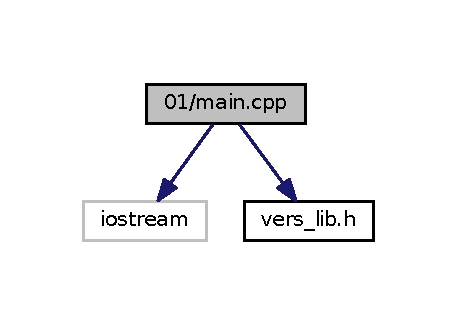
\includegraphics[width=220pt]{01_2main_8cpp__incl}
\end{center}
\end{figure}
\subsection*{Functions}
\begin{DoxyCompactItemize}
\item 
int \hyperlink{01_2main_8cpp_ae66f6b31b5ad750f1fe042a706a4e3d4}{main} ()
\end{DoxyCompactItemize}


\subsection{Function Documentation}
\index{01/main.\+cpp@{01/main.\+cpp}!main@{main}}
\index{main@{main}!01/main.\+cpp@{01/main.\+cpp}}
\subsubsection[{\texorpdfstring{main()}{main()}}]{\setlength{\rightskip}{0pt plus 5cm}int main (
\begin{DoxyParamCaption}
{}
\end{DoxyParamCaption}
)}\hypertarget{01_2main_8cpp_ae66f6b31b5ad750f1fe042a706a4e3d4}{}\label{01_2main_8cpp_ae66f6b31b5ad750f1fe042a706a4e3d4}

\hypertarget{04__sfinae_2main_8cpp}{}\section{04\+\_\+sfinae/main.cpp File Reference}
\label{04__sfinae_2main_8cpp}\index{04\+\_\+sfinae/main.\+cpp@{04\+\_\+sfinae/main.\+cpp}}
{\ttfamily \#include $<$iostream$>$}\\*
{\ttfamily \#include $<$string$>$}\\*
{\ttfamily \#include $<$map$>$}\\*
{\ttfamily \#include \char`\"{}print\+\_\+ip\+\_\+04.\+hpp\char`\"{}}\\*
Include dependency graph for main.\+cpp\+:
\nopagebreak
\begin{figure}[H]
\begin{center}
\leavevmode
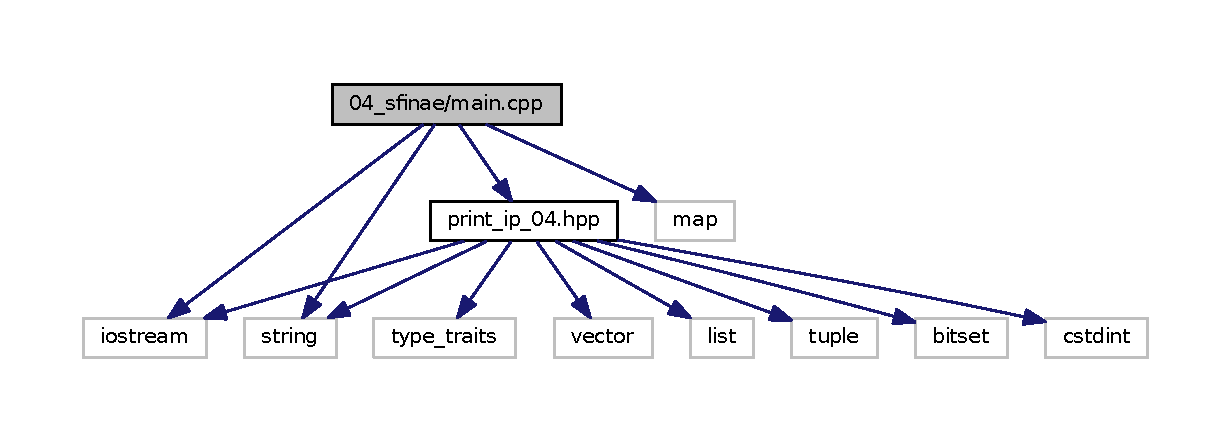
\includegraphics[width=350pt]{04__sfinae_2main_8cpp__incl}
\end{center}
\end{figure}
\subsection*{Functions}
\begin{DoxyCompactItemize}
\item 
int \hyperlink{04__sfinae_2main_8cpp_a0ddf1224851353fc92bfbff6f499fa97}{main} (int argc, char $\ast$argv\mbox{[}$\,$\mbox{]})
\end{DoxyCompactItemize}


\subsection{Function Documentation}
\index{04\+\_\+sfinae/main.\+cpp@{04\+\_\+sfinae/main.\+cpp}!main@{main}}
\index{main@{main}!04\+\_\+sfinae/main.\+cpp@{04\+\_\+sfinae/main.\+cpp}}
\subsubsection[{\texorpdfstring{main(int argc, char $\ast$argv[])}{main(int argc, char *argv[])}}]{\setlength{\rightskip}{0pt plus 5cm}int main (
\begin{DoxyParamCaption}
\item[{int}]{argc, }
\item[{char $\ast$}]{argv\mbox{[}$\,$\mbox{]}}
\end{DoxyParamCaption}
)}\hypertarget{04__sfinae_2main_8cpp_a0ddf1224851353fc92bfbff6f499fa97}{}\label{04__sfinae_2main_8cpp_a0ddf1224851353fc92bfbff6f499fa97}

\hypertarget{multithread__pc_2main_8cpp}{}\section{multithread\+\_\+pc/main.cpp File Reference}
\label{multithread__pc_2main_8cpp}\index{multithread\+\_\+pc/main.\+cpp@{multithread\+\_\+pc/main.\+cpp}}
{\ttfamily \#include \char`\"{}prod\+\_\+cons\+\_\+simulator.\+h\char`\"{}}\\*
{\ttfamily \#include $<$memory$>$}\\*
{\ttfamily \#include $<$iostream$>$}\\*
Include dependency graph for main.\+cpp\+:
\nopagebreak
\begin{figure}[H]
\begin{center}
\leavevmode
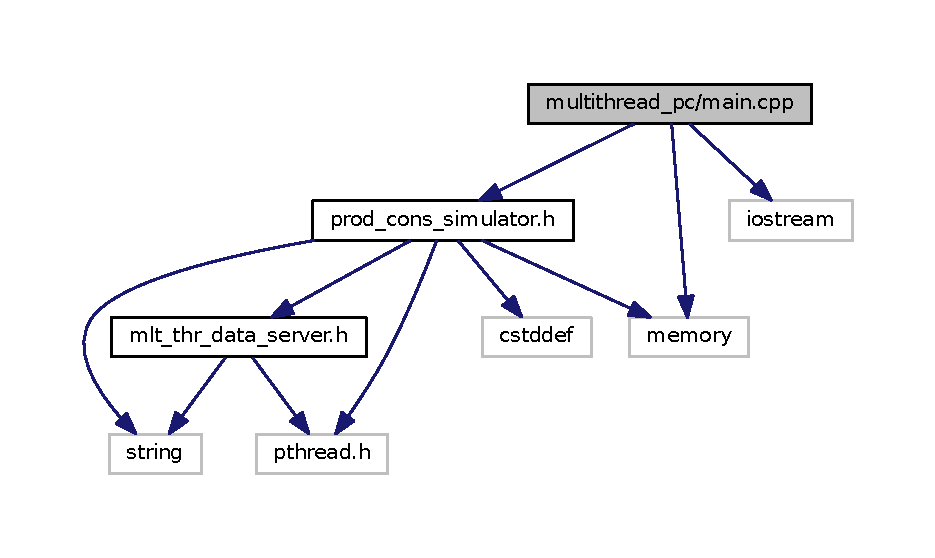
\includegraphics[width=350pt]{multithread__pc_2main_8cpp__incl}
\end{center}
\end{figure}
\subsection*{Functions}
\begin{DoxyCompactItemize}
\item 
void \hyperlink{multithread__pc_2main_8cpp_a853216ac51aa181669ff4d3de74058a7}{print\+\_\+help} ()
\item 
int \hyperlink{multithread__pc_2main_8cpp_a0ddf1224851353fc92bfbff6f499fa97}{main} (int argc, char $\ast$argv\mbox{[}$\,$\mbox{]})
\end{DoxyCompactItemize}


\subsection{Function Documentation}
\index{multithread\+\_\+pc/main.\+cpp@{multithread\+\_\+pc/main.\+cpp}!main@{main}}
\index{main@{main}!multithread\+\_\+pc/main.\+cpp@{multithread\+\_\+pc/main.\+cpp}}
\subsubsection[{\texorpdfstring{main(int argc, char $\ast$argv[])}{main(int argc, char *argv[])}}]{\setlength{\rightskip}{0pt plus 5cm}int main (
\begin{DoxyParamCaption}
\item[{int}]{argc, }
\item[{char $\ast$}]{argv\mbox{[}$\,$\mbox{]}}
\end{DoxyParamCaption}
)}\hypertarget{multithread__pc_2main_8cpp_a0ddf1224851353fc92bfbff6f499fa97}{}\label{multithread__pc_2main_8cpp_a0ddf1224851353fc92bfbff6f499fa97}
\index{multithread\+\_\+pc/main.\+cpp@{multithread\+\_\+pc/main.\+cpp}!print\+\_\+help@{print\+\_\+help}}
\index{print\+\_\+help@{print\+\_\+help}!multithread\+\_\+pc/main.\+cpp@{multithread\+\_\+pc/main.\+cpp}}
\subsubsection[{\texorpdfstring{print\+\_\+help()}{print_help()}}]{\setlength{\rightskip}{0pt plus 5cm}void print\+\_\+help (
\begin{DoxyParamCaption}
{}
\end{DoxyParamCaption}
)}\hypertarget{multithread__pc_2main_8cpp_a853216ac51aa181669ff4d3de74058a7}{}\label{multithread__pc_2main_8cpp_a853216ac51aa181669ff4d3de74058a7}

\hypertarget{test__vers__boost_8cpp}{}\section{01/test\+\_\+vers\+\_\+boost.cpp File Reference}
\label{test__vers__boost_8cpp}\index{01/test\+\_\+vers\+\_\+boost.\+cpp@{01/test\+\_\+vers\+\_\+boost.\+cpp}}
{\ttfamily \#include $<$boost/test/unit\+\_\+test.\+hpp$>$}\\*
{\ttfamily \#include \char`\"{}vers\+\_\+lib.\+h\char`\"{}}\\*
Include dependency graph for test\+\_\+vers\+\_\+boost.\+cpp\+:
\nopagebreak
\begin{figure}[H]
\begin{center}
\leavevmode
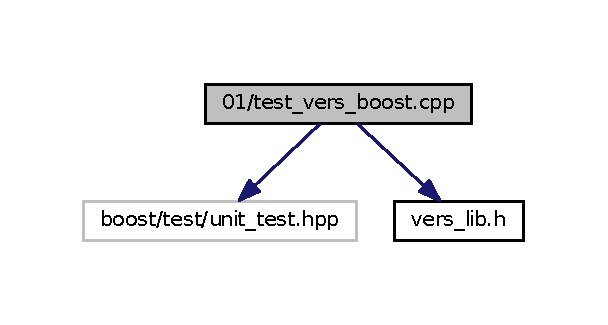
\includegraphics[width=292pt]{test__vers__boost_8cpp__incl}
\end{center}
\end{figure}
\subsection*{Macros}
\begin{DoxyCompactItemize}
\item 
\#define \hyperlink{test__vers__boost_8cpp_a6b2a3852db8bb19ab6909bac01859985}{B\+O\+O\+S\+T\+\_\+\+T\+E\+S\+T\+\_\+\+M\+O\+D\+U\+LE}~test\+\_\+vers\+\_\+boost
\end{DoxyCompactItemize}
\subsection*{Functions}
\begin{DoxyCompactItemize}
\item 
\hyperlink{test__vers__boost_8cpp_a5a8f1e117b104260d857ed534915b417}{B\+O\+O\+S\+T\+\_\+\+A\+U\+T\+O\+\_\+\+T\+E\+S\+T\+\_\+\+C\+A\+SE} (test\+\_\+valid\+\_\+version)
\end{DoxyCompactItemize}


\subsection{Macro Definition Documentation}
\index{test\+\_\+vers\+\_\+boost.\+cpp@{test\+\_\+vers\+\_\+boost.\+cpp}!B\+O\+O\+S\+T\+\_\+\+T\+E\+S\+T\+\_\+\+M\+O\+D\+U\+LE@{B\+O\+O\+S\+T\+\_\+\+T\+E\+S\+T\+\_\+\+M\+O\+D\+U\+LE}}
\index{B\+O\+O\+S\+T\+\_\+\+T\+E\+S\+T\+\_\+\+M\+O\+D\+U\+LE@{B\+O\+O\+S\+T\+\_\+\+T\+E\+S\+T\+\_\+\+M\+O\+D\+U\+LE}!test\+\_\+vers\+\_\+boost.\+cpp@{test\+\_\+vers\+\_\+boost.\+cpp}}
\subsubsection[{\texorpdfstring{B\+O\+O\+S\+T\+\_\+\+T\+E\+S\+T\+\_\+\+M\+O\+D\+U\+LE}{BOOST_TEST_MODULE}}]{\setlength{\rightskip}{0pt plus 5cm}\#define B\+O\+O\+S\+T\+\_\+\+T\+E\+S\+T\+\_\+\+M\+O\+D\+U\+LE~test\+\_\+vers\+\_\+boost}\hypertarget{test__vers__boost_8cpp_a6b2a3852db8bb19ab6909bac01859985}{}\label{test__vers__boost_8cpp_a6b2a3852db8bb19ab6909bac01859985}


\subsection{Function Documentation}
\index{test\+\_\+vers\+\_\+boost.\+cpp@{test\+\_\+vers\+\_\+boost.\+cpp}!B\+O\+O\+S\+T\+\_\+\+A\+U\+T\+O\+\_\+\+T\+E\+S\+T\+\_\+\+C\+A\+SE@{B\+O\+O\+S\+T\+\_\+\+A\+U\+T\+O\+\_\+\+T\+E\+S\+T\+\_\+\+C\+A\+SE}}
\index{B\+O\+O\+S\+T\+\_\+\+A\+U\+T\+O\+\_\+\+T\+E\+S\+T\+\_\+\+C\+A\+SE@{B\+O\+O\+S\+T\+\_\+\+A\+U\+T\+O\+\_\+\+T\+E\+S\+T\+\_\+\+C\+A\+SE}!test\+\_\+vers\+\_\+boost.\+cpp@{test\+\_\+vers\+\_\+boost.\+cpp}}
\subsubsection[{\texorpdfstring{B\+O\+O\+S\+T\+\_\+\+A\+U\+T\+O\+\_\+\+T\+E\+S\+T\+\_\+\+C\+A\+S\+E(test\+\_\+valid\+\_\+version)}{BOOST_AUTO_TEST_CASE(test_valid_version)}}]{\setlength{\rightskip}{0pt plus 5cm}B\+O\+O\+S\+T\+\_\+\+A\+U\+T\+O\+\_\+\+T\+E\+S\+T\+\_\+\+C\+A\+SE (
\begin{DoxyParamCaption}
\item[{test\+\_\+valid\+\_\+version}]{}
\end{DoxyParamCaption}
)}\hypertarget{test__vers__boost_8cpp_a5a8f1e117b104260d857ed534915b417}{}\label{test__vers__boost_8cpp_a5a8f1e117b104260d857ed534915b417}

\hypertarget{test__vers__gtest_8cpp}{}\section{01/test\+\_\+vers\+\_\+gtest.cpp File Reference}
\label{test__vers__gtest_8cpp}\index{01/test\+\_\+vers\+\_\+gtest.\+cpp@{01/test\+\_\+vers\+\_\+gtest.\+cpp}}
{\ttfamily \#include $<$gtest/gtest.\+h$>$}\\*
{\ttfamily \#include \char`\"{}vers\+\_\+lib.\+h\char`\"{}}\\*
Include dependency graph for test\+\_\+vers\+\_\+gtest.\+cpp\+:
\nopagebreak
\begin{figure}[H]
\begin{center}
\leavevmode
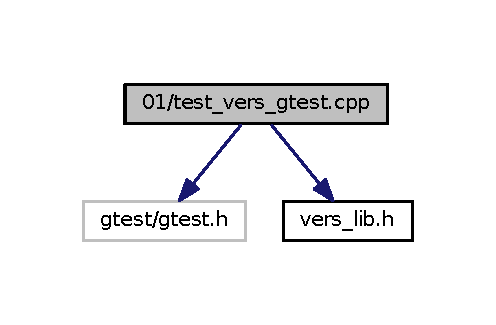
\includegraphics[width=238pt]{test__vers__gtest_8cpp__incl}
\end{center}
\end{figure}
\subsection*{Functions}
\begin{DoxyCompactItemize}
\item 
\hyperlink{test__vers__gtest_8cpp_ad040b370b89121e8a68bf66636367f02}{T\+E\+ST} (test\+\_\+vers\+\_\+gtest, valid\+\_\+versions)
\item 
int \hyperlink{test__vers__gtest_8cpp_a0ddf1224851353fc92bfbff6f499fa97}{main} (int argc, char $\ast$argv\mbox{[}$\,$\mbox{]})
\end{DoxyCompactItemize}


\subsection{Function Documentation}
\index{test\+\_\+vers\+\_\+gtest.\+cpp@{test\+\_\+vers\+\_\+gtest.\+cpp}!main@{main}}
\index{main@{main}!test\+\_\+vers\+\_\+gtest.\+cpp@{test\+\_\+vers\+\_\+gtest.\+cpp}}
\subsubsection[{\texorpdfstring{main(int argc, char $\ast$argv[])}{main(int argc, char *argv[])}}]{\setlength{\rightskip}{0pt plus 5cm}int main (
\begin{DoxyParamCaption}
\item[{int}]{argc, }
\item[{char $\ast$}]{argv\mbox{[}$\,$\mbox{]}}
\end{DoxyParamCaption}
)}\hypertarget{test__vers__gtest_8cpp_a0ddf1224851353fc92bfbff6f499fa97}{}\label{test__vers__gtest_8cpp_a0ddf1224851353fc92bfbff6f499fa97}
\index{test\+\_\+vers\+\_\+gtest.\+cpp@{test\+\_\+vers\+\_\+gtest.\+cpp}!T\+E\+ST@{T\+E\+ST}}
\index{T\+E\+ST@{T\+E\+ST}!test\+\_\+vers\+\_\+gtest.\+cpp@{test\+\_\+vers\+\_\+gtest.\+cpp}}
\subsubsection[{\texorpdfstring{T\+E\+S\+T(test\+\_\+vers\+\_\+gtest, valid\+\_\+versions)}{TEST(test_vers_gtest, valid_versions)}}]{\setlength{\rightskip}{0pt plus 5cm}T\+E\+ST (
\begin{DoxyParamCaption}
\item[{test\+\_\+vers\+\_\+gtest}]{, }
\item[{valid\+\_\+versions}]{}
\end{DoxyParamCaption}
)}\hypertarget{test__vers__gtest_8cpp_ad040b370b89121e8a68bf66636367f02}{}\label{test__vers__gtest_8cpp_ad040b370b89121e8a68bf66636367f02}

\hypertarget{vers__lib_8cpp}{}\section{01/vers\+\_\+lib.cpp File Reference}
\label{vers__lib_8cpp}\index{01/vers\+\_\+lib.\+cpp@{01/vers\+\_\+lib.\+cpp}}
{\ttfamily \#include \char`\"{}vers\+\_\+lib.\+h\char`\"{}}\\*
{\ttfamily \#include \char`\"{}version.\+h\char`\"{}}\\*
Include dependency graph for vers\+\_\+lib.\+cpp\+:
\nopagebreak
\begin{figure}[H]
\begin{center}
\leavevmode
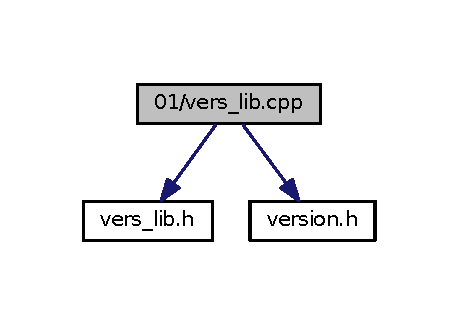
\includegraphics[width=220pt]{vers__lib_8cpp__incl}
\end{center}
\end{figure}
\subsection*{Functions}
\begin{DoxyCompactItemize}
\item 
int \hyperlink{vers__lib_8cpp_aa9387ddec2c78390f4fdf3b979348d62}{version\+\_\+major} () noexcept
\item 
int \hyperlink{vers__lib_8cpp_a5de5ba4c90576bf63ff2d44a821feb48}{version\+\_\+minor} () noexcept
\item 
int \hyperlink{vers__lib_8cpp_ac2c281eb9fc0ae960c904d8f7dfd082c}{version\+\_\+patch} () noexcept
\end{DoxyCompactItemize}


\subsection{Function Documentation}
\index{vers\+\_\+lib.\+cpp@{vers\+\_\+lib.\+cpp}!version\+\_\+major@{version\+\_\+major}}
\index{version\+\_\+major@{version\+\_\+major}!vers\+\_\+lib.\+cpp@{vers\+\_\+lib.\+cpp}}
\subsubsection[{\texorpdfstring{version\+\_\+major() noexcept}{version_major() noexcept}}]{\setlength{\rightskip}{0pt plus 5cm}int version\+\_\+major (
\begin{DoxyParamCaption}
{}
\end{DoxyParamCaption}
)\hspace{0.3cm}{\ttfamily [noexcept]}}\hypertarget{vers__lib_8cpp_aa9387ddec2c78390f4fdf3b979348d62}{}\label{vers__lib_8cpp_aa9387ddec2c78390f4fdf3b979348d62}
\index{vers\+\_\+lib.\+cpp@{vers\+\_\+lib.\+cpp}!version\+\_\+minor@{version\+\_\+minor}}
\index{version\+\_\+minor@{version\+\_\+minor}!vers\+\_\+lib.\+cpp@{vers\+\_\+lib.\+cpp}}
\subsubsection[{\texorpdfstring{version\+\_\+minor() noexcept}{version_minor() noexcept}}]{\setlength{\rightskip}{0pt plus 5cm}int version\+\_\+minor (
\begin{DoxyParamCaption}
{}
\end{DoxyParamCaption}
)\hspace{0.3cm}{\ttfamily [noexcept]}}\hypertarget{vers__lib_8cpp_a5de5ba4c90576bf63ff2d44a821feb48}{}\label{vers__lib_8cpp_a5de5ba4c90576bf63ff2d44a821feb48}
\index{vers\+\_\+lib.\+cpp@{vers\+\_\+lib.\+cpp}!version\+\_\+patch@{version\+\_\+patch}}
\index{version\+\_\+patch@{version\+\_\+patch}!vers\+\_\+lib.\+cpp@{vers\+\_\+lib.\+cpp}}
\subsubsection[{\texorpdfstring{version\+\_\+patch() noexcept}{version_patch() noexcept}}]{\setlength{\rightskip}{0pt plus 5cm}int version\+\_\+patch (
\begin{DoxyParamCaption}
{}
\end{DoxyParamCaption}
)\hspace{0.3cm}{\ttfamily [noexcept]}}\hypertarget{vers__lib_8cpp_ac2c281eb9fc0ae960c904d8f7dfd082c}{}\label{vers__lib_8cpp_ac2c281eb9fc0ae960c904d8f7dfd082c}

\hypertarget{vers__lib_8h}{}\section{01/vers\+\_\+lib.h File Reference}
\label{vers__lib_8h}\index{01/vers\+\_\+lib.\+h@{01/vers\+\_\+lib.\+h}}
This graph shows which files directly or indirectly include this file\+:
\nopagebreak
\begin{figure}[H]
\begin{center}
\leavevmode
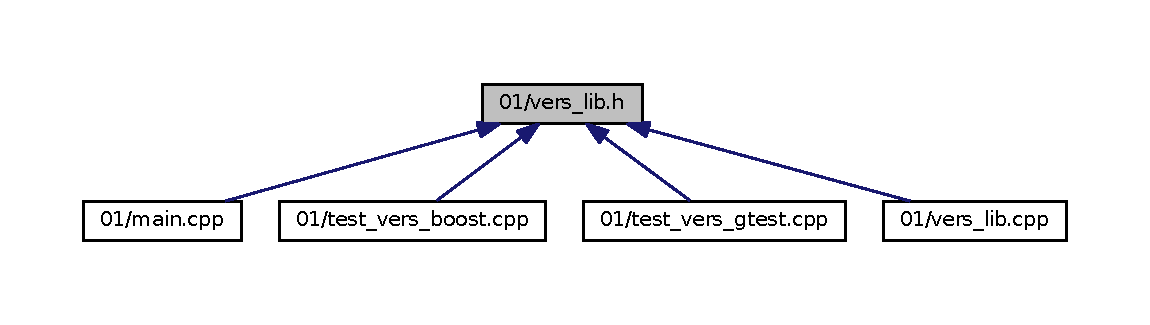
\includegraphics[width=350pt]{vers__lib_8h__dep__incl}
\end{center}
\end{figure}
\subsection*{Functions}
\begin{DoxyCompactItemize}
\item 
int \hyperlink{vers__lib_8h_aa9387ddec2c78390f4fdf3b979348d62}{version\+\_\+major} () noexcept
\item 
int \hyperlink{vers__lib_8h_a5de5ba4c90576bf63ff2d44a821feb48}{version\+\_\+minor} () noexcept
\item 
int \hyperlink{vers__lib_8h_ac2c281eb9fc0ae960c904d8f7dfd082c}{version\+\_\+patch} () noexcept
\end{DoxyCompactItemize}


\subsection{Function Documentation}
\index{vers\+\_\+lib.\+h@{vers\+\_\+lib.\+h}!version\+\_\+major@{version\+\_\+major}}
\index{version\+\_\+major@{version\+\_\+major}!vers\+\_\+lib.\+h@{vers\+\_\+lib.\+h}}
\subsubsection[{\texorpdfstring{version\+\_\+major() noexcept}{version_major() noexcept}}]{\setlength{\rightskip}{0pt plus 5cm}int version\+\_\+major (
\begin{DoxyParamCaption}
{}
\end{DoxyParamCaption}
)\hspace{0.3cm}{\ttfamily [noexcept]}}\hypertarget{vers__lib_8h_aa9387ddec2c78390f4fdf3b979348d62}{}\label{vers__lib_8h_aa9387ddec2c78390f4fdf3b979348d62}
\index{vers\+\_\+lib.\+h@{vers\+\_\+lib.\+h}!version\+\_\+minor@{version\+\_\+minor}}
\index{version\+\_\+minor@{version\+\_\+minor}!vers\+\_\+lib.\+h@{vers\+\_\+lib.\+h}}
\subsubsection[{\texorpdfstring{version\+\_\+minor() noexcept}{version_minor() noexcept}}]{\setlength{\rightskip}{0pt plus 5cm}int version\+\_\+minor (
\begin{DoxyParamCaption}
{}
\end{DoxyParamCaption}
)\hspace{0.3cm}{\ttfamily [noexcept]}}\hypertarget{vers__lib_8h_a5de5ba4c90576bf63ff2d44a821feb48}{}\label{vers__lib_8h_a5de5ba4c90576bf63ff2d44a821feb48}
\index{vers\+\_\+lib.\+h@{vers\+\_\+lib.\+h}!version\+\_\+patch@{version\+\_\+patch}}
\index{version\+\_\+patch@{version\+\_\+patch}!vers\+\_\+lib.\+h@{vers\+\_\+lib.\+h}}
\subsubsection[{\texorpdfstring{version\+\_\+patch() noexcept}{version_patch() noexcept}}]{\setlength{\rightskip}{0pt plus 5cm}int version\+\_\+patch (
\begin{DoxyParamCaption}
{}
\end{DoxyParamCaption}
)\hspace{0.3cm}{\ttfamily [noexcept]}}\hypertarget{vers__lib_8h_ac2c281eb9fc0ae960c904d8f7dfd082c}{}\label{vers__lib_8h_ac2c281eb9fc0ae960c904d8f7dfd082c}

\hypertarget{version_8h}{}\section{01/version.h File Reference}
\label{version_8h}\index{01/version.\+h@{01/version.\+h}}
This graph shows which files directly or indirectly include this file\+:
\nopagebreak
\begin{figure}[H]
\begin{center}
\leavevmode
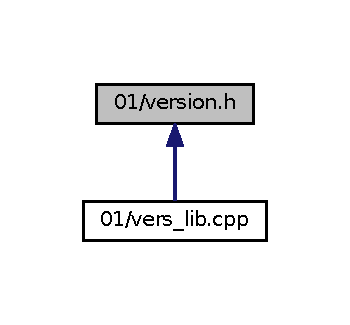
\includegraphics[width=168pt]{version_8h__dep__incl}
\end{center}
\end{figure}
\subsection*{Macros}
\begin{DoxyCompactItemize}
\item 
\#define \hyperlink{version_8h_a4a5fc96a4bdd7d68ed99ccce9ca2e77e}{P\+R\+O\+J\+E\+C\+T\+\_\+\+V\+E\+R\+S\+I\+O\+N\+\_\+\+P\+A\+T\+CH}~1
\item 
\#define \hyperlink{version_8h_a43e23009192a3e216fefec17750d8673}{P\+R\+O\+J\+E\+C\+T\+\_\+\+V\+E\+R\+S\+I\+O\+N\+\_\+\+M\+I\+N\+OR}~0
\item 
\#define \hyperlink{version_8h_abecd2198575b690d25a741857f8390d1}{P\+R\+O\+J\+E\+C\+T\+\_\+\+V\+E\+R\+S\+I\+O\+N\+\_\+\+M\+A\+J\+OR}~0
\end{DoxyCompactItemize}


\subsection{Macro Definition Documentation}
\index{version.\+h@{version.\+h}!P\+R\+O\+J\+E\+C\+T\+\_\+\+V\+E\+R\+S\+I\+O\+N\+\_\+\+M\+A\+J\+OR@{P\+R\+O\+J\+E\+C\+T\+\_\+\+V\+E\+R\+S\+I\+O\+N\+\_\+\+M\+A\+J\+OR}}
\index{P\+R\+O\+J\+E\+C\+T\+\_\+\+V\+E\+R\+S\+I\+O\+N\+\_\+\+M\+A\+J\+OR@{P\+R\+O\+J\+E\+C\+T\+\_\+\+V\+E\+R\+S\+I\+O\+N\+\_\+\+M\+A\+J\+OR}!version.\+h@{version.\+h}}
\subsubsection[{\texorpdfstring{P\+R\+O\+J\+E\+C\+T\+\_\+\+V\+E\+R\+S\+I\+O\+N\+\_\+\+M\+A\+J\+OR}{PROJECT_VERSION_MAJOR}}]{\setlength{\rightskip}{0pt plus 5cm}\#define P\+R\+O\+J\+E\+C\+T\+\_\+\+V\+E\+R\+S\+I\+O\+N\+\_\+\+M\+A\+J\+OR~0}\hypertarget{version_8h_abecd2198575b690d25a741857f8390d1}{}\label{version_8h_abecd2198575b690d25a741857f8390d1}
\index{version.\+h@{version.\+h}!P\+R\+O\+J\+E\+C\+T\+\_\+\+V\+E\+R\+S\+I\+O\+N\+\_\+\+M\+I\+N\+OR@{P\+R\+O\+J\+E\+C\+T\+\_\+\+V\+E\+R\+S\+I\+O\+N\+\_\+\+M\+I\+N\+OR}}
\index{P\+R\+O\+J\+E\+C\+T\+\_\+\+V\+E\+R\+S\+I\+O\+N\+\_\+\+M\+I\+N\+OR@{P\+R\+O\+J\+E\+C\+T\+\_\+\+V\+E\+R\+S\+I\+O\+N\+\_\+\+M\+I\+N\+OR}!version.\+h@{version.\+h}}
\subsubsection[{\texorpdfstring{P\+R\+O\+J\+E\+C\+T\+\_\+\+V\+E\+R\+S\+I\+O\+N\+\_\+\+M\+I\+N\+OR}{PROJECT_VERSION_MINOR}}]{\setlength{\rightskip}{0pt plus 5cm}\#define P\+R\+O\+J\+E\+C\+T\+\_\+\+V\+E\+R\+S\+I\+O\+N\+\_\+\+M\+I\+N\+OR~0}\hypertarget{version_8h_a43e23009192a3e216fefec17750d8673}{}\label{version_8h_a43e23009192a3e216fefec17750d8673}
\index{version.\+h@{version.\+h}!P\+R\+O\+J\+E\+C\+T\+\_\+\+V\+E\+R\+S\+I\+O\+N\+\_\+\+P\+A\+T\+CH@{P\+R\+O\+J\+E\+C\+T\+\_\+\+V\+E\+R\+S\+I\+O\+N\+\_\+\+P\+A\+T\+CH}}
\index{P\+R\+O\+J\+E\+C\+T\+\_\+\+V\+E\+R\+S\+I\+O\+N\+\_\+\+P\+A\+T\+CH@{P\+R\+O\+J\+E\+C\+T\+\_\+\+V\+E\+R\+S\+I\+O\+N\+\_\+\+P\+A\+T\+CH}!version.\+h@{version.\+h}}
\subsubsection[{\texorpdfstring{P\+R\+O\+J\+E\+C\+T\+\_\+\+V\+E\+R\+S\+I\+O\+N\+\_\+\+P\+A\+T\+CH}{PROJECT_VERSION_PATCH}}]{\setlength{\rightskip}{0pt plus 5cm}\#define P\+R\+O\+J\+E\+C\+T\+\_\+\+V\+E\+R\+S\+I\+O\+N\+\_\+\+P\+A\+T\+CH~1}\hypertarget{version_8h_a4a5fc96a4bdd7d68ed99ccce9ca2e77e}{}\label{version_8h_a4a5fc96a4bdd7d68ed99ccce9ca2e77e}

\hypertarget{constexpr__func_8cpp}{}\section{02/constexpr\+\_\+func.cpp File Reference}
\label{constexpr__func_8cpp}\index{02/constexpr\+\_\+func.\+cpp@{02/constexpr\+\_\+func.\+cpp}}
{\ttfamily \#include $<$cstddef$>$}\\*
Include dependency graph for constexpr\+\_\+func.\+cpp\+:
\nopagebreak
\begin{figure}[H]
\begin{center}
\leavevmode
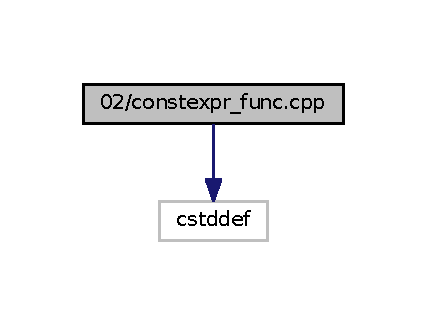
\includegraphics[width=205pt]{constexpr__func_8cpp__incl}
\end{center}
\end{figure}
\subsection*{Functions}
\begin{DoxyCompactItemize}
\item 
constexpr size\+\_\+t \hyperlink{constexpr__func_8cpp_ac1bdbb03b521f0a895628c2fd7d3b650}{bin\+\_\+id\+\_\+gt\+\_\+1} (size\+\_\+t x)
\item 
constexpr size\+\_\+t \hyperlink{constexpr__func_8cpp_a5064165737191e9f5069e4782a7e9a7b}{bin\+\_\+id} (size\+\_\+t x)
\item 
int \hyperlink{constexpr__func_8cpp_a0ddf1224851353fc92bfbff6f499fa97}{main} (int argc, char $\ast$argv\mbox{[}$\,$\mbox{]})
\end{DoxyCompactItemize}


\subsection{Function Documentation}
\index{constexpr\+\_\+func.\+cpp@{constexpr\+\_\+func.\+cpp}!bin\+\_\+id@{bin\+\_\+id}}
\index{bin\+\_\+id@{bin\+\_\+id}!constexpr\+\_\+func.\+cpp@{constexpr\+\_\+func.\+cpp}}
\subsubsection[{\texorpdfstring{bin\+\_\+id(size\+\_\+t x)}{bin_id(size_t x)}}]{\setlength{\rightskip}{0pt plus 5cm}constexpr size\+\_\+t bin\+\_\+id (
\begin{DoxyParamCaption}
\item[{size\+\_\+t}]{x}
\end{DoxyParamCaption}
)}\hypertarget{constexpr__func_8cpp_a5064165737191e9f5069e4782a7e9a7b}{}\label{constexpr__func_8cpp_a5064165737191e9f5069e4782a7e9a7b}
\index{constexpr\+\_\+func.\+cpp@{constexpr\+\_\+func.\+cpp}!bin\+\_\+id\+\_\+gt\+\_\+1@{bin\+\_\+id\+\_\+gt\+\_\+1}}
\index{bin\+\_\+id\+\_\+gt\+\_\+1@{bin\+\_\+id\+\_\+gt\+\_\+1}!constexpr\+\_\+func.\+cpp@{constexpr\+\_\+func.\+cpp}}
\subsubsection[{\texorpdfstring{bin\+\_\+id\+\_\+gt\+\_\+1(size\+\_\+t x)}{bin_id_gt_1(size_t x)}}]{\setlength{\rightskip}{0pt plus 5cm}constexpr size\+\_\+t bin\+\_\+id\+\_\+gt\+\_\+1 (
\begin{DoxyParamCaption}
\item[{size\+\_\+t}]{x}
\end{DoxyParamCaption}
)}\hypertarget{constexpr__func_8cpp_ac1bdbb03b521f0a895628c2fd7d3b650}{}\label{constexpr__func_8cpp_ac1bdbb03b521f0a895628c2fd7d3b650}
\index{constexpr\+\_\+func.\+cpp@{constexpr\+\_\+func.\+cpp}!main@{main}}
\index{main@{main}!constexpr\+\_\+func.\+cpp@{constexpr\+\_\+func.\+cpp}}
\subsubsection[{\texorpdfstring{main(int argc, char $\ast$argv[])}{main(int argc, char *argv[])}}]{\setlength{\rightskip}{0pt plus 5cm}int main (
\begin{DoxyParamCaption}
\item[{int}]{argc, }
\item[{char $\ast$}]{argv\mbox{[}$\,$\mbox{]}}
\end{DoxyParamCaption}
)}\hypertarget{constexpr__func_8cpp_a0ddf1224851353fc92bfbff6f499fa97}{}\label{constexpr__func_8cpp_a0ddf1224851353fc92bfbff6f499fa97}

\hypertarget{02_2ip__loader_8cpp}{}\section{02/ip\+\_\+loader.cpp File Reference}
\label{02_2ip__loader_8cpp}\index{02/ip\+\_\+loader.\+cpp@{02/ip\+\_\+loader.\+cpp}}
{\ttfamily \#include \char`\"{}ip\+\_\+loader.\+h\char`\"{}}\\*
{\ttfamily \#include $<$iostream$>$}\\*
Include dependency graph for ip\+\_\+loader.\+cpp\+:
\nopagebreak
\begin{figure}[H]
\begin{center}
\leavevmode
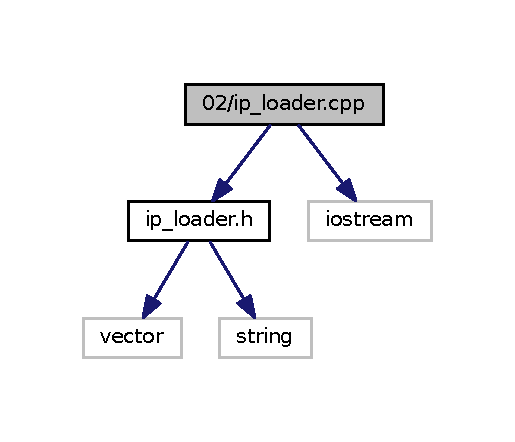
\includegraphics[width=247pt]{02_2ip__loader_8cpp__incl}
\end{center}
\end{figure}

\hypertarget{03__ranges_2ip__loader_8cpp}{}\section{03\+\_\+ranges/ip\+\_\+loader.cpp File Reference}
\label{03__ranges_2ip__loader_8cpp}\index{03\+\_\+ranges/ip\+\_\+loader.\+cpp@{03\+\_\+ranges/ip\+\_\+loader.\+cpp}}
{\ttfamily \#include \char`\"{}ip\+\_\+loader.\+h\char`\"{}}\\*
{\ttfamily \#include $<$iostream$>$}\\*
{\ttfamily \#include $<$vector$>$}\\*
{\ttfamily \#include $<$string$>$}\\*
{\ttfamily \#include $<$meta/meta.\+hpp$>$}\\*
{\ttfamily \#include $<$range/v3/algorithm/sort.\+hpp$>$}\\*
{\ttfamily \#include $<$range/v3/all.\+hpp$>$}\\*
{\ttfamily \#include $<$range/v3/algorithm.\+hpp$>$}\\*
{\ttfamily \#include $<$range/v3/iterator.\+hpp$>$}\\*
{\ttfamily \#include $<$range/v3/view/split.\+hpp$>$}\\*
Include dependency graph for ip\+\_\+loader.\+cpp\+:
\nopagebreak
\begin{figure}[H]
\begin{center}
\leavevmode
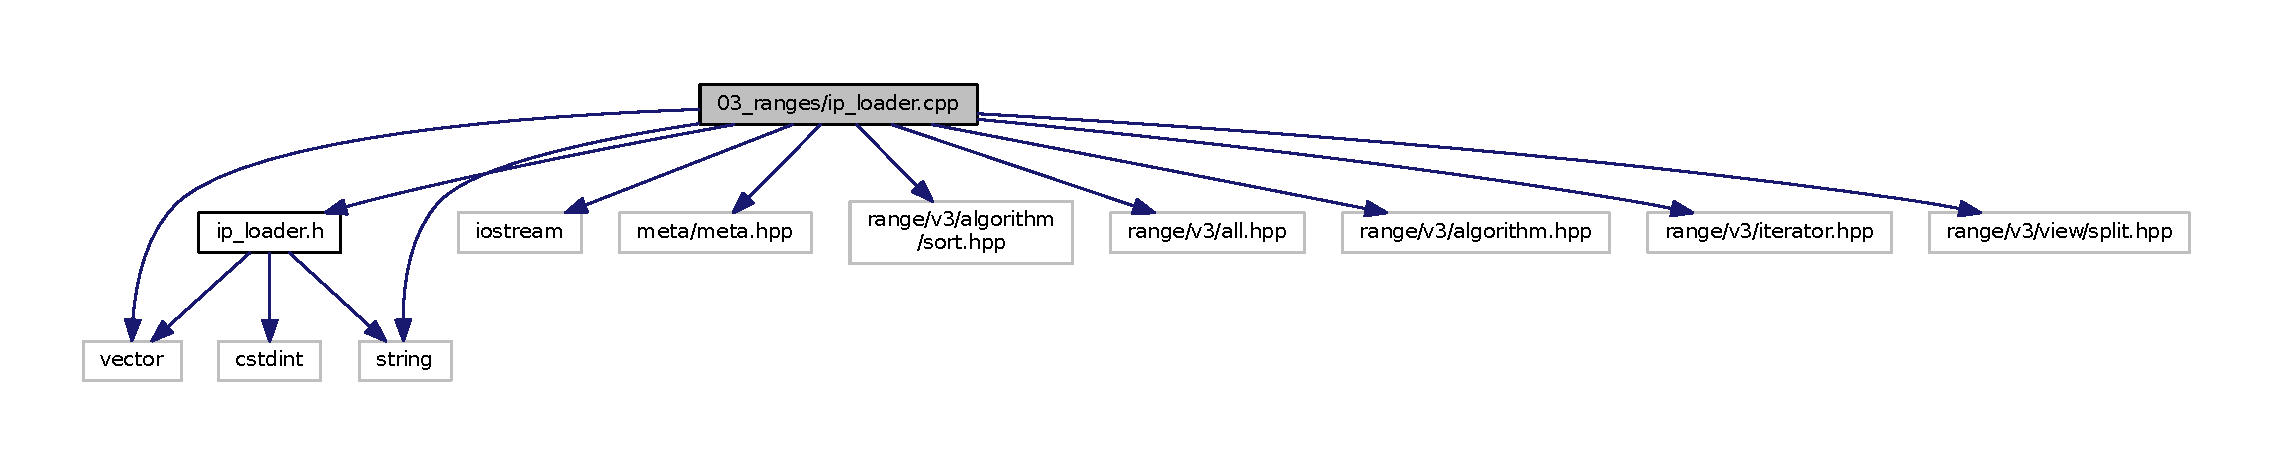
\includegraphics[width=350pt]{03__ranges_2ip__loader_8cpp__incl}
\end{center}
\end{figure}

\hypertarget{02_2ip__loader_8h}{}\section{02/ip\+\_\+loader.h File Reference}
\label{02_2ip__loader_8h}\index{02/ip\+\_\+loader.\+h@{02/ip\+\_\+loader.\+h}}
{\ttfamily \#include $<$vector$>$}\\*
{\ttfamily \#include $<$string$>$}\\*
Include dependency graph for ip\+\_\+loader.\+h\+:
\nopagebreak
\begin{figure}[H]
\begin{center}
\leavevmode
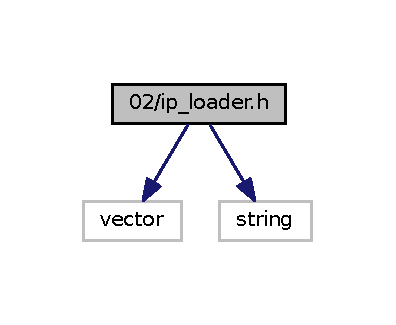
\includegraphics[width=190pt]{02_2ip__loader_8h__incl}
\end{center}
\end{figure}
This graph shows which files directly or indirectly include this file\+:
\nopagebreak
\begin{figure}[H]
\begin{center}
\leavevmode
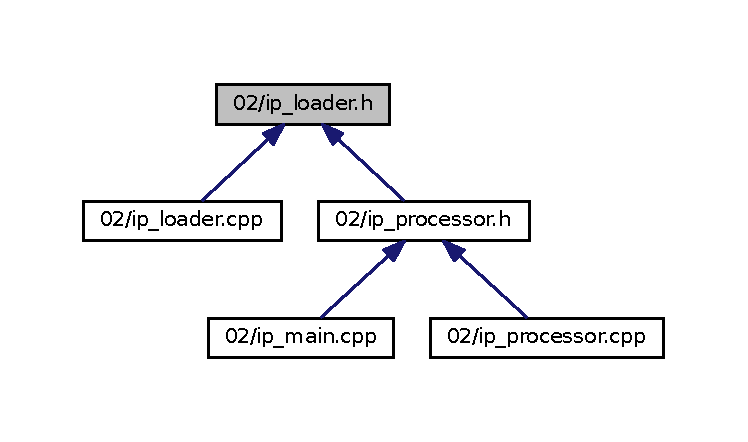
\includegraphics[width=350pt]{02_2ip__loader_8h__dep__incl}
\end{center}
\end{figure}
\subsection*{Classes}
\begin{DoxyCompactItemize}
\item 
class \hyperlink{classIpDataLoader}{Ip\+Data\+Loader}
\end{DoxyCompactItemize}
\subsection*{Typedefs}
\begin{DoxyCompactItemize}
\item 
using \hyperlink{02_2ip__loader_8h_ad6543533a9d8728e8ffbb208890f492e}{vec\+\_\+str} = vector$<$ string $>$
\end{DoxyCompactItemize}


\subsection{Typedef Documentation}
\index{02/ip\+\_\+loader.\+h@{02/ip\+\_\+loader.\+h}!vec\+\_\+str@{vec\+\_\+str}}
\index{vec\+\_\+str@{vec\+\_\+str}!02/ip\+\_\+loader.\+h@{02/ip\+\_\+loader.\+h}}
\subsubsection[{\texorpdfstring{vec\+\_\+str}{vec_str}}]{\setlength{\rightskip}{0pt plus 5cm}using {\bf vec\+\_\+str} =  vector$<$string$>$}\hypertarget{02_2ip__loader_8h_ad6543533a9d8728e8ffbb208890f492e}{}\label{02_2ip__loader_8h_ad6543533a9d8728e8ffbb208890f492e}

\hypertarget{03__ranges_2ip__loader_8h}{}\section{03\+\_\+ranges/ip\+\_\+loader.h File Reference}
\label{03__ranges_2ip__loader_8h}\index{03\+\_\+ranges/ip\+\_\+loader.\+h@{03\+\_\+ranges/ip\+\_\+loader.\+h}}
{\ttfamily \#include $<$vector$>$}\\*
{\ttfamily \#include $<$string$>$}\\*
{\ttfamily \#include $<$cstdint$>$}\\*
Include dependency graph for ip\+\_\+loader.\+h\+:
\nopagebreak
\begin{figure}[H]
\begin{center}
\leavevmode
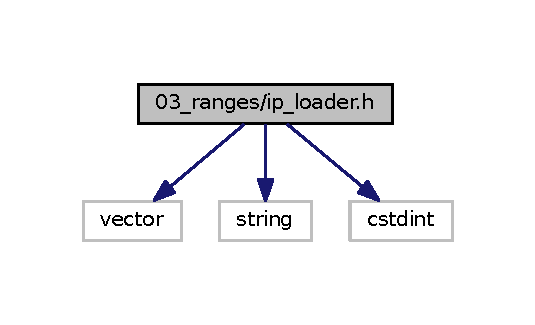
\includegraphics[width=257pt]{03__ranges_2ip__loader_8h__incl}
\end{center}
\end{figure}
This graph shows which files directly or indirectly include this file\+:
\nopagebreak
\begin{figure}[H]
\begin{center}
\leavevmode
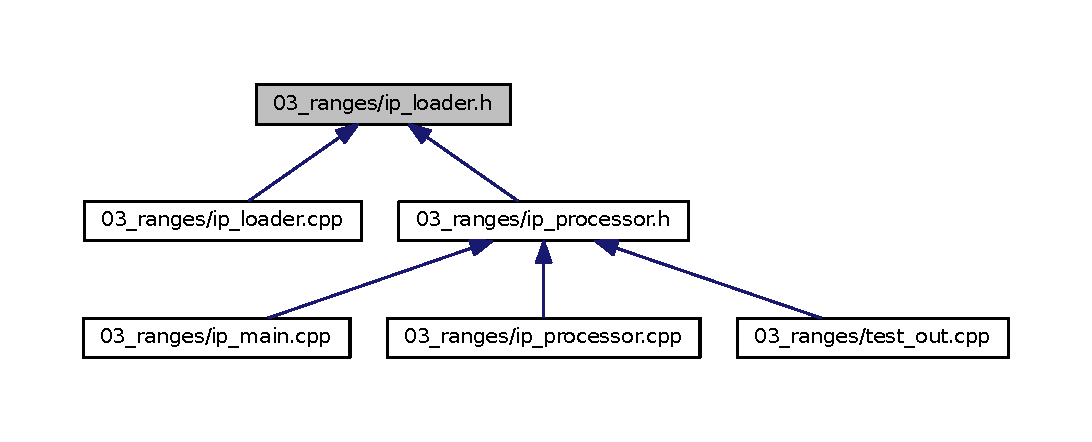
\includegraphics[width=350pt]{03__ranges_2ip__loader_8h__dep__incl}
\end{center}
\end{figure}
\subsection*{Classes}
\begin{DoxyCompactItemize}
\item 
class \hyperlink{classIpDataLoader}{Ip\+Data\+Loader}
\end{DoxyCompactItemize}
\subsection*{Typedefs}
\begin{DoxyCompactItemize}
\item 
using \hyperlink{03__ranges_2ip__loader_8h_adf9c1fa121650f19b895ecb6217615f2}{vec\+\_\+ui8} = vector$<$ uint8\+\_\+t $>$
\end{DoxyCompactItemize}


\subsection{Typedef Documentation}
\index{03\+\_\+ranges/ip\+\_\+loader.\+h@{03\+\_\+ranges/ip\+\_\+loader.\+h}!vec\+\_\+ui8@{vec\+\_\+ui8}}
\index{vec\+\_\+ui8@{vec\+\_\+ui8}!03\+\_\+ranges/ip\+\_\+loader.\+h@{03\+\_\+ranges/ip\+\_\+loader.\+h}}
\subsubsection[{\texorpdfstring{vec\+\_\+ui8}{vec_ui8}}]{\setlength{\rightskip}{0pt plus 5cm}using {\bf vec\+\_\+ui8} =  vector$<$uint8\+\_\+t$>$}\hypertarget{03__ranges_2ip__loader_8h_adf9c1fa121650f19b895ecb6217615f2}{}\label{03__ranges_2ip__loader_8h_adf9c1fa121650f19b895ecb6217615f2}

\hypertarget{02_2ip__main_8cpp}{}\section{02/ip\+\_\+main.cpp File Reference}
\label{02_2ip__main_8cpp}\index{02/ip\+\_\+main.\+cpp@{02/ip\+\_\+main.\+cpp}}
{\ttfamily \#include \char`\"{}ip\+\_\+processor.\+h\char`\"{}}\\*
{\ttfamily \#include $<$iostream$>$}\\*
{\ttfamily \#include $<$memory$>$}\\*
Include dependency graph for ip\+\_\+main.\+cpp\+:
\nopagebreak
\begin{figure}[H]
\begin{center}
\leavevmode
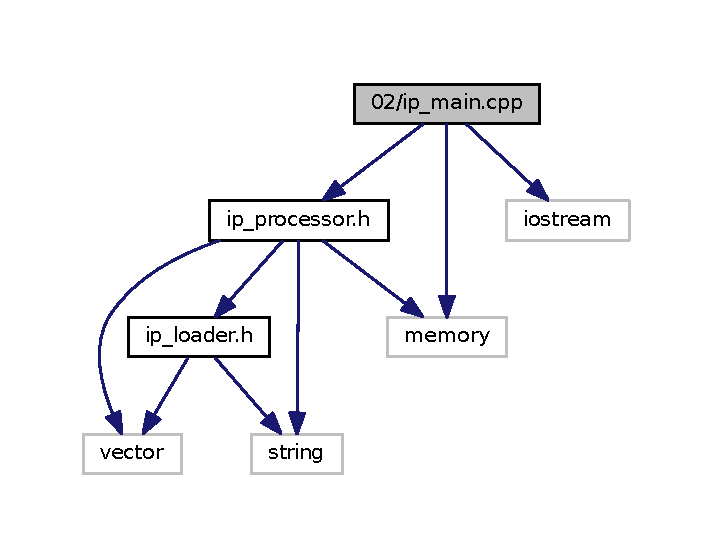
\includegraphics[width=342pt]{02_2ip__main_8cpp__incl}
\end{center}
\end{figure}
\subsection*{Functions}
\begin{DoxyCompactItemize}
\item 
int \hyperlink{02_2ip__main_8cpp_a0ddf1224851353fc92bfbff6f499fa97}{main} (int argc, char $\ast$argv\mbox{[}$\,$\mbox{]})
\end{DoxyCompactItemize}


\subsection{Function Documentation}
\index{02/ip\+\_\+main.\+cpp@{02/ip\+\_\+main.\+cpp}!main@{main}}
\index{main@{main}!02/ip\+\_\+main.\+cpp@{02/ip\+\_\+main.\+cpp}}
\subsubsection[{\texorpdfstring{main(int argc, char $\ast$argv[])}{main(int argc, char *argv[])}}]{\setlength{\rightskip}{0pt plus 5cm}int main (
\begin{DoxyParamCaption}
\item[{int}]{argc, }
\item[{char $\ast$}]{argv\mbox{[}$\,$\mbox{]}}
\end{DoxyParamCaption}
)}\hypertarget{02_2ip__main_8cpp_a0ddf1224851353fc92bfbff6f499fa97}{}\label{02_2ip__main_8cpp_a0ddf1224851353fc92bfbff6f499fa97}

\hypertarget{03__ranges_2ip__main_8cpp}{}\section{03\+\_\+ranges/ip\+\_\+main.cpp File Reference}
\label{03__ranges_2ip__main_8cpp}\index{03\+\_\+ranges/ip\+\_\+main.\+cpp@{03\+\_\+ranges/ip\+\_\+main.\+cpp}}
{\ttfamily \#include \char`\"{}ip\+\_\+processor.\+h\char`\"{}}\\*
{\ttfamily \#include $<$iostream$>$}\\*
{\ttfamily \#include $<$memory$>$}\\*
Include dependency graph for ip\+\_\+main.\+cpp\+:
\nopagebreak
\begin{figure}[H]
\begin{center}
\leavevmode
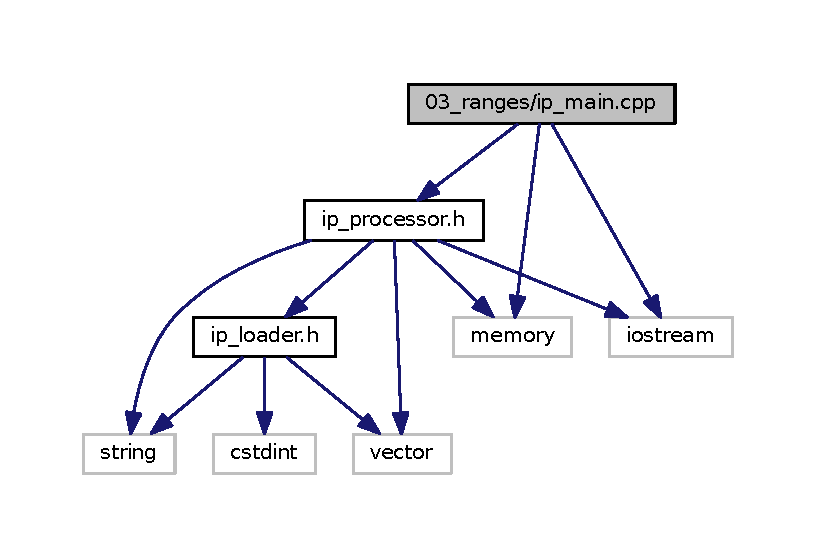
\includegraphics[width=350pt]{03__ranges_2ip__main_8cpp__incl}
\end{center}
\end{figure}
\subsection*{Functions}
\begin{DoxyCompactItemize}
\item 
int \hyperlink{03__ranges_2ip__main_8cpp_a0ddf1224851353fc92bfbff6f499fa97}{main} (int argc, char $\ast$argv\mbox{[}$\,$\mbox{]})
\end{DoxyCompactItemize}


\subsection{Function Documentation}
\index{03\+\_\+ranges/ip\+\_\+main.\+cpp@{03\+\_\+ranges/ip\+\_\+main.\+cpp}!main@{main}}
\index{main@{main}!03\+\_\+ranges/ip\+\_\+main.\+cpp@{03\+\_\+ranges/ip\+\_\+main.\+cpp}}
\subsubsection[{\texorpdfstring{main(int argc, char $\ast$argv[])}{main(int argc, char *argv[])}}]{\setlength{\rightskip}{0pt plus 5cm}int main (
\begin{DoxyParamCaption}
\item[{int}]{argc, }
\item[{char $\ast$}]{argv\mbox{[}$\,$\mbox{]}}
\end{DoxyParamCaption}
)}\hypertarget{03__ranges_2ip__main_8cpp_a0ddf1224851353fc92bfbff6f499fa97}{}\label{03__ranges_2ip__main_8cpp_a0ddf1224851353fc92bfbff6f499fa97}

\hypertarget{02_2ip__processor_8cpp}{}\section{02/ip\+\_\+processor.cpp File Reference}
\label{02_2ip__processor_8cpp}\index{02/ip\+\_\+processor.\+cpp@{02/ip\+\_\+processor.\+cpp}}
{\ttfamily \#include \char`\"{}ip\+\_\+processor.\+h\char`\"{}}\\*
{\ttfamily \#include $<$iostream$>$}\\*
{\ttfamily \#include $<$algorithm$>$}\\*
{\ttfamily \#include $<$iterator$>$}\\*
{\ttfamily \#include $<$ostream$>$}\\*
Include dependency graph for ip\+\_\+processor.\+cpp\+:
\nopagebreak
\begin{figure}[H]
\begin{center}
\leavevmode
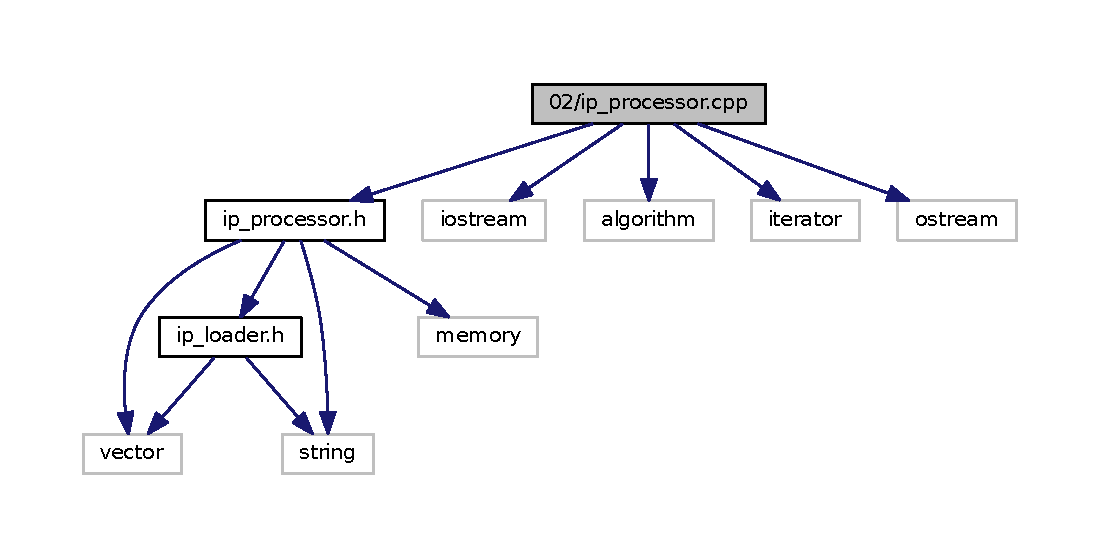
\includegraphics[width=350pt]{02_2ip__processor_8cpp__incl}
\end{center}
\end{figure}
\subsection*{Namespaces}
\begin{DoxyCompactItemize}
\item 
 \hyperlink{namespacestd}{std}
\end{DoxyCompactItemize}
\subsection*{Functions}
\begin{DoxyCompactItemize}
\item 
std\+::ostream \& \hyperlink{namespacestd_a985b65a9256bbd1a753db3025f101175}{std\+::operator$<$$<$} (std\+::ostream \&os, const std\+::vector$<$ std\+::string $>$ \&vs)
\item 
{\footnotesize template$<$typename Predicate $>$ }\\void \hyperlink{02_2ip__processor_8cpp_a6cb34919eb988bbeb21974a9623a7706}{print\+\_\+any\+\_\+condition} (const vector$<$ \hyperlink{02_2ip__loader_8h_ad6543533a9d8728e8ffbb208890f492e}{vec\+\_\+str} $>$ \&ippool, Predicate P1)
\end{DoxyCompactItemize}


\subsection{Function Documentation}
\index{02/ip\+\_\+processor.\+cpp@{02/ip\+\_\+processor.\+cpp}!print\+\_\+any\+\_\+condition@{print\+\_\+any\+\_\+condition}}
\index{print\+\_\+any\+\_\+condition@{print\+\_\+any\+\_\+condition}!02/ip\+\_\+processor.\+cpp@{02/ip\+\_\+processor.\+cpp}}
\subsubsection[{\texorpdfstring{print\+\_\+any\+\_\+condition(const vector$<$ vec\+\_\+str $>$ \&ippool, Predicate P1)}{print_any_condition(const vector< vec_str > &ippool, Predicate P1)}}]{\setlength{\rightskip}{0pt plus 5cm}template$<$typename Predicate $>$ void print\+\_\+any\+\_\+condition (
\begin{DoxyParamCaption}
\item[{const vector$<$ {\bf vec\+\_\+str} $>$ \&}]{ippool, }
\item[{Predicate}]{P1}
\end{DoxyParamCaption}
)}\hypertarget{02_2ip__processor_8cpp_a6cb34919eb988bbeb21974a9623a7706}{}\label{02_2ip__processor_8cpp_a6cb34919eb988bbeb21974a9623a7706}

\hypertarget{03__ranges_2ip__processor_8cpp}{}\section{03\+\_\+ranges/ip\+\_\+processor.cpp File Reference}
\label{03__ranges_2ip__processor_8cpp}\index{03\+\_\+ranges/ip\+\_\+processor.\+cpp@{03\+\_\+ranges/ip\+\_\+processor.\+cpp}}
{\ttfamily \#include \char`\"{}ip\+\_\+processor.\+h\char`\"{}}\\*
{\ttfamily \#include $<$iostream$>$}\\*
{\ttfamily \#include $<$algorithm$>$}\\*
{\ttfamily \#include $<$iterator$>$}\\*
{\ttfamily \#include $<$ostream$>$}\\*
{\ttfamily \#include $<$range/v3/all.\+hpp$>$}\\*
{\ttfamily \#include $<$range/v3/algorithm/sort.\+hpp$>$}\\*
Include dependency graph for ip\+\_\+processor.\+cpp\+:
\nopagebreak
\begin{figure}[H]
\begin{center}
\leavevmode
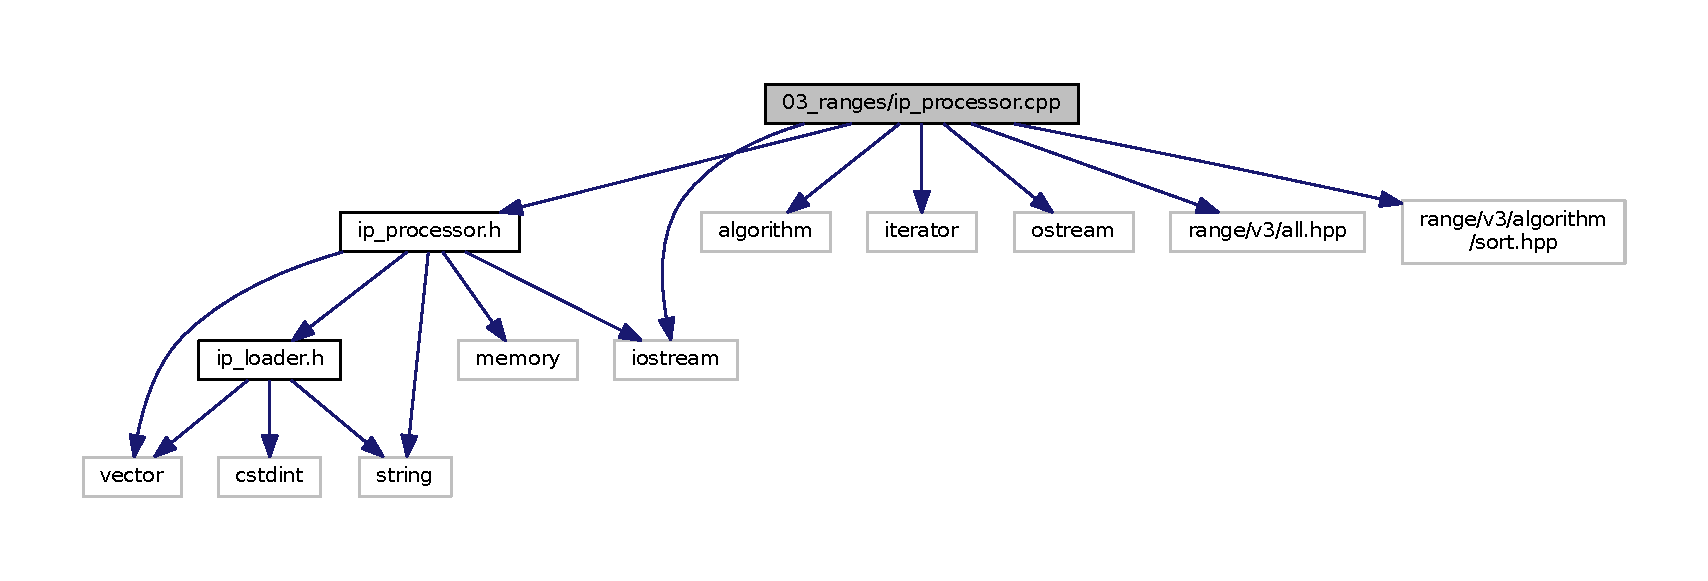
\includegraphics[width=350pt]{03__ranges_2ip__processor_8cpp__incl}
\end{center}
\end{figure}
\subsection*{Namespaces}
\begin{DoxyCompactItemize}
\item 
 \hyperlink{namespacestd}{std}
\end{DoxyCompactItemize}
\subsection*{Functions}
\begin{DoxyCompactItemize}
\item 
std\+::ostream \& \hyperlink{namespacestd_abb27abe27271b88570c789062cb2089a}{std\+::operator$<$$<$} (std\+::ostream \&os, const \hyperlink{03__ranges_2ip__loader_8h_adf9c1fa121650f19b895ecb6217615f2}{vec\+\_\+ui8} \&vs)
\item 
void \hyperlink{03__ranges_2ip__processor_8cpp_a79396c609a09a70fc948375f89e75a35}{print} (const vector$<$ \hyperlink{03__ranges_2ip__loader_8h_adf9c1fa121650f19b895ecb6217615f2}{vec\+\_\+ui8} $>$ \&ippool, std\+::ostream \&output)
\end{DoxyCompactItemize}


\subsection{Function Documentation}
\index{03\+\_\+ranges/ip\+\_\+processor.\+cpp@{03\+\_\+ranges/ip\+\_\+processor.\+cpp}!print@{print}}
\index{print@{print}!03\+\_\+ranges/ip\+\_\+processor.\+cpp@{03\+\_\+ranges/ip\+\_\+processor.\+cpp}}
\subsubsection[{\texorpdfstring{print(const vector$<$ vec\+\_\+ui8 $>$ \&ippool, std\+::ostream \&output)}{print(const vector< vec_ui8 > &ippool, std::ostream &output)}}]{\setlength{\rightskip}{0pt plus 5cm}void print (
\begin{DoxyParamCaption}
\item[{const vector$<$ {\bf vec\+\_\+ui8} $>$ \&}]{ippool, }
\item[{std\+::ostream \&}]{output}
\end{DoxyParamCaption}
)}\hypertarget{03__ranges_2ip__processor_8cpp_a79396c609a09a70fc948375f89e75a35}{}\label{03__ranges_2ip__processor_8cpp_a79396c609a09a70fc948375f89e75a35}

\hypertarget{02_2ip__processor_8h}{}\section{02/ip\+\_\+processor.h File Reference}
\label{02_2ip__processor_8h}\index{02/ip\+\_\+processor.\+h@{02/ip\+\_\+processor.\+h}}
{\ttfamily \#include \char`\"{}ip\+\_\+loader.\+h\char`\"{}}\\*
{\ttfamily \#include $<$memory$>$}\\*
{\ttfamily \#include $<$vector$>$}\\*
{\ttfamily \#include $<$string$>$}\\*
Include dependency graph for ip\+\_\+processor.\+h\+:
\nopagebreak
\begin{figure}[H]
\begin{center}
\leavevmode
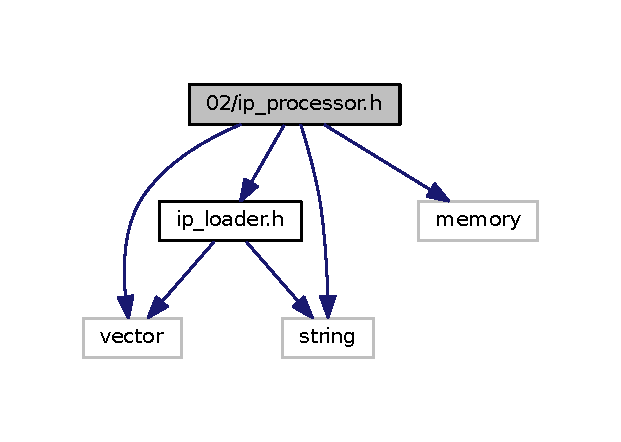
\includegraphics[width=298pt]{02_2ip__processor_8h__incl}
\end{center}
\end{figure}
This graph shows which files directly or indirectly include this file\+:
\nopagebreak
\begin{figure}[H]
\begin{center}
\leavevmode
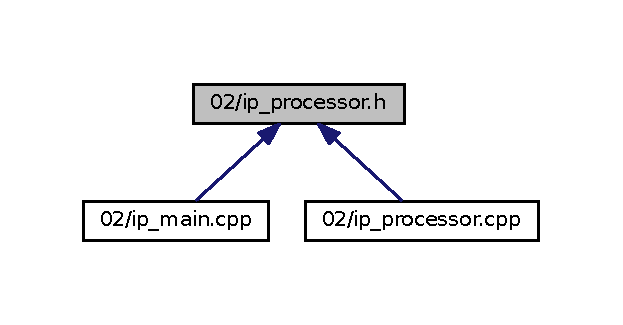
\includegraphics[width=299pt]{02_2ip__processor_8h__dep__incl}
\end{center}
\end{figure}
\subsection*{Classes}
\begin{DoxyCompactItemize}
\item 
class \hyperlink{classIpProcessor}{Ip\+Processor}
\end{DoxyCompactItemize}

\hypertarget{03__ranges_2ip__processor_8h}{}\section{03\+\_\+ranges/ip\+\_\+processor.h File Reference}
\label{03__ranges_2ip__processor_8h}\index{03\+\_\+ranges/ip\+\_\+processor.\+h@{03\+\_\+ranges/ip\+\_\+processor.\+h}}
{\ttfamily \#include \char`\"{}ip\+\_\+loader.\+h\char`\"{}}\\*
{\ttfamily \#include $<$memory$>$}\\*
{\ttfamily \#include $<$vector$>$}\\*
{\ttfamily \#include $<$string$>$}\\*
{\ttfamily \#include $<$iostream$>$}\\*
Include dependency graph for ip\+\_\+processor.\+h\+:
\nopagebreak
\begin{figure}[H]
\begin{center}
\leavevmode
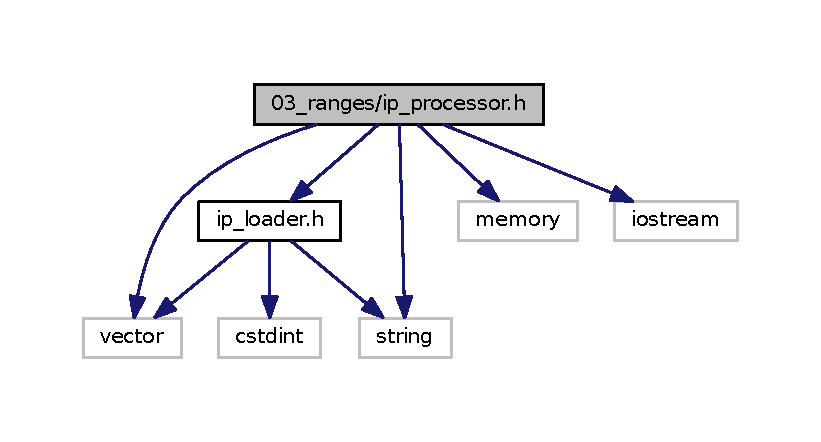
\includegraphics[width=350pt]{03__ranges_2ip__processor_8h__incl}
\end{center}
\end{figure}
This graph shows which files directly or indirectly include this file\+:
\nopagebreak
\begin{figure}[H]
\begin{center}
\leavevmode
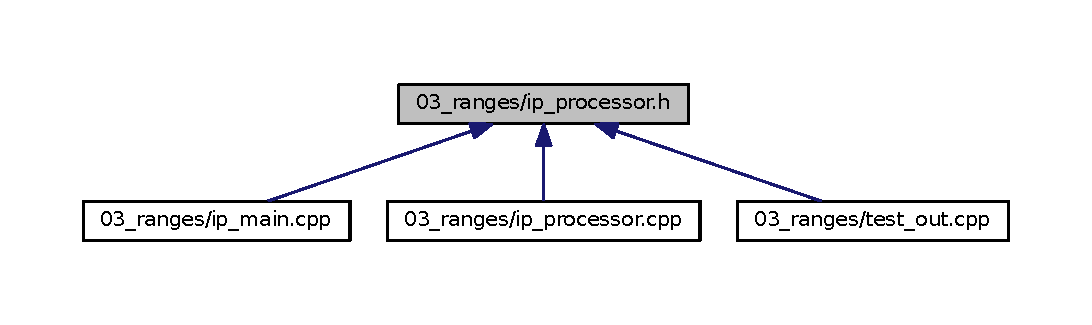
\includegraphics[width=350pt]{03__ranges_2ip__processor_8h__dep__incl}
\end{center}
\end{figure}
\subsection*{Classes}
\begin{DoxyCompactItemize}
\item 
class \hyperlink{classIpProcessor}{Ip\+Processor}
\end{DoxyCompactItemize}

\hypertarget{cstm__pair_8hpp}{}\section{02\+\_\+tuple/cstm\+\_\+pair.hpp File Reference}
\label{cstm__pair_8hpp}\index{02\+\_\+tuple/cstm\+\_\+pair.\+hpp@{02\+\_\+tuple/cstm\+\_\+pair.\+hpp}}
{\ttfamily \#include $<$algorithm$>$}\\*
{\ttfamily \#include $<$iostream$>$}\\*
{\ttfamily \#include $<$type\+\_\+traits$>$}\\*
Include dependency graph for cstm\+\_\+pair.\+hpp\+:
\nopagebreak
\begin{figure}[H]
\begin{center}
\leavevmode
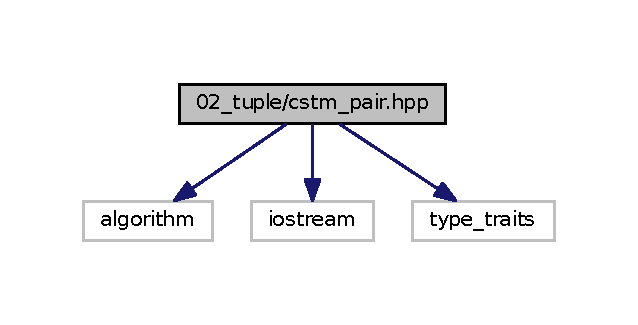
\includegraphics[width=306pt]{cstm__pair_8hpp__incl}
\end{center}
\end{figure}
This graph shows which files directly or indirectly include this file\+:
\nopagebreak
\begin{figure}[H]
\begin{center}
\leavevmode
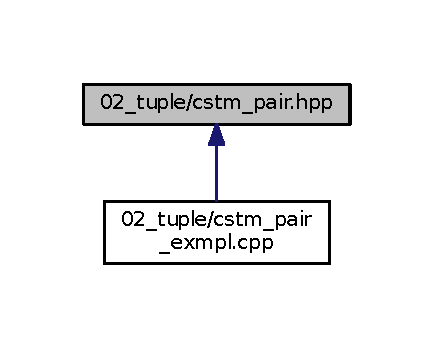
\includegraphics[width=208pt]{cstm__pair_8hpp__dep__incl}
\end{center}
\end{figure}
\subsection*{Classes}
\begin{DoxyCompactItemize}
\item 
class \hyperlink{classCustomPair}{Custom\+Pair$<$ T1, U2 $>$}
\item 
class \hyperlink{classCustomPair_3_01T1_01_6_00_01U2_01_6_01_4}{Custom\+Pair$<$ T1 \&, U2 \& $>$}
\end{DoxyCompactItemize}
\subsection*{Functions}
\begin{DoxyCompactItemize}
\item 
{\footnotesize template$<$typename T1 , typename U2 $>$ }\\std\+::ostream \& \hyperlink{cstm__pair_8hpp_a9e995341e5de1cd5b91e01ca94b519c4}{operator$<$$<$} (std\+::ostream \&os, const \hyperlink{classCustomPair}{Custom\+Pair}$<$ T1, U2 $>$ \&rhs\+\_\+pr)
\item 
{\footnotesize template$<$std\+::size\+\_\+t n, typename T1 , typename U2 $>$ }\\std\+::enable\+\_\+if$<$ n==0, T1 $>$\+::type \& \hyperlink{cstm__pair_8hpp_aefe0ca04fd4eca3c7e2e7629d28786eb}{get} (\hyperlink{classCustomPair}{Custom\+Pair}$<$ T1, U2 $>$ \&cstm\+\_\+pair)
\item 
{\footnotesize template$<$std\+::size\+\_\+t n, typename T1 , typename U2 $>$ }\\std\+::enable\+\_\+if$<$ n==1, U2 $>$\+::type \& \hyperlink{cstm__pair_8hpp_a97080eade9568466123a90d375487f2f}{get} (\hyperlink{classCustomPair}{Custom\+Pair}$<$ T1, U2 $>$ \&cstm\+\_\+pair)
\item 
{\footnotesize template$<$typename T1 , typename U2 $>$ }\\std\+::ostream \& \hyperlink{cstm__pair_8hpp_aa7814abf8ff90cf37d6a8c538977263e}{operator$<$$<$} (std\+::ostream \&os, const \hyperlink{classCustomPair}{Custom\+Pair}$<$ T1 \&, U2 \& $>$ \&rhs\+\_\+pr)
\item 
{\footnotesize template$<$typename T1 , typename U2 $>$ }\\\hyperlink{classCustomPair}{Custom\+Pair}$<$ T1 \&, U2 \& $>$ \hyperlink{cstm__pair_8hpp_a77134479457c9e9914f95c32359b4ac0}{custom\+\_\+tie} (T1 \&f, U2 \&s)
\item 
{\footnotesize template$<$typename T1 , typename U2 $>$ }\\\hyperlink{classCustomPair}{Custom\+Pair}$<$ T1, U2 $>$ \hyperlink{cstm__pair_8hpp_ac248ca822921e4d7885334626cb7e463}{make\+\_\+custom\+\_\+pair} (T1 f, U2 s)
\end{DoxyCompactItemize}


\subsection{Function Documentation}
\index{cstm\+\_\+pair.\+hpp@{cstm\+\_\+pair.\+hpp}!custom\+\_\+tie@{custom\+\_\+tie}}
\index{custom\+\_\+tie@{custom\+\_\+tie}!cstm\+\_\+pair.\+hpp@{cstm\+\_\+pair.\+hpp}}
\subsubsection[{\texorpdfstring{custom\+\_\+tie(\+T1 \&f, U2 \&s)}{custom_tie(T1 &f, U2 &s)}}]{\setlength{\rightskip}{0pt plus 5cm}template$<$typename T1 , typename U2 $>$ {\bf Custom\+Pair}$<$ T1 \&, U2 \& $>$ custom\+\_\+tie (
\begin{DoxyParamCaption}
\item[{T1 \&}]{f, }
\item[{U2 \&}]{s}
\end{DoxyParamCaption}
)}\hypertarget{cstm__pair_8hpp_a77134479457c9e9914f95c32359b4ac0}{}\label{cstm__pair_8hpp_a77134479457c9e9914f95c32359b4ac0}
\index{cstm\+\_\+pair.\+hpp@{cstm\+\_\+pair.\+hpp}!get@{get}}
\index{get@{get}!cstm\+\_\+pair.\+hpp@{cstm\+\_\+pair.\+hpp}}
\subsubsection[{\texorpdfstring{get(\+Custom\+Pair$<$ T1, U2 $>$ \&cstm\+\_\+pair)}{get(CustomPair< T1, U2 > &cstm_pair)}}]{\setlength{\rightskip}{0pt plus 5cm}template$<$std\+::size\+\_\+t n, typename T1 , typename U2 $>$ std\+::enable\+\_\+if$<$ n==0, T1 $>$\+::type \& get (
\begin{DoxyParamCaption}
\item[{{\bf Custom\+Pair}$<$ T1, U2 $>$ \&}]{cstm\+\_\+pair}
\end{DoxyParamCaption}
)}\hypertarget{cstm__pair_8hpp_aefe0ca04fd4eca3c7e2e7629d28786eb}{}\label{cstm__pair_8hpp_aefe0ca04fd4eca3c7e2e7629d28786eb}
\index{cstm\+\_\+pair.\+hpp@{cstm\+\_\+pair.\+hpp}!get@{get}}
\index{get@{get}!cstm\+\_\+pair.\+hpp@{cstm\+\_\+pair.\+hpp}}
\subsubsection[{\texorpdfstring{get(\+Custom\+Pair$<$ T1, U2 $>$ \&cstm\+\_\+pair)}{get(CustomPair< T1, U2 > &cstm_pair)}}]{\setlength{\rightskip}{0pt plus 5cm}template$<$std\+::size\+\_\+t n, typename T1 , typename U2 $>$ std\+::enable\+\_\+if$<$ n==1, U2 $>$\+::type \& get (
\begin{DoxyParamCaption}
\item[{{\bf Custom\+Pair}$<$ T1, U2 $>$ \&}]{cstm\+\_\+pair}
\end{DoxyParamCaption}
)}\hypertarget{cstm__pair_8hpp_a97080eade9568466123a90d375487f2f}{}\label{cstm__pair_8hpp_a97080eade9568466123a90d375487f2f}
\index{cstm\+\_\+pair.\+hpp@{cstm\+\_\+pair.\+hpp}!make\+\_\+custom\+\_\+pair@{make\+\_\+custom\+\_\+pair}}
\index{make\+\_\+custom\+\_\+pair@{make\+\_\+custom\+\_\+pair}!cstm\+\_\+pair.\+hpp@{cstm\+\_\+pair.\+hpp}}
\subsubsection[{\texorpdfstring{make\+\_\+custom\+\_\+pair(\+T1 f, U2 s)}{make_custom_pair(T1 f, U2 s)}}]{\setlength{\rightskip}{0pt plus 5cm}template$<$typename T1 , typename U2 $>$ {\bf Custom\+Pair}$<$T1, U2$>$ make\+\_\+custom\+\_\+pair (
\begin{DoxyParamCaption}
\item[{T1}]{f, }
\item[{U2}]{s}
\end{DoxyParamCaption}
)}\hypertarget{cstm__pair_8hpp_ac248ca822921e4d7885334626cb7e463}{}\label{cstm__pair_8hpp_ac248ca822921e4d7885334626cb7e463}
\index{cstm\+\_\+pair.\+hpp@{cstm\+\_\+pair.\+hpp}!operator$<$$<$@{operator$<$$<$}}
\index{operator$<$$<$@{operator$<$$<$}!cstm\+\_\+pair.\+hpp@{cstm\+\_\+pair.\+hpp}}
\subsubsection[{\texorpdfstring{operator$<$$<$(std\+::ostream \&os, const Custom\+Pair$<$ T1, U2 $>$ \&rhs\+\_\+pr)}{operator<<(std::ostream &os, const CustomPair< T1, U2 > &rhs_pr)}}]{\setlength{\rightskip}{0pt plus 5cm}template$<$typename T1 , typename U2 $>$ std\+::ostream \& operator$<$$<$ (
\begin{DoxyParamCaption}
\item[{std\+::ostream \&}]{os, }
\item[{const {\bf Custom\+Pair}$<$ T1, U2 $>$ \&}]{rhs\+\_\+pr}
\end{DoxyParamCaption}
)}\hypertarget{cstm__pair_8hpp_a9e995341e5de1cd5b91e01ca94b519c4}{}\label{cstm__pair_8hpp_a9e995341e5de1cd5b91e01ca94b519c4}
\index{cstm\+\_\+pair.\+hpp@{cstm\+\_\+pair.\+hpp}!operator$<$$<$@{operator$<$$<$}}
\index{operator$<$$<$@{operator$<$$<$}!cstm\+\_\+pair.\+hpp@{cstm\+\_\+pair.\+hpp}}
\subsubsection[{\texorpdfstring{operator$<$$<$(std\+::ostream \&os, const Custom\+Pair$<$ T1 \&, U2 \& $>$ \&rhs\+\_\+pr)}{operator<<(std::ostream &os, const CustomPair< T1 &, U2 & > &rhs_pr)}}]{\setlength{\rightskip}{0pt plus 5cm}template$<$typename T1 , typename U2 $>$ std\+::ostream \& operator$<$$<$ (
\begin{DoxyParamCaption}
\item[{std\+::ostream \&}]{os, }
\item[{const {\bf Custom\+Pair}$<$ T1 \&, U2 \& $>$ \&}]{rhs\+\_\+pr}
\end{DoxyParamCaption}
)}\hypertarget{cstm__pair_8hpp_aa7814abf8ff90cf37d6a8c538977263e}{}\label{cstm__pair_8hpp_aa7814abf8ff90cf37d6a8c538977263e}

\hypertarget{cstm__pair__2_8hpp}{}\section{02\+\_\+tuple/cstm\+\_\+pair\+\_\+2.hpp File Reference}
\label{cstm__pair__2_8hpp}\index{02\+\_\+tuple/cstm\+\_\+pair\+\_\+2.\+hpp@{02\+\_\+tuple/cstm\+\_\+pair\+\_\+2.\+hpp}}
{\ttfamily \#include $<$algorithm$>$}\\*
{\ttfamily \#include $<$iostream$>$}\\*
{\ttfamily \#include $<$type\+\_\+traits$>$}\\*
Include dependency graph for cstm\+\_\+pair\+\_\+2.\+hpp\+:
\nopagebreak
\begin{figure}[H]
\begin{center}
\leavevmode
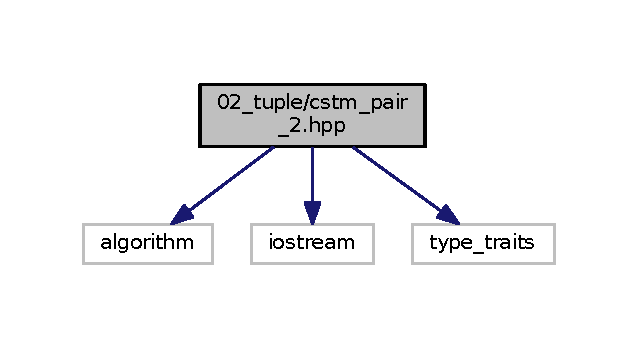
\includegraphics[width=306pt]{cstm__pair__2_8hpp__incl}
\end{center}
\end{figure}
This graph shows which files directly or indirectly include this file\+:
\nopagebreak
\begin{figure}[H]
\begin{center}
\leavevmode
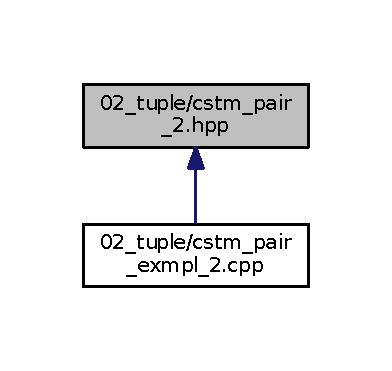
\includegraphics[width=188pt]{cstm__pair__2_8hpp__dep__incl}
\end{center}
\end{figure}
\subsection*{Classes}
\begin{DoxyCompactItemize}
\item 
class \hyperlink{classCustomPair2}{Custom\+Pair2$<$ T1, U2 $>$}
\end{DoxyCompactItemize}
\subsection*{Functions}
\begin{DoxyCompactItemize}
\item 
{\footnotesize template$<$typename T1 , typename U2 $>$ }\\std\+::ostream \& \hyperlink{cstm__pair__2_8hpp_a02d1c656174a47097d94b709c0b9a12c}{operator$<$$<$} (std\+::ostream \&os, const \hyperlink{classCustomPair2}{Custom\+Pair2}$<$ T1, U2 $>$ \&rhs\+\_\+pr)
\item 
{\footnotesize template$<$typename T1 , typename U2 $>$ }\\auto \hyperlink{cstm__pair__2_8hpp_afcf876dab5036d814a6ed52d0356ecab}{custom\+\_\+pair\+\_\+tie} (T1 \&\&f, U2 \&\&s)
\item 
{\footnotesize template$<$std\+::size\+\_\+t n, typename T1 , typename U2 $>$ }\\std\+::enable\+\_\+if$<$ n==0, T1 $>$\+::type \& \hyperlink{cstm__pair__2_8hpp_a4986bf935098b9486b29507d194f6dd5}{get} (\hyperlink{classCustomPair2}{Custom\+Pair2}$<$ T1, U2 $>$ \&cstm\+\_\+pair)
\item 
{\footnotesize template$<$std\+::size\+\_\+t n, typename T1 , typename U2 $>$ }\\std\+::enable\+\_\+if$<$ n==1, U2 $>$\+::type \& \hyperlink{cstm__pair__2_8hpp_ab9d7d7b66c9d6439474db97556119e8d}{get} (\hyperlink{classCustomPair2}{Custom\+Pair2}$<$ T1, U2 $>$ \&cstm\+\_\+pair)
\item 
{\footnotesize template$<$typename T1 , typename U2 $>$ }\\\hyperlink{classCustomPair2}{Custom\+Pair2}$<$ T1, U2 $>$ \hyperlink{cstm__pair__2_8hpp_ad5a0a11fc2b14a71c30b58814d0fc6e7}{make\+\_\+custom\+\_\+pair} (T1 f, U2 s)
\end{DoxyCompactItemize}


\subsection{Function Documentation}
\index{cstm\+\_\+pair\+\_\+2.\+hpp@{cstm\+\_\+pair\+\_\+2.\+hpp}!custom\+\_\+pair\+\_\+tie@{custom\+\_\+pair\+\_\+tie}}
\index{custom\+\_\+pair\+\_\+tie@{custom\+\_\+pair\+\_\+tie}!cstm\+\_\+pair\+\_\+2.\+hpp@{cstm\+\_\+pair\+\_\+2.\+hpp}}
\subsubsection[{\texorpdfstring{custom\+\_\+pair\+\_\+tie(\+T1 \&\&f, U2 \&\&s)}{custom_pair_tie(T1 &&f, U2 &&s)}}]{\setlength{\rightskip}{0pt plus 5cm}template$<$typename T1 , typename U2 $>$ auto custom\+\_\+pair\+\_\+tie (
\begin{DoxyParamCaption}
\item[{T1 \&\&}]{f, }
\item[{U2 \&\&}]{s}
\end{DoxyParamCaption}
)}\hypertarget{cstm__pair__2_8hpp_afcf876dab5036d814a6ed52d0356ecab}{}\label{cstm__pair__2_8hpp_afcf876dab5036d814a6ed52d0356ecab}
\index{cstm\+\_\+pair\+\_\+2.\+hpp@{cstm\+\_\+pair\+\_\+2.\+hpp}!get@{get}}
\index{get@{get}!cstm\+\_\+pair\+\_\+2.\+hpp@{cstm\+\_\+pair\+\_\+2.\+hpp}}
\subsubsection[{\texorpdfstring{get(\+Custom\+Pair2$<$ T1, U2 $>$ \&cstm\+\_\+pair)}{get(CustomPair2< T1, U2 > &cstm_pair)}}]{\setlength{\rightskip}{0pt plus 5cm}template$<$std\+::size\+\_\+t n, typename T1 , typename U2 $>$ std\+::enable\+\_\+if$<$ n==0, T1 $>$\+::type \& get (
\begin{DoxyParamCaption}
\item[{{\bf Custom\+Pair2}$<$ T1, U2 $>$ \&}]{cstm\+\_\+pair}
\end{DoxyParamCaption}
)}\hypertarget{cstm__pair__2_8hpp_a4986bf935098b9486b29507d194f6dd5}{}\label{cstm__pair__2_8hpp_a4986bf935098b9486b29507d194f6dd5}
\index{cstm\+\_\+pair\+\_\+2.\+hpp@{cstm\+\_\+pair\+\_\+2.\+hpp}!get@{get}}
\index{get@{get}!cstm\+\_\+pair\+\_\+2.\+hpp@{cstm\+\_\+pair\+\_\+2.\+hpp}}
\subsubsection[{\texorpdfstring{get(\+Custom\+Pair2$<$ T1, U2 $>$ \&cstm\+\_\+pair)}{get(CustomPair2< T1, U2 > &cstm_pair)}}]{\setlength{\rightskip}{0pt plus 5cm}template$<$std\+::size\+\_\+t n, typename T1 , typename U2 $>$ std\+::enable\+\_\+if$<$ n==1, U2 $>$\+::type \& get (
\begin{DoxyParamCaption}
\item[{{\bf Custom\+Pair2}$<$ T1, U2 $>$ \&}]{cstm\+\_\+pair}
\end{DoxyParamCaption}
)}\hypertarget{cstm__pair__2_8hpp_ab9d7d7b66c9d6439474db97556119e8d}{}\label{cstm__pair__2_8hpp_ab9d7d7b66c9d6439474db97556119e8d}
\index{cstm\+\_\+pair\+\_\+2.\+hpp@{cstm\+\_\+pair\+\_\+2.\+hpp}!make\+\_\+custom\+\_\+pair@{make\+\_\+custom\+\_\+pair}}
\index{make\+\_\+custom\+\_\+pair@{make\+\_\+custom\+\_\+pair}!cstm\+\_\+pair\+\_\+2.\+hpp@{cstm\+\_\+pair\+\_\+2.\+hpp}}
\subsubsection[{\texorpdfstring{make\+\_\+custom\+\_\+pair(\+T1 f, U2 s)}{make_custom_pair(T1 f, U2 s)}}]{\setlength{\rightskip}{0pt plus 5cm}template$<$typename T1 , typename U2 $>$ {\bf Custom\+Pair2}$<$T1, U2$>$ make\+\_\+custom\+\_\+pair (
\begin{DoxyParamCaption}
\item[{T1}]{f, }
\item[{U2}]{s}
\end{DoxyParamCaption}
)}\hypertarget{cstm__pair__2_8hpp_ad5a0a11fc2b14a71c30b58814d0fc6e7}{}\label{cstm__pair__2_8hpp_ad5a0a11fc2b14a71c30b58814d0fc6e7}
\index{cstm\+\_\+pair\+\_\+2.\+hpp@{cstm\+\_\+pair\+\_\+2.\+hpp}!operator$<$$<$@{operator$<$$<$}}
\index{operator$<$$<$@{operator$<$$<$}!cstm\+\_\+pair\+\_\+2.\+hpp@{cstm\+\_\+pair\+\_\+2.\+hpp}}
\subsubsection[{\texorpdfstring{operator$<$$<$(std\+::ostream \&os, const Custom\+Pair2$<$ T1, U2 $>$ \&rhs\+\_\+pr)}{operator<<(std::ostream &os, const CustomPair2< T1, U2 > &rhs_pr)}}]{\setlength{\rightskip}{0pt plus 5cm}template$<$typename T1 , typename U2 $>$ std\+::ostream \& operator$<$$<$ (
\begin{DoxyParamCaption}
\item[{std\+::ostream \&}]{os, }
\item[{const {\bf Custom\+Pair2}$<$ T1, U2 $>$ \&}]{rhs\+\_\+pr}
\end{DoxyParamCaption}
)}\hypertarget{cstm__pair__2_8hpp_a02d1c656174a47097d94b709c0b9a12c}{}\label{cstm__pair__2_8hpp_a02d1c656174a47097d94b709c0b9a12c}

\hypertarget{cstm__pair__exmpl_8cpp}{}\section{02\+\_\+tuple/cstm\+\_\+pair\+\_\+exmpl.cpp File Reference}
\label{cstm__pair__exmpl_8cpp}\index{02\+\_\+tuple/cstm\+\_\+pair\+\_\+exmpl.\+cpp@{02\+\_\+tuple/cstm\+\_\+pair\+\_\+exmpl.\+cpp}}
{\ttfamily \#include \char`\"{}cstm\+\_\+pair.\+hpp\char`\"{}}\\*
{\ttfamily \#include $<$iostream$>$}\\*
{\ttfamily \#include $<$string$>$}\\*
Include dependency graph for cstm\+\_\+pair\+\_\+exmpl.\+cpp\+:
\nopagebreak
\begin{figure}[H]
\begin{center}
\leavevmode
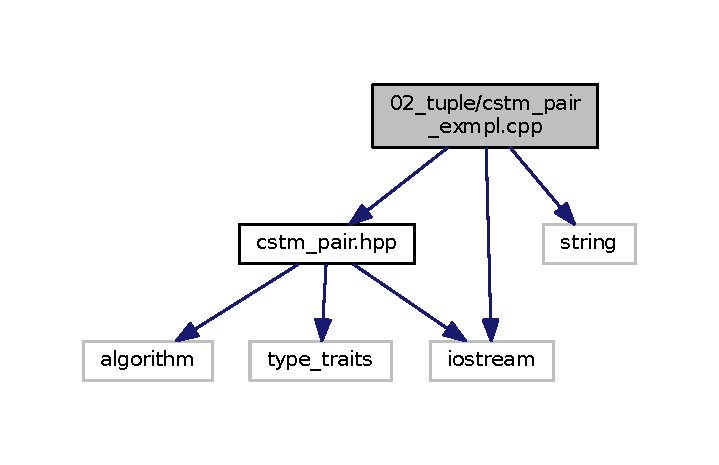
\includegraphics[width=345pt]{cstm__pair__exmpl_8cpp__incl}
\end{center}
\end{figure}
\subsection*{Functions}
\begin{DoxyCompactItemize}
\item 
auto \hyperlink{cstm__pair__exmpl_8cpp_ae67256938aa05b1d4bb49651db1d7acd}{get\+Person} ()
\item 
int \hyperlink{cstm__pair__exmpl_8cpp_a0ddf1224851353fc92bfbff6f499fa97}{main} (int argc, char $\ast$argv\mbox{[}$\,$\mbox{]})
\end{DoxyCompactItemize}


\subsection{Function Documentation}
\index{cstm\+\_\+pair\+\_\+exmpl.\+cpp@{cstm\+\_\+pair\+\_\+exmpl.\+cpp}!get\+Person@{get\+Person}}
\index{get\+Person@{get\+Person}!cstm\+\_\+pair\+\_\+exmpl.\+cpp@{cstm\+\_\+pair\+\_\+exmpl.\+cpp}}
\subsubsection[{\texorpdfstring{get\+Person()}{getPerson()}}]{\setlength{\rightskip}{0pt plus 5cm}auto get\+Person (
\begin{DoxyParamCaption}
{}
\end{DoxyParamCaption}
)}\hypertarget{cstm__pair__exmpl_8cpp_ae67256938aa05b1d4bb49651db1d7acd}{}\label{cstm__pair__exmpl_8cpp_ae67256938aa05b1d4bb49651db1d7acd}
\index{cstm\+\_\+pair\+\_\+exmpl.\+cpp@{cstm\+\_\+pair\+\_\+exmpl.\+cpp}!main@{main}}
\index{main@{main}!cstm\+\_\+pair\+\_\+exmpl.\+cpp@{cstm\+\_\+pair\+\_\+exmpl.\+cpp}}
\subsubsection[{\texorpdfstring{main(int argc, char $\ast$argv[])}{main(int argc, char *argv[])}}]{\setlength{\rightskip}{0pt plus 5cm}int main (
\begin{DoxyParamCaption}
\item[{int}]{argc, }
\item[{char $\ast$}]{argv\mbox{[}$\,$\mbox{]}}
\end{DoxyParamCaption}
)}\hypertarget{cstm__pair__exmpl_8cpp_a0ddf1224851353fc92bfbff6f499fa97}{}\label{cstm__pair__exmpl_8cpp_a0ddf1224851353fc92bfbff6f499fa97}

\hypertarget{cstm__pair__exmpl__2_8cpp}{}\section{02\+\_\+tuple/cstm\+\_\+pair\+\_\+exmpl\+\_\+2.cpp File Reference}
\label{cstm__pair__exmpl__2_8cpp}\index{02\+\_\+tuple/cstm\+\_\+pair\+\_\+exmpl\+\_\+2.\+cpp@{02\+\_\+tuple/cstm\+\_\+pair\+\_\+exmpl\+\_\+2.\+cpp}}
{\ttfamily \#include \char`\"{}cstm\+\_\+pair\+\_\+2.\+hpp\char`\"{}}\\*
{\ttfamily \#include $<$iostream$>$}\\*
{\ttfamily \#include $<$string$>$}\\*
Include dependency graph for cstm\+\_\+pair\+\_\+exmpl\+\_\+2.\+cpp\+:
\nopagebreak
\begin{figure}[H]
\begin{center}
\leavevmode
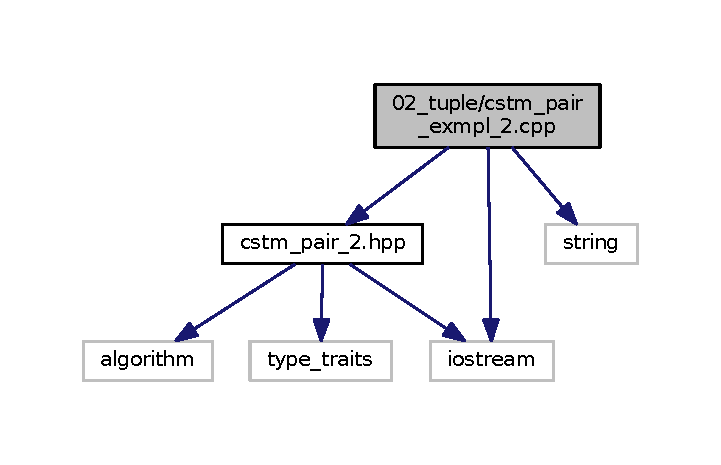
\includegraphics[width=346pt]{cstm__pair__exmpl__2_8cpp__incl}
\end{center}
\end{figure}
\subsection*{Functions}
\begin{DoxyCompactItemize}
\item 
auto \hyperlink{cstm__pair__exmpl__2_8cpp_ae67256938aa05b1d4bb49651db1d7acd}{get\+Person} ()
\item 
int \hyperlink{cstm__pair__exmpl__2_8cpp_a0ddf1224851353fc92bfbff6f499fa97}{main} (int argc, char $\ast$argv\mbox{[}$\,$\mbox{]})
\end{DoxyCompactItemize}


\subsection{Function Documentation}
\index{cstm\+\_\+pair\+\_\+exmpl\+\_\+2.\+cpp@{cstm\+\_\+pair\+\_\+exmpl\+\_\+2.\+cpp}!get\+Person@{get\+Person}}
\index{get\+Person@{get\+Person}!cstm\+\_\+pair\+\_\+exmpl\+\_\+2.\+cpp@{cstm\+\_\+pair\+\_\+exmpl\+\_\+2.\+cpp}}
\subsubsection[{\texorpdfstring{get\+Person()}{getPerson()}}]{\setlength{\rightskip}{0pt plus 5cm}auto get\+Person (
\begin{DoxyParamCaption}
{}
\end{DoxyParamCaption}
)}\hypertarget{cstm__pair__exmpl__2_8cpp_ae67256938aa05b1d4bb49651db1d7acd}{}\label{cstm__pair__exmpl__2_8cpp_ae67256938aa05b1d4bb49651db1d7acd}
\index{cstm\+\_\+pair\+\_\+exmpl\+\_\+2.\+cpp@{cstm\+\_\+pair\+\_\+exmpl\+\_\+2.\+cpp}!main@{main}}
\index{main@{main}!cstm\+\_\+pair\+\_\+exmpl\+\_\+2.\+cpp@{cstm\+\_\+pair\+\_\+exmpl\+\_\+2.\+cpp}}
\subsubsection[{\texorpdfstring{main(int argc, char $\ast$argv[])}{main(int argc, char *argv[])}}]{\setlength{\rightskip}{0pt plus 5cm}int main (
\begin{DoxyParamCaption}
\item[{int}]{argc, }
\item[{char $\ast$}]{argv\mbox{[}$\,$\mbox{]}}
\end{DoxyParamCaption}
)}\hypertarget{cstm__pair__exmpl__2_8cpp_a0ddf1224851353fc92bfbff6f499fa97}{}\label{cstm__pair__exmpl__2_8cpp_a0ddf1224851353fc92bfbff6f499fa97}

\hypertarget{cstm__tuple_8hpp}{}\section{02\+\_\+tuple/cstm\+\_\+tuple.hpp File Reference}
\label{cstm__tuple_8hpp}\index{02\+\_\+tuple/cstm\+\_\+tuple.\+hpp@{02\+\_\+tuple/cstm\+\_\+tuple.\+hpp}}
{\ttfamily \#include $<$iostream$>$}\\*
{\ttfamily \#include $<$string$>$}\\*
{\ttfamily \#include $<$cassert$>$}\\*
{\ttfamily \#include $<$cstdint$>$}\\*
{\ttfamily \#include $<$typeinfo$>$}\\*
{\ttfamily \#include $<$cstddef$>$}\\*
Include dependency graph for cstm\+\_\+tuple.\+hpp\+:
\nopagebreak
\begin{figure}[H]
\begin{center}
\leavevmode
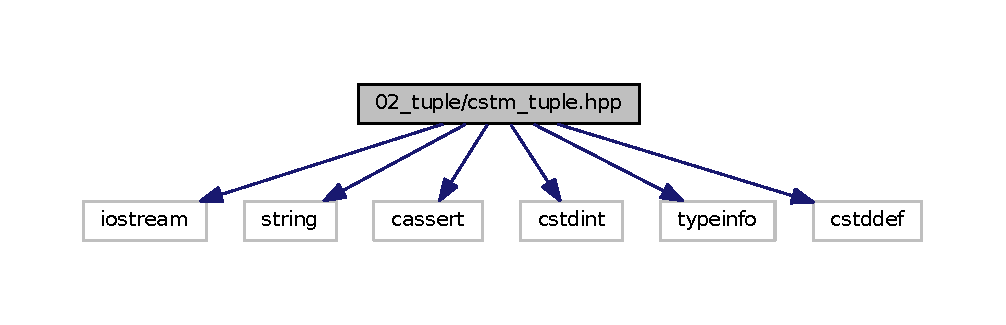
\includegraphics[width=350pt]{cstm__tuple_8hpp__incl}
\end{center}
\end{figure}
This graph shows which files directly or indirectly include this file\+:
\nopagebreak
\begin{figure}[H]
\begin{center}
\leavevmode
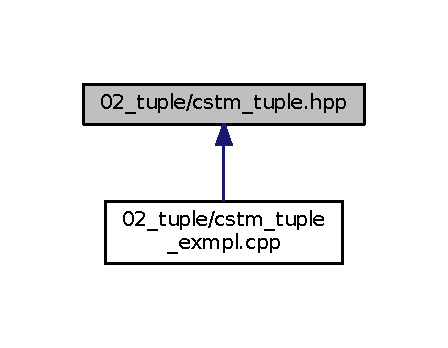
\includegraphics[width=215pt]{cstm__tuple_8hpp__dep__incl}
\end{center}
\end{figure}
\subsection*{Classes}
\begin{DoxyCompactItemize}
\item 
struct \hyperlink{structcustom__tuple}{custom\+\_\+tuple$<$ Types $>$}
\item 
struct \hyperlink{structcustom__tuple_3_01T_00_01Types_8_8_8_01_4}{custom\+\_\+tuple$<$ T, Types... $>$}
\item 
struct \hyperlink{structelem__type__holder}{elem\+\_\+type\+\_\+holder$<$ size\+\_\+t, typename $>$}
\item 
struct \hyperlink{structelem__type__holder_3_010_00_01custom__tuple_3_01T_00_01Ts_8_8_8_01_4_01_4}{elem\+\_\+type\+\_\+holder$<$ 0, custom\+\_\+tuple$<$ T, Ts... $>$ $>$}
\item 
struct \hyperlink{structelem__type__holder_3_01k_00_01custom__tuple_3_01T_00_01Ts_8_8_8_01_4_01_4}{elem\+\_\+type\+\_\+holder$<$ k, custom\+\_\+tuple$<$ T, Ts... $>$ $>$}
\end{DoxyCompactItemize}
\subsection*{Functions}
\begin{DoxyCompactItemize}
\item 
{\footnotesize template$<$size\+\_\+t k, typename... Types$>$ }\\std\+::enable\+\_\+if\+\_\+t$<$ k==0, typename \hyperlink{structelem__type__holder}{elem\+\_\+type\+\_\+holder}$<$ 0, \hyperlink{structcustom__tuple}{custom\+\_\+tuple}$<$ Types... $>$ $>$\+::type \& $>$ \hyperlink{cstm__tuple_8hpp_ace875a167aa434ff372f40dd99ac0694}{get} (\hyperlink{structcustom__tuple}{custom\+\_\+tuple}$<$ Types... $>$ \&ct)
\item 
{\footnotesize template$<$size\+\_\+t k, typename T , typename... Types$>$ }\\std\+::enable\+\_\+if\+\_\+t$<$ k!=0, typename \hyperlink{structelem__type__holder}{elem\+\_\+type\+\_\+holder}$<$ k, \hyperlink{structcustom__tuple}{custom\+\_\+tuple}$<$ T, Types... $>$ $>$\+::type \& $>$ \hyperlink{cstm__tuple_8hpp_aba451cbb702ef2407f373818725abcad}{get} (\hyperlink{structcustom__tuple}{custom\+\_\+tuple}$<$ T, Types... $>$ \&ct)
\item 
{\footnotesize template$<$typename... Types$>$ }\\auto \hyperlink{cstm__tuple_8hpp_aed4eda5a742f86f514dac3e022f8429d}{make\+\_\+custom\+\_\+tuple} (Types...\+args)
\item 
{\footnotesize template$<$typename... Types$>$ }\\auto \hyperlink{cstm__tuple_8hpp_a2afbfdeedd1bf8afc04f7849f4648f6c}{custom\+\_\+tie} (Types \&...args) noexcept
\end{DoxyCompactItemize}


\subsection{Function Documentation}
\index{cstm\+\_\+tuple.\+hpp@{cstm\+\_\+tuple.\+hpp}!custom\+\_\+tie@{custom\+\_\+tie}}
\index{custom\+\_\+tie@{custom\+\_\+tie}!cstm\+\_\+tuple.\+hpp@{cstm\+\_\+tuple.\+hpp}}
\subsubsection[{\texorpdfstring{custom\+\_\+tie(\+Types \&...\+args) noexcept}{custom_tie(Types &...args) noexcept}}]{\setlength{\rightskip}{0pt plus 5cm}template$<$typename... Types$>$ auto custom\+\_\+tie (
\begin{DoxyParamCaption}
\item[{Types \&...}]{args}
\end{DoxyParamCaption}
)\hspace{0.3cm}{\ttfamily [noexcept]}}\hypertarget{cstm__tuple_8hpp_a2afbfdeedd1bf8afc04f7849f4648f6c}{}\label{cstm__tuple_8hpp_a2afbfdeedd1bf8afc04f7849f4648f6c}
\index{cstm\+\_\+tuple.\+hpp@{cstm\+\_\+tuple.\+hpp}!get@{get}}
\index{get@{get}!cstm\+\_\+tuple.\+hpp@{cstm\+\_\+tuple.\+hpp}}
\subsubsection[{\texorpdfstring{get(custom\+\_\+tuple$<$ Types... $>$ \&ct)}{get(custom_tuple< Types... > &ct)}}]{\setlength{\rightskip}{0pt plus 5cm}template$<$size\+\_\+t k, typename... Types$>$ std\+::enable\+\_\+if\+\_\+t$<$k == 0, typename {\bf elem\+\_\+type\+\_\+holder}$<$0, {\bf custom\+\_\+tuple}$<$Types ... $>$ $>$\+::type\& $>$ get (
\begin{DoxyParamCaption}
\item[{{\bf custom\+\_\+tuple}$<$ Types... $>$ \&}]{ct}
\end{DoxyParamCaption}
)}\hypertarget{cstm__tuple_8hpp_ace875a167aa434ff372f40dd99ac0694}{}\label{cstm__tuple_8hpp_ace875a167aa434ff372f40dd99ac0694}
\index{cstm\+\_\+tuple.\+hpp@{cstm\+\_\+tuple.\+hpp}!get@{get}}
\index{get@{get}!cstm\+\_\+tuple.\+hpp@{cstm\+\_\+tuple.\+hpp}}
\subsubsection[{\texorpdfstring{get(custom\+\_\+tuple$<$ T, Types... $>$ \&ct)}{get(custom_tuple< T, Types... > &ct)}}]{\setlength{\rightskip}{0pt plus 5cm}template$<$size\+\_\+t k, typename T , typename... Types$>$ std\+::enable\+\_\+if\+\_\+t$<$k != 0, typename {\bf elem\+\_\+type\+\_\+holder}$<$k, {\bf custom\+\_\+tuple}$<$T, Types ... $>$ $>$\+::type \& $>$ get (
\begin{DoxyParamCaption}
\item[{{\bf custom\+\_\+tuple}$<$ T, Types... $>$ \&}]{ct}
\end{DoxyParamCaption}
)}\hypertarget{cstm__tuple_8hpp_aba451cbb702ef2407f373818725abcad}{}\label{cstm__tuple_8hpp_aba451cbb702ef2407f373818725abcad}
\index{cstm\+\_\+tuple.\+hpp@{cstm\+\_\+tuple.\+hpp}!make\+\_\+custom\+\_\+tuple@{make\+\_\+custom\+\_\+tuple}}
\index{make\+\_\+custom\+\_\+tuple@{make\+\_\+custom\+\_\+tuple}!cstm\+\_\+tuple.\+hpp@{cstm\+\_\+tuple.\+hpp}}
\subsubsection[{\texorpdfstring{make\+\_\+custom\+\_\+tuple(\+Types...\+args)}{make_custom_tuple(Types...args)}}]{\setlength{\rightskip}{0pt plus 5cm}template$<$typename... Types$>$ auto make\+\_\+custom\+\_\+tuple (
\begin{DoxyParamCaption}
\item[{Types...}]{args}
\end{DoxyParamCaption}
)}\hypertarget{cstm__tuple_8hpp_aed4eda5a742f86f514dac3e022f8429d}{}\label{cstm__tuple_8hpp_aed4eda5a742f86f514dac3e022f8429d}

\hypertarget{cstm__tuple__exmpl_8cpp}{}\section{02\+\_\+tuple/cstm\+\_\+tuple\+\_\+exmpl.cpp File Reference}
\label{cstm__tuple__exmpl_8cpp}\index{02\+\_\+tuple/cstm\+\_\+tuple\+\_\+exmpl.\+cpp@{02\+\_\+tuple/cstm\+\_\+tuple\+\_\+exmpl.\+cpp}}
{\ttfamily \#include \char`\"{}cstm\+\_\+tuple.\+hpp\char`\"{}}\\*
{\ttfamily \#include $<$string$>$}\\*
Include dependency graph for cstm\+\_\+tuple\+\_\+exmpl.\+cpp\+:
\nopagebreak
\begin{figure}[H]
\begin{center}
\leavevmode
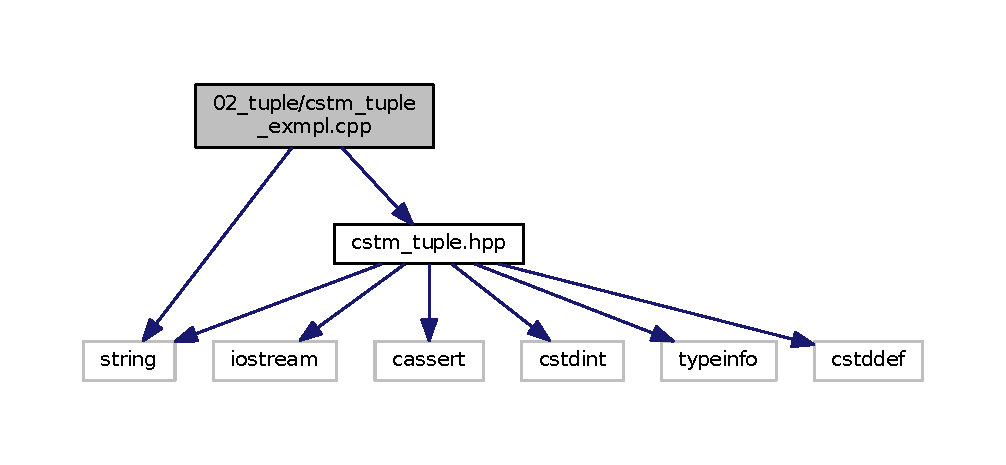
\includegraphics[width=350pt]{cstm__tuple__exmpl_8cpp__incl}
\end{center}
\end{figure}
\subsection*{Functions}
\begin{DoxyCompactItemize}
\item 
auto \hyperlink{cstm__tuple__exmpl_8cpp_ae67256938aa05b1d4bb49651db1d7acd}{get\+Person} ()
\item 
auto \hyperlink{cstm__tuple__exmpl_8cpp_a290da9ec9671d3f6d8be6f84c862678e}{get\+Person1} ()
\item 
int \hyperlink{cstm__tuple__exmpl_8cpp_a3c04138a5bfe5d72780bb7e82a18e627}{main} (int argc, char $\ast$$\ast$argv)
\end{DoxyCompactItemize}


\subsection{Function Documentation}
\index{cstm\+\_\+tuple\+\_\+exmpl.\+cpp@{cstm\+\_\+tuple\+\_\+exmpl.\+cpp}!get\+Person@{get\+Person}}
\index{get\+Person@{get\+Person}!cstm\+\_\+tuple\+\_\+exmpl.\+cpp@{cstm\+\_\+tuple\+\_\+exmpl.\+cpp}}
\subsubsection[{\texorpdfstring{get\+Person()}{getPerson()}}]{\setlength{\rightskip}{0pt plus 5cm}auto get\+Person (
\begin{DoxyParamCaption}
{}
\end{DoxyParamCaption}
)}\hypertarget{cstm__tuple__exmpl_8cpp_ae67256938aa05b1d4bb49651db1d7acd}{}\label{cstm__tuple__exmpl_8cpp_ae67256938aa05b1d4bb49651db1d7acd}
\index{cstm\+\_\+tuple\+\_\+exmpl.\+cpp@{cstm\+\_\+tuple\+\_\+exmpl.\+cpp}!get\+Person1@{get\+Person1}}
\index{get\+Person1@{get\+Person1}!cstm\+\_\+tuple\+\_\+exmpl.\+cpp@{cstm\+\_\+tuple\+\_\+exmpl.\+cpp}}
\subsubsection[{\texorpdfstring{get\+Person1()}{getPerson1()}}]{\setlength{\rightskip}{0pt plus 5cm}auto get\+Person1 (
\begin{DoxyParamCaption}
{}
\end{DoxyParamCaption}
)}\hypertarget{cstm__tuple__exmpl_8cpp_a290da9ec9671d3f6d8be6f84c862678e}{}\label{cstm__tuple__exmpl_8cpp_a290da9ec9671d3f6d8be6f84c862678e}
\index{cstm\+\_\+tuple\+\_\+exmpl.\+cpp@{cstm\+\_\+tuple\+\_\+exmpl.\+cpp}!main@{main}}
\index{main@{main}!cstm\+\_\+tuple\+\_\+exmpl.\+cpp@{cstm\+\_\+tuple\+\_\+exmpl.\+cpp}}
\subsubsection[{\texorpdfstring{main(int argc, char $\ast$$\ast$argv)}{main(int argc, char **argv)}}]{\setlength{\rightskip}{0pt plus 5cm}int main (
\begin{DoxyParamCaption}
\item[{int}]{argc, }
\item[{char $\ast$$\ast$}]{argv}
\end{DoxyParamCaption}
)}\hypertarget{cstm__tuple__exmpl_8cpp_a3c04138a5bfe5d72780bb7e82a18e627}{}\label{cstm__tuple__exmpl_8cpp_a3c04138a5bfe5d72780bb7e82a18e627}

\hypertarget{custom__container_8hpp}{}\section{03\+\_\+allocator/custom\+\_\+container.hpp File Reference}
\label{custom__container_8hpp}\index{03\+\_\+allocator/custom\+\_\+container.\+hpp@{03\+\_\+allocator/custom\+\_\+container.\+hpp}}
{\ttfamily \#include $<$memory$>$}\\*
{\ttfamily \#include $<$cstddef$>$}\\*
{\ttfamily \#include $<$iostream$>$}\\*
Include dependency graph for custom\+\_\+container.\+hpp\+:
\nopagebreak
\begin{figure}[H]
\begin{center}
\leavevmode
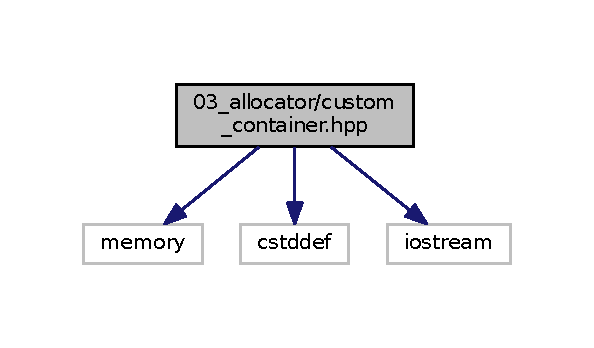
\includegraphics[width=285pt]{custom__container_8hpp__incl}
\end{center}
\end{figure}
This graph shows which files directly or indirectly include this file\+:
\nopagebreak
\begin{figure}[H]
\begin{center}
\leavevmode
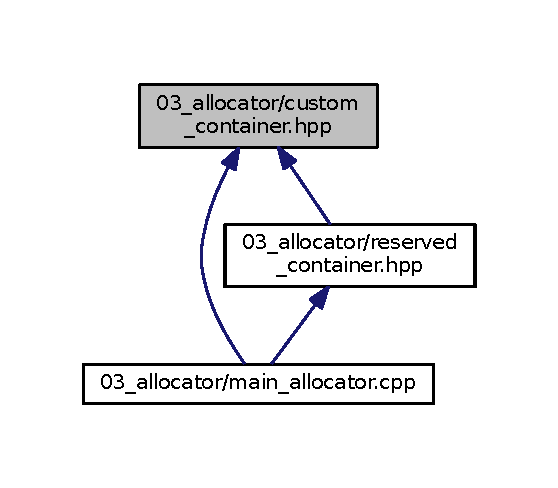
\includegraphics[width=268pt]{custom__container_8hpp__dep__incl}
\end{center}
\end{figure}
\subsection*{Classes}
\begin{DoxyCompactItemize}
\item 
class \hyperlink{classCustomContainer}{Custom\+Container$<$ T, allocator\+\_\+type $>$}
\end{DoxyCompactItemize}

\hypertarget{fixed__sz__allocator_8hpp}{}\section{03\+\_\+allocator/fixed\+\_\+sz\+\_\+allocator.hpp File Reference}
\label{fixed__sz__allocator_8hpp}\index{03\+\_\+allocator/fixed\+\_\+sz\+\_\+allocator.\+hpp@{03\+\_\+allocator/fixed\+\_\+sz\+\_\+allocator.\+hpp}}
{\ttfamily \#include $<$array$>$}\\*
{\ttfamily \#include $<$string$>$}\\*
{\ttfamily \#include $<$exception$>$}\\*
{\ttfamily \#include $<$iostream$>$}\\*
Include dependency graph for fixed\+\_\+sz\+\_\+allocator.\+hpp\+:
\nopagebreak
\begin{figure}[H]
\begin{center}
\leavevmode
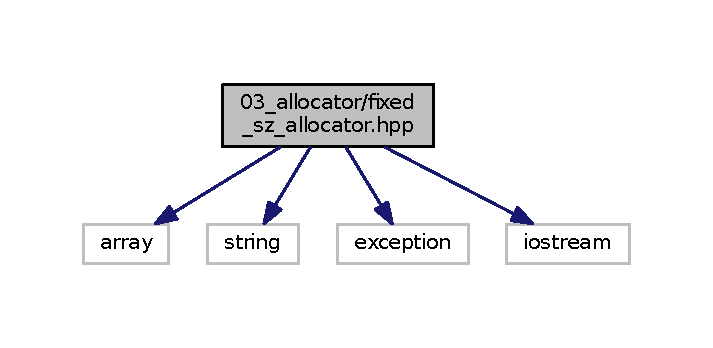
\includegraphics[width=342pt]{fixed__sz__allocator_8hpp__incl}
\end{center}
\end{figure}
This graph shows which files directly or indirectly include this file\+:
\nopagebreak
\begin{figure}[H]
\begin{center}
\leavevmode
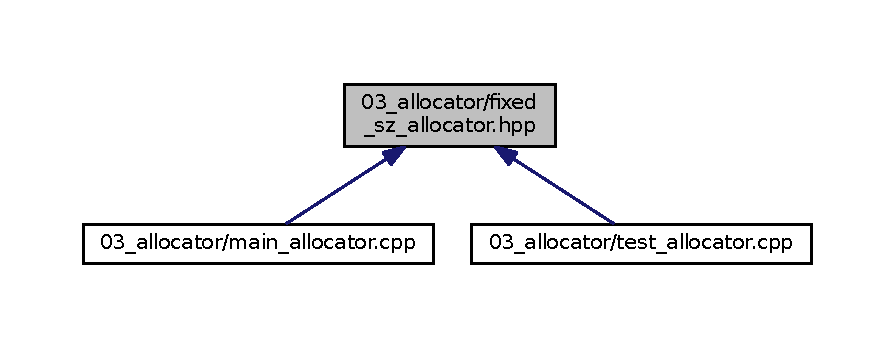
\includegraphics[width=350pt]{fixed__sz__allocator_8hpp__dep__incl}
\end{center}
\end{figure}
\subsection*{Classes}
\begin{DoxyCompactItemize}
\item 
class \hyperlink{classreserve__allocator}{reserve\+\_\+allocator$<$ T, n $>$}
\item 
struct \hyperlink{structreserve__allocator_1_1rebind}{reserve\+\_\+allocator$<$ T, n $>$\+::rebind$<$ U $>$}
\end{DoxyCompactItemize}

\hypertarget{flexible__allocator_8hpp}{}\section{03\+\_\+allocator/flexible\+\_\+allocator.hpp File Reference}
\label{flexible__allocator_8hpp}\index{03\+\_\+allocator/flexible\+\_\+allocator.\+hpp@{03\+\_\+allocator/flexible\+\_\+allocator.\+hpp}}
{\ttfamily \#include $<$cstddef$>$}\\*
{\ttfamily \#include $<$iostream$>$}\\*
{\ttfamily \#include $<$vector$>$}\\*
{\ttfamily \#include $<$memory$>$}\\*
{\ttfamily \#include $<$list$>$}\\*
Include dependency graph for flexible\+\_\+allocator.\+hpp\+:
\nopagebreak
\begin{figure}[H]
\begin{center}
\leavevmode
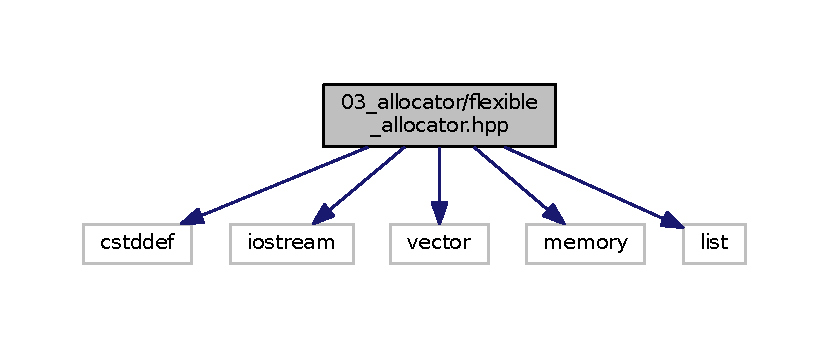
\includegraphics[width=350pt]{flexible__allocator_8hpp__incl}
\end{center}
\end{figure}
This graph shows which files directly or indirectly include this file\+:
\nopagebreak
\begin{figure}[H]
\begin{center}
\leavevmode
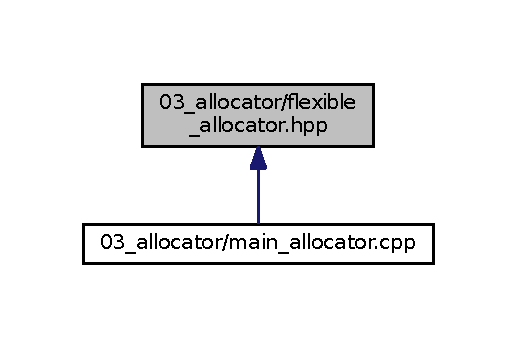
\includegraphics[width=248pt]{flexible__allocator_8hpp__dep__incl}
\end{center}
\end{figure}
\subsection*{Classes}
\begin{DoxyCompactItemize}
\item 
class \hyperlink{classcontigious__block}{contigious\+\_\+block$<$ T $>$}
\item 
class \hyperlink{classelementwise__block__allocator}{elementwise\+\_\+block\+\_\+allocator$<$ T $>$}
\end{DoxyCompactItemize}

\hypertarget{main__allocator_8cpp}{}\section{03\+\_\+allocator/main\+\_\+allocator.cpp File Reference}
\label{main__allocator_8cpp}\index{03\+\_\+allocator/main\+\_\+allocator.\+cpp@{03\+\_\+allocator/main\+\_\+allocator.\+cpp}}
{\ttfamily \#include \char`\"{}flexible\+\_\+allocator.\+hpp\char`\"{}}\\*
{\ttfamily \#include \char`\"{}fixed\+\_\+sz\+\_\+allocator.\+hpp\char`\"{}}\\*
{\ttfamily \#include \char`\"{}custom\+\_\+container.\+hpp\char`\"{}}\\*
{\ttfamily \#include \char`\"{}reserved\+\_\+container.\+hpp\char`\"{}}\\*
{\ttfamily \#include $<$iostream$>$}\\*
{\ttfamily \#include $<$map$>$}\\*
Include dependency graph for main\+\_\+allocator.\+cpp\+:
\nopagebreak
\begin{figure}[H]
\begin{center}
\leavevmode
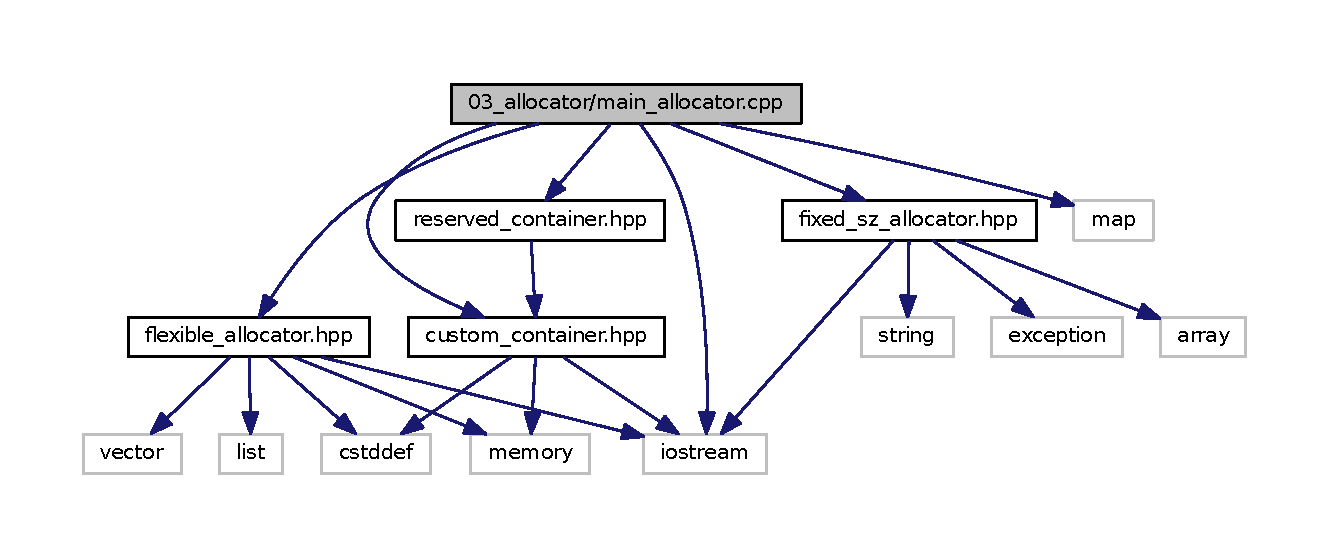
\includegraphics[width=350pt]{main__allocator_8cpp__incl}
\end{center}
\end{figure}
\subsection*{Functions}
\begin{DoxyCompactItemize}
\item 
int \hyperlink{main__allocator_8cpp_a0ddf1224851353fc92bfbff6f499fa97}{main} (int argc, char $\ast$argv\mbox{[}$\,$\mbox{]})
\end{DoxyCompactItemize}


\subsection{Function Documentation}
\index{main\+\_\+allocator.\+cpp@{main\+\_\+allocator.\+cpp}!main@{main}}
\index{main@{main}!main\+\_\+allocator.\+cpp@{main\+\_\+allocator.\+cpp}}
\subsubsection[{\texorpdfstring{main(int argc, char $\ast$argv[])}{main(int argc, char *argv[])}}]{\setlength{\rightskip}{0pt plus 5cm}int main (
\begin{DoxyParamCaption}
\item[{int}]{argc, }
\item[{char $\ast$}]{argv\mbox{[}$\,$\mbox{]}}
\end{DoxyParamCaption}
)}\hypertarget{main__allocator_8cpp_a0ddf1224851353fc92bfbff6f499fa97}{}\label{main__allocator_8cpp_a0ddf1224851353fc92bfbff6f499fa97}

\hypertarget{reserved__container_8hpp}{}\section{03\+\_\+allocator/reserved\+\_\+container.hpp File Reference}
\label{reserved__container_8hpp}\index{03\+\_\+allocator/reserved\+\_\+container.\+hpp@{03\+\_\+allocator/reserved\+\_\+container.\+hpp}}
{\ttfamily \#include \char`\"{}custom\+\_\+container.\+hpp\char`\"{}}\\*
Include dependency graph for reserved\+\_\+container.\+hpp\+:
\nopagebreak
\begin{figure}[H]
\begin{center}
\leavevmode
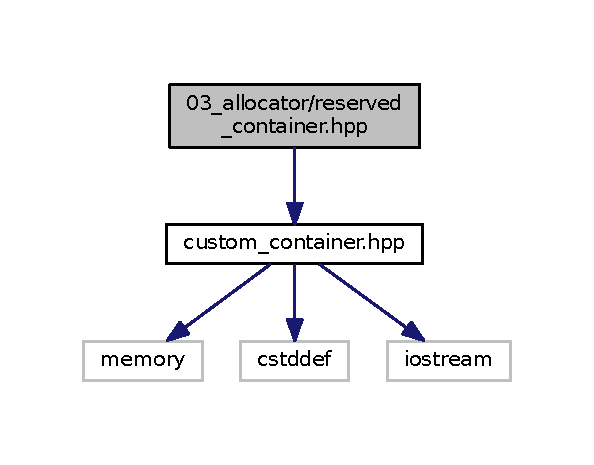
\includegraphics[width=285pt]{reserved__container_8hpp__incl}
\end{center}
\end{figure}
This graph shows which files directly or indirectly include this file\+:
\nopagebreak
\begin{figure}[H]
\begin{center}
\leavevmode
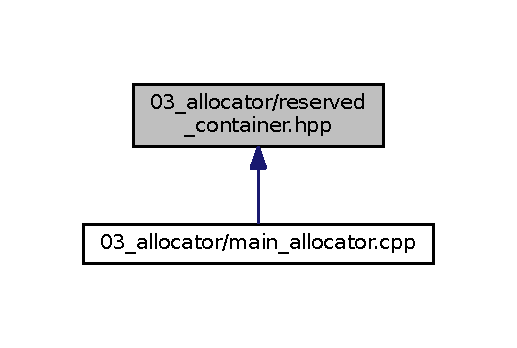
\includegraphics[width=248pt]{reserved__container_8hpp__dep__incl}
\end{center}
\end{figure}
\subsection*{Classes}
\begin{DoxyCompactItemize}
\item 
class \hyperlink{classCustomContainer_3_01T_00_01reserve__allocator_3_01T_00_01n_01_4_01_4}{Custom\+Container$<$ T, reserve\+\_\+allocator$<$ T, n $>$ $>$}
\end{DoxyCompactItemize}
\subsection*{Typedefs}
\begin{DoxyCompactItemize}
\item 
{\footnotesize template$<$typename T , size\+\_\+t n$>$ }\\using \hyperlink{reserved__container_8hpp_a645c90241dfa63f57e4e174b957f076a}{Reserved\+Container} = \hyperlink{classCustomContainer}{Custom\+Container}$<$ T, \hyperlink{classreserve__allocator}{reserve\+\_\+allocator}$<$ T, n $>$$>$
\end{DoxyCompactItemize}


\subsection{Typedef Documentation}
\index{reserved\+\_\+container.\+hpp@{reserved\+\_\+container.\+hpp}!Reserved\+Container@{Reserved\+Container}}
\index{Reserved\+Container@{Reserved\+Container}!reserved\+\_\+container.\+hpp@{reserved\+\_\+container.\+hpp}}
\subsubsection[{\texorpdfstring{Reserved\+Container}{ReservedContainer}}]{\setlength{\rightskip}{0pt plus 5cm}template$<$typename T , size\+\_\+t n$>$ using {\bf Reserved\+Container} =  {\bf Custom\+Container}$<$T, {\bf reserve\+\_\+allocator}$<$T, n$>$$>$}\hypertarget{reserved__container_8hpp_a645c90241dfa63f57e4e174b957f076a}{}\label{reserved__container_8hpp_a645c90241dfa63f57e4e174b957f076a}

\hypertarget{test__allocator_8cpp}{}\section{03\+\_\+allocator/test\+\_\+allocator.cpp File Reference}
\label{test__allocator_8cpp}\index{03\+\_\+allocator/test\+\_\+allocator.\+cpp@{03\+\_\+allocator/test\+\_\+allocator.\+cpp}}
{\ttfamily \#include \char`\"{}fixed\+\_\+sz\+\_\+allocator.\+hpp\char`\"{}}\\*
{\ttfamily \#include $<$gtest/gtest.\+h$>$}\\*
{\ttfamily \#include $<$iostream$>$}\\*
Include dependency graph for test\+\_\+allocator.\+cpp\+:
\nopagebreak
\begin{figure}[H]
\begin{center}
\leavevmode
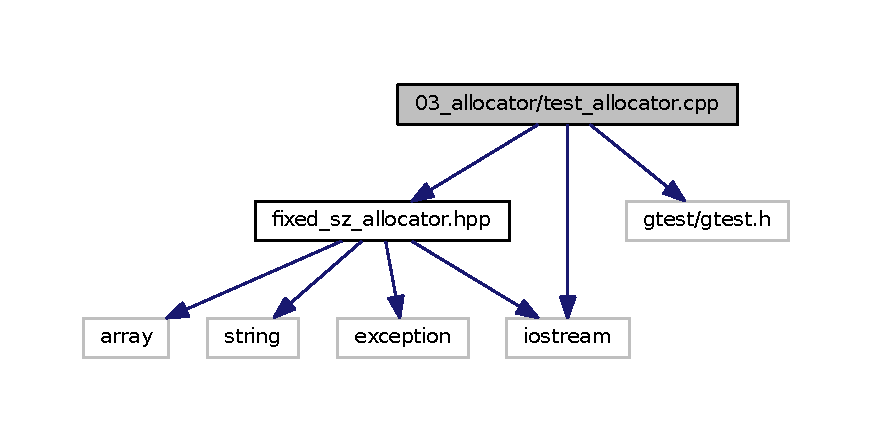
\includegraphics[width=350pt]{test__allocator_8cpp__incl}
\end{center}
\end{figure}
\subsection*{Functions}
\begin{DoxyCompactItemize}
\item 
\hyperlink{test__allocator_8cpp_a9a03f3ab02a05326d0e17811607fa4d4}{T\+E\+ST} (allocator, base\+\_\+operations)
\item 
\hyperlink{test__allocator_8cpp_a43054c06095011c4e988b8c2e744ff74}{T\+E\+ST} (allocator, insert\+\_\+operations)
\item 
\hyperlink{test__allocator_8cpp_aa3413cdc9a6ad9e8a89542a706e87e3d}{T\+E\+ST} (allocator, remove\+\_\+operations)
\item 
int \hyperlink{test__allocator_8cpp_a0ddf1224851353fc92bfbff6f499fa97}{main} (int argc, char $\ast$argv\mbox{[}$\,$\mbox{]})
\end{DoxyCompactItemize}


\subsection{Function Documentation}
\index{test\+\_\+allocator.\+cpp@{test\+\_\+allocator.\+cpp}!main@{main}}
\index{main@{main}!test\+\_\+allocator.\+cpp@{test\+\_\+allocator.\+cpp}}
\subsubsection[{\texorpdfstring{main(int argc, char $\ast$argv[])}{main(int argc, char *argv[])}}]{\setlength{\rightskip}{0pt plus 5cm}int main (
\begin{DoxyParamCaption}
\item[{int}]{argc, }
\item[{char $\ast$}]{argv\mbox{[}$\,$\mbox{]}}
\end{DoxyParamCaption}
)}\hypertarget{test__allocator_8cpp_a0ddf1224851353fc92bfbff6f499fa97}{}\label{test__allocator_8cpp_a0ddf1224851353fc92bfbff6f499fa97}
\index{test\+\_\+allocator.\+cpp@{test\+\_\+allocator.\+cpp}!T\+E\+ST@{T\+E\+ST}}
\index{T\+E\+ST@{T\+E\+ST}!test\+\_\+allocator.\+cpp@{test\+\_\+allocator.\+cpp}}
\subsubsection[{\texorpdfstring{T\+E\+S\+T(allocator, base\+\_\+operations)}{TEST(allocator, base_operations)}}]{\setlength{\rightskip}{0pt plus 5cm}T\+E\+ST (
\begin{DoxyParamCaption}
\item[{allocator}]{, }
\item[{base\+\_\+operations}]{}
\end{DoxyParamCaption}
)}\hypertarget{test__allocator_8cpp_a9a03f3ab02a05326d0e17811607fa4d4}{}\label{test__allocator_8cpp_a9a03f3ab02a05326d0e17811607fa4d4}
\index{test\+\_\+allocator.\+cpp@{test\+\_\+allocator.\+cpp}!T\+E\+ST@{T\+E\+ST}}
\index{T\+E\+ST@{T\+E\+ST}!test\+\_\+allocator.\+cpp@{test\+\_\+allocator.\+cpp}}
\subsubsection[{\texorpdfstring{T\+E\+S\+T(allocator, insert\+\_\+operations)}{TEST(allocator, insert_operations)}}]{\setlength{\rightskip}{0pt plus 5cm}T\+E\+ST (
\begin{DoxyParamCaption}
\item[{allocator}]{, }
\item[{insert\+\_\+operations}]{}
\end{DoxyParamCaption}
)}\hypertarget{test__allocator_8cpp_a43054c06095011c4e988b8c2e744ff74}{}\label{test__allocator_8cpp_a43054c06095011c4e988b8c2e744ff74}
\index{test\+\_\+allocator.\+cpp@{test\+\_\+allocator.\+cpp}!T\+E\+ST@{T\+E\+ST}}
\index{T\+E\+ST@{T\+E\+ST}!test\+\_\+allocator.\+cpp@{test\+\_\+allocator.\+cpp}}
\subsubsection[{\texorpdfstring{T\+E\+S\+T(allocator, remove\+\_\+operations)}{TEST(allocator, remove_operations)}}]{\setlength{\rightskip}{0pt plus 5cm}T\+E\+ST (
\begin{DoxyParamCaption}
\item[{allocator}]{, }
\item[{remove\+\_\+operations}]{}
\end{DoxyParamCaption}
)}\hypertarget{test__allocator_8cpp_aa3413cdc9a6ad9e8a89542a706e87e3d}{}\label{test__allocator_8cpp_aa3413cdc9a6ad9e8a89542a706e87e3d}

\hypertarget{test__out_8cpp}{}\section{03\+\_\+ranges/test\+\_\+out.cpp File Reference}
\label{test__out_8cpp}\index{03\+\_\+ranges/test\+\_\+out.\+cpp@{03\+\_\+ranges/test\+\_\+out.\+cpp}}
{\ttfamily \#include \char`\"{}ip\+\_\+processor.\+h\char`\"{}}\\*
{\ttfamily \#include $<$gtest/gtest.\+h$>$}\\*
{\ttfamily \#include $<$iostream$>$}\\*
{\ttfamily \#include $<$fstream$>$}\\*
{\ttfamily \#include $<$memory$>$}\\*
{\ttfamily \#include $<$cstdlib$>$}\\*
{\ttfamily \#include $<$cstdio$>$}\\*
Include dependency graph for test\+\_\+out.\+cpp\+:
\nopagebreak
\begin{figure}[H]
\begin{center}
\leavevmode
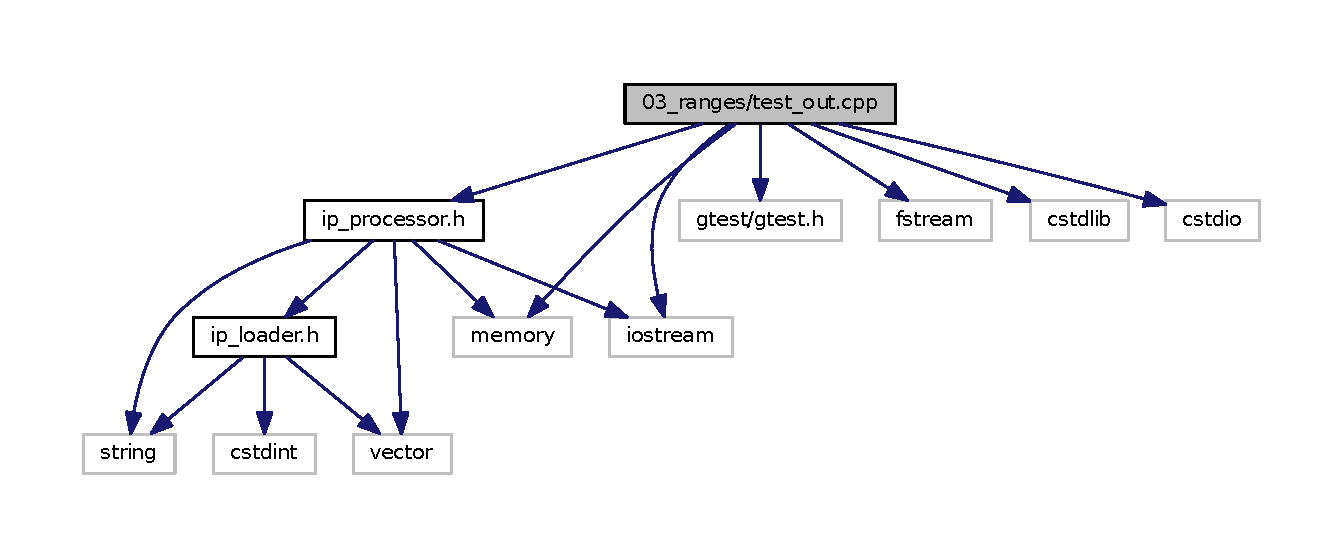
\includegraphics[width=350pt]{test__out_8cpp__incl}
\end{center}
\end{figure}
\subsection*{Functions}
\begin{DoxyCompactItemize}
\item 
\hyperlink{test__out_8cpp_a8ec24fc6035afdb0d266b9357c1cab9a}{T\+E\+ST} (test\+\_\+all\+\_\+results, ip)
\item 
int \hyperlink{test__out_8cpp_a0ddf1224851353fc92bfbff6f499fa97}{main} (int argc, char $\ast$argv\mbox{[}$\,$\mbox{]})
\end{DoxyCompactItemize}
\subsection*{Variables}
\begin{DoxyCompactItemize}
\item 
char $\ast$$\ast$ \hyperlink{test__out_8cpp_a05f58fe144fe2e6f1308c688cee7321c}{my\+\_\+argv}
\end{DoxyCompactItemize}


\subsection{Function Documentation}
\index{test\+\_\+out.\+cpp@{test\+\_\+out.\+cpp}!main@{main}}
\index{main@{main}!test\+\_\+out.\+cpp@{test\+\_\+out.\+cpp}}
\subsubsection[{\texorpdfstring{main(int argc, char $\ast$argv[])}{main(int argc, char *argv[])}}]{\setlength{\rightskip}{0pt plus 5cm}int main (
\begin{DoxyParamCaption}
\item[{int}]{argc, }
\item[{char $\ast$}]{argv\mbox{[}$\,$\mbox{]}}
\end{DoxyParamCaption}
)}\hypertarget{test__out_8cpp_a0ddf1224851353fc92bfbff6f499fa97}{}\label{test__out_8cpp_a0ddf1224851353fc92bfbff6f499fa97}
\index{test\+\_\+out.\+cpp@{test\+\_\+out.\+cpp}!T\+E\+ST@{T\+E\+ST}}
\index{T\+E\+ST@{T\+E\+ST}!test\+\_\+out.\+cpp@{test\+\_\+out.\+cpp}}
\subsubsection[{\texorpdfstring{T\+E\+S\+T(test\+\_\+all\+\_\+results, ip)}{TEST(test_all_results, ip)}}]{\setlength{\rightskip}{0pt plus 5cm}T\+E\+ST (
\begin{DoxyParamCaption}
\item[{test\+\_\+all\+\_\+results}]{, }
\item[{ip}]{}
\end{DoxyParamCaption}
)}\hypertarget{test__out_8cpp_a8ec24fc6035afdb0d266b9357c1cab9a}{}\label{test__out_8cpp_a8ec24fc6035afdb0d266b9357c1cab9a}


\subsection{Variable Documentation}
\index{test\+\_\+out.\+cpp@{test\+\_\+out.\+cpp}!my\+\_\+argv@{my\+\_\+argv}}
\index{my\+\_\+argv@{my\+\_\+argv}!test\+\_\+out.\+cpp@{test\+\_\+out.\+cpp}}
\subsubsection[{\texorpdfstring{my\+\_\+argv}{my_argv}}]{\setlength{\rightskip}{0pt plus 5cm}char$\ast$$\ast$ my\+\_\+argv}\hypertarget{test__out_8cpp_a05f58fe144fe2e6f1308c688cee7321c}{}\label{test__out_8cpp_a05f58fe144fe2e6f1308c688cee7321c}

\hypertarget{print__ip__04_8hpp}{}\section{04\+\_\+sfinae/print\+\_\+ip\+\_\+04.hpp File Reference}
\label{print__ip__04_8hpp}\index{04\+\_\+sfinae/print\+\_\+ip\+\_\+04.\+hpp@{04\+\_\+sfinae/print\+\_\+ip\+\_\+04.\+hpp}}
{\ttfamily \#include $<$type\+\_\+traits$>$}\\*
{\ttfamily \#include $<$iostream$>$}\\*
{\ttfamily \#include $<$string$>$}\\*
{\ttfamily \#include $<$vector$>$}\\*
{\ttfamily \#include $<$list$>$}\\*
{\ttfamily \#include $<$tuple$>$}\\*
{\ttfamily \#include $<$bitset$>$}\\*
{\ttfamily \#include $<$cstdint$>$}\\*
Include dependency graph for print\+\_\+ip\+\_\+04.\+hpp\+:
\nopagebreak
\begin{figure}[H]
\begin{center}
\leavevmode
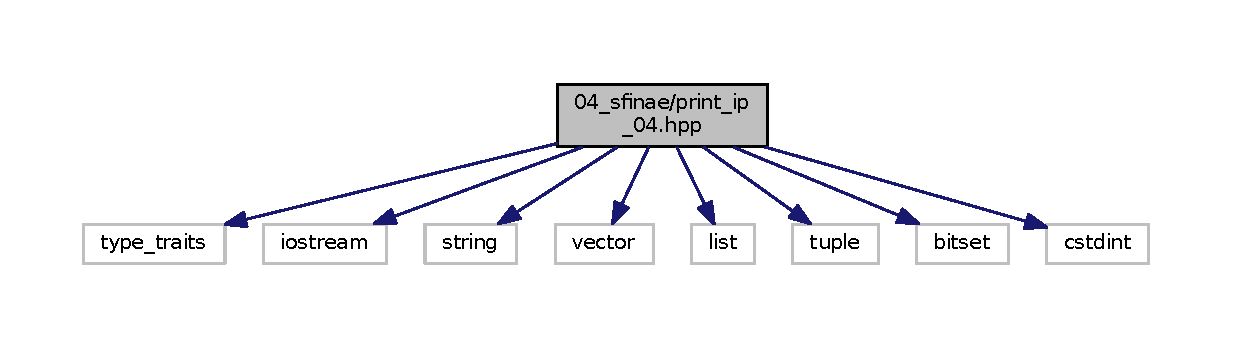
\includegraphics[width=350pt]{print__ip__04_8hpp__incl}
\end{center}
\end{figure}
This graph shows which files directly or indirectly include this file\+:
\nopagebreak
\begin{figure}[H]
\begin{center}
\leavevmode
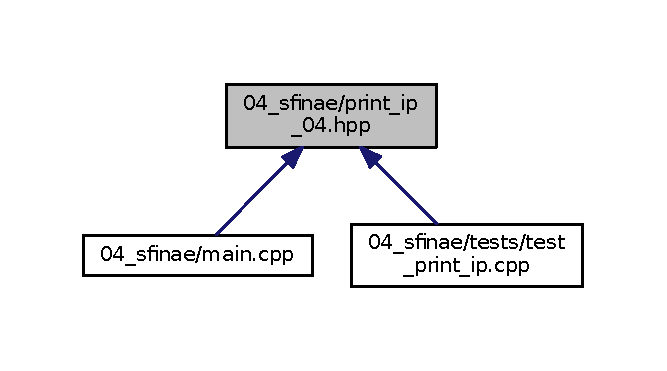
\includegraphics[width=320pt]{print__ip__04_8hpp__dep__incl}
\end{center}
\end{figure}
\subsection*{Classes}
\begin{DoxyCompactItemize}
\item 
struct \hyperlink{structis__std__string}{is\+\_\+std\+\_\+string$<$ T $>$}
\item 
struct \hyperlink{structis__std__string_3_01std_1_1string_01_4}{is\+\_\+std\+\_\+string$<$ std\+::string $>$}
\item 
struct \hyperlink{structis__std__container}{is\+\_\+std\+\_\+container$<$ T $>$}
\item 
struct \hyperlink{structis__std__container_3_01std_1_1vector_3_01T_01_4_01_4}{is\+\_\+std\+\_\+container$<$ std\+::vector$<$ T $>$ $>$}
\item 
struct \hyperlink{structis__std__container_3_01std_1_1list_3_01T_01_4_01_4}{is\+\_\+std\+\_\+container$<$ std\+::list$<$ T $>$ $>$}
\item 
struct \hyperlink{structare__types__same}{are\+\_\+types\+\_\+same$<$ Args $>$}
\item 
struct \hyperlink{structare__types__same_3_4}{are\+\_\+types\+\_\+same$<$$>$}
\item 
struct \hyperlink{structare__types__same_3_01T_01_4}{are\+\_\+types\+\_\+same$<$ T $>$}
\item 
struct \hyperlink{structare__types__same_3_01T_00_01U_00_01Args_8_8_8_01_4}{are\+\_\+types\+\_\+same$<$ T, U, Args... $>$}
\item 
struct \hyperlink{structis__uniform__args__tuple}{is\+\_\+uniform\+\_\+args\+\_\+tuple$<$ T $>$}
\item 
struct \hyperlink{structis__uniform__args__tuple_3_01std_1_1tuple_3_01Args_8_8_8_01_4_01_4}{is\+\_\+uniform\+\_\+args\+\_\+tuple$<$ std\+::tuple$<$ Args... $>$ $>$}
\item 
struct \hyperlink{structtupple__printer}{tupple\+\_\+printer$<$ Tuple, n $>$}
\item 
struct \hyperlink{structtupple__printer_3_01Tuple_00_011_01_4}{tupple\+\_\+printer$<$ Tuple, 1 $>$}
\end{DoxyCompactItemize}
\subsection*{Functions}
\begin{DoxyCompactItemize}
\item 
{\footnotesize template$<$typename T $>$ }\\void \hyperlink{print__ip__04_8hpp_a47fd58ec6c1ddc652352838383b380ff}{print\+\_\+item} (const std\+::string \&msg, const T item)
\item 
{\footnotesize template$<$typename T $>$ }\\std\+::enable\+\_\+if$<$ std\+::is\+\_\+integral$<$ T $>$\+::value, T $>$\+::type \hyperlink{print__ip__04_8hpp_a45be38d8c2df09aa103b97e5925fc7b2}{print\+\_\+ip} (T value)
\item 
{\footnotesize template$<$typename T $>$ }\\std\+::enable\+\_\+if$<$ \hyperlink{structis__std__string}{is\+\_\+std\+\_\+string}$<$ T $>$\+::value, T $>$\+::type \hyperlink{print__ip__04_8hpp_aa8515b28dac29decc4cf49c1884d8736}{print\+\_\+ip} (T value)
\item 
{\footnotesize template$<$typename T $>$ }\\std\+::enable\+\_\+if$<$ \hyperlink{structis__std__container}{is\+\_\+std\+\_\+container}$<$ T $>$\+::value, T $>$\+::type \hyperlink{print__ip__04_8hpp_ace42651894778994f10c54654ffd327e}{print\+\_\+ip} (T value)
\item 
{\footnotesize template$<$typename T $>$ }\\std\+::enable\+\_\+if$<$ \hyperlink{structis__uniform__args__tuple}{is\+\_\+uniform\+\_\+args\+\_\+tuple}$<$ T $>$\+::value, T $>$\+::type \hyperlink{print__ip__04_8hpp_a7f8cd2f2b3eedebf8d78cdc41fbe8b61}{print\+\_\+ip} (T value)
\end{DoxyCompactItemize}


\subsection{Function Documentation}
\index{print\+\_\+ip\+\_\+04.\+hpp@{print\+\_\+ip\+\_\+04.\+hpp}!print\+\_\+ip@{print\+\_\+ip}}
\index{print\+\_\+ip@{print\+\_\+ip}!print\+\_\+ip\+\_\+04.\+hpp@{print\+\_\+ip\+\_\+04.\+hpp}}
\subsubsection[{\texorpdfstring{print\+\_\+ip(\+T value)}{print_ip(T value)}}]{\setlength{\rightskip}{0pt plus 5cm}template$<$typename T $>$ std\+::enable\+\_\+if$<$std\+::is\+\_\+integral$<$T$>$\+::value, T$>$\+::type print\+\_\+ip (
\begin{DoxyParamCaption}
\item[{T}]{value}
\end{DoxyParamCaption}
)}\hypertarget{print__ip__04_8hpp_a45be38d8c2df09aa103b97e5925fc7b2}{}\label{print__ip__04_8hpp_a45be38d8c2df09aa103b97e5925fc7b2}
\index{print\+\_\+ip\+\_\+04.\+hpp@{print\+\_\+ip\+\_\+04.\+hpp}!print\+\_\+ip@{print\+\_\+ip}}
\index{print\+\_\+ip@{print\+\_\+ip}!print\+\_\+ip\+\_\+04.\+hpp@{print\+\_\+ip\+\_\+04.\+hpp}}
\subsubsection[{\texorpdfstring{print\+\_\+ip(\+T value)}{print_ip(T value)}}]{\setlength{\rightskip}{0pt plus 5cm}template$<$typename T $>$ std\+::enable\+\_\+if$<${\bf is\+\_\+std\+\_\+string}$<$T$>$\+::value, T$>$\+::type print\+\_\+ip (
\begin{DoxyParamCaption}
\item[{T}]{value}
\end{DoxyParamCaption}
)}\hypertarget{print__ip__04_8hpp_aa8515b28dac29decc4cf49c1884d8736}{}\label{print__ip__04_8hpp_aa8515b28dac29decc4cf49c1884d8736}
\index{print\+\_\+ip\+\_\+04.\+hpp@{print\+\_\+ip\+\_\+04.\+hpp}!print\+\_\+ip@{print\+\_\+ip}}
\index{print\+\_\+ip@{print\+\_\+ip}!print\+\_\+ip\+\_\+04.\+hpp@{print\+\_\+ip\+\_\+04.\+hpp}}
\subsubsection[{\texorpdfstring{print\+\_\+ip(\+T value)}{print_ip(T value)}}]{\setlength{\rightskip}{0pt plus 5cm}template$<$typename T $>$ std\+::enable\+\_\+if$<${\bf is\+\_\+std\+\_\+container}$<$T$>$\+::value, T$>$\+::type print\+\_\+ip (
\begin{DoxyParamCaption}
\item[{T}]{value}
\end{DoxyParamCaption}
)}\hypertarget{print__ip__04_8hpp_ace42651894778994f10c54654ffd327e}{}\label{print__ip__04_8hpp_ace42651894778994f10c54654ffd327e}
\index{print\+\_\+ip\+\_\+04.\+hpp@{print\+\_\+ip\+\_\+04.\+hpp}!print\+\_\+ip@{print\+\_\+ip}}
\index{print\+\_\+ip@{print\+\_\+ip}!print\+\_\+ip\+\_\+04.\+hpp@{print\+\_\+ip\+\_\+04.\+hpp}}
\subsubsection[{\texorpdfstring{print\+\_\+ip(\+T value)}{print_ip(T value)}}]{\setlength{\rightskip}{0pt plus 5cm}template$<$typename T $>$ std\+::enable\+\_\+if$<${\bf is\+\_\+uniform\+\_\+args\+\_\+tuple}$<$T$>$\+::value, T$>$\+::type print\+\_\+ip (
\begin{DoxyParamCaption}
\item[{T}]{value}
\end{DoxyParamCaption}
)}\hypertarget{print__ip__04_8hpp_a7f8cd2f2b3eedebf8d78cdc41fbe8b61}{}\label{print__ip__04_8hpp_a7f8cd2f2b3eedebf8d78cdc41fbe8b61}
\index{print\+\_\+ip\+\_\+04.\+hpp@{print\+\_\+ip\+\_\+04.\+hpp}!print\+\_\+item@{print\+\_\+item}}
\index{print\+\_\+item@{print\+\_\+item}!print\+\_\+ip\+\_\+04.\+hpp@{print\+\_\+ip\+\_\+04.\+hpp}}
\subsubsection[{\texorpdfstring{print\+\_\+item(const std\+::string \&msg, const T item)}{print_item(const std::string &msg, const T item)}}]{\setlength{\rightskip}{0pt plus 5cm}template$<$typename T $>$ void print\+\_\+item (
\begin{DoxyParamCaption}
\item[{const std\+::string \&}]{msg, }
\item[{const T}]{item}
\end{DoxyParamCaption}
)}\hypertarget{print__ip__04_8hpp_a47fd58ec6c1ddc652352838383b380ff}{}\label{print__ip__04_8hpp_a47fd58ec6c1ddc652352838383b380ff}

\hypertarget{test__print__ip_8cpp}{}\section{04\+\_\+sfinae/tests/test\+\_\+print\+\_\+ip.cpp File Reference}
\label{test__print__ip_8cpp}\index{04\+\_\+sfinae/tests/test\+\_\+print\+\_\+ip.\+cpp@{04\+\_\+sfinae/tests/test\+\_\+print\+\_\+ip.\+cpp}}
{\ttfamily \#include \char`\"{}../print\+\_\+ip\+\_\+04.\+hpp\char`\"{}}\\*
{\ttfamily \#include $<$gtest/gtest.\+h$>$}\\*
{\ttfamily \#include $<$iostream$>$}\\*
{\ttfamily \#include $<$memory$>$}\\*
Include dependency graph for test\+\_\+print\+\_\+ip.\+cpp\+:
\nopagebreak
\begin{figure}[H]
\begin{center}
\leavevmode
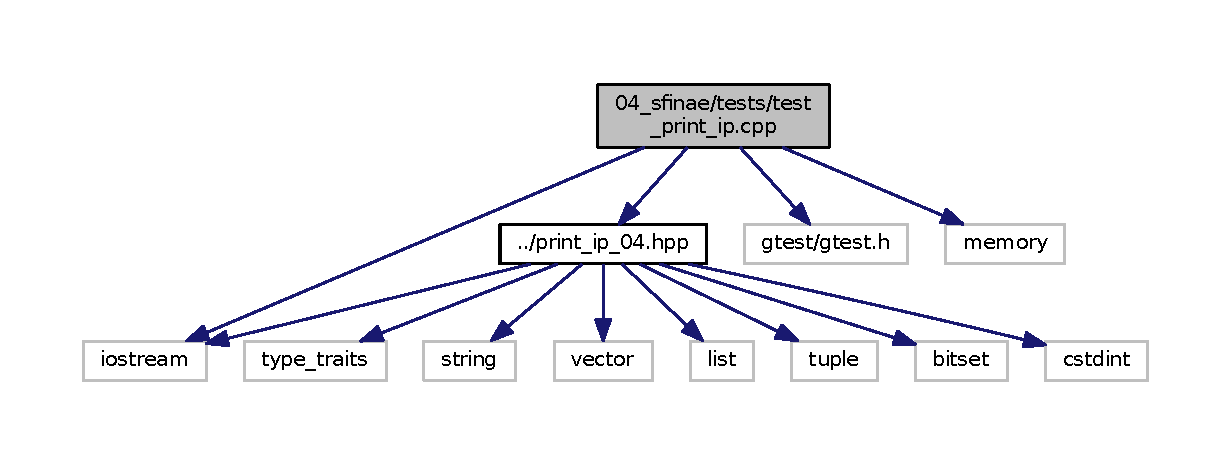
\includegraphics[width=350pt]{test__print__ip_8cpp__incl}
\end{center}
\end{figure}
\subsection*{Functions}
\begin{DoxyCompactItemize}
\item 
{\footnotesize template$<$typename T $>$ }\\void \hyperlink{test__print__ip_8cpp_a34d77df2d5074f8b2536f3c209574403}{test\+\_\+print\+\_\+ip} (T value, std\+::string ref\+\_\+result)
\item 
\hyperlink{test__print__ip_8cpp_a8ec24fc6035afdb0d266b9357c1cab9a}{T\+E\+ST} (test\+\_\+all\+\_\+results, ip)
\item 
int \hyperlink{test__print__ip_8cpp_a0ddf1224851353fc92bfbff6f499fa97}{main} (int argc, char $\ast$argv\mbox{[}$\,$\mbox{]})
\end{DoxyCompactItemize}


\subsection{Function Documentation}
\index{test\+\_\+print\+\_\+ip.\+cpp@{test\+\_\+print\+\_\+ip.\+cpp}!main@{main}}
\index{main@{main}!test\+\_\+print\+\_\+ip.\+cpp@{test\+\_\+print\+\_\+ip.\+cpp}}
\subsubsection[{\texorpdfstring{main(int argc, char $\ast$argv[])}{main(int argc, char *argv[])}}]{\setlength{\rightskip}{0pt plus 5cm}int main (
\begin{DoxyParamCaption}
\item[{int}]{argc, }
\item[{char $\ast$}]{argv\mbox{[}$\,$\mbox{]}}
\end{DoxyParamCaption}
)}\hypertarget{test__print__ip_8cpp_a0ddf1224851353fc92bfbff6f499fa97}{}\label{test__print__ip_8cpp_a0ddf1224851353fc92bfbff6f499fa97}
\index{test\+\_\+print\+\_\+ip.\+cpp@{test\+\_\+print\+\_\+ip.\+cpp}!T\+E\+ST@{T\+E\+ST}}
\index{T\+E\+ST@{T\+E\+ST}!test\+\_\+print\+\_\+ip.\+cpp@{test\+\_\+print\+\_\+ip.\+cpp}}
\subsubsection[{\texorpdfstring{T\+E\+S\+T(test\+\_\+all\+\_\+results, ip)}{TEST(test_all_results, ip)}}]{\setlength{\rightskip}{0pt plus 5cm}T\+E\+ST (
\begin{DoxyParamCaption}
\item[{test\+\_\+all\+\_\+results}]{, }
\item[{ip}]{}
\end{DoxyParamCaption}
)}\hypertarget{test__print__ip_8cpp_a8ec24fc6035afdb0d266b9357c1cab9a}{}\label{test__print__ip_8cpp_a8ec24fc6035afdb0d266b9357c1cab9a}
\index{test\+\_\+print\+\_\+ip.\+cpp@{test\+\_\+print\+\_\+ip.\+cpp}!test\+\_\+print\+\_\+ip@{test\+\_\+print\+\_\+ip}}
\index{test\+\_\+print\+\_\+ip@{test\+\_\+print\+\_\+ip}!test\+\_\+print\+\_\+ip.\+cpp@{test\+\_\+print\+\_\+ip.\+cpp}}
\subsubsection[{\texorpdfstring{test\+\_\+print\+\_\+ip(\+T value, std\+::string ref\+\_\+result)}{test_print_ip(T value, std::string ref_result)}}]{\setlength{\rightskip}{0pt plus 5cm}template$<$typename T $>$ void test\+\_\+print\+\_\+ip (
\begin{DoxyParamCaption}
\item[{T}]{value, }
\item[{std\+::string}]{ref\+\_\+result}
\end{DoxyParamCaption}
)}\hypertarget{test__print__ip_8cpp_a34d77df2d5074f8b2536f3c209574403}{}\label{test__print__ip_8cpp_a34d77df2d5074f8b2536f3c209574403}

\hypertarget{CMakeCCompilerId_8c}{}\section{C\+Make\+Files/3.12.4/\+Compiler\+Id\+C/\+C\+Make\+C\+Compiler\+Id.c File Reference}
\label{CMakeCCompilerId_8c}\index{C\+Make\+Files/3.\+12.\+4/\+Compiler\+Id\+C/\+C\+Make\+C\+Compiler\+Id.\+c@{C\+Make\+Files/3.\+12.\+4/\+Compiler\+Id\+C/\+C\+Make\+C\+Compiler\+Id.\+c}}
\subsection*{Macros}
\begin{DoxyCompactItemize}
\item 
\#define \hyperlink{CMakeCCompilerId_8c_a81dee0709ded976b2e0319239f72d174}{C\+O\+M\+P\+I\+L\+E\+R\+\_\+\+ID}~\char`\"{}\char`\"{}
\item 
\#define \hyperlink{CMakeCCompilerId_8c_a2ae9b72bb13abaabfcf2ee0ba7d3fa1d}{S\+T\+R\+I\+N\+G\+I\+F\+Y\+\_\+\+H\+E\+L\+P\+ER}(X)~\#X
\item 
\#define \hyperlink{CMakeCCompilerId_8c_a43e1cad902b6477bec893cb6430bd6c8}{S\+T\+R\+I\+N\+G\+I\+FY}(X)~\hyperlink{CMakeCXXCompilerId_8cpp_a2ae9b72bb13abaabfcf2ee0ba7d3fa1d}{S\+T\+R\+I\+N\+G\+I\+F\+Y\+\_\+\+H\+E\+L\+P\+ER}(X)
\item 
\#define \hyperlink{CMakeCCompilerId_8c_adbc5372f40838899018fadbc89bd588b}{P\+L\+A\+T\+F\+O\+R\+M\+\_\+\+ID}
\item 
\#define \hyperlink{CMakeCCompilerId_8c_aba35d0d200deaeb06aee95ca297acb28}{A\+R\+C\+H\+I\+T\+E\+C\+T\+U\+R\+E\+\_\+\+ID}
\item 
\#define \hyperlink{CMakeCCompilerId_8c_ad1280362da42492bbc11aa78cbf776ad}{D\+EC}(n)
\item 
\#define \hyperlink{CMakeCCompilerId_8c_a46d5d95daa1bef867bd0179594310ed5}{H\+EX}(n)
\item 
\#define \hyperlink{CMakeCCompilerId_8c_a07f8e5783674099cd7f5110e22a78cdb}{C\+\_\+\+D\+I\+A\+L\+E\+CT}
\end{DoxyCompactItemize}
\subsection*{Functions}
\begin{DoxyCompactItemize}
\item 
int \hyperlink{CMakeCCompilerId_8c_a0ddf1224851353fc92bfbff6f499fa97}{main} (int argc, char $\ast$argv\mbox{[}$\,$\mbox{]})
\end{DoxyCompactItemize}
\subsection*{Variables}
\begin{DoxyCompactItemize}
\item 
char const $\ast$ \hyperlink{CMakeCCompilerId_8c_a4b0efeb7a5d59313986b3a0390f050f6}{info\+\_\+compiler} = \char`\"{}I\+N\+FO\char`\"{} \char`\"{}\+:\char`\"{} \char`\"{}compiler\mbox{[}\char`\"{} C\+O\+M\+P\+I\+L\+E\+R\+\_\+\+ID \char`\"{}\mbox{]}\char`\"{}
\item 
char const $\ast$ \hyperlink{CMakeCCompilerId_8c_a2321403dee54ee23f0c2fa849c60f7d4}{info\+\_\+platform} = \char`\"{}I\+N\+FO\char`\"{} \char`\"{}\+:\char`\"{} \char`\"{}platform\mbox{[}\char`\"{} P\+L\+A\+T\+F\+O\+R\+M\+\_\+\+ID \char`\"{}\mbox{]}\char`\"{}
\item 
char const $\ast$ \hyperlink{CMakeCCompilerId_8c_a59647e99d304ed33b15cb284c27ed391}{info\+\_\+arch} = \char`\"{}I\+N\+FO\char`\"{} \char`\"{}\+:\char`\"{} \char`\"{}arch\mbox{[}\char`\"{} A\+R\+C\+H\+I\+T\+E\+C\+T\+U\+R\+E\+\_\+\+ID \char`\"{}\mbox{]}\char`\"{}
\item 
const char $\ast$ \hyperlink{CMakeCCompilerId_8c_a1ce162bad2fe6966ac8b33cc19e120b8}{info\+\_\+language\+\_\+dialect\+\_\+default}
\end{DoxyCompactItemize}


\subsection{Macro Definition Documentation}
\index{C\+Make\+C\+Compiler\+Id.\+c@{C\+Make\+C\+Compiler\+Id.\+c}!A\+R\+C\+H\+I\+T\+E\+C\+T\+U\+R\+E\+\_\+\+ID@{A\+R\+C\+H\+I\+T\+E\+C\+T\+U\+R\+E\+\_\+\+ID}}
\index{A\+R\+C\+H\+I\+T\+E\+C\+T\+U\+R\+E\+\_\+\+ID@{A\+R\+C\+H\+I\+T\+E\+C\+T\+U\+R\+E\+\_\+\+ID}!C\+Make\+C\+Compiler\+Id.\+c@{C\+Make\+C\+Compiler\+Id.\+c}}
\subsubsection[{\texorpdfstring{A\+R\+C\+H\+I\+T\+E\+C\+T\+U\+R\+E\+\_\+\+ID}{ARCHITECTURE_ID}}]{\setlength{\rightskip}{0pt plus 5cm}\#define A\+R\+C\+H\+I\+T\+E\+C\+T\+U\+R\+E\+\_\+\+ID}\hypertarget{CMakeCCompilerId_8c_aba35d0d200deaeb06aee95ca297acb28}{}\label{CMakeCCompilerId_8c_aba35d0d200deaeb06aee95ca297acb28}
\index{C\+Make\+C\+Compiler\+Id.\+c@{C\+Make\+C\+Compiler\+Id.\+c}!C\+\_\+\+D\+I\+A\+L\+E\+CT@{C\+\_\+\+D\+I\+A\+L\+E\+CT}}
\index{C\+\_\+\+D\+I\+A\+L\+E\+CT@{C\+\_\+\+D\+I\+A\+L\+E\+CT}!C\+Make\+C\+Compiler\+Id.\+c@{C\+Make\+C\+Compiler\+Id.\+c}}
\subsubsection[{\texorpdfstring{C\+\_\+\+D\+I\+A\+L\+E\+CT}{C_DIALECT}}]{\setlength{\rightskip}{0pt plus 5cm}\#define C\+\_\+\+D\+I\+A\+L\+E\+CT}\hypertarget{CMakeCCompilerId_8c_a07f8e5783674099cd7f5110e22a78cdb}{}\label{CMakeCCompilerId_8c_a07f8e5783674099cd7f5110e22a78cdb}
\index{C\+Make\+C\+Compiler\+Id.\+c@{C\+Make\+C\+Compiler\+Id.\+c}!C\+O\+M\+P\+I\+L\+E\+R\+\_\+\+ID@{C\+O\+M\+P\+I\+L\+E\+R\+\_\+\+ID}}
\index{C\+O\+M\+P\+I\+L\+E\+R\+\_\+\+ID@{C\+O\+M\+P\+I\+L\+E\+R\+\_\+\+ID}!C\+Make\+C\+Compiler\+Id.\+c@{C\+Make\+C\+Compiler\+Id.\+c}}
\subsubsection[{\texorpdfstring{C\+O\+M\+P\+I\+L\+E\+R\+\_\+\+ID}{COMPILER_ID}}]{\setlength{\rightskip}{0pt plus 5cm}\#define C\+O\+M\+P\+I\+L\+E\+R\+\_\+\+ID~\char`\"{}\char`\"{}}\hypertarget{CMakeCCompilerId_8c_a81dee0709ded976b2e0319239f72d174}{}\label{CMakeCCompilerId_8c_a81dee0709ded976b2e0319239f72d174}
\index{C\+Make\+C\+Compiler\+Id.\+c@{C\+Make\+C\+Compiler\+Id.\+c}!D\+EC@{D\+EC}}
\index{D\+EC@{D\+EC}!C\+Make\+C\+Compiler\+Id.\+c@{C\+Make\+C\+Compiler\+Id.\+c}}
\subsubsection[{\texorpdfstring{D\+EC}{DEC}}]{\setlength{\rightskip}{0pt plus 5cm}\#define D\+EC(
\begin{DoxyParamCaption}
\item[{}]{n}
\end{DoxyParamCaption}
)}\hypertarget{CMakeCCompilerId_8c_ad1280362da42492bbc11aa78cbf776ad}{}\label{CMakeCCompilerId_8c_ad1280362da42492bbc11aa78cbf776ad}
{\bfseries Value\+:}
\begin{DoxyCode}
(\textcolor{charliteral}{'0'} + (((n) / 10000000)%10)), \(\backslash\)
  (\textcolor{charliteral}{'0'} + (((n) / 1000000)%10)),  \(\backslash\)
  (\textcolor{charliteral}{'0'} + (((n) / 100000)%10)),   \(\backslash\)
  (\textcolor{charliteral}{'0'} + (((n) / 10000)%10)),    \(\backslash\)
  (\textcolor{charliteral}{'0'} + (((n) / 1000)%10)),     \(\backslash\)
  (\textcolor{charliteral}{'0'} + (((n) / 100)%10)),      \(\backslash\)
  (\textcolor{charliteral}{'0'} + (((n) / 10)%10)),       \(\backslash\)
  (\textcolor{charliteral}{'0'} +  ((n) % 10))
\end{DoxyCode}
\index{C\+Make\+C\+Compiler\+Id.\+c@{C\+Make\+C\+Compiler\+Id.\+c}!H\+EX@{H\+EX}}
\index{H\+EX@{H\+EX}!C\+Make\+C\+Compiler\+Id.\+c@{C\+Make\+C\+Compiler\+Id.\+c}}
\subsubsection[{\texorpdfstring{H\+EX}{HEX}}]{\setlength{\rightskip}{0pt plus 5cm}\#define H\+EX(
\begin{DoxyParamCaption}
\item[{}]{n}
\end{DoxyParamCaption}
)}\hypertarget{CMakeCCompilerId_8c_a46d5d95daa1bef867bd0179594310ed5}{}\label{CMakeCCompilerId_8c_a46d5d95daa1bef867bd0179594310ed5}
{\bfseries Value\+:}
\begin{DoxyCode}
(\textcolor{charliteral}{'0'} + ((n)>>28 & 0xF)), \(\backslash\)
  (\textcolor{charliteral}{'0'} + ((n)>>24 & 0xF)), \(\backslash\)
  (\textcolor{charliteral}{'0'} + ((n)>>20 & 0xF)), \(\backslash\)
  (\textcolor{charliteral}{'0'} + ((n)>>16 & 0xF)), \(\backslash\)
  (\textcolor{charliteral}{'0'} + ((n)>>12 & 0xF)), \(\backslash\)
  (\textcolor{charliteral}{'0'} + ((n)>>8  & 0xF)), \(\backslash\)
  (\textcolor{charliteral}{'0'} + ((n)>>4  & 0xF)), \(\backslash\)
  (\textcolor{charliteral}{'0'} + ((n)     & 0xF))
\end{DoxyCode}
\index{C\+Make\+C\+Compiler\+Id.\+c@{C\+Make\+C\+Compiler\+Id.\+c}!P\+L\+A\+T\+F\+O\+R\+M\+\_\+\+ID@{P\+L\+A\+T\+F\+O\+R\+M\+\_\+\+ID}}
\index{P\+L\+A\+T\+F\+O\+R\+M\+\_\+\+ID@{P\+L\+A\+T\+F\+O\+R\+M\+\_\+\+ID}!C\+Make\+C\+Compiler\+Id.\+c@{C\+Make\+C\+Compiler\+Id.\+c}}
\subsubsection[{\texorpdfstring{P\+L\+A\+T\+F\+O\+R\+M\+\_\+\+ID}{PLATFORM_ID}}]{\setlength{\rightskip}{0pt plus 5cm}\#define P\+L\+A\+T\+F\+O\+R\+M\+\_\+\+ID}\hypertarget{CMakeCCompilerId_8c_adbc5372f40838899018fadbc89bd588b}{}\label{CMakeCCompilerId_8c_adbc5372f40838899018fadbc89bd588b}
\index{C\+Make\+C\+Compiler\+Id.\+c@{C\+Make\+C\+Compiler\+Id.\+c}!S\+T\+R\+I\+N\+G\+I\+FY@{S\+T\+R\+I\+N\+G\+I\+FY}}
\index{S\+T\+R\+I\+N\+G\+I\+FY@{S\+T\+R\+I\+N\+G\+I\+FY}!C\+Make\+C\+Compiler\+Id.\+c@{C\+Make\+C\+Compiler\+Id.\+c}}
\subsubsection[{\texorpdfstring{S\+T\+R\+I\+N\+G\+I\+FY}{STRINGIFY}}]{\setlength{\rightskip}{0pt plus 5cm}\#define S\+T\+R\+I\+N\+G\+I\+FY(
\begin{DoxyParamCaption}
\item[{}]{X}
\end{DoxyParamCaption}
)~{\bf S\+T\+R\+I\+N\+G\+I\+F\+Y\+\_\+\+H\+E\+L\+P\+ER}(X)}\hypertarget{CMakeCCompilerId_8c_a43e1cad902b6477bec893cb6430bd6c8}{}\label{CMakeCCompilerId_8c_a43e1cad902b6477bec893cb6430bd6c8}
\index{C\+Make\+C\+Compiler\+Id.\+c@{C\+Make\+C\+Compiler\+Id.\+c}!S\+T\+R\+I\+N\+G\+I\+F\+Y\+\_\+\+H\+E\+L\+P\+ER@{S\+T\+R\+I\+N\+G\+I\+F\+Y\+\_\+\+H\+E\+L\+P\+ER}}
\index{S\+T\+R\+I\+N\+G\+I\+F\+Y\+\_\+\+H\+E\+L\+P\+ER@{S\+T\+R\+I\+N\+G\+I\+F\+Y\+\_\+\+H\+E\+L\+P\+ER}!C\+Make\+C\+Compiler\+Id.\+c@{C\+Make\+C\+Compiler\+Id.\+c}}
\subsubsection[{\texorpdfstring{S\+T\+R\+I\+N\+G\+I\+F\+Y\+\_\+\+H\+E\+L\+P\+ER}{STRINGIFY_HELPER}}]{\setlength{\rightskip}{0pt plus 5cm}\#define S\+T\+R\+I\+N\+G\+I\+F\+Y\+\_\+\+H\+E\+L\+P\+ER(
\begin{DoxyParamCaption}
\item[{}]{X}
\end{DoxyParamCaption}
)~\#X}\hypertarget{CMakeCCompilerId_8c_a2ae9b72bb13abaabfcf2ee0ba7d3fa1d}{}\label{CMakeCCompilerId_8c_a2ae9b72bb13abaabfcf2ee0ba7d3fa1d}


\subsection{Function Documentation}
\index{C\+Make\+C\+Compiler\+Id.\+c@{C\+Make\+C\+Compiler\+Id.\+c}!main@{main}}
\index{main@{main}!C\+Make\+C\+Compiler\+Id.\+c@{C\+Make\+C\+Compiler\+Id.\+c}}
\subsubsection[{\texorpdfstring{main(int argc, char $\ast$argv[])}{main(int argc, char *argv[])}}]{\setlength{\rightskip}{0pt plus 5cm}int main (
\begin{DoxyParamCaption}
\item[{int}]{argc, }
\item[{char $\ast$}]{argv\mbox{[}$\,$\mbox{]}}
\end{DoxyParamCaption}
)}\hypertarget{CMakeCCompilerId_8c_a0ddf1224851353fc92bfbff6f499fa97}{}\label{CMakeCCompilerId_8c_a0ddf1224851353fc92bfbff6f499fa97}


\subsection{Variable Documentation}
\index{C\+Make\+C\+Compiler\+Id.\+c@{C\+Make\+C\+Compiler\+Id.\+c}!info\+\_\+arch@{info\+\_\+arch}}
\index{info\+\_\+arch@{info\+\_\+arch}!C\+Make\+C\+Compiler\+Id.\+c@{C\+Make\+C\+Compiler\+Id.\+c}}
\subsubsection[{\texorpdfstring{info\+\_\+arch}{info_arch}}]{\setlength{\rightskip}{0pt plus 5cm}char const$\ast$ info\+\_\+arch = \char`\"{}I\+N\+FO\char`\"{} \char`\"{}\+:\char`\"{} \char`\"{}arch\mbox{[}\char`\"{} A\+R\+C\+H\+I\+T\+E\+C\+T\+U\+R\+E\+\_\+\+ID \char`\"{}\mbox{]}\char`\"{}}\hypertarget{CMakeCCompilerId_8c_a59647e99d304ed33b15cb284c27ed391}{}\label{CMakeCCompilerId_8c_a59647e99d304ed33b15cb284c27ed391}
\index{C\+Make\+C\+Compiler\+Id.\+c@{C\+Make\+C\+Compiler\+Id.\+c}!info\+\_\+compiler@{info\+\_\+compiler}}
\index{info\+\_\+compiler@{info\+\_\+compiler}!C\+Make\+C\+Compiler\+Id.\+c@{C\+Make\+C\+Compiler\+Id.\+c}}
\subsubsection[{\texorpdfstring{info\+\_\+compiler}{info_compiler}}]{\setlength{\rightskip}{0pt plus 5cm}char const$\ast$ info\+\_\+compiler = \char`\"{}I\+N\+FO\char`\"{} \char`\"{}\+:\char`\"{} \char`\"{}compiler\mbox{[}\char`\"{} C\+O\+M\+P\+I\+L\+E\+R\+\_\+\+ID \char`\"{}\mbox{]}\char`\"{}}\hypertarget{CMakeCCompilerId_8c_a4b0efeb7a5d59313986b3a0390f050f6}{}\label{CMakeCCompilerId_8c_a4b0efeb7a5d59313986b3a0390f050f6}
\index{C\+Make\+C\+Compiler\+Id.\+c@{C\+Make\+C\+Compiler\+Id.\+c}!info\+\_\+language\+\_\+dialect\+\_\+default@{info\+\_\+language\+\_\+dialect\+\_\+default}}
\index{info\+\_\+language\+\_\+dialect\+\_\+default@{info\+\_\+language\+\_\+dialect\+\_\+default}!C\+Make\+C\+Compiler\+Id.\+c@{C\+Make\+C\+Compiler\+Id.\+c}}
\subsubsection[{\texorpdfstring{info\+\_\+language\+\_\+dialect\+\_\+default}{info_language_dialect_default}}]{\setlength{\rightskip}{0pt plus 5cm}const char$\ast$ info\+\_\+language\+\_\+dialect\+\_\+default}\hypertarget{CMakeCCompilerId_8c_a1ce162bad2fe6966ac8b33cc19e120b8}{}\label{CMakeCCompilerId_8c_a1ce162bad2fe6966ac8b33cc19e120b8}
{\bfseries Initial value\+:}
\begin{DoxyCode}
=
  \textcolor{stringliteral}{"INFO"} \textcolor{stringliteral}{":"} \textcolor{stringliteral}{"dialect\_default["} \hyperlink{CMakeCCompilerId_8c_a07f8e5783674099cd7f5110e22a78cdb}{C\_DIALECT} \textcolor{stringliteral}{"]"}
\end{DoxyCode}
\index{C\+Make\+C\+Compiler\+Id.\+c@{C\+Make\+C\+Compiler\+Id.\+c}!info\+\_\+platform@{info\+\_\+platform}}
\index{info\+\_\+platform@{info\+\_\+platform}!C\+Make\+C\+Compiler\+Id.\+c@{C\+Make\+C\+Compiler\+Id.\+c}}
\subsubsection[{\texorpdfstring{info\+\_\+platform}{info_platform}}]{\setlength{\rightskip}{0pt plus 5cm}char const$\ast$ info\+\_\+platform = \char`\"{}I\+N\+FO\char`\"{} \char`\"{}\+:\char`\"{} \char`\"{}platform\mbox{[}\char`\"{} P\+L\+A\+T\+F\+O\+R\+M\+\_\+\+ID \char`\"{}\mbox{]}\char`\"{}}\hypertarget{CMakeCCompilerId_8c_a2321403dee54ee23f0c2fa849c60f7d4}{}\label{CMakeCCompilerId_8c_a2321403dee54ee23f0c2fa849c60f7d4}

\hypertarget{CMakeCXXCompilerId_8cpp}{}\section{C\+Make\+Files/3.12.4/\+Compiler\+Id\+C\+X\+X/\+C\+Make\+C\+X\+X\+Compiler\+Id.cpp File Reference}
\label{CMakeCXXCompilerId_8cpp}\index{C\+Make\+Files/3.\+12.\+4/\+Compiler\+Id\+C\+X\+X/\+C\+Make\+C\+X\+X\+Compiler\+Id.\+cpp@{C\+Make\+Files/3.\+12.\+4/\+Compiler\+Id\+C\+X\+X/\+C\+Make\+C\+X\+X\+Compiler\+Id.\+cpp}}
\subsection*{Macros}
\begin{DoxyCompactItemize}
\item 
\#define \hyperlink{CMakeCXXCompilerId_8cpp_a81dee0709ded976b2e0319239f72d174}{C\+O\+M\+P\+I\+L\+E\+R\+\_\+\+ID}~\char`\"{}\char`\"{}
\item 
\#define \hyperlink{CMakeCXXCompilerId_8cpp_a2ae9b72bb13abaabfcf2ee0ba7d3fa1d}{S\+T\+R\+I\+N\+G\+I\+F\+Y\+\_\+\+H\+E\+L\+P\+ER}(X)~\#X
\item 
\#define \hyperlink{CMakeCXXCompilerId_8cpp_a43e1cad902b6477bec893cb6430bd6c8}{S\+T\+R\+I\+N\+G\+I\+FY}(X)~\hyperlink{CMakeCXXCompilerId_8cpp_a2ae9b72bb13abaabfcf2ee0ba7d3fa1d}{S\+T\+R\+I\+N\+G\+I\+F\+Y\+\_\+\+H\+E\+L\+P\+ER}(X)
\item 
\#define \hyperlink{CMakeCXXCompilerId_8cpp_adbc5372f40838899018fadbc89bd588b}{P\+L\+A\+T\+F\+O\+R\+M\+\_\+\+ID}
\item 
\#define \hyperlink{CMakeCXXCompilerId_8cpp_aba35d0d200deaeb06aee95ca297acb28}{A\+R\+C\+H\+I\+T\+E\+C\+T\+U\+R\+E\+\_\+\+ID}
\item 
\#define \hyperlink{CMakeCXXCompilerId_8cpp_ad1280362da42492bbc11aa78cbf776ad}{D\+EC}(n)
\item 
\#define \hyperlink{CMakeCXXCompilerId_8cpp_a46d5d95daa1bef867bd0179594310ed5}{H\+EX}(n)
\item 
\#define \hyperlink{CMakeCXXCompilerId_8cpp_a34cc889e576a1ae6c84ae9e0a851ba21}{C\+X\+X\+\_\+\+S\+TD}~\+\_\+\+\_\+cplusplus
\end{DoxyCompactItemize}
\subsection*{Functions}
\begin{DoxyCompactItemize}
\item 
int \hyperlink{CMakeCXXCompilerId_8cpp_a0ddf1224851353fc92bfbff6f499fa97}{main} (int argc, char $\ast$argv\mbox{[}$\,$\mbox{]})
\end{DoxyCompactItemize}
\subsection*{Variables}
\begin{DoxyCompactItemize}
\item 
char const $\ast$ \hyperlink{CMakeCXXCompilerId_8cpp_a4b0efeb7a5d59313986b3a0390f050f6}{info\+\_\+compiler} = \char`\"{}I\+N\+FO\char`\"{} \char`\"{}\+:\char`\"{} \char`\"{}compiler\mbox{[}\char`\"{} C\+O\+M\+P\+I\+L\+E\+R\+\_\+\+ID \char`\"{}\mbox{]}\char`\"{}
\item 
char const $\ast$ \hyperlink{CMakeCXXCompilerId_8cpp_a2321403dee54ee23f0c2fa849c60f7d4}{info\+\_\+platform} = \char`\"{}I\+N\+FO\char`\"{} \char`\"{}\+:\char`\"{} \char`\"{}platform\mbox{[}\char`\"{} P\+L\+A\+T\+F\+O\+R\+M\+\_\+\+ID \char`\"{}\mbox{]}\char`\"{}
\item 
char const $\ast$ \hyperlink{CMakeCXXCompilerId_8cpp_a59647e99d304ed33b15cb284c27ed391}{info\+\_\+arch} = \char`\"{}I\+N\+FO\char`\"{} \char`\"{}\+:\char`\"{} \char`\"{}arch\mbox{[}\char`\"{} A\+R\+C\+H\+I\+T\+E\+C\+T\+U\+R\+E\+\_\+\+ID \char`\"{}\mbox{]}\char`\"{}
\item 
const char $\ast$ \hyperlink{CMakeCXXCompilerId_8cpp_a1ce162bad2fe6966ac8b33cc19e120b8}{info\+\_\+language\+\_\+dialect\+\_\+default}
\end{DoxyCompactItemize}


\subsection{Macro Definition Documentation}
\index{C\+Make\+C\+X\+X\+Compiler\+Id.\+cpp@{C\+Make\+C\+X\+X\+Compiler\+Id.\+cpp}!A\+R\+C\+H\+I\+T\+E\+C\+T\+U\+R\+E\+\_\+\+ID@{A\+R\+C\+H\+I\+T\+E\+C\+T\+U\+R\+E\+\_\+\+ID}}
\index{A\+R\+C\+H\+I\+T\+E\+C\+T\+U\+R\+E\+\_\+\+ID@{A\+R\+C\+H\+I\+T\+E\+C\+T\+U\+R\+E\+\_\+\+ID}!C\+Make\+C\+X\+X\+Compiler\+Id.\+cpp@{C\+Make\+C\+X\+X\+Compiler\+Id.\+cpp}}
\subsubsection[{\texorpdfstring{A\+R\+C\+H\+I\+T\+E\+C\+T\+U\+R\+E\+\_\+\+ID}{ARCHITECTURE_ID}}]{\setlength{\rightskip}{0pt plus 5cm}\#define A\+R\+C\+H\+I\+T\+E\+C\+T\+U\+R\+E\+\_\+\+ID}\hypertarget{CMakeCXXCompilerId_8cpp_aba35d0d200deaeb06aee95ca297acb28}{}\label{CMakeCXXCompilerId_8cpp_aba35d0d200deaeb06aee95ca297acb28}
\index{C\+Make\+C\+X\+X\+Compiler\+Id.\+cpp@{C\+Make\+C\+X\+X\+Compiler\+Id.\+cpp}!C\+O\+M\+P\+I\+L\+E\+R\+\_\+\+ID@{C\+O\+M\+P\+I\+L\+E\+R\+\_\+\+ID}}
\index{C\+O\+M\+P\+I\+L\+E\+R\+\_\+\+ID@{C\+O\+M\+P\+I\+L\+E\+R\+\_\+\+ID}!C\+Make\+C\+X\+X\+Compiler\+Id.\+cpp@{C\+Make\+C\+X\+X\+Compiler\+Id.\+cpp}}
\subsubsection[{\texorpdfstring{C\+O\+M\+P\+I\+L\+E\+R\+\_\+\+ID}{COMPILER_ID}}]{\setlength{\rightskip}{0pt plus 5cm}\#define C\+O\+M\+P\+I\+L\+E\+R\+\_\+\+ID~\char`\"{}\char`\"{}}\hypertarget{CMakeCXXCompilerId_8cpp_a81dee0709ded976b2e0319239f72d174}{}\label{CMakeCXXCompilerId_8cpp_a81dee0709ded976b2e0319239f72d174}
\index{C\+Make\+C\+X\+X\+Compiler\+Id.\+cpp@{C\+Make\+C\+X\+X\+Compiler\+Id.\+cpp}!C\+X\+X\+\_\+\+S\+TD@{C\+X\+X\+\_\+\+S\+TD}}
\index{C\+X\+X\+\_\+\+S\+TD@{C\+X\+X\+\_\+\+S\+TD}!C\+Make\+C\+X\+X\+Compiler\+Id.\+cpp@{C\+Make\+C\+X\+X\+Compiler\+Id.\+cpp}}
\subsubsection[{\texorpdfstring{C\+X\+X\+\_\+\+S\+TD}{CXX_STD}}]{\setlength{\rightskip}{0pt plus 5cm}\#define C\+X\+X\+\_\+\+S\+TD~\+\_\+\+\_\+cplusplus}\hypertarget{CMakeCXXCompilerId_8cpp_a34cc889e576a1ae6c84ae9e0a851ba21}{}\label{CMakeCXXCompilerId_8cpp_a34cc889e576a1ae6c84ae9e0a851ba21}
\index{C\+Make\+C\+X\+X\+Compiler\+Id.\+cpp@{C\+Make\+C\+X\+X\+Compiler\+Id.\+cpp}!D\+EC@{D\+EC}}
\index{D\+EC@{D\+EC}!C\+Make\+C\+X\+X\+Compiler\+Id.\+cpp@{C\+Make\+C\+X\+X\+Compiler\+Id.\+cpp}}
\subsubsection[{\texorpdfstring{D\+EC}{DEC}}]{\setlength{\rightskip}{0pt plus 5cm}\#define D\+EC(
\begin{DoxyParamCaption}
\item[{}]{n}
\end{DoxyParamCaption}
)}\hypertarget{CMakeCXXCompilerId_8cpp_ad1280362da42492bbc11aa78cbf776ad}{}\label{CMakeCXXCompilerId_8cpp_ad1280362da42492bbc11aa78cbf776ad}
{\bfseries Value\+:}
\begin{DoxyCode}
(\textcolor{charliteral}{'0'} + (((n) / 10000000)%10)), \(\backslash\)
  (\textcolor{charliteral}{'0'} + (((n) / 1000000)%10)),  \(\backslash\)
  (\textcolor{charliteral}{'0'} + (((n) / 100000)%10)),   \(\backslash\)
  (\textcolor{charliteral}{'0'} + (((n) / 10000)%10)),    \(\backslash\)
  (\textcolor{charliteral}{'0'} + (((n) / 1000)%10)),     \(\backslash\)
  (\textcolor{charliteral}{'0'} + (((n) / 100)%10)),      \(\backslash\)
  (\textcolor{charliteral}{'0'} + (((n) / 10)%10)),       \(\backslash\)
  (\textcolor{charliteral}{'0'} +  ((n) % 10))
\end{DoxyCode}
\index{C\+Make\+C\+X\+X\+Compiler\+Id.\+cpp@{C\+Make\+C\+X\+X\+Compiler\+Id.\+cpp}!H\+EX@{H\+EX}}
\index{H\+EX@{H\+EX}!C\+Make\+C\+X\+X\+Compiler\+Id.\+cpp@{C\+Make\+C\+X\+X\+Compiler\+Id.\+cpp}}
\subsubsection[{\texorpdfstring{H\+EX}{HEX}}]{\setlength{\rightskip}{0pt plus 5cm}\#define H\+EX(
\begin{DoxyParamCaption}
\item[{}]{n}
\end{DoxyParamCaption}
)}\hypertarget{CMakeCXXCompilerId_8cpp_a46d5d95daa1bef867bd0179594310ed5}{}\label{CMakeCXXCompilerId_8cpp_a46d5d95daa1bef867bd0179594310ed5}
{\bfseries Value\+:}
\begin{DoxyCode}
(\textcolor{charliteral}{'0'} + ((n)>>28 & 0xF)), \(\backslash\)
  (\textcolor{charliteral}{'0'} + ((n)>>24 & 0xF)), \(\backslash\)
  (\textcolor{charliteral}{'0'} + ((n)>>20 & 0xF)), \(\backslash\)
  (\textcolor{charliteral}{'0'} + ((n)>>16 & 0xF)), \(\backslash\)
  (\textcolor{charliteral}{'0'} + ((n)>>12 & 0xF)), \(\backslash\)
  (\textcolor{charliteral}{'0'} + ((n)>>8  & 0xF)), \(\backslash\)
  (\textcolor{charliteral}{'0'} + ((n)>>4  & 0xF)), \(\backslash\)
  (\textcolor{charliteral}{'0'} + ((n)     & 0xF))
\end{DoxyCode}
\index{C\+Make\+C\+X\+X\+Compiler\+Id.\+cpp@{C\+Make\+C\+X\+X\+Compiler\+Id.\+cpp}!P\+L\+A\+T\+F\+O\+R\+M\+\_\+\+ID@{P\+L\+A\+T\+F\+O\+R\+M\+\_\+\+ID}}
\index{P\+L\+A\+T\+F\+O\+R\+M\+\_\+\+ID@{P\+L\+A\+T\+F\+O\+R\+M\+\_\+\+ID}!C\+Make\+C\+X\+X\+Compiler\+Id.\+cpp@{C\+Make\+C\+X\+X\+Compiler\+Id.\+cpp}}
\subsubsection[{\texorpdfstring{P\+L\+A\+T\+F\+O\+R\+M\+\_\+\+ID}{PLATFORM_ID}}]{\setlength{\rightskip}{0pt plus 5cm}\#define P\+L\+A\+T\+F\+O\+R\+M\+\_\+\+ID}\hypertarget{CMakeCXXCompilerId_8cpp_adbc5372f40838899018fadbc89bd588b}{}\label{CMakeCXXCompilerId_8cpp_adbc5372f40838899018fadbc89bd588b}
\index{C\+Make\+C\+X\+X\+Compiler\+Id.\+cpp@{C\+Make\+C\+X\+X\+Compiler\+Id.\+cpp}!S\+T\+R\+I\+N\+G\+I\+FY@{S\+T\+R\+I\+N\+G\+I\+FY}}
\index{S\+T\+R\+I\+N\+G\+I\+FY@{S\+T\+R\+I\+N\+G\+I\+FY}!C\+Make\+C\+X\+X\+Compiler\+Id.\+cpp@{C\+Make\+C\+X\+X\+Compiler\+Id.\+cpp}}
\subsubsection[{\texorpdfstring{S\+T\+R\+I\+N\+G\+I\+FY}{STRINGIFY}}]{\setlength{\rightskip}{0pt plus 5cm}\#define S\+T\+R\+I\+N\+G\+I\+FY(
\begin{DoxyParamCaption}
\item[{}]{X}
\end{DoxyParamCaption}
)~{\bf S\+T\+R\+I\+N\+G\+I\+F\+Y\+\_\+\+H\+E\+L\+P\+ER}(X)}\hypertarget{CMakeCXXCompilerId_8cpp_a43e1cad902b6477bec893cb6430bd6c8}{}\label{CMakeCXXCompilerId_8cpp_a43e1cad902b6477bec893cb6430bd6c8}
\index{C\+Make\+C\+X\+X\+Compiler\+Id.\+cpp@{C\+Make\+C\+X\+X\+Compiler\+Id.\+cpp}!S\+T\+R\+I\+N\+G\+I\+F\+Y\+\_\+\+H\+E\+L\+P\+ER@{S\+T\+R\+I\+N\+G\+I\+F\+Y\+\_\+\+H\+E\+L\+P\+ER}}
\index{S\+T\+R\+I\+N\+G\+I\+F\+Y\+\_\+\+H\+E\+L\+P\+ER@{S\+T\+R\+I\+N\+G\+I\+F\+Y\+\_\+\+H\+E\+L\+P\+ER}!C\+Make\+C\+X\+X\+Compiler\+Id.\+cpp@{C\+Make\+C\+X\+X\+Compiler\+Id.\+cpp}}
\subsubsection[{\texorpdfstring{S\+T\+R\+I\+N\+G\+I\+F\+Y\+\_\+\+H\+E\+L\+P\+ER}{STRINGIFY_HELPER}}]{\setlength{\rightskip}{0pt plus 5cm}\#define S\+T\+R\+I\+N\+G\+I\+F\+Y\+\_\+\+H\+E\+L\+P\+ER(
\begin{DoxyParamCaption}
\item[{}]{X}
\end{DoxyParamCaption}
)~\#X}\hypertarget{CMakeCXXCompilerId_8cpp_a2ae9b72bb13abaabfcf2ee0ba7d3fa1d}{}\label{CMakeCXXCompilerId_8cpp_a2ae9b72bb13abaabfcf2ee0ba7d3fa1d}


\subsection{Function Documentation}
\index{C\+Make\+C\+X\+X\+Compiler\+Id.\+cpp@{C\+Make\+C\+X\+X\+Compiler\+Id.\+cpp}!main@{main}}
\index{main@{main}!C\+Make\+C\+X\+X\+Compiler\+Id.\+cpp@{C\+Make\+C\+X\+X\+Compiler\+Id.\+cpp}}
\subsubsection[{\texorpdfstring{main(int argc, char $\ast$argv[])}{main(int argc, char *argv[])}}]{\setlength{\rightskip}{0pt plus 5cm}int main (
\begin{DoxyParamCaption}
\item[{int}]{argc, }
\item[{char $\ast$}]{argv\mbox{[}$\,$\mbox{]}}
\end{DoxyParamCaption}
)}\hypertarget{CMakeCXXCompilerId_8cpp_a0ddf1224851353fc92bfbff6f499fa97}{}\label{CMakeCXXCompilerId_8cpp_a0ddf1224851353fc92bfbff6f499fa97}


\subsection{Variable Documentation}
\index{C\+Make\+C\+X\+X\+Compiler\+Id.\+cpp@{C\+Make\+C\+X\+X\+Compiler\+Id.\+cpp}!info\+\_\+arch@{info\+\_\+arch}}
\index{info\+\_\+arch@{info\+\_\+arch}!C\+Make\+C\+X\+X\+Compiler\+Id.\+cpp@{C\+Make\+C\+X\+X\+Compiler\+Id.\+cpp}}
\subsubsection[{\texorpdfstring{info\+\_\+arch}{info_arch}}]{\setlength{\rightskip}{0pt plus 5cm}char const$\ast$ info\+\_\+arch = \char`\"{}I\+N\+FO\char`\"{} \char`\"{}\+:\char`\"{} \char`\"{}arch\mbox{[}\char`\"{} A\+R\+C\+H\+I\+T\+E\+C\+T\+U\+R\+E\+\_\+\+ID \char`\"{}\mbox{]}\char`\"{}}\hypertarget{CMakeCXXCompilerId_8cpp_a59647e99d304ed33b15cb284c27ed391}{}\label{CMakeCXXCompilerId_8cpp_a59647e99d304ed33b15cb284c27ed391}
\index{C\+Make\+C\+X\+X\+Compiler\+Id.\+cpp@{C\+Make\+C\+X\+X\+Compiler\+Id.\+cpp}!info\+\_\+compiler@{info\+\_\+compiler}}
\index{info\+\_\+compiler@{info\+\_\+compiler}!C\+Make\+C\+X\+X\+Compiler\+Id.\+cpp@{C\+Make\+C\+X\+X\+Compiler\+Id.\+cpp}}
\subsubsection[{\texorpdfstring{info\+\_\+compiler}{info_compiler}}]{\setlength{\rightskip}{0pt plus 5cm}char const$\ast$ info\+\_\+compiler = \char`\"{}I\+N\+FO\char`\"{} \char`\"{}\+:\char`\"{} \char`\"{}compiler\mbox{[}\char`\"{} C\+O\+M\+P\+I\+L\+E\+R\+\_\+\+ID \char`\"{}\mbox{]}\char`\"{}}\hypertarget{CMakeCXXCompilerId_8cpp_a4b0efeb7a5d59313986b3a0390f050f6}{}\label{CMakeCXXCompilerId_8cpp_a4b0efeb7a5d59313986b3a0390f050f6}
\index{C\+Make\+C\+X\+X\+Compiler\+Id.\+cpp@{C\+Make\+C\+X\+X\+Compiler\+Id.\+cpp}!info\+\_\+language\+\_\+dialect\+\_\+default@{info\+\_\+language\+\_\+dialect\+\_\+default}}
\index{info\+\_\+language\+\_\+dialect\+\_\+default@{info\+\_\+language\+\_\+dialect\+\_\+default}!C\+Make\+C\+X\+X\+Compiler\+Id.\+cpp@{C\+Make\+C\+X\+X\+Compiler\+Id.\+cpp}}
\subsubsection[{\texorpdfstring{info\+\_\+language\+\_\+dialect\+\_\+default}{info_language_dialect_default}}]{\setlength{\rightskip}{0pt plus 5cm}const char$\ast$ info\+\_\+language\+\_\+dialect\+\_\+default}\hypertarget{CMakeCXXCompilerId_8cpp_a1ce162bad2fe6966ac8b33cc19e120b8}{}\label{CMakeCXXCompilerId_8cpp_a1ce162bad2fe6966ac8b33cc19e120b8}
{\bfseries Initial value\+:}
\begin{DoxyCode}
= \textcolor{stringliteral}{"INFO"} \textcolor{stringliteral}{":"} \textcolor{stringliteral}{"dialect\_default["}









  \textcolor{stringliteral}{"98"}

\textcolor{stringliteral}{"]"}
\end{DoxyCode}
\index{C\+Make\+C\+X\+X\+Compiler\+Id.\+cpp@{C\+Make\+C\+X\+X\+Compiler\+Id.\+cpp}!info\+\_\+platform@{info\+\_\+platform}}
\index{info\+\_\+platform@{info\+\_\+platform}!C\+Make\+C\+X\+X\+Compiler\+Id.\+cpp@{C\+Make\+C\+X\+X\+Compiler\+Id.\+cpp}}
\subsubsection[{\texorpdfstring{info\+\_\+platform}{info_platform}}]{\setlength{\rightskip}{0pt plus 5cm}char const$\ast$ info\+\_\+platform = \char`\"{}I\+N\+FO\char`\"{} \char`\"{}\+:\char`\"{} \char`\"{}platform\mbox{[}\char`\"{} P\+L\+A\+T\+F\+O\+R\+M\+\_\+\+ID \char`\"{}\mbox{]}\char`\"{}}\hypertarget{CMakeCXXCompilerId_8cpp_a2321403dee54ee23f0c2fa849c60f7d4}{}\label{CMakeCXXCompilerId_8cpp_a2321403dee54ee23f0c2fa849c60f7d4}

\hypertarget{feature__tests_8c}{}\section{C\+Make\+Files/feature\+\_\+tests.c File Reference}
\label{feature__tests_8c}\index{C\+Make\+Files/feature\+\_\+tests.\+c@{C\+Make\+Files/feature\+\_\+tests.\+c}}
\subsection*{Functions}
\begin{DoxyCompactItemize}
\item 
int \hyperlink{feature__tests_8c_a3c04138a5bfe5d72780bb7e82a18e627}{main} (int argc, char $\ast$$\ast$argv)
\end{DoxyCompactItemize}
\subsection*{Variables}
\begin{DoxyCompactItemize}
\item 
const char \hyperlink{feature__tests_8c_a1582568e32f689337602a16bf8a5bff0}{features} \mbox{[}$\,$\mbox{]}
\end{DoxyCompactItemize}


\subsection{Function Documentation}
\index{feature\+\_\+tests.\+c@{feature\+\_\+tests.\+c}!main@{main}}
\index{main@{main}!feature\+\_\+tests.\+c@{feature\+\_\+tests.\+c}}
\subsubsection[{\texorpdfstring{main(int argc, char $\ast$$\ast$argv)}{main(int argc, char **argv)}}]{\setlength{\rightskip}{0pt plus 5cm}int main (
\begin{DoxyParamCaption}
\item[{int}]{argc, }
\item[{char $\ast$$\ast$}]{argv}
\end{DoxyParamCaption}
)}\hypertarget{feature__tests_8c_a3c04138a5bfe5d72780bb7e82a18e627}{}\label{feature__tests_8c_a3c04138a5bfe5d72780bb7e82a18e627}


\subsection{Variable Documentation}
\index{feature\+\_\+tests.\+c@{feature\+\_\+tests.\+c}!features@{features}}
\index{features@{features}!feature\+\_\+tests.\+c@{feature\+\_\+tests.\+c}}
\subsubsection[{\texorpdfstring{features}{features}}]{\setlength{\rightskip}{0pt plus 5cm}const char features\mbox{[}$\,$\mbox{]}}\hypertarget{feature__tests_8c_a1582568e32f689337602a16bf8a5bff0}{}\label{feature__tests_8c_a1582568e32f689337602a16bf8a5bff0}

\hypertarget{feature__tests_8cxx}{}\section{C\+Make\+Files/feature\+\_\+tests.cxx File Reference}
\label{feature__tests_8cxx}\index{C\+Make\+Files/feature\+\_\+tests.\+cxx@{C\+Make\+Files/feature\+\_\+tests.\+cxx}}
\subsection*{Functions}
\begin{DoxyCompactItemize}
\item 
int \hyperlink{feature__tests_8cxx_a3c04138a5bfe5d72780bb7e82a18e627}{main} (int argc, char $\ast$$\ast$argv)
\end{DoxyCompactItemize}
\subsection*{Variables}
\begin{DoxyCompactItemize}
\item 
const char \hyperlink{feature__tests_8cxx_a1582568e32f689337602a16bf8a5bff0}{features} \mbox{[}$\,$\mbox{]}
\end{DoxyCompactItemize}


\subsection{Function Documentation}
\index{feature\+\_\+tests.\+cxx@{feature\+\_\+tests.\+cxx}!main@{main}}
\index{main@{main}!feature\+\_\+tests.\+cxx@{feature\+\_\+tests.\+cxx}}
\subsubsection[{\texorpdfstring{main(int argc, char $\ast$$\ast$argv)}{main(int argc, char **argv)}}]{\setlength{\rightskip}{0pt plus 5cm}int main (
\begin{DoxyParamCaption}
\item[{int}]{argc, }
\item[{char $\ast$$\ast$}]{argv}
\end{DoxyParamCaption}
)}\hypertarget{feature__tests_8cxx_a3c04138a5bfe5d72780bb7e82a18e627}{}\label{feature__tests_8cxx_a3c04138a5bfe5d72780bb7e82a18e627}


\subsection{Variable Documentation}
\index{feature\+\_\+tests.\+cxx@{feature\+\_\+tests.\+cxx}!features@{features}}
\index{features@{features}!feature\+\_\+tests.\+cxx@{feature\+\_\+tests.\+cxx}}
\subsubsection[{\texorpdfstring{features}{features}}]{\setlength{\rightskip}{0pt plus 5cm}const char features\mbox{[}$\,$\mbox{]}}\hypertarget{feature__tests_8cxx_a1582568e32f689337602a16bf8a5bff0}{}\label{feature__tests_8cxx_a1582568e32f689337602a16bf8a5bff0}

\hypertarget{mlt__thr__data__server_8cpp}{}\section{multithread\+\_\+pc/mlt\+\_\+thr\+\_\+data\+\_\+server.cpp File Reference}
\label{mlt__thr__data__server_8cpp}\index{multithread\+\_\+pc/mlt\+\_\+thr\+\_\+data\+\_\+server.\+cpp@{multithread\+\_\+pc/mlt\+\_\+thr\+\_\+data\+\_\+server.\+cpp}}
{\ttfamily \#include $<$cstdio$>$}\\*
{\ttfamily \#include $<$unistd.\+h$>$}\\*
{\ttfamily \#include $<$pthread.\+h$>$}\\*
{\ttfamily \#include \char`\"{}mlt\+\_\+thr\+\_\+data\+\_\+server.\+h\char`\"{}}\\*
Include dependency graph for mlt\+\_\+thr\+\_\+data\+\_\+server.\+cpp\+:
\nopagebreak
\begin{figure}[H]
\begin{center}
\leavevmode
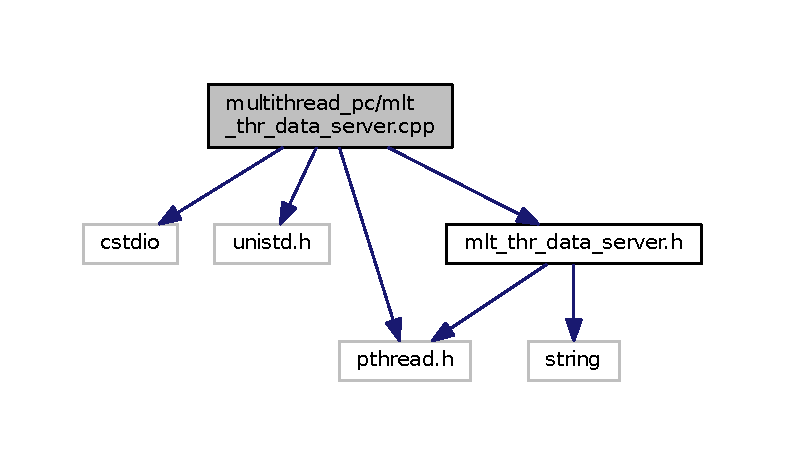
\includegraphics[width=350pt]{mlt__thr__data__server_8cpp__incl}
\end{center}
\end{figure}

\hypertarget{mlt__thr__data__server_8h}{}\section{multithread\+\_\+pc/mlt\+\_\+thr\+\_\+data\+\_\+server.h File Reference}
\label{mlt__thr__data__server_8h}\index{multithread\+\_\+pc/mlt\+\_\+thr\+\_\+data\+\_\+server.\+h@{multithread\+\_\+pc/mlt\+\_\+thr\+\_\+data\+\_\+server.\+h}}
{\ttfamily \#include $<$string$>$}\\*
{\ttfamily \#include $<$pthread.\+h$>$}\\*
Include dependency graph for mlt\+\_\+thr\+\_\+data\+\_\+server.\+h\+:
\nopagebreak
\begin{figure}[H]
\begin{center}
\leavevmode
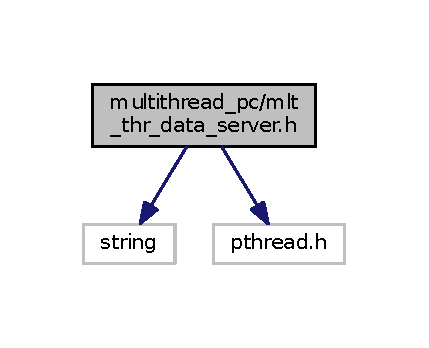
\includegraphics[width=206pt]{mlt__thr__data__server_8h__incl}
\end{center}
\end{figure}
This graph shows which files directly or indirectly include this file\+:
\nopagebreak
\begin{figure}[H]
\begin{center}
\leavevmode
\includegraphics[width=350pt]{mlt__thr__data__server_8h__dep__incl}
\end{center}
\end{figure}
\subsection*{Classes}
\begin{DoxyCompactItemize}
\item 
class \hyperlink{classMultiThreadDataServer}{Multi\+Thread\+Data\+Server}
\end{DoxyCompactItemize}

\hypertarget{prod__cons__simulator_8cpp}{}\section{multithread\+\_\+pc/prod\+\_\+cons\+\_\+simulator.cpp File Reference}
\label{prod__cons__simulator_8cpp}\index{multithread\+\_\+pc/prod\+\_\+cons\+\_\+simulator.\+cpp@{multithread\+\_\+pc/prod\+\_\+cons\+\_\+simulator.\+cpp}}
{\ttfamily \#include \char`\"{}prod\+\_\+cons\+\_\+simulator.\+h\char`\"{}}\\*
{\ttfamily \#include $<$iostream$>$}\\*
{\ttfamily \#include $<$random$>$}\\*
{\ttfamily \#include $<$ctime$>$}\\*
{\ttfamily \#include $<$cstdlib$>$}\\*
{\ttfamily \#include $<$unistd.\+h$>$}\\*
Include dependency graph for prod\+\_\+cons\+\_\+simulator.\+cpp\+:
\nopagebreak
\begin{figure}[H]
\begin{center}
\leavevmode
\includegraphics[width=350pt]{prod__cons__simulator_8cpp__incl}
\end{center}
\end{figure}
\subsection*{Functions}
\begin{DoxyCompactItemize}
\item 
void $\ast$ \hyperlink{prod__cons__simulator_8cpp_a555cff142ff5f082bf60983ed53e722b}{producer\+\_\+thread} (void $\ast$arg)
\item 
void $\ast$ \hyperlink{prod__cons__simulator_8cpp_a0d99d3bcb8787180b4227572fcf9240f}{consumer\+\_\+thread} (void $\ast$arg)
\end{DoxyCompactItemize}


\subsection{Function Documentation}
\index{prod\+\_\+cons\+\_\+simulator.\+cpp@{prod\+\_\+cons\+\_\+simulator.\+cpp}!consumer\+\_\+thread@{consumer\+\_\+thread}}
\index{consumer\+\_\+thread@{consumer\+\_\+thread}!prod\+\_\+cons\+\_\+simulator.\+cpp@{prod\+\_\+cons\+\_\+simulator.\+cpp}}
\subsubsection[{\texorpdfstring{consumer\+\_\+thread(void $\ast$arg)}{consumer_thread(void *arg)}}]{\setlength{\rightskip}{0pt plus 5cm}void$\ast$ consumer\+\_\+thread (
\begin{DoxyParamCaption}
\item[{void $\ast$}]{arg}
\end{DoxyParamCaption}
)}\hypertarget{prod__cons__simulator_8cpp_a0d99d3bcb8787180b4227572fcf9240f}{}\label{prod__cons__simulator_8cpp_a0d99d3bcb8787180b4227572fcf9240f}
\index{prod\+\_\+cons\+\_\+simulator.\+cpp@{prod\+\_\+cons\+\_\+simulator.\+cpp}!producer\+\_\+thread@{producer\+\_\+thread}}
\index{producer\+\_\+thread@{producer\+\_\+thread}!prod\+\_\+cons\+\_\+simulator.\+cpp@{prod\+\_\+cons\+\_\+simulator.\+cpp}}
\subsubsection[{\texorpdfstring{producer\+\_\+thread(void $\ast$arg)}{producer_thread(void *arg)}}]{\setlength{\rightskip}{0pt plus 5cm}void$\ast$ producer\+\_\+thread (
\begin{DoxyParamCaption}
\item[{void $\ast$}]{arg}
\end{DoxyParamCaption}
)}\hypertarget{prod__cons__simulator_8cpp_a555cff142ff5f082bf60983ed53e722b}{}\label{prod__cons__simulator_8cpp_a555cff142ff5f082bf60983ed53e722b}

\hypertarget{prod__cons__simulator_8h}{}\section{multithread\+\_\+pc/prod\+\_\+cons\+\_\+simulator.h File Reference}
\label{prod__cons__simulator_8h}\index{multithread\+\_\+pc/prod\+\_\+cons\+\_\+simulator.\+h@{multithread\+\_\+pc/prod\+\_\+cons\+\_\+simulator.\+h}}
{\ttfamily \#include \char`\"{}mlt\+\_\+thr\+\_\+data\+\_\+server.\+h\char`\"{}}\\*
{\ttfamily \#include $<$cstddef$>$}\\*
{\ttfamily \#include $<$string$>$}\\*
{\ttfamily \#include $<$memory$>$}\\*
{\ttfamily \#include $<$pthread.\+h$>$}\\*
Include dependency graph for prod\+\_\+cons\+\_\+simulator.\+h\+:
\nopagebreak
\begin{figure}[H]
\begin{center}
\leavevmode
\includegraphics[width=350pt]{prod__cons__simulator_8h__incl}
\end{center}
\end{figure}
This graph shows which files directly or indirectly include this file\+:
\nopagebreak
\begin{figure}[H]
\begin{center}
\leavevmode
\includegraphics[width=348pt]{prod__cons__simulator_8h__dep__incl}
\end{center}
\end{figure}
\subsection*{Classes}
\begin{DoxyCompactItemize}
\item 
class \hyperlink{classProdConsSimulator}{Prod\+Cons\+Simulator}
\end{DoxyCompactItemize}

\hypertarget{Readme_8md}{}\section{project/\+Readme.md File Reference}
\label{Readme_8md}\index{project/\+Readme.\+md@{project/\+Readme.\+md}}

%--- End generated contents ---

% Index
\backmatter
\newpage
\phantomsection
\clearemptydoublepage
\addcontentsline{toc}{chapter}{Index}
\printindex

\end{document}
